%%%%%%%%%%%%%%%%%%%%%%%%%%%%%%%%%%%%%%%%%%%%%%%%%%%%%%%%%%%%%%%%%%%%%%
% Template for a UBC-compliant dissertation
% At the minimum, you will need to change the information found
% after the "Document meta-data"
%
%!TEX TS-program = pdflatex
%!TEX encoding = UTF-8 Unicode

%% The ubcdiss class provides several options:
%%   gpscopy (aka fogscopy)
%%       set parameters to exactly how GPS specifies
%%         * single-sided
%%         * page-numbering starts from title page
%%         * the lists of figures and tables have each entry prefixed
%%           with 'Figure' or 'Table'
%%       This can be tested by `\ifgpscopy ... \else ... \fi'
%%   10pt, 11pt, 12pt
%%       set default font size
%%   oneside, twoside
%%       whether to format for single-sided or double-sided printing
%%   balanced
%%       when double-sided, ensure page content is centred
%%       rather than slightly offset (the default)
%%   singlespacing, onehalfspacing, doublespacing
%%       set default inter-line text spacing; the ubcdiss class
%%       provides \textspacing to revert to this configured spacing
%%   draft
%%       disable more intensive processing, such as including
%%       graphics, etc.
%%

% For submission to GPS
\documentclass[gpscopy,onehalfspacing,11pt]{ubcdiss}

% For your own copies (looks nicer)
% \documentclass[balanced,twoside,11pt]{ubcdiss}

%%%%%%%%%%%%%%%%%%%%%%%%%%%%%%%%%%%%%%%%%%%%%%%%%%%%%%%%%%%%%%%%%%%%%%
%%%%%%%%%%%%%%%%%%%%%%%%%%%%%%%%%%%%%%%%%%%%%%%%%%%%%%%%%%%%%%%%%%%%%%
%%
%% FONTS:
%% 
%% The defaults below configures Times Roman for the serif font,
%% Helvetica for the sans serif font, and Courier for the
%% typewriter-style font.  Configuring fonts can be time
%% consuming; we recommend skipping to END FONTS!
%% 
%% If you're feeling brave, have lots of time, and wish to use one
%% your platform's native fonts, see the commented out bits below for
%% XeTeX/XeLaTeX.  This is not for the faint at heart. 
%% (And shouldn't you be writing? :-)
%%

%% NFSS font specification (New Font Selection Scheme)
\usepackage{times,mathptmx,courier}
\usepackage[scaled=.92]{helvet}
\usepackage{todonotes}
\usepackage{mathtools}
%% Math or theory people may want to include the handy AMS macros
\usepackage{amssymb}
\usepackage{amsmath}
\usepackage{amsfonts}

%% The pifont package provides access to the elements in the dingbat font.   
%% Use \ding{##} for a particular dingbat (see p7 of psnfss2e.pdf)
%%   Useful:
%%     51,52 different forms of a checkmark
%%     54,55,56 different forms of a cross (saltyre)
%%     172-181 are 1-10 in open circle (serif)
%%     182-191 are 1-10 black circle (serif)
%%     192-201 are 1-10 in open circle (sans serif)
%%     202-211 are 1-10 in black circle (sans serif)
%% \begin{dinglist}{##}\item... or dingautolist (which auto-increments)
%% to create a bullet list with the provided character.
\usepackage{pifont}

%%%%%%%%%%%%%%%%%%%%%%%%%%%%%%%%%%%%%%%%%%%%%%%%%%%%%%%%%%%%%%%%%%%%%%
%% Configure fonts for XeTeX / XeLaTeX using the fontspec package.
%% Be sure to check out the fontspec documentation.
%\usepackage{fontspec,xltxtra,xunicode}	% required
%\defaultfontfeatures{Mapping=tex-text}	% recommended
%% Minion Pro and Myriad Pro are shipped with some versions of
%% Adobe Reader.  Adobe representatives have commented that these
%% fonts can be used outside of Adobe Reader.
%\setromanfont[Numbers=OldStyle]{Minion Pro}
%\setsansfont[Numbers=OldStyle,Scale=MatchLowercase]{Myriad Pro}
%\setmonofont[Scale=MatchLowercase]{Andale Mono}

%% Other alternatives:
%\setromanfont[Mapping=tex-text]{Adobe Caslon}
%\setsansfont[Scale=MatchLowercase]{Gill Sans}
%\setsansfont[Scale=MatchLowercase,Mapping=tex-text]{Futura}
%\setmonofont[Scale=MatchLowercase]{Andale Mono}
%\newfontfamily{\SYM}[Scale=0.9]{Zapf Dingbats}
%% END FONTS
%%%%%%%%%%%%%%%%%%%%%%%%%%%%%%%%%%%%%%%%%%%%%%%%%%%%%%%%%%%%%%%%%%%%%%
%%%%%%%%%%%%%%%%%%%%%%%%%%%%%%%%%%%%%%%%%%%%%%%%%%%%%%%%%%%%%%%%%%%%%%



%%%%%%%%%%%%%%%%%%%%%%%%%%%%%%%%%%%%%%%%%%%%%%%%%%%%%%%%%%%%%%%%%%%%%%
%%%%%%%%%%%%%%%%%%%%%%%%%%%%%%%%%%%%%%%%%%%%%%%%%%%%%%%%%%%%%%%%%%%%%%
%%
%% Recommended packages
%%
\usepackage{checkend}	% better error messages on left-open environments
\usepackage{graphicx}	% for incorporating external images

%% booktabs: provides some special commands for typesetting tables as used
%% in excellent journals.  Ignore the examples in the Lamport book!
\usepackage{booktabs}

%% listings: useful support for including source code listings, with
%% optional special keyword formatting.  The \lstset{} causes
%% the text to be typeset in a smaller sans serif font, with
%% proportional spacing.
\usepackage{listings}
\lstset{basicstyle=\sffamily\scriptsize,showstringspaces=false,fontadjust}

%% The acronym package provides support for defining acronyms, providing
%% their expansion when first used, and building glossaries.  See the
%% example in glossary.tex and the example usage throughout the example
%% document.
%% NOTE: to use \MakeTextLowercase in the \acsfont command below,
%%   we *must* use the `nohyperlinks' option -- it causes errors with
%%   hyperref otherwise.  See Section 5.2 in the ``LaTeX 2e for Class
%%   and Package Writers Guide'' (clsguide.pdf) for details.
\usepackage[printonlyused]{acronym}
%% The ubcdiss.cls loads the `textcase' package which provides commands
%% for upper-casing and lower-casing text.  The following causes
%% the acronym package to typeset acronyms in small-caps
%% as recommended by Bringhurst.
%\renewcommand{\acsfont}[1]{{\scshape \MakeTextLowercase{#1}}}

%% Commented out at stefan's behest for tooltip abbreviations
%\newcommand{\abbr}[1]{\pdftooltip{\ac*{#1}{\acl{#1}}\protect{\acused{#1}}}}
%\newcommand{\abbrIC}[1]{\pdftooltip{\ac*{#1}}{\acl{#1}}}

%% color: add support for expressing colour models.  Grey can be used
%% to great effect to emphasize other parts of a graphic or text.
%% For an excellent set of examples, see Tufte's "Visual Display of
%% Quantitative Information" or "Envisioning Information".
\usepackage{color}
\definecolor{greytext}{gray}{0.5}

%% comment: provides a new {comment} environment: all text inside the
%% environment is ignored.
%%   \begin{comment} ignored text ... \end{comment}
\usepackage{comment}

%% The natbib package provides more sophisticated citing commands
%% such as \citeauthor{} to provide the author names of a work,
%% \citet{} to produce an author-and-reference citation,
%% \citep{} to produce a parenthetical citation.
%% We use \citeeg{} to provide examples
\usepackage[numbers,sort&compress]{natbib}
\newcommand{\citeeg}[1]{\citep[e.g.,][]{#1}}

%% The titlesec package provides commands to vary how chapter and
%% section titles are typeset.  The following uses more compact
%% spacings above and below the title.  The titleformat that follow
%% ensure chapter/section titles are set in singlespace.
\usepackage[compact]{titlesec}
\titleformat*{\section}{\singlespacing\raggedright\bfseries\Large}
\titleformat*{\subsection}{\singlespacing\raggedright\bfseries\large}
\titleformat*{\subsubsection}{\singlespacing\raggedright\bfseries}
\titleformat*{\paragraph}{\singlespacing\raggedright\itshape}

%% The caption package provides support for varying how table and
%% figure captions are typeset.
\usepackage[format=hang,indention=-1cm,labelfont={bf},margin=1em]{caption}

%% url: for typesetting URLs and smart(er) hyphenation.
%% \url{http://...} 
\usepackage{url}
\urlstyle{sf}	% typeset urls in sans-serif


%%%%%%%%%%%%%%%%%%%%%%%%%%%%%%%%%%%%%%%%%%%%%%%%%%%%%%%%%%%%%%%%%%%%%%
%%%%%%%%%%%%%%%%%%%%%%%%%%%%%%%%%%%%%%%%%%%%%%%%%%%%%%%%%%%%%%%%%%%%%%
%%
%% Possibly useful packages: you may need to explicitly install
%% these from CTAN if they aren't part of your distribution;
%% teTeX seems to ship with a smaller base than MikTeX and MacTeX.
%%
%\usepackage{pdfpages}	% insert pages from other PDF files
%\usepackage{longtable}	% provide tables spanning multiple pages
%\usepackage{chngpage}	% support changing the page widths on demand
%\usepackage{tabularx}	% an enhanced tabular environment

%% enumitem: support pausing and resuming enumerate environments.
%\usepackage{enumitem}

%% rotating: provides two environments, sidewaystable and sidewaysfigure,
%% for typesetting tables and figures in landscape mode.  
%\usepackage{rotating}

%% subfig: provides for including subfigures within a figure,
%% and includes being able to separately reference the subfigures.
%\usepackage{subfig}

%% ragged2e: provides several new new commands \Centering, \RaggedLeft,
%% \RaggedRight and \justifying and new environments Center, FlushLeft,
%% FlushRight and justify, which set ragged text and are easily
%% configurable to allow hyphenation.
%\usepackage{ragged2e}

%% The ulem package provides a \sout{} for striking out text and
%% \xout for crossing out text.  The normalem and normalbf are
%% necessary as the package messes with the emphasis and bold fonts
%% otherwise.
%\usepackage[normalem,normalbf]{ulem}    % for \sout

%%%%%%%%%%%%%%%%%%%%%%%%%%%%%%%%%%%%%%%%%%%%%%%%%%%%%%%%%%%%%%%%%%%%%%
%% HYPERREF:
%% The hyperref package provides for embedding hyperlinks into your
%% document.  By default the table of contents, references, citations,
%% and footnotes are hyperlinked.
%%
%% Hyperref provides a very handy command for doing cross-references:
%% \autoref{}.  This is similar to \ref{} and \pageref{} except that
%% it automagically puts in the *type* of reference.  For example,
%% referencing a figure's label will put the text `Figure 3.4'.
%% And the text will be hyperlinked to the appropriate place in the
%% document.
%%
%% Generally hyperref should appear after most other packages

%% The following puts hyperlinks in very faint grey boxes.
%% The `pagebackref' causes the references in the bibliography to have
%% back-references to the citing page; `backref' puts the citing section
%% number.  See further below for other examples of using hyperref.
%% 2009/12/09: now use `linktocpage' (Jacek Kisynski): GPS now prefers
%%   that the ToC, LoF, LoT place the hyperlink on the page number,
%%   rather than the entry text.
\usepackage[bookmarks,bookmarksnumbered,%
    allbordercolors={0.8 0.8 0.8},%
    pagebackref,linktocpage%
    ]{hyperref}
%% The following change how the the back-references text is typeset in a
%% bibliography when `backref' or `pagebackref' are used
%%
%% Change \nocitations if you'd like some text shown where there
%% are no citations found (e.g., pulled in with \nocite{xxx})
\newcommand{\nocitations}{\relax}
%%\newcommand{\nocitations}{No citations}
%%
%\renewcommand*{\backref}[1]{}% necessary for backref < 1.33
\renewcommand*{\backrefsep}{,~}%
\renewcommand*{\backreftwosep}{,~}% ', and~'
\renewcommand*{\backreflastsep}{,~}% ' and~'
\renewcommand*{\backrefalt}[4]{%
\textcolor{greytext}{\ifcase #1%
\nocitations%
\or
\(\rightarrow\) page #2%
\else
\(\rightarrow\) pages #2%
\fi}}


%% The following uses most defaults, which causes hyperlinks to be
%% surrounded by colourful boxes; the colours are only visible in
%% PDFs and don't show up when printed:
%\usepackage[bookmarks,bookmarksnumbered]{hyperref}

%% The following disables the colourful boxes around hyperlinks.
%\usepackage[bookmarks,bookmarksnumbered,pdfborder={0 0 0}]{hyperref}

%% The following disables all hyperlinking, but still enabled use of
%% \autoref{}
%\usepackage[draft]{hyperref}

%% The following commands causes chapter and section references to
%% uppercase the part name.
\renewcommand{\chapterautorefname}{Chapter}
\renewcommand{\sectionautorefname}{Section}
\renewcommand{\subsectionautorefname}{Section}
\renewcommand{\subsubsectionautorefname}{Section}

%% If you have long page numbers (e.g., roman numbers in the 
%% preliminary pages for page 28 = xxviii), you might need to
%% uncomment the following and tweak the \@pnumwidth length
%% (default: 1.55em).  See the tocloft documentation at
%% http://www.ctan.org/tex-archive/macros/latex/contrib/tocloft/
% \makeatletter
% \renewcommand{\@pnumwidth}{3em}
% \makeatother

%%%%%%%%%%%%%%%%%%%%%%%%%%%%%%%%%%%%%%%%%%%%%%%%%%%%%%%%%%%%%%%%%%%%%%
%%%%%%%%%%%%%%%%%%%%%%%%%%%%%%%%%%%%%%%%%%%%%%%%%%%%%%%%%%%%%%%%%%%%%%
%%
%% Some special settings that controls how text is typeset
%%
% \raggedbottom		% pages don't have to line up nicely on the last line
% \sloppy		% be a bit more relaxed in inter-word spacing
% \clubpenalty=10000	% try harder to avoid orphans
% \widowpenalty=10000	% try harder to avoid widows
% \tolerance=1000

%% And include some of our own useful macros
% This file provides examples of some useful macros for typesetting
% dissertations.  None of the macros defined here are necessary beyond
% for the template documentation, so feel free to change, remove, and add
% your own definitions.
%
% We recommend that you define macros to separate the semantics
% of the things you write from how they are presented.  For example,
% you'll see definitions below for a macro \file{}: by using
% \file{} consistently in the text, we can change how filenames
% are typeset simply by changing the definition of \file{} in
% this file.
% 
%% The following is a directive for TeXShop to indicate the main file
%%!TEX root = diss.tex

\newcommand{\NA}{\textsc{n/a}}	% for "not applicable"
\newcommand{\eg}{e.g.,\ }	% proper form of examples (\eg a, b, c)
\newcommand{\ie}{i.e.,\ }	% proper form for that is (\ie a, b, c)
\newcommand{\etal}{\emph{et al}}

% Some useful macros for typesetting terms.
\newcommand{\file}[1]{\texttt{#1}}
\newcommand{\class}[1]{\texttt{#1}}
\newcommand{\latexpackage}[1]{\href{http://www.ctan.org/macros/latex/contrib/#1}{\texttt{#1}}}
\newcommand{\latexmiscpackage}[1]{\href{http://www.ctan.org/macros/latex/contrib/misc/#1.sty}{\texttt{#1}}}
\newcommand{\env}[1]{\texttt{#1}}
\newcommand{\BibTeX}{Bib\TeX}

% Define a command \doi{} to typeset a digital object identifier (DOI).
% Note: if the following definition raise an error, then you likely
% have an ancient version of url.sty.  Either find a more recent version
% (3.1 or later work fine) and simply copy it into this directory,  or
% comment out the following two lines and uncomment the third.
\DeclareUrlCommand\DOI{}
\newcommand{\doi}[1]{\href{http://dx.doi.org/#1}{\DOI{doi:#1}}}
%\newcommand{\doi}[1]{\href{http://dx.doi.org/#1}{doi:#1}}

% Useful macro to reference an online document with a hyperlink
% as well with the URL explicitly listed in a footnote
% #1: the URL
% #2: the anchoring text
\newcommand{\webref}[2]{\href{#1}{#2}\footnote{\url{#1}}}

% epigraph is a nice environment for typesetting quotations
\makeatletter
\newenvironment{epigraph}{%
	\begin{flushright}
	\begin{minipage}{\columnwidth-0.75in}
	\begin{flushright}
	\@ifundefined{singlespacing}{}{\singlespacing}%
    }{
	\end{flushright}
	\end{minipage}
	\end{flushright}}
\makeatother

% \FIXME{} is a useful macro for noting things needing to be changed.
% The following definition will also output a warning to the console
\newcommand{\FIXME}[1]{\typeout{**FIXME** #1}\textbf{[FIXME: #1]}}

% END


%%%%%%%%%%%%%%%%%%%%%%%%%%%%%%%%%%%%%%%%%%%%%%%%%%%%%%%%%%%%%%%%%%%%%%
%%%%%%%%%%%%%%%%%%%%%%%%%%%%%%%%%%%%%%%%%%%%%%%%%%%%%%%%%%%%%%%%%%%%%%
%%
%% Document meta-data: be sure to also change the \hypersetup information
%%

\title{Exploring the tumour microenvironment with non-invasive Magnetic Resonance Imaging techniques}
%\subtitle{If you want a subtitle}

\author{Firas Moosvi}
\previousdegree{Master of Science, University of Toronto, 2012}
\previousdegree{Bachelor of Science, University of British Columbia, 2009}

% What is this dissertation for?
\degreetitle{Doctor of Philosophy}

\institution{The University of British Columbia}
\campus{Vancouver}

\faculty{The Faculty of Science}
\department{Physics \& Astronomy}
\submissionmonth{May}
\submissionyear{2019}

%% hyperref package provides support for embedding meta-data in .PDF
%% files
\hypersetup{
  pdftitle={Exploring the tumour microenvironment with non-invasive Magnetic Resonance Imaging techniques (DRAFT: \today)},
  pdfauthor={Firas Moosvi},
  pdfkeywords={MRI, Cancer, tumours, HPG, contrast agents, oxygen enhanced MRI}
}

\usepackage{pdfcomment}
\newcommand{\abbr}[1]{\pdftooltip{\ac*{#1}}{\acl*{#1}}\acused{#1}}

%%%%%%%%%%%%%%%%%%%%%%%%%%%%%%%%%%%%%%%%%%%%%%%%%%%%%%%%%%%%%%%%%%%%%%
%%%%%%%%%%%%%%%%%%%%%%%%%%%%%%%%%%%%%%%%%%%%%%%%%%%%%%%%%%%%%%%%%%%%%%
%% 
%% The document content
%%

%% LaTeX's \includeonly commands causes any uses of \include{} to only
%% include files that are in the list.  This is helpful to produce
%% subsets of your thesis (e.g., for committee members who want to see
%% the dissertation chapter by chapter).  It also saves time by 
%% avoiding reprocessing the entire file.
%\includeonly{intro,conclusions}
%\includeonly{discussion}

\begin{document}

%%%%%%%%%%%%%%%%%%%%%%%%%%%%%%%%%%%%%%%%%%%%%%%%%%
%% From Thesis Components: Tradtional Thesis
%% <http://www.grad.ubc.ca/current-students/dissertation-thesis-preparation/order-components>

% Preliminary Pages (numbered in lower case Roman numerals)
%    1. Title page (mandatory)
\maketitle

%    2. Abstract (mandatory - maximum 350 words)
%%% The following is a directive for TeXShop to indicate the main file
%%!TEX root = diss.tex

\chapter{Abstract}

This thesis comprises development and application of several MRI techniques to improve our understanding of tumour growth, drug distribution, and drug effect using pre-clinical tumour models in mice. In the first part of the thesis, a novel high molecular weight contrast agent, HPG-GdF is introduced. This molecule is a hyperbranched polyglycerol labeled with an MRI contrast agent (Gd-DOTA) as well as a fluorescent tag. After injecting the agent into mice within an MRI scanner, contrast-agent kinetics were quantified using a two-parameter linear model and validated with quantitative immunohistochemistry via direct fluorescence imaging of HPG-GdF.

HPG-GdF was used to assess whether vascular function plays a role in how a chemotherapy (Herceptin) distributes within a tumour. Tumour vessel permeability and fractional plasma volume were quantified using the HPG-GdF and no relationship was found between vascular function and presence of drug. HPG-GdF was then applied to show that Avastin (an antiangiogenic agent) decreased vessel permeability in tumours. Using histological methods, a dramatic reduction in hypoxia (oxygen deficiency in tissues) was observed in treated tumours. Unfortunately, existing MRI methods to evaluate oxygenation were time-intensive and lacked sensitivity. In the second part of this thesis, we introduce, develop, validate, and apply a new method to assess tumour oxygenation using MRI. 

Oxygen (O$_2$) is a paramagnetic molecule that shortens the longitudinal relaxation time (T$_1$) of protons in MRI. This subtle effect has been widely reported in the literature but its applications in cancer have been limited. Our technique - dynamic oxygen-enhanced MRI (\acs{dOE-MRI}) - uses T$_1$W signal intensity images acquired during a cycling gas challenge (air or oxygen) and independent component analysis (ICA). Hypoxia staining with pimonidazole correlated strongly with \acs{dOE-MRI} values in a murine tumour model (SCCVII) and only weakly in a colorectal xenograft model (HCT-116). Finally, we provide compelling evidence that treatment with Avastin improves tumour oxygenation in subcutaneous tumours. With \acs{dOE-MRI}, the sensitivity and speed of existing techniques was greatly improved. Since our technique requires no injectable contrast agent, special sequences or hardware, we anticipate that this technique can be quickly translated into the clinic. 


% Consider placing version information if you circulate multiple drafts
\vfill
\begin{center}
\begin{sf}
\fbox{Git commit: d81f849}
\end{sf}
\end{center}

\cleardoublepage

%    3. Lay Summary (Effective May 2017, mandatory - maximum 150 words)
%%% The following is a directive for TeXShop to indicate the main file
%%!TEX root = diss.tex

%% https://www.grad.ubc.ca/current-students/dissertation-thesis-preparation/preliminary-pages
%% 
%% LAY SUMMARY Effective May 2017, all theses and dissertations must
%% include a lay summary.  The lay or public summary explains the key
%% goals and contributions of the research/scholarly work in terms that
%% can be understood by the general public. It must not exceed 150
%% words in length.

\chapter{Lay Summary}

In this thesis we have described the development and application of several magnetic resonance imaging (MRI) techniques to improve our understanding of tumour in mice.
In the first part of the thesis, a new analysis method was outlined to characterize tumour blood vessels with a novel bio-compatible contrast agent.
In the second part of this thesis, we introduced, developed, validated, and applied a new method to assess tumour oxygenation using MRI.
Our technique is a significant improvement over other available methods as it uses a machine learning technique to extract very small changes in MRI signal just by inhaling 100\% oxygen gas. 
We used this technique to show that treatment with a cancer drug that prunes malformed and abnormal blood vessels in tumour improves oxygenation levels.
Since our technique requires no injectable contrast agent, special sequences or hardware, we anticipate that this technique can be quickly translated into the clinic. 

\cleardoublepage

%    4. Preface
%%% The following is a directive for TeXShop to indicate the main file
%%!TEX root = diss.tex

\chapter{Preface}

At \ac{UBC}, a preface may be required.  Be sure to check the
\ac{GPS} guidelines as they may have specific content to be included.

\cleardoublepage

%    5. Table of contents (mandatory - list all items in the preliminary pages
%    starting with the abstract, followed by chapter headings and
%    subheadings, bibliographies and appendices)
\tableofcontents
\cleardoublepage	% required by tocloft package

%    6. List of tables (mandatory if thesis has tables)
\listoftables
\cleardoublepage	% required by tocloft package

%    7. List of figures (mandatory if thesis has figures)
\listoffigures
\cleardoublepage	% required by tocloft package

%    8. List of illustrations (mandatory if thesis has illustrations)
%    9. Lists of symbols, abbreviations or other (optional)

%   10. Glossary (optional)
%% The following is a directive for TeXShop to indicate the main file
%%!TEX root = diss.tex

\chapter{Glossary}

% use \acrodef to define an acronym, but no listing
\acrodef{UI}{user interface}
\acrodef{UBC}{University of British Columbia}

\acrodef{DCE-US}{dynamic contrast enhanced ultrasound}
\acrodef{ICA}{Independent Component Analysis}


% The acronym environment will typeset only those acronyms that were
% *actually used* in the course of the document
\begin{acronym}

\acro{ICA}[ICA]{Independent Component Analysis; a blind source separation technique that splits a multi-source signal into its constituents}

\acro{dOE-MRI}[dOE-MRI]{dynamic Oxygen Enhanced MRI; a technique that relies on the T$_1$-shortening property of oxygen and independent component analysis to identify regions that respond to an oxygen stimulus.}

\acro{DCE-US}[DCE-US]{dynamic contrast enhanced ultrasound; an imaging technique that uses echogenic microbubbles to enhance contrast \emph{in vivo}.}

\acro{CD31}[CD31]{cluster of differentiation 31 (CD31), also known as platelet endothelial cell adhesion molecule (PECAM) is a protein that is used in immunohistochemistry primarily to demonstrate the presence of endothelial cells.}

\acro{Hoechst 33342}[bisbenzimide]{Hoechst 33342 (also known as bisbenzimide) is an organic compound used as a fluorescent stain for DNA}

\acro{EPR}[EPR]{EPR, or enhanced permeability and retention is a phenomenon that results in macromolecules are retained in the tumour and extravasation into the tumour interstitium continues due to poor lymphatic clearance and other factors.}

\acro{CA}[CA]{Contrast agent}

\acro{MCA}[MCA]{Macromolecular contrast agents.}

\acro{aPS}[aPS]{Apparent permeability surface area product; a parameter derived from DCE-MRI using HPG}

\acro{fPV}[fPV]{Fractional plasma volume}

\acro{HPG-GdF}[HPG-GdF]{Hyperbranched polyglycerol (HPG) chelated to Gd-DTPA with a fluorophore (F) attached; 500 kDa) }

\acro{MW}[MW]{Molcular weight}

\acro{MAb}[MAb]{Monoclonal antibody}
\acroplural{MAbs}[MAbs]{Monoclonal antibodies}
\acro{}[]{}
\acro{}[]{}
\acro{}[]{}
\acro{}[]{}
\acro{}[]{}
\acro{}[]{}



\end{acronym}

% You can also use \newacro{}{} to only define acronyms
% but without explictly creating a glossary
% 
% \newacro{ANOVA}[ANOVA]{Analysis of Variance\acroextra{, a set of
%   statistical techniques to identify sources of variability between groups.}}
% \newacro{API}[API]{application programming interface}
% \newacro{GOMS}[GOMS]{Goals, Operators, Methods, and Selection\acroextra{,
%   a framework for usability analysis.}}
% \newacro{TLX}[TLX]{Task Load Index\acroextra{, an instrument for gauging
%   the subjective mental workload experienced by a human in performing
%   a task.}}
% \newacro{UI}[UI]{user interface}
% \newacro{UML}[UML]{Unified Modelling Language}
% \newacro{W3C}[W3C]{World Wide Web Consortium}
% \newacro{XML}[XML]{Extensible Markup Language}
	% always input, since other macros may rely on it
%%% The following is a directive for TeXShop to indicate the main file
%%!TEX root = diss.tex

\chapter{Acro-Glossary}

 \ac{cd} \ac{mc}\par\vspace{1cm}
 \ac{cd} \ac{mc}

 \aca{cd} \aca{mc}

 \acs{cd} \acs{mc}	% always input, since other macros may rely on it


\textspacing		% begin one-half or double spacing

%   11. Acknowledgements (optional)
%% The following is a directive for TeXShop to indicate the main file
%%!TEX root = diss.tex

\chapter{Acknowledgments}

This work would not be possible without the tireless commitment and mentoring by my supervisor, Dr. Stefan Reinsberg.
Dr. Baker was also instrumental in helping run, plan, and provide support for all of the work presented here. 
Members of my supervisory committee, Drs. Kozlowski, Laule, and Minchinton were excellent sources of advice, feedback, guidance, and general project direction. 
Particular thanks to Dr. Kozlowski for supporting and organizing weekly lab meetings giving me and other trainees to give and get honest feedback on preliminary work - I learned a tonne through these meetings.

Finally, a huge thanks goes to my family, and my wife who has supported and humoured me through my meanderings over the course of my PhD. 

%   12. Dedication (optional)

% Body of Thesis (not all sections may apply)
\mainmatter

\acresetall	% reset all acronyms used so far

%    1. Introduction
%% The following is a directive for TeXShop to indicate the main file
%%!TEX root =../diss.tex

\chapter{Introduction}
\label{ch:Introduction}

\section{Cancer}

Some facts about prevalence of cancer and poor outcomes, high toxicity to motivate this work.\todo[backgroundcolor=red!20!white]{to fix}

\todo[backgroundcolor=red!20!white]{this section needs a thorough re-write i think}
\subsection{Current therapies}
\todo[backgroundcolor=red!20!white]{Change title to less broad (from SAR)}
Numerous advancements in chemotherapies over the past decade have sparked an urgent clinical need for non-invasive methods to assess treatment efficacy.
There is a knowledge gap in the use and synergistic combinations of therapies, and many treatment regimens expose patients to higher toxicity than necessary.
Despite known extremes in patient response to treatment - even in cancers of the same type and grade - doses are generally prescribed by success rates of trials in patient populations exhibiting similar disease manifestations.
Each class of drugs has unique modes of action and still, there are no reliable and reproducible methods to assess synergistic benefits of combined therapy regimens~\cite{Zhang:2008ie}.
Traditionally, a prominent measure of treatment response has been to track tumour shrinkage following treatment~\cite{Tuma:2006hx}.
However, it has been shown that tumour shrinkage can take weeks and sometimes even months to manifest~\cite{Brindle:2008jt} and in some cases may not occur at all~\cite{Kitzen:2008un}.
For instance, anti-angiogenic agents typically arrest tumour growth by disrupting existing vasculature or inhibiting new vessel growth.
Despite positive effect, these agents may not necessarily lead to tumour shrinkage.
This mode of drug action is better characterized by assessing tumour vascular function rather than gross changes in physical size.
Development of quantitative and non-invasive methods to assess tumours following therapy continues to be a burgeoning field.
Furthermore, there is an urgent need in the drug development and testing community as drugs that fail in the late stages of clinical trials have led to an astronomical rise in the cost of developing drugs.
Lack of effective patient stratification techniques to identify potential responders from non-responders is a key reason that drugs fail.
For instance clinical trials targeting hypoxia - a key target for both chemotherapy to improve drug delivery and radiotherapy to increase radiosensitivity - have been conducted without patient selection or stratification based on pre-treatment tumour hypoxia status and therefore include patients with different hypoxic fractions~\cite{Overgaard:2011ji}.
This is at least partially due to an absence of validated methods that can accurately assess the hypoxia status of tumours \emph{in vivo}.
The benefits of developing early, non-invasive measures of treatment efficacy are clear for both patients and health care systems.
For patients, if a standard treatment regimen is prescribed and deemed ineffective early, the treatment can be altered and patients can directly benefit from personalized care.
Similarly, with improved patient stratification using non-invasive gross assessments of the tumour status, these patients can avoid receiving ineffective and expensive therapies.
However, the choice of appropriate biomarkers for many targets remains elusive. 

\subsection{Cancer Biomarkers and targets} There has been considerable interest in predictive biomarkers for early assessment.
Several candidates have appeared and disappeared but in 2000, a seminal paper catalogued a vast array of cancer cell genotypes into ``six essential alterations in cell physiology that collectively dictate malignant growth in tumours''~\cite{Hanahan:2000wo} (figure~\ref{cancerHallmarks}): 1) self-sufficiency in growth signals, 2) insensitivity to growth-inhibitory signals, 3) evasion of programmed cell death, 4) limitless replicative potential, 5) sustained angiogenesis and, 6) tissue invasion and metastasis~\cite{Hanahan:2000wo}.
In 2011, taking into account the progress made over a decade, the framework expanded to inculde four more hallmarks for the next generation~\cite{Hanahan:2011gu}.
Angiogenesis, the 5th hallmark is particularly suitable for consideration in non-invasive imaging techniques, particularly MRI. 

\begin{figure}[htbp]   
 \begin{center}  
 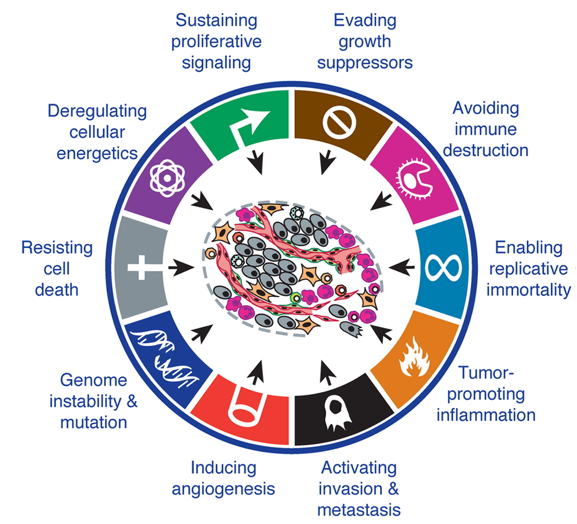
\includegraphics[width=4in]{intro/./intro-images/cancerHallmarks.png}
 \caption{Graphical illustration of the hallmarks of cancer; many of these targets are inaccessible to non-invasive imaging. Figure from the Hanahan group~\cite{Hanahan:2011gu}.}  
 \label{cancerHallmarks}  
 \end{center}
\end{figure}

Angiogenesis, or the formation of new blood vessels from pre-existing ones is a normal and vital process in the body tightly regulated by various cell signalling pathways and growth factors.
In tumours, angiogenesis is a critical step in the growth and spread of tumours as new blood vessels are recruited from the existing vascular network to promote rapidly accelerated and abnormal tumour growth~\cite{Folkman:1990ud}.
Normally, this process is regulated by several angiogenic and antiangiogenic factors such as $\alpha \beta$ integrin, vascular endothelial growth factor (VEGF) and fibroblast growth factor~\cite{Laking:2006ij}.
In tumours however, this process is completely deregulated (figure~\ref{tumourVasculature}) and excess production of growth factors from rapidly proliferating tumour cells leads to a drastic increase in vasculogenesis.
These newly formed vessels are unstable and must mature with the addition of pericytes, cells that surround the endothelium providing structural support.
Pericytes are often malformed and poorly distributed in solid tumours contributing to a dysfunctional vascular network.
Vessel growth patterns in tumours are generally accepted to be abnormal with a defective and leaky endothelium~\cite{McDonald:2002ut}.
Irregular diameters of tumour vessels, abnormal branching patterns and leaky vessel walls all contribute to an increase in vessel permeability.
It is estimated that a single hole larger than 0.5$\mu$m in diameter would alter the permeability of that vessel significantly enough to result in solute extravasation to be limited by blood flow~\cite{McDonald:2002ut}.
Disorganized and inefficient blood flow also limits the delivery of macromolecules, such as chemotherapeutic agents via the blood.
Poor perfusion in the tumour due to a disorganized vascular network impairs the delivery of systemic drugs to the whole tumour and ultimately, reduces efficacy. 

%\begin{wrapfigure}{L}{0.65\textwidth} 
\begin{figure}  
 \begin{center}  
 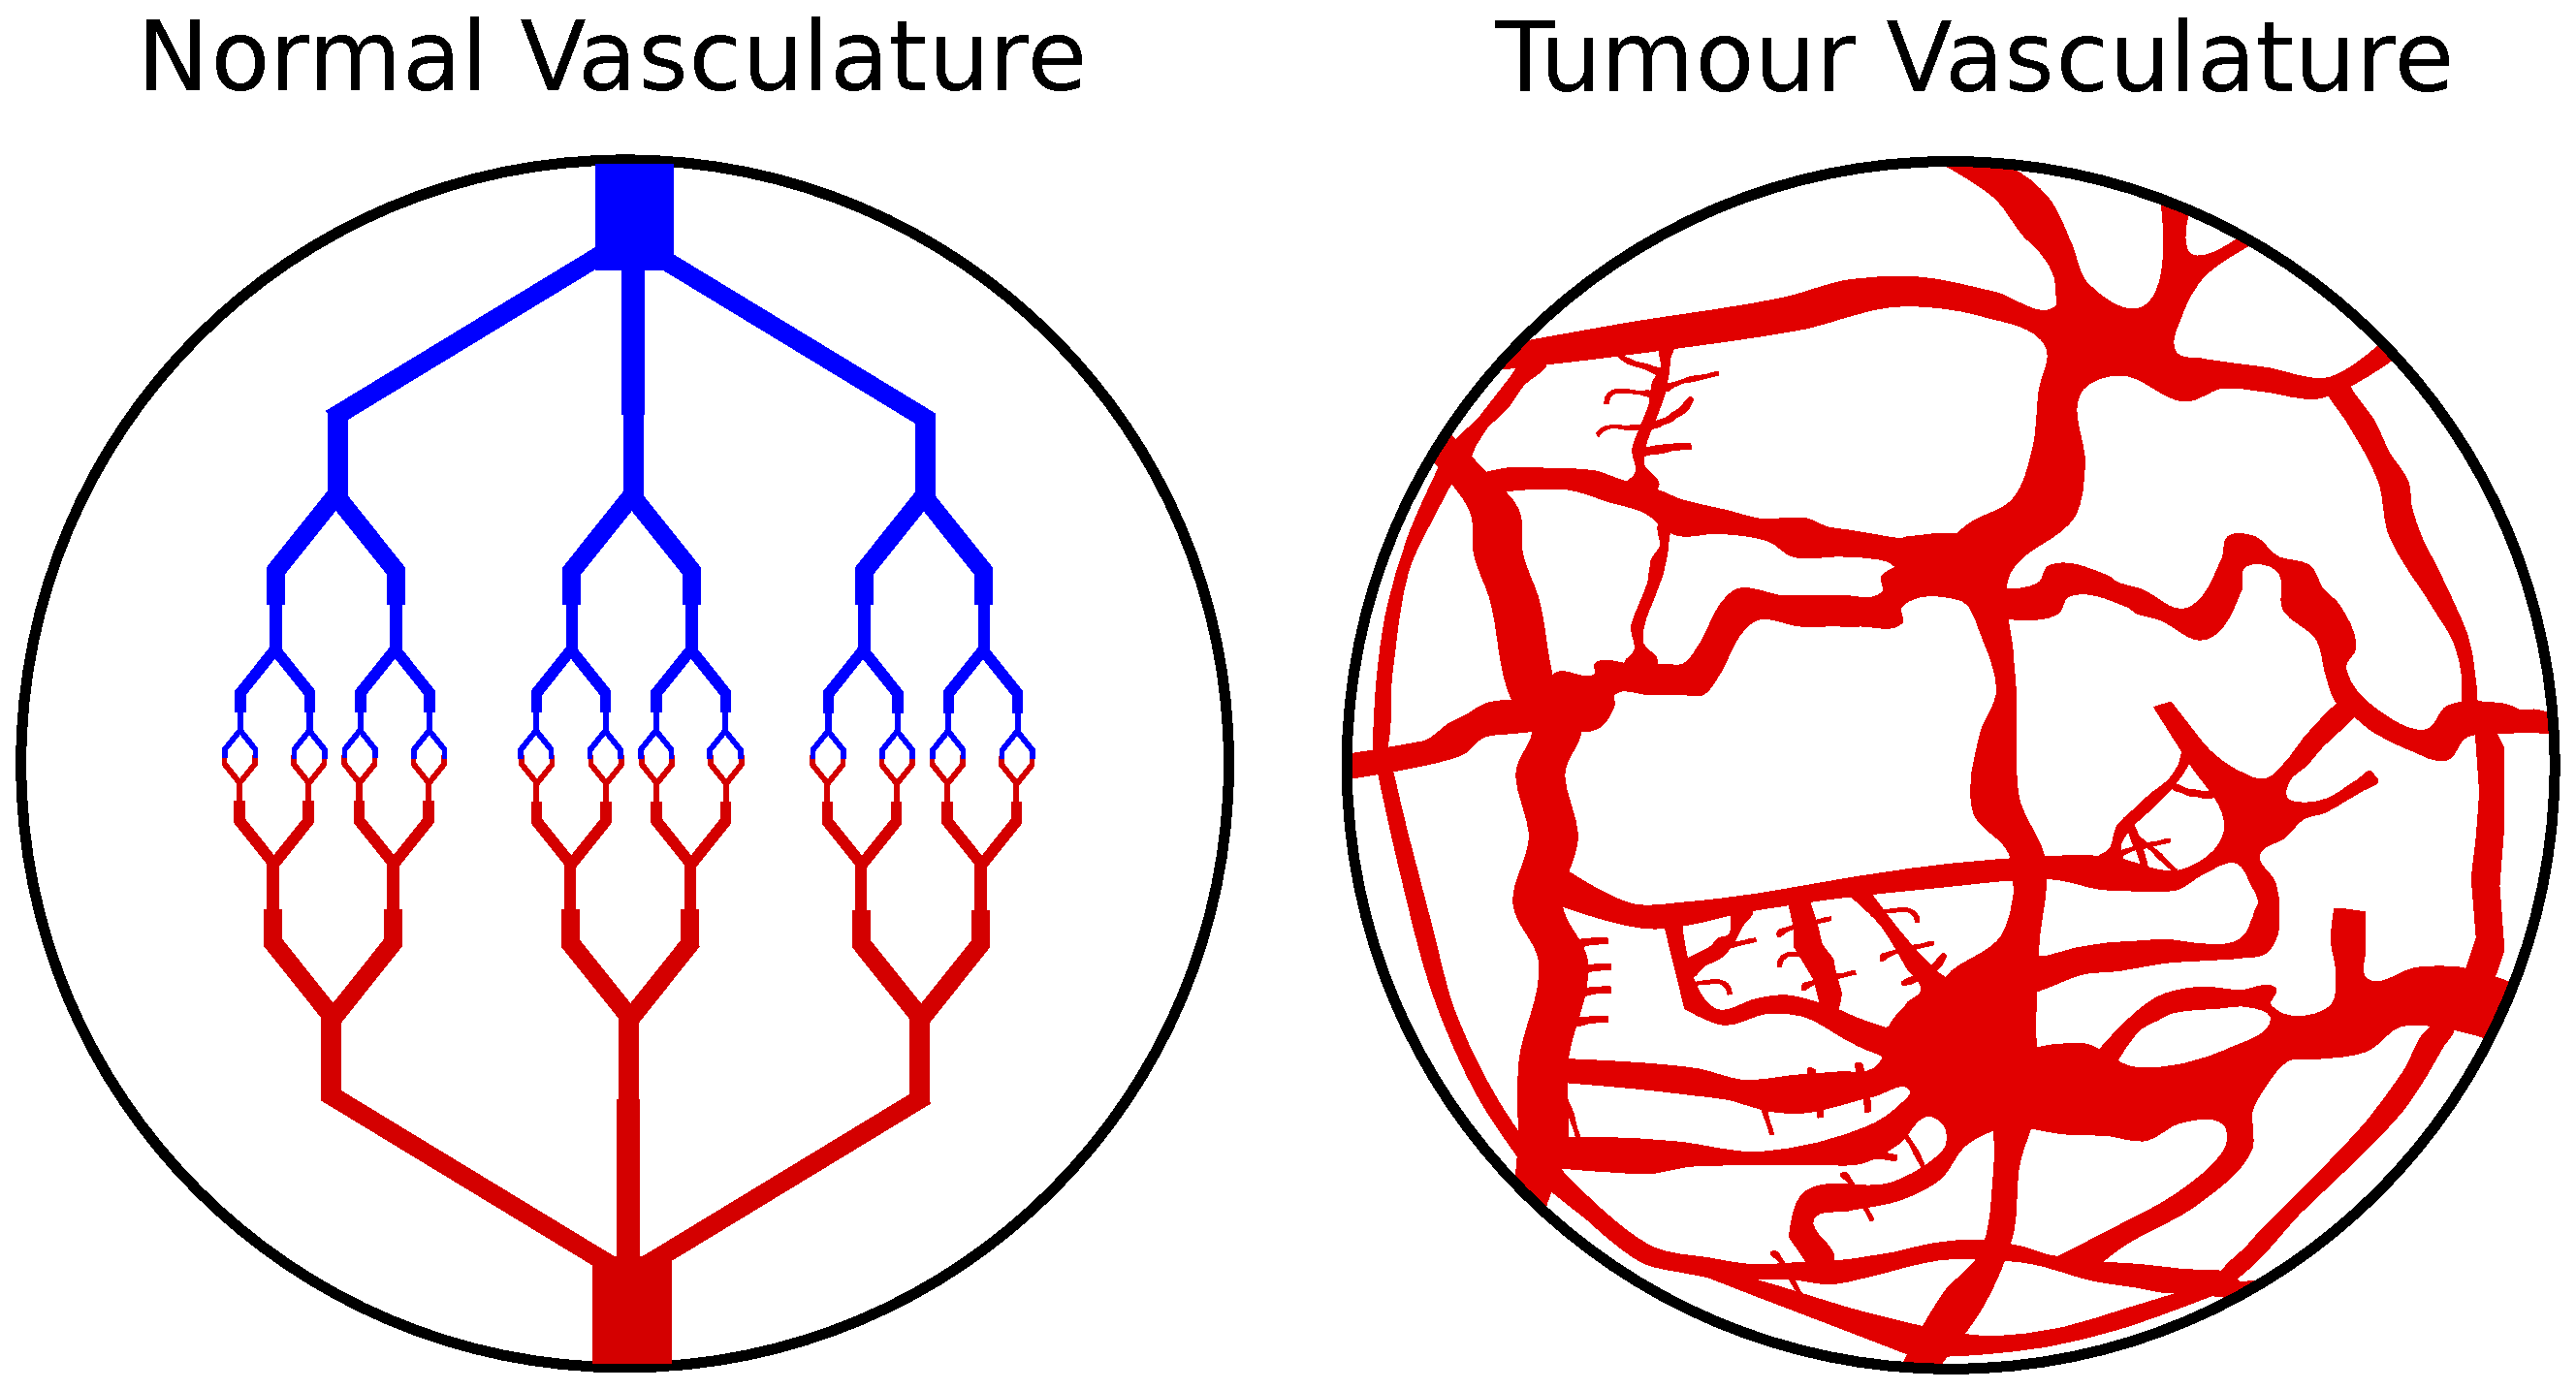
\includegraphics[width=4in]{intro/intro-images/tumourVasculature.pdf}
 \caption{Schematic of the normal tissue (left) and tumour (right) vasculature network. 
 Note the hierarchical structure of oxygenated blood (red) passing through the arteries, arterioles, and deoxygenated blood leaving via the venules, veins. 
 In tumours, this structure is severely compromised and often, no clear flow patterns can be distinguished with many vessels ending in dead ends or looping back onto feeding vessels.}
 \label{tumourVasculature}
 \end{center}
\end{figure}

Several strategies have been proposed to maximize cell kill, including the combination of different therapies (such as radiotherapy and chemotherapy) and agents that ``normalize'' the tumour vasculature and prime them for receiving chemotherapies~\cite{Jain:2005gk}.
Tumour angiogenesis is extremely important in tumour growth, progression and metastasis and is a promising target for novel therapies~\cite{Miles:2000wq}.
For instance, ``measuring'' tumour angiogenesis has the potential to serve as a highly predictive prognostic marker for disease outcome and treatment.
Histology remains the gold standard for angiogenesis detection (microvessel density) but has several critical limitations.
Histology requires biopsy samples and patient comfort aside, biopsies only sample a small fraction of the potentially affected organ.
The lack of functional information from biopsies as well as the practical challenges of obtaining longitudinal biopsy samples make non-invasive imaging a promising technique to complement and potentially reduce unneeded biopsies.

\subsection{Need for non-invasive imaging}
Non-invasive imaging methods are proving indispensable for studying angiogenesis \emph{in vivo} as they provide researchers with quantitative information about blood flow, vascular permeability, vessel density, vessel function and blood volume~\cite{McDonald:2003cm}.
Imaging modalities such as computed tomography (CT), magnetic resonance imaging (MRI), positron emission tomography (PET), single photon emission computed tomography (SPECT) and ultrasound (US), have all been proposed for studying angiogenesis~\cite{Laking:2006ij}.
Each modality is optimal for probing a particular aspect of biomarkers. To study angiogenesis and its effects on tumour growth and treatment response, the tumour environment needs to be probed using tools that assess both the interstitial tumour volume as well as the tumour vasculature.
Nuclear medicine techniques such as PET and SPECT employ radiotracers that can be measured at picomolar concentrations but at a significantly lower spatial resolution.
DCE-MRI and DCE-CT offer similar perfusion measurements (rate of leakage and leakage space) as both rely on the administration of a contrast agent that diffuses from the vasculature.
DCE-CT is advantageous as it has a direct linear relationship between the contrast agent concentration and the image intensity (attenuation numbers, given by Houndsfield Units)~\cite{Cuenod:2006jy}.
The disadvantage of CT however is that it requires ionizing radiation and iodinated contrast agents used in CT have been shown to have lower safety profiles compared to MR contrast agents~\cite{Hasebroock:2009hw}.
MRI can also be used to measure additional information such as diffusion, tissue oxygenation, spectroscopy, chemical exchange and magnetization transfer. 
In this thesis, several techniques will be explored in a bid to improve our understanding of the tumour microenvironment.

\section{Magnetic Resonance Imaging}

In biological specimens, water is by far the most abundant molecule in the body and the hydrogen atom in water is central to MR imaging.
Other MR-active atoms include $^{13}$C, $^{19}$F, $^{23}$Na and $^{31}$P, but these are rare and not used in this thesis.
We begin our description of the principles of magnetic resonance imaging, outside the scanner in a bucket of water.
The molecular mass of a water molecule (H$_2$O) is approximately 18 g/mol and its density is 1 g/mL so in this 1L bucket, there are approximately 3$\times10^{25}$ molecules of water.
Moving from macroscopic to microscopic, each molecule of water contains two hydrogen atoms and one oxygen atom.
Within the nucleus of a hydrogen atom, there is a single proton, resulting in a net positive charge on the atom.
An intrinsic property of fundamental particles such as the proton and neutron is that they posses spin angular momentum.
Incidentally, spin is the only quantum mechanics required to understand the vast majority of MR principles~\cite{Hanson:2008tp}.
Nuclei ``inherit'' this quantum mechanical property from its constituent subatomic particles - in particular, neutrons and protons.
The nucleus of a hydrogen atom has an odd number of protons (n=1) so there is a net spin angular momentum.
This results in the nucleus having an intrinsic magnetic moment arising from the net nuclear spin angular momentum and net charge from the proton.
Though there is no analogy to this from a classical physics perspective, one can imagine the net magnetic moment of a proton as a close cousin to the classical situation of the magnetic field generated by a loop of current in a wire.
To summarize, each proton in the hydrogen nucleus has spin angular momentum, is charged and thus has a net magnetic moment.

We will model the hydrogen atom with a net magnetic moment as a small bar magnet spinning on its own axis (with an arrow vector representing the direction and strength of the magnetic moment) and rely on classical physics to describe the principle of magnetic resonance imaging. 
If a spinning bar magnet is placed in an external magnetic field, the magnetic moment vector of the bar magnet will precess, or rotate about the new magnetic field with a frequency known as the Larmor frequency:

\begin{equation}
	\omega = \gamma \vec{\mathbf{B_0}}
\end{equation}

The proportionality factor $\gamma$ is the gyromagnetic ratio and is nuclei-dependent and for protons, $\gamma = 42 MhZ /T$.
For convenience it is useful to change our reference frame to a rotating reference frame so the the magnetic moment vector is stationary on a (rotating) cartesian axis.
\todo[backgroundcolor=red!20!white]{add caption to this figure}
\begin{figure}
	\centering
	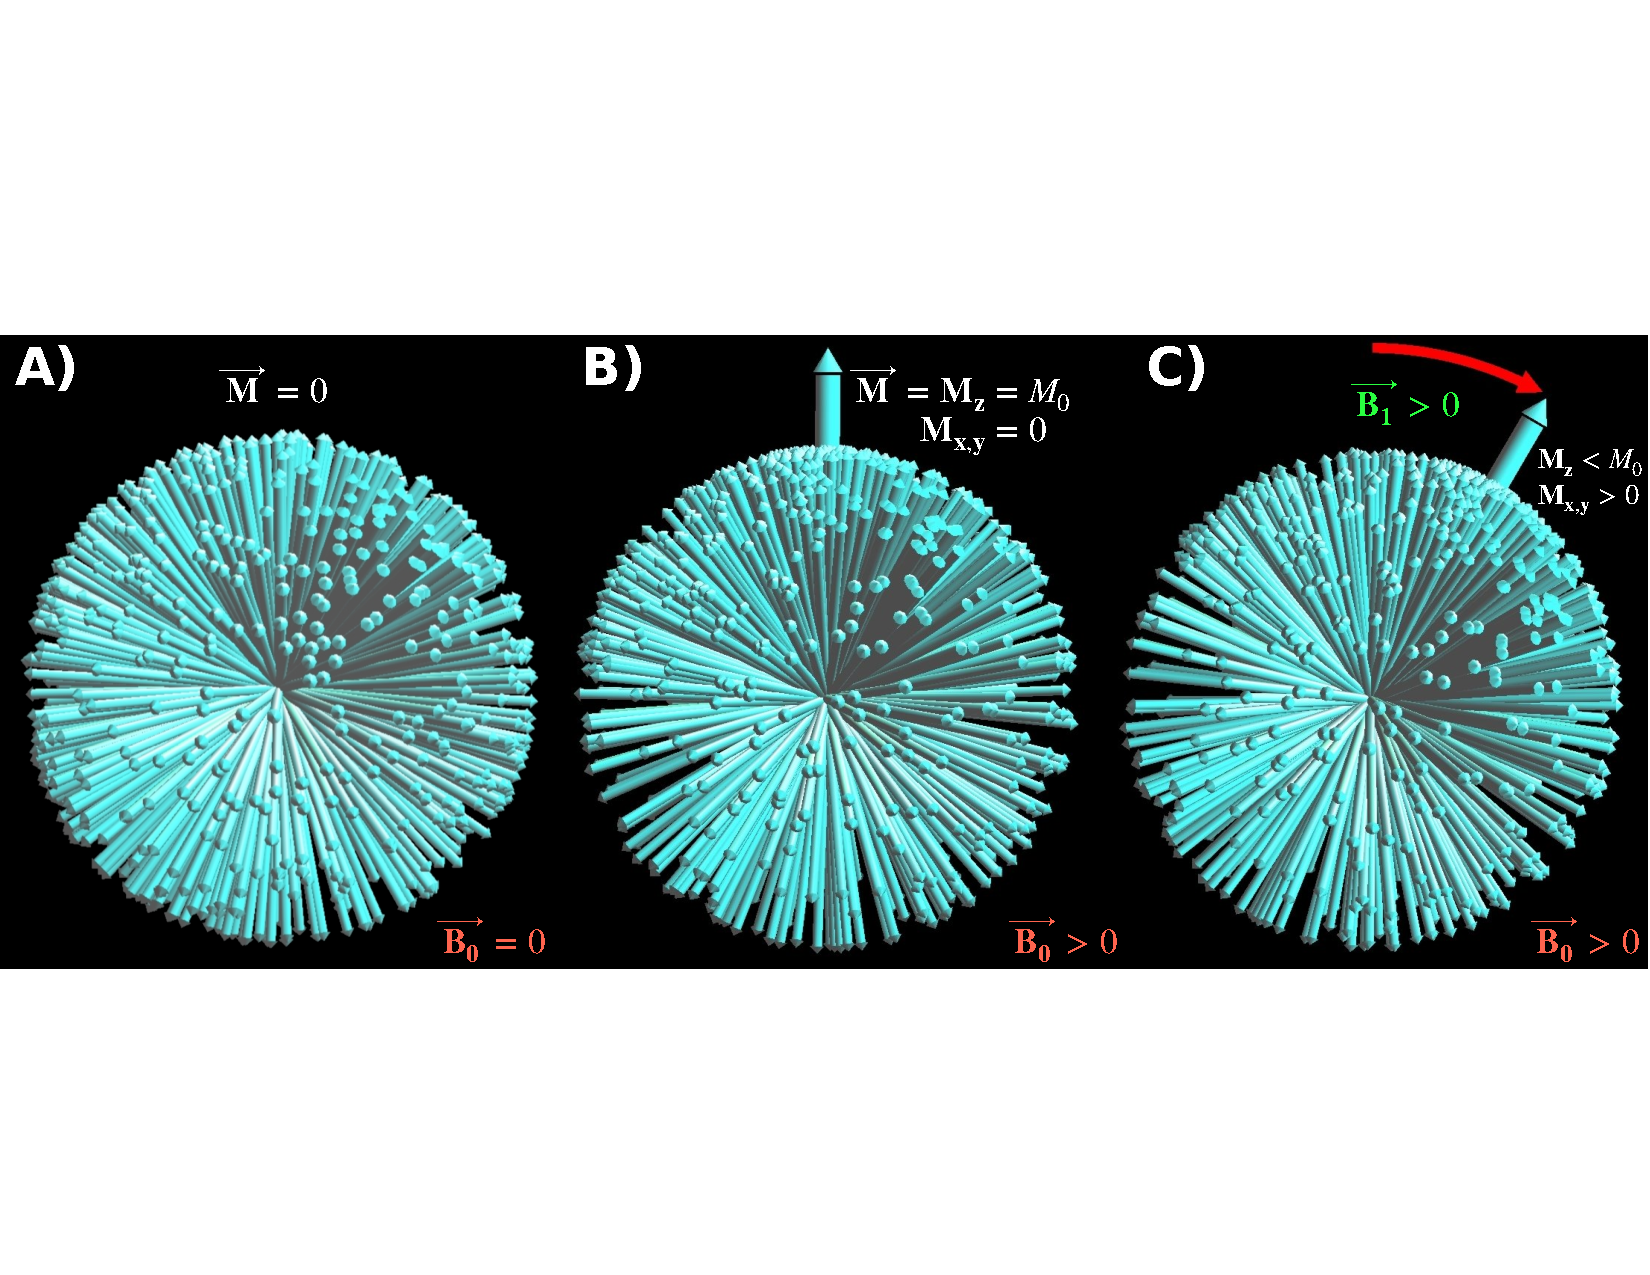
\includegraphics[width=\textwidth]{./intro/intro-images/HansonMRI.pdf}
	\caption[Spins getting tipped with an RF pulse]{The net magnetization vector M$_0$ is tipped to the transverse axis with an RF pulse so the signal can be measured. 
Images used with permission from Hanson et al. 
(\cite{Hanson:2008tp})}
	\label{spinsB0B1}
\end{figure}

Back to the bucket of water, or rather, a collection of many many small bar magnets.
Rather than consider 1$0^{25}$ bar magnets, it is simpler to consider the net magnetic moment of all the protons in aggregate.
This vector is typically referred to as the magnetization vector $\vec{\mathbf{M}}$ and comprises MRI signal and its manipulation and interactions with the surrounding environment ultimately lead to the images produced.
Because the magnets are tumbling around in the bucket of water due to thermal motion, they are pointed in nearly every direction (figure~\ref{spinsB0B1}A) and $\vec{\mathbf{M}} = 0$.
If we now put this bucket of water into an MRI scanner with a main magnetic field strength $\vec{\mathbf{B_0}} = 7$ Tesla, there is a slight tendency of individual protons to align with the main magnetic field $\vec{\mathbf{B}}$ (along z axis, see figure~\ref{spinsB0B1}B).
Consequently the magnetization vector $\vec{\mathbf{M}}$ now aligns with $\vec{\mathbf{B_0}}$.
If $\vec{\mathbf{M}}$ is split into its components (along the x, y, and z axes), the longitudinal magnetization component $\mathbf{M_z} = M_0$ and the transverse magnetization component $\mathbf{M_{x,y}} = 0$.
$\vec{\mathbf{M}}$ is many orders of magnitude smaller than the external magnetic field so the MR signal cannot be measured when it is aligned with the external main magnetic field $\vec{\mathbf{B}}$. 
Applying a radiofrequency (RF) pulse $\vec{\mathbf{B_1}}$ at the Larmor frequency results in a torque applied to $\vec{\mathbf{M}}$, causing it to `tip' down into the transverse (x-y) plane (figure~\ref{spinsB0B1}C)

In the transverse plane, interacting nuclei exchange energy with both the surrounding environment (spin-lattice interaction) as well as neighbouring nuclei (spin-spin interaction), and $\vec{\mathbf{M}}$ relaxes back to its equilibrium value. 
The time it takes for $\mathbf{M_z}$ to return to its equilibrium value $\vec{\mathbf{M_0}}$ from 0, is characterized by the time T$_1$,

\begin{equation}
	M_z = M_z(1-e^{-t/T_1})
	\label{T1}
\end{equation}

Similarly, the transverse magnetization $\mathbf{M_{x,y}}$ decays to 0 through the interactions between nuclei and is characterized by the time T$_2$ (also called spin-spin relaxation).
		
\begin{equation}
		M_{xy} = M_0 e^{-t/T_2}
		\label{T2}
\end{equation}

Although T$_1$ and T$_2$ values are affected by various factors including field-strength, and local environmental factors such as temperature, proton concentration, and molecular mobility. 
Differences in T$_1$ and T$_2$ values are used to generate contrast between different tissues. 
For example in study conducted with ten volunteers at 1.5T, the spleen ($T_1 = 919$ ms), liver ($T_1 = 616$ ms), muscle ($T_1 = 785$ ms), fat ($T_1 = 239$ ms), and renal cortex ($T_1 = 919$ ms) all had measurably different $T_1$ values~\cite{OConnor:2009ku}.
Paramagnetic contrast agents are often used to increase the T$_1$ contrast between different species. 
The following sections outline how dynamic contrast-enhanced MRI or \acs{DCE-MRI} is used in the imaging of cancer.

\subsubsection{Paramagnetic contrast agents}

Paramagnetism is defined as the intrinsic tendency for a material to become magnetized when placed within a magnetic field.
By far the most common element used as a contrast agent (tracer) in MRI is Gadolinium as it is strongly paramagnetic due to its seven unpaired electrons.
Because electrons are much smaller than protons but have the spins, they have a significantly higher gyromagnetic ratio.
The unbalanced electrons in the gadolinium shell or bonding orbital results in a strong net magnetic moment, which interacts with hydrogen nuclei and dramatically reduces the longitudinal relaxation time T$_1$ (and to a lesser extent T$_2$).
Unfortunately free metal ions are poorly tolerated by the body so the Gadolinium ions need to be attached to an organic chelating agent~\cite{DeLeonRodriguez:2015bl}.

The ability for a contrast agent to affect the T$_1$ relaxation time is given by its relaxivity $r_1$, obtained from the following equation:

\begin{equation}
\frac{1}{T_{1}} = \frac{1}{T_{1_0}} + r_1 [Gd]
\end{equation}

where T$_{1_o}$ is the initial T$_1$, prior to the influence of the paramagnetic contrast agent, $r_1$ is the relaxivity of the contrast agent in units of $(mM\cdot)^{-1}$, and $[Gd]$ is the contrast agent concentration.
It is important to note that all contrast agents shorten both T$_1$ and T$_2$ but whether their dominant influence is on the transverse relaxation time (T$_2$) or the longitudinal relaxation time (T$_1$) depends on the relative strengths of $r_1$ and $r_2$.

\subsubsection{Dynamic contrast-enhanced MRI (\acs{DCE-MRI})}

\acs{DCE-MRI}) is a tremendously useful to increase contrast between species whose T$_1$ and T$_2$ times are similar.
However the true value of \acs{DCE-MRI} comes from extracting physiologically relevant information from the body. 
In applications of cancer imaging, \acs{DCE-MRI} has been extremely successful in diagnostics, treatment monitoring, assessing severity of pathologies, distingushing between tumour models and types, improving our understanding of tumour metastases, and development of drugs.\todo[backgroundcolor=red!20!white]{add a reference to each of these}

Health Canada has approved several gadolinium-based contrast agents for use in humans and one common one is \acs{Gd-DTPA} - a gadolinium ion chelated to an organic ligand DTPA.
\acs{Gd-DTPA} is a small molecule that readily traverses the endothelium but not the cell membrane~\cite{WalkerSamuel:2006ch}. 
This property allows modeling of the vascular dynamics of the tumour but because the contrast agent is small, perfusion and permeability cannot be decoupled.
Choosing a kinetic model to fit the data requires some prior knowledge about the organ or system in question. 
For instance, the blood-brain barrier in the dramatically alters the contrast agent kinetics. 
Similarly, in leaky tumours the extravascular contrast agents typically used in \acs{DCE-MRI} leak out (and back in) of vasculature considerably faster than in other tissues. 
Sourbron et al. indicate that choice of a tracer kinetic model should provide a link between relevant physiological parameters and measured data~\cite{Sourbron:2011ce}. 

The most widely used model in \acs{DCE-MRI} is the extended Toft's model, which is valid in highly perfused tissues and weakly vascularized tissues with a well-mixed extravascular extracellular space ($v_e$)~\cite{Sourbron:2013jz}.
Figure~\ref{XTofts} provides a graphical description of this two compartment model,and its mathematical representation is:

\begin{equation}
C(t) = v_p \cdot AIF(t) + K^{trans}e^{-t\frac{K^{trans}}{v_e}} * AIF(t)
\end{equation}

where \acs{$v_p$} is the plasma volume, \acs{K$^{trans}$} is the volume transfer constant, and the \acs{AIF}(t) is the arterial input function which needs to be measured independently of the contrast agent kinetics.


\begin{figure}[htbp]
   \centering
   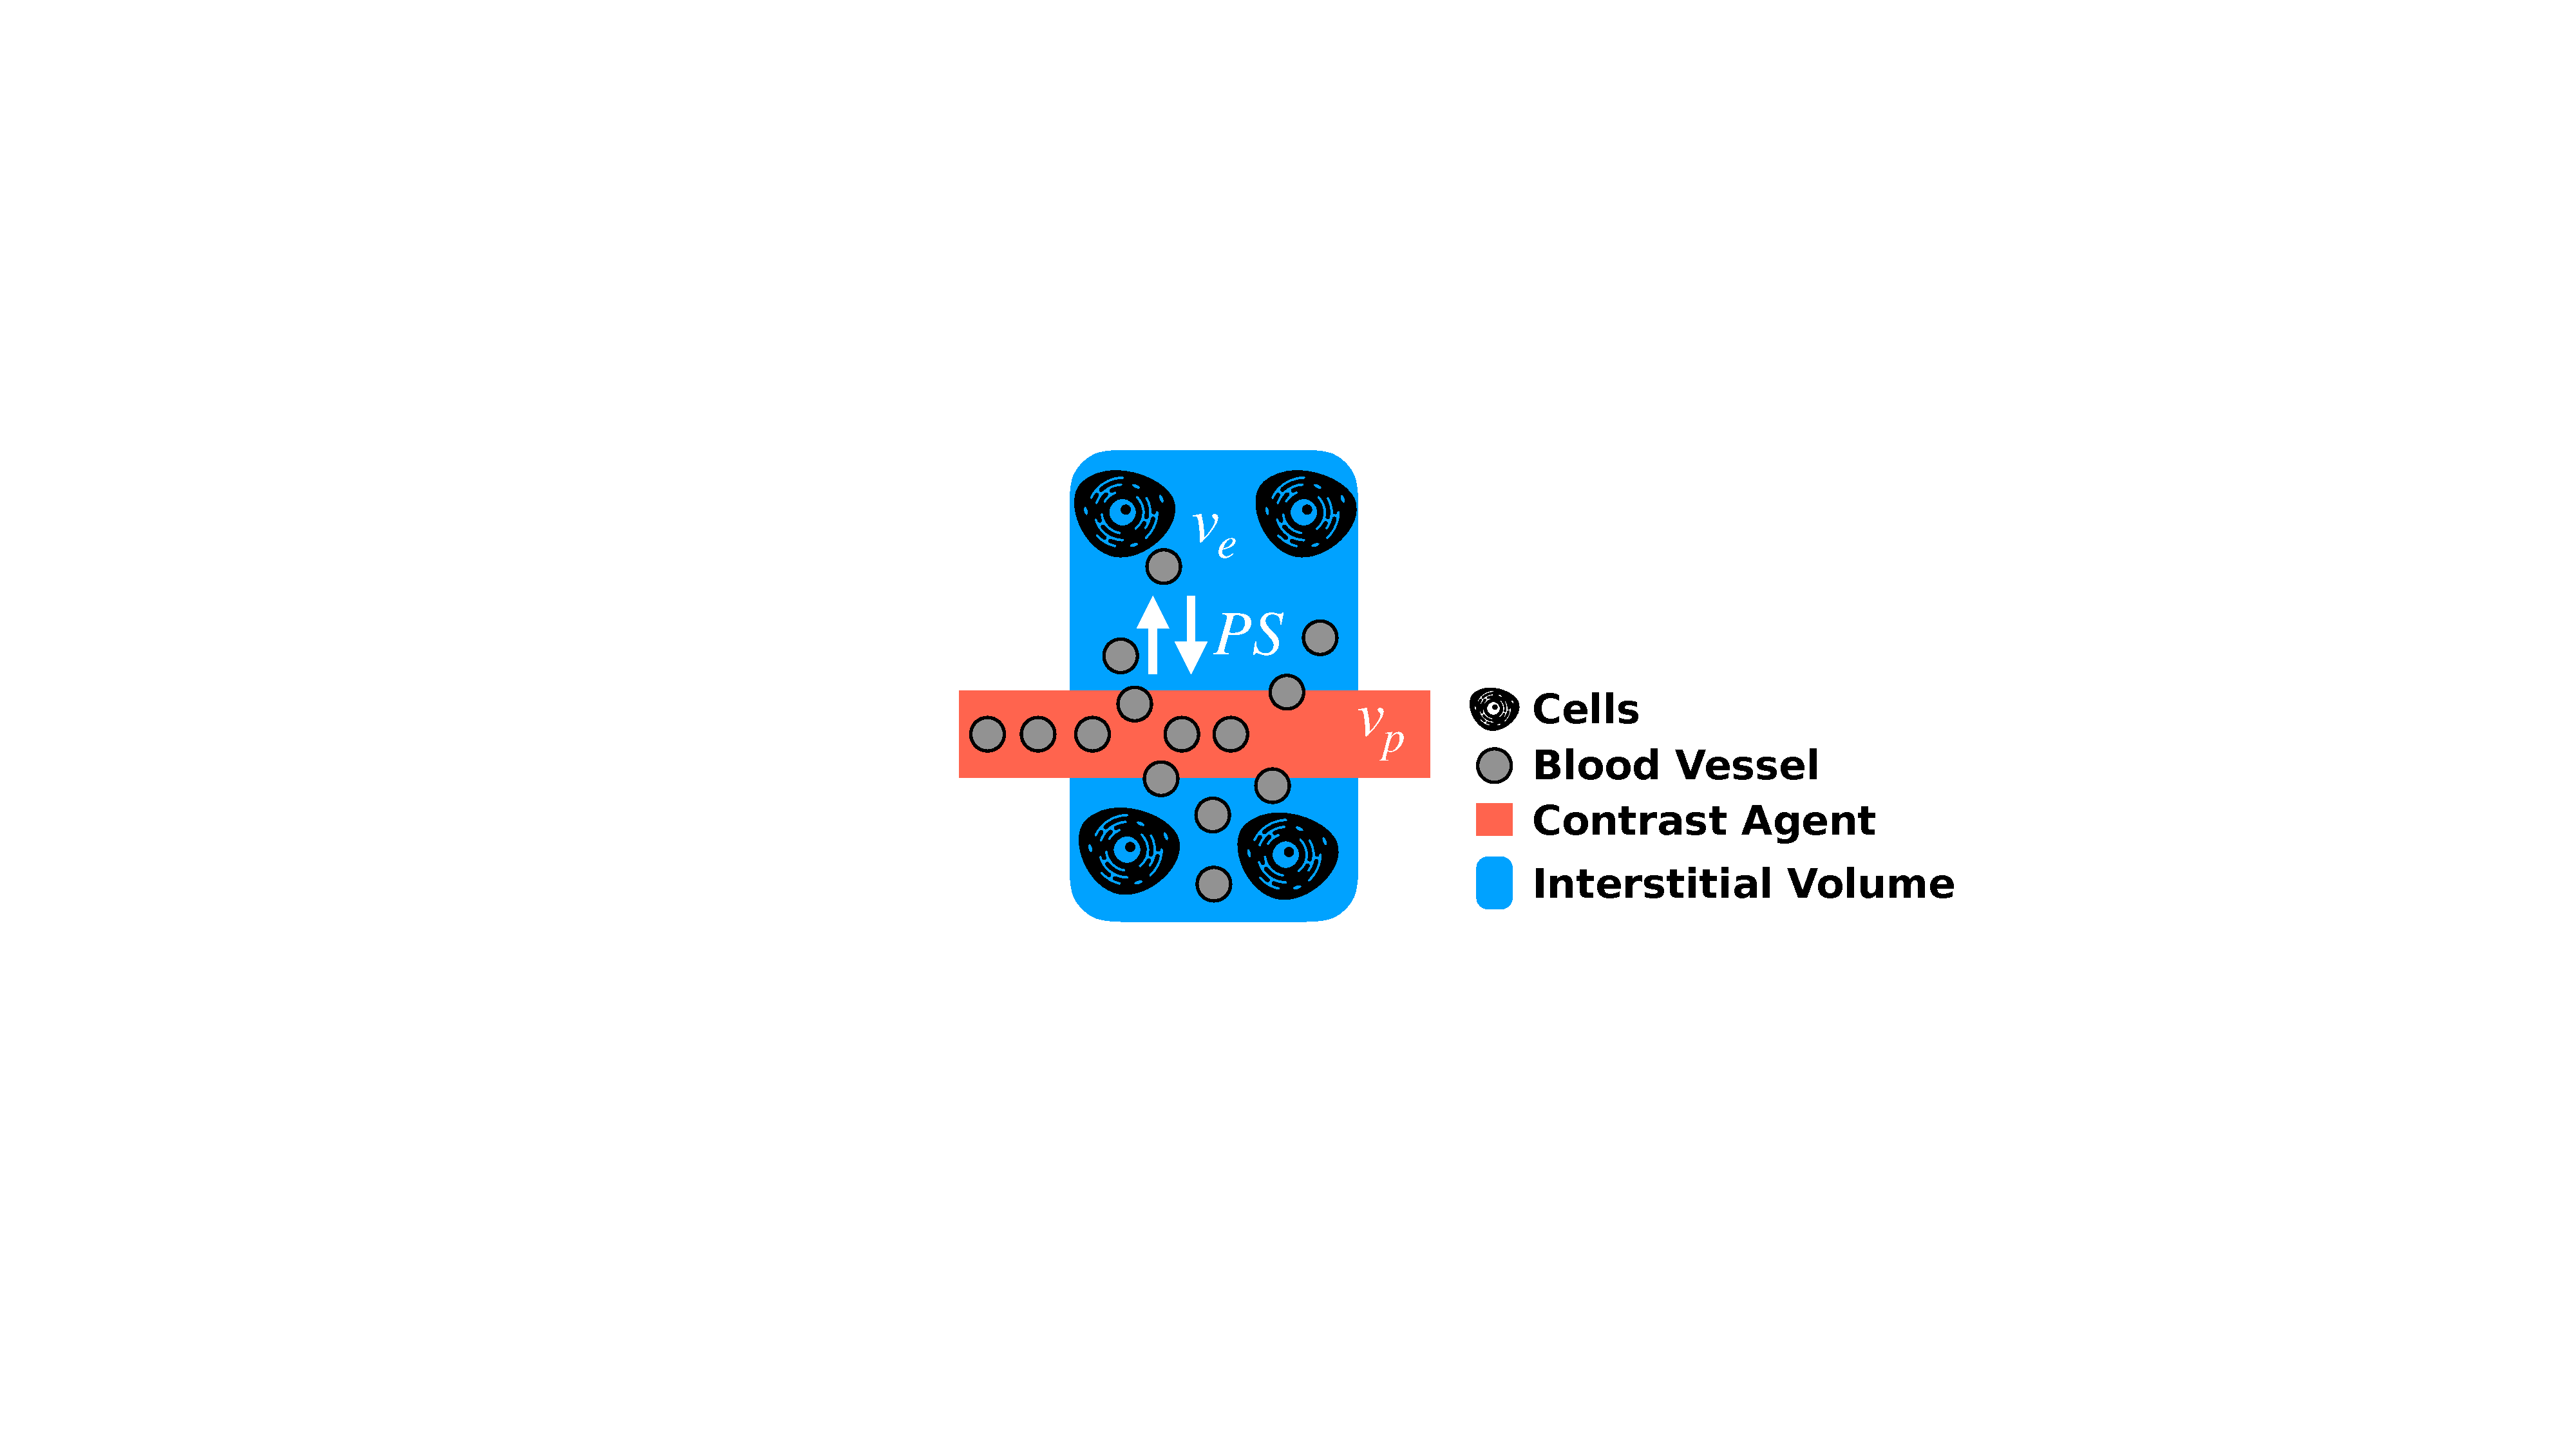
\includegraphics[width=\textwidth]{intro/intro-images/XTofts.pdf}
   \caption[Extended Tofts Model]{Graphical description of the Extended Tofts Model. An arterial input function (\acs{AIF}) governs the introduction of the tracer (grey circles) in the vascular compartment (pink) via a bolus injection. Contrast agent molecules exchanges with the extravascular extracellular space (\acs{$v_e$}, interstitial volume in blue) at a rate given by $PS$, the permeability-surface area product.}
   \label{XTofts}
\end{figure}

Thus, modelling of \acs{DCE-MRI} data to produce quantitative and physiologically relevant values of \acs{K$^{trans}$}, \acs{$v_p$} and \acs{$v_e$} requires an accurate calculation of the \acs{AIF}.
In this thesis, \acs{DCE-MRI} modelling using a traditional small molecule agent (\acs{Gd-DTPA} is used only briefly in Chapter~\ref{ch:HPG} and the \acs{AIF} used in that modelling was measured and published by a former lab member~\cite{Moroz:2013ee}.
Nevertheless, the concepts and introduction to \acs{DCE-MRI} are relevant for several portions of the thesis. 

\section{Thesis structure}

In Chapter~\ref{ch:HPG} we begin by describing a new macromolecular contrast agent and explore its value in describing the tumour microenvironment.
A two-parameter linear model was applied to the contrast agent enhancement curve and we obtained measures of vessel permeability and fractional plasma volume.
These parameters were then used to distinguish between two tumour models.
In Chapter~\ref{ch:HPG2}, we applied this technique to determine whether molecule size played a role in the distribution of a high molecular weight anti-cancer drug (Trastuzumab).
Ultimately we showed that neither vessel permeability nor fractional plasma volume corresponded to presence of bound drug (determined via histological staining), suggesting other barriers that limit distribution of Trastuzumab.
In Chapter~\ref{ch:HPG3} we considered another application of the new contrast agent: can we assess changes in vessel permeability after administering an anti-angiogenic drug?
We discovered that vessel permeability is indeed reduced after drug treatment but along the way we also showed that histologically, hypoxia dramatically decreased after treatment. 
This led us along the journey to develop a new method to assess tumour oxygenation~\emph{in vivo} using MRI and a brief interlude is inserted here to provide some more background information about oxygen and related physiology.
Chapter~\ref{ch:oemri} outlines our technique and describes the use of a blind source separation technique to increase the sensitivity of existing methods. 
We validated the technique in Chapter~\ref{ch:oemri2} with histological staining, and demonstrated utility of a new parameter to separate oxygenation replenishment in different tumour models.
Finally in Chapter~\ref{ch:oemri3} we showcase a typical application of the technique: detection of tumour oxygenation improvements after administering an anti-angiogenic agent. 
We also showed that the tumour implant site has a large bearing on the tumour microenvironment, and no oxygenation improvements are observed if the baseline oxygenation is high.
In Chapter~\ref{ch:futurework} some interesting observations are presented that may be useful starting points for future work in this field.

%    2. Main body
% Generally recommended to put each chapter into a separate file
%% The following is a directive for TeXShop to indicate the main file
%!TEX root = ../diss.tex

\chapter[MRI and histology of vascular function in xenografts using \acs{HPG-GdF}]{Multi-modal magnetic resonance imaging and histology of vascular function in xenografts using macromolecular contrast agent hyperbranched polyglycerol (HPG-GdF)}
\label{ch:HPG}

\section{Introduction}
The vascular network in tumour tissue is abnormal, often resulting in vessels that have variable flow rates and high permeability relative to blood vessels in normal tissue~\cite{McDonald:2002ut}.
Dynamic contrast enhanced magnetic resonance imaging (DCE-MRI) is a useful tool for non-invasively assessing tumour vasculature by imaging and measuring concentrations of \acs{CA} delivered to tumours by the vessels~\cite{OConnor:2012ie,Barrett:2006jx,Leach:2003fy}. \todo[backgroundcolor=blue]{I couldn't search well to confirm this is the first case of the abbrv on this app. Assuming chp 2 is the start - define first}
The appeal of a dynamic, non-invasive approach for measuring tumour vascular function in the clinic is clear.
Such data is applicable in the field of assessing treatment response for vascular targeting therapies~\cite{OConnor:2012ie,Barrett:2006jx,Leach:2003fy}.
In addition to utility as a treatment biomarker, vascular function data may be able to predict which tumours are likely to respond to therapy~\cite{DeBruyne:2012cq,Kelly:2011cf,Bains:2009hh}, or which regions or tumours have greater heterogeneity in their microenvironment~\cite{OConnor:2011jm,Alic:2011hw}.
The issue of limited access for anticancer drugs in solid tumours is significant~\cite{Minchinton:2006gs}, particularly given the efforts to create nanoparticle therapeutics that target the tumour via \acs{EPR} effect~\cite{Jain:2001uf,Iyer:2006gf,Chauhan:2011fi}.
A translatable imaging protocol and suitable contrast agent that yields meaningful, reproducible biomarkers of vascular function could be widely useful in these areas of cancer research.

Low \acs{MW} Gd(III)-based, chelated \acs{CA}s such as Gadovist (MW = 605 Da) exhibit short half-lives and rapid renal clearance~\cite{Weinmann:1984gv}.
With the exception of brain tissue containing a functional blood-brain barrier, low MW Gd agents currently in clinical use diffuse across the vascular endothelium in most normal and neoplastic tissues.
Therefore, a well-established shortcoming of low MW contrast agents is the difficulty of attributing local signal enhancement specifically to either vascular perfusion or vessel permeability.
The ability to characterize physiologically relevant biomarkers of vascular function is desirable for studying the effects of anti-angiogenic treatments in tumours (described in a comprehensive review regarding DCE-MRI and anti-vascular therapies in cancer~\cite{OConnor:2012ie}).
Development and application of macromolecular contrast agents (MCAs) attempt to improve upon DCE-MRI assessment of vascular function by relying on the primarily intravascular nature of \acs{MCA}s.
High MW contrast agents and therapeutics unable to diffuse across the endothelium selectively extravasate from large pores and inter-endothelial cell gaps that characterize the abnormal vessels in the tumour microenvironment~\cite{McDonald:2002ut,Hashizume:2000bq}.
MCAs commonly used in cancer research include albumin, dextran polymers, and PAMAM or PPI dendrimers conjugated with DTPA/DOTA-Gd3+ chelates as described by Tang et al.~\cite{Tang:2013fi}.
The size of \acs{MCA}s in use or under development ranges considerably, but may be as small as a 90 kDa albumin conjugate, or one of a range of dextran sizes~\cite{Barrett:2006jx}.
Particles less than 5 nm in size have been found to leak rapidly from tumour vasculature, whereas those in the 5-8nm range are limited to leaking from hyperpermeable vessels; those greater than 8nm are thought to have minimal leakage~\cite{Kobayashi:2004vq,Sato:2001tt}.
The most commonly used \acs{MCA}s in preclinical research are albumin based; however, these are not translatable to the clinic due to immunogenicity concerns~\cite{Ogan:1987tg}.
Signal enhancement is linked to contrast agent concentration within the tumour blood vessels at early time points after injection for \acs{MCA}s that remain intravascular, such that tumour plasma volumes (Vp) can be determined.
Rates of \acs{MCA} leakage from hyperpermeable vessels may then be modeled to evaluate permeability, since extravascular accumulation of the agents will manifest as increased enhancement in repeat images~\cite{Ogan:1987tg,Turetschek:2004bw}.
This analysis is dependent on the assumption that the \acs{MCA}s have unidirectional flow and do not leak back into the plasma, and that the concentration in the plasma is constant, creating a permeabilitylimited environment.
In this study we investigated a multi-modal, high MW contrast agent, \acs{HPG-GdF}: hyperbranched polyglycerol (HPG) molecules doubly labeled with Gd-DOTA and a fluorescent marker.
HPGs are soluble, globular, asymmetrical, have low immunogenicity and are highly biocompatible molecules with low polydispersity~\cite{Saatchi:2012hc,Kainthan:2006ce,Saatchi:2012gc}.
HPG has been previously tested as a human serum substitute~\cite{Kainthan:2008ek} and as a drug delivery vehicle due to its versatility as a chemical, such that drugs, Gd chelates, fluorescent and radiolabels may all be attached to it~\cite{Shenoi:2013id}.
Many other \acs{MCA}s, including Gd-albumin, are highly viscous, which can limit the applicable dose~\cite{Imranulhaq:2012ij}.
The MW of \acs{HPG-GdF} is tunable to required applications, and a biodegradable version of HPG is also available for potential use~\cite{Shenoi:2013id}.
The \acs{HPG-GdF} described in this study is 583kDa and 8-10nm in diameter; synthesis of \acs{HPG-GdF} has previously been described~\cite{Saatchi:2012hc}.
A significant advantage of \acs{HPG-GdF} is that it is a multi-modal agent, with both fluorescent and Gd-chelate labels that permit histological validation of observations made using MRI, including determining the degree to which the agent extravasates from the vasculature.
Previous studies have also used 111In as a SPECT label with utility for biodistribution studies~\cite{Saatchi:2012hc}.
In this work, we employed comprehensive histological methods to investigate the microregional location of \acs{HPG-GdF} in two human colorectal xenograft models, and used this information to interrogate observations made non-invasively using DCE-MR imaging of the same agent in the same tumours.

\section{Methods}

\subsection{Mice and tumours}

Female NOD/SCID mice were bred and housed in institutional animal facilities; experiments in this study were approved by the Animal Care Committee of the University of British Columbia.
Fiducial markers were constructed of PE-50 polyethylene tubing (inner diameter, 0.58mm) and filled with paraffin wax and saline, creating an MR-visible interface~\cite{Bains:2009hh}.
Marker tubes were implanted subcutaneously in the sacral region of mice, in a craniocaudal orientation, 2 days prior to subcutaneous implantation of tumours.
Both histological and MR modalities imaged slices in the plane perpendicular to the marker tube to minimize angular differences between serial MR image slices obtained over multiple sessions, and for corresponding cryosections in histological processing.
HCT116 or HT29 human colorectal carcinoma cells obtained from the American Type Culture Collection (ATCC) were implanted near the fiducial tubes such that the tumours grew around the tubes.
Tumours were used when diameters reached 8-12 mm.
Mice were anaesthetized with isoflurane for the duration of imaging sessions.
Animals were positioned supine on the custom surface coil apparatus fitted with a lid lined by a temperature-controlled, water-filled heating blanket.
Body temperature and respiration rate were monitored throughout imaging.
Following their final scan animals were administered a 35 $\mu$L intravenous dose of 0.6 mg/mL carbocyanine (DioC7(3); Molecular Probes, Eugene, OR, USA) in 75\% dimethylsulfoxide as a fluorescent dye indicator of vessel perfusion in histological measures, and euthanized 5min after injection.
Some animals received \acs{HPG-GdF} and tumours were collected at early time points for histological analysis only, with no MR-imaging.
Tumors were embedded and frozen vertically in optimum cutting temperature medium (OCT; Tissue-TEK) using their fiducial markers for guidance.

\subsection{Contrast agents and dosage}

Hyperbranched polyglycerol (HPG-GdF) (Fig.~\ref{hpgpaper1:fig1}): 583 kDa HPG was synthesized at the University of British Columbia (D. Brook’s laboratory, Department of Chemistry) with a narrow polydispersity of PDI = 1.01 by ring-opening multibranching polymerization of glycidol using dioxane as the reaction medium, according to a published procedure~\cite{Kainthan:2006ce}.
HPG was derivatized with p-NH2-benzyl-DOTA (Macrocyclics, Dallas, TX, USA) at 20$\mu$g Gd per mg HPG and tagged with Alexa Fluor 647 (Invitrogen Life Technologies, Burlington, ON, Canada) as previously described (20).
The biological half-life of HPG-Gd (with no fluorescent tag) in mice has previously been examined in biodistribution studies and was reported as 32.6 h (20).
HPG-GdF was administered as a 6 $\mu$L/g bolus dose from 100 mg/mL (0.2 mM) using an intravenous (i.v.) catheter; therefore, the administered molar dose of HPG was 1.2 nmol/g and that of the chelated Gd(III) was 240-360 nmol/g (determined according to an estimated 200-300 chelates per HPG molecule (20)).
Assuming a blood volume of 5\% of mouse body weight, peak blood concentration of \acs{HPG-GdF} is 24$\mu$M.
This value has been used to normalize relative tissue concentrations (Fig.~\ref{hpgpaper1:fig2}(B)) and to calculate the fractional plasma volume (fPV; see Section 2.4).
The relaxivity of \acs{HPG-GdF} has previously been measured and reported to be 1075 mM$^{-1}$s$^{-1}$1, which is approximately 300 times greater than that of Gadovist (3.58 mM$^{-1}$1 s$^{-1}$1) (20).
Gadovist (Bayer Healthcare, Toronto, ON, Canada; 607.4 Da) was administered by i.v. catheter as a 5 $\mu$L/g bolus dose from 60 mM solution, for an administered molar dose of Gadovist of 300 nmol/g.
All in-scanner i.v. injections were performed using a power injector at a rate of 1 mL/min.
An extended fluid line connected to the i.v. catheter secured to the tail vein of the mice permitted remote initiation of injections outside the scanner room.
Injections included a small volume (<40 $\mu$L) of heparinized saline followed by the contrast agent, which was then followed by a 20 $\mu$L flush of heparinized saline.

\begin{figure}[htbp]
 \begin{center}
 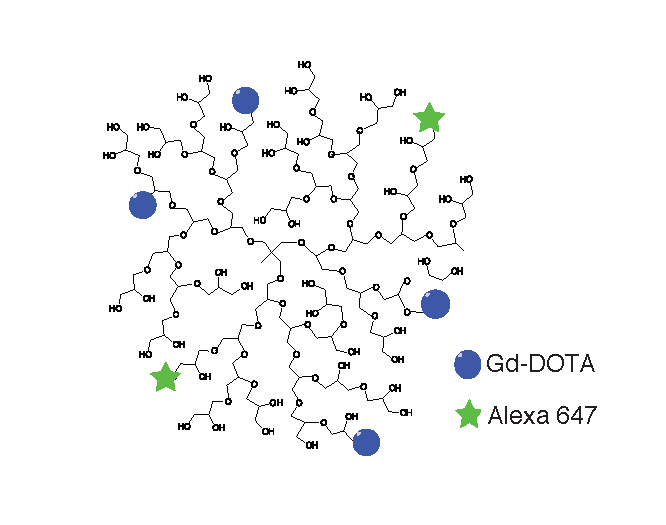
\includegraphics[width=\textwidth]{hpg/hpg-paper1-images/hpg_fig1-hpgdf.pdf}
 \caption{HPG-GdF. The 583 kDa globular Hyperbranched PolyGlycerol (HPG) molecules are derivatized with p-NH$_2$-benzyl-DOTA (Macrocyclics) at 20 $\mu$g Gd per mg HPG (approximately 300 chelates per molecule) and tagged with Alexa Fluor 647 dye, as previously described (\cite{Saatchi:2012hc}.}
 \label{hpgpaper1:fig1}
 \end{center}
\end{figure}

\subsection{MRI acquisition}

All MRI experiments were performed at the UBC MRI Research Centre on a 7T Bruker BioSpec 70/30 scanner at room temperature with a combination of volume (transmit)/surface (receive) coil.
Each imaging session began with axial RARE T$_2$-weighted images for morphological reference and precise alignment of imaging plane.
Further T$_1$-weighted RARE images were acquired for qualitative assessment of contrast agent distribution.
During the first scanning session, T$_1$ and flip angle maps were acquired prior to a DCE-MRI experiment, followed by another T$_1$ measurement.
At each imaging session slice location and orientation were adjusted to match previous sessions.
T$_1$ measurements and flip angle mapping were performed using a multi-slice FLASH variable flip angle experiment (FLASH TR/TE = 500/2.75, FA = 10$^{\circ}$, 20$^{\circ}$, 30$^{\circ}$, 40$^{\circ}$, 50$^{\circ}$, 60$^{\circ}$, 70$^{\circ}$, 80$^{\circ}$, 90$^{\circ}$, 100$^{\circ}$, 110$^{\circ}$, 120$^{\circ}$, 130$^{\circ}$, 140$^{\circ}$, 150$^{\circ}$, 160$^{\circ}$, 170$^{\circ}$, 180$^{\circ}$, 190$^{\circ}$, 200$^{\circ}$, 215$^{\circ}$) and data were fit simultaneously for T$_1$ and the B1 scaling factor map.
DCE-MRI data was collected at 2.24 s time resolution (FLASH; TR/TE = 35/2.75; FA = 40; NR = 1200).
T$_1$ and DCE-MRI experiments all had identical geometry (matrix = 128 x 64; three slices; voxel size = 0.33 mm x 0.297 mm x 1.5 mm; 2.5 mm slice separation).
A follow-up T$_1$ measurement was performed (FLASH; TR/TE = 35/2.75; FA = 10$^{\circ}$, 20$^{\circ}$, 30$^{\circ}$, 40$^{\circ}$, 50$^{\circ}$, 60$^{\circ}$, 80$^{\circ}$, 100$^{\circ}$, 120$^{\circ}$) and the B$_1$ scaling factor map from the baseline acquisition was used to determine post-contrast T$_1$ (assuming that B$_1$ scaling does not change due to contrast injection).
Difference maps of relaxation rates $\delta$R$_1$ = 1/T$_1$(post-contrast) - 1/T$_1$(precontrast) were constructed for a measure of contrast agent concentration.
Animals received two DCE-MRI scans 24-48h apart, with Gadovist administered and scanned at the first session and \acs{HPG-GdF} administered and scanned at the subsequent session with tumours collected for histological processing at about 60 min post administration of their \acs{HPG-GdF}.

\begin{figure}[htbp]
 \begin{center}
 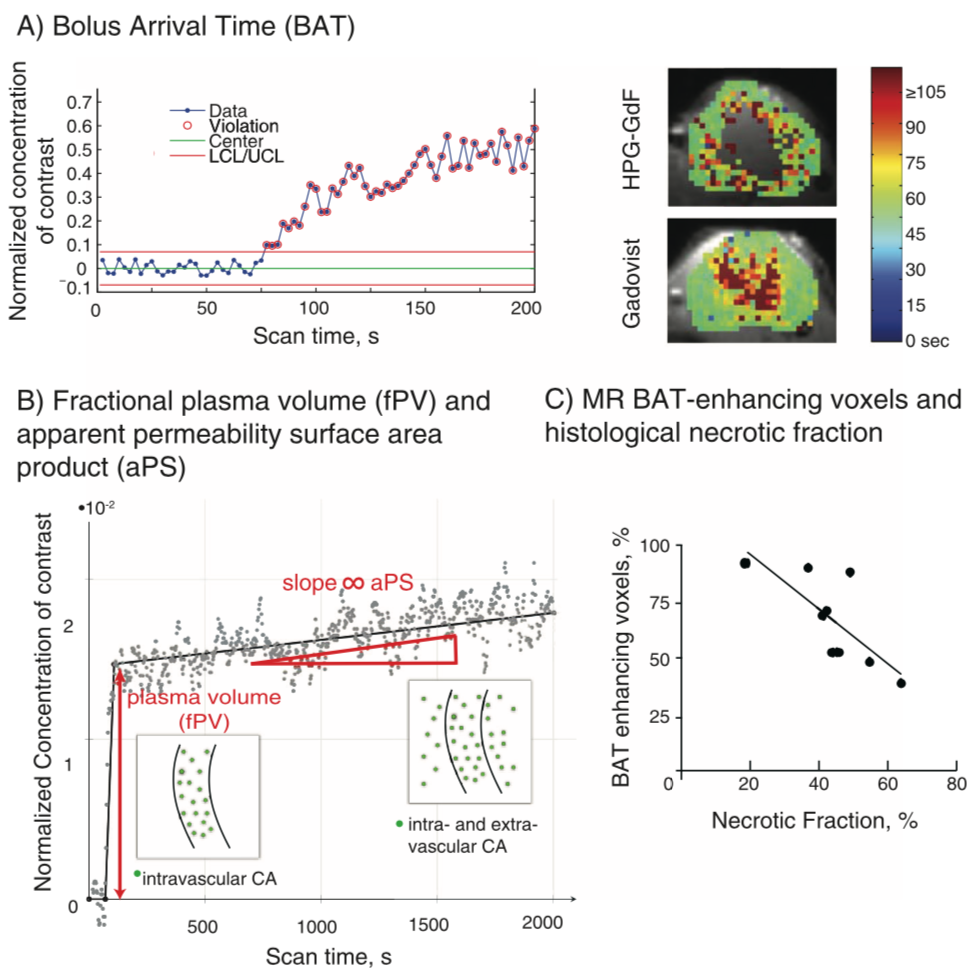
\includegraphics[width=\textwidth]{hpg/hpg-paper1-images/hpg_fig2-bat.png}
 \caption{MR-derived parameters to measure vascular function using \acs{HPG-GdF}: bolus arrival time (BAT), fractional plasma volume (fPV) and apparent permeability-surface area product (aPS). (A) Sample curve showing change in concentration of \acs{CA} as a function of scan time. The first violation (circle) is identified by Rule (1) at Frame 31, corresponding to a BAT of t = 77.5 s. The centre (mean) and upper (UCL) and lower (LCL) control limits ($\pm$3 SDs) are drawn for reference. Sample BAT parameter maps from \acs{HPG-GdF} and Gadovist obtained from the same HT29 xenograft imaged 24h apart show that \acs{HPG-GdF} is slower to arrive; both \acs{CA}s arrive most quickly at the tumour margins. (B) \acs{HPG-GdF} enhancement curve shown for a full imaging period where the bolus arrival is seen as a significant jump in enhancement from which the \acs{fPV} is derived as the concentration at the start relative to the plasma concentration, since the \acs{CA} is largely intravascular at that early time. The \acs{aPS} is the slope of the enhancement after the bolus arrival. The concentration curves are shown as ratio of tissue concentration to blood peak concentration (24 $\mu$M) (C) The fraction of MR-measured \acs{HPG-GdF} BAT-enhancing voxels has a negative association with the proportion of necrotic tissue determined in histological sections.}
 \label{hpgpaper1:fig2}
 \end{center}
\end{figure}

\subsection{MRI data analysis}

Regions of interest (ROIs) were drawn on T2-weighted RARE images to outline the tumour using ImageJ (NIH), and all other MR analysis was performed using MATLAB (MathWorks, R2009a) and Python.
T$_1$ and flip-angle maps were calculated from variable flip-angle data with a slice-profile correction based on simulations described by Parker et al.~\cite{Parker:2001wj}.
The same method was extended to provide time-dependent T$_1$ and concentration-time in DCE data series.
Areas under the curves (AUCs) were numerically integrated starting from the bolus arrival time, or, for tumour-averaged AUC, starting from the common injection time point and extended to the indicated time points (1 and 37 min).
Bolus arrival time (BAT) is the time when detectable signal enhancement begins for a voxel (Fig.~\ref{hpgpaper1:fig2}(A)) due to contrast agent arrival.
Based on the control-chart decision criterion and the Western Electric decision rules from MATLAB’s statistical toolbox~\cite{Shewhart:1931tq}, voxel enhancement was detected as a positive change from baseline signal for three consecutive timepoints (frames) (i) in the same direction, (ii) starting 5 s before the time of injection or later and (iii) for at least 10\% of all timepoints following initial change of signal away from baseline.
Therefore, voxels with a finite BAT and for which at least 10\% of the following intensities were classified as enhancing by the BAT criteria were called enhancing voxels, whereas all other voxels were labeled as non-enhancing.

A change from baseline was determined to have occurred
when any one of the following inclusion criteria were met:

\begin{enumerate}
	\item any point fell outside of 3 SDs from the average baseline concentration, or
	\item two of three consecutive points fell outside of the 2 SD limit on the same side of the mean, or
	\item four of five consecutive points fell outside of the 1 SD line, on the same side of the centre line, or
	\item eight consecutive points all fell on one side of the centre line.
\end{enumerate}

In the illustrated example (Fig.~\ref{hpgpaper1:fig2}(A)), a change from the mean was identified at Frame 31 and the two following scans by Rule (1); therefore, the BAT point was selected as Frame 30.
The centre line (mean of baseline) and upper and lower control limits ($\pm$3 SDs) are drawn for reference.

\subsubsection{Pharmacokinetic modeling of DCE-MRI data}

\textit{Gadovist.} The extended Tofts model was used and three parameters resulted: K${trans}$, vE, and vP~\cite{Sourbron:2011ce}.
The arterial input function (AIF) for this model was determined previously by our laboratory using a projection-based method~\cite{Moroz:2013ee}.
\textit{HPG-GdF.} A two-parameter linear model was applied~\cite{Pathak:2005gu}.
Two parameters were used to characterize the \acs{MCA} time curves: (1) the rapid increase at the time of injection (related to the \acs{fPV}) and (2) the slope of the later enhancement (aPS) (Fig.~\ref{hpgpaper1:fig2}(B)).
The relative plasma volume could be determined from the ratio of concentrations in the voxel of interest to the concentration in whole blood in the seconds after injection, since extra-vascular spread of the agent was negligible at this time.
The slope of the concentration time curve following contrast arrival is proportional to the permeability-surface area product (PS) when the assumption of a permeability-limited environment is valid.
However, in the highly variable tumour microenvironment, extravasation of contrast agent may deplete the intra-vascular concentration appreciably in conditions of high permeability, which would increase the relative contribution of perfusion to the composite measure of PS.
To stress that the interpretation of this slope value depends on the assumption of a permeability-limited environment, we term the slope the apparent permeability-surface area product (aPS)~\cite{DaldrupLink:2004gy,Dafni:2002kb}.

\subsection{Histology}

Cryosections of 10 $\mu$m were obtained along the plane perpendicular to the fiducial marker at depths corresponding to MR imaged slices.
Sections were imaged for DiOC7(3) and HPGGdF native fluorescence and fixed in acetone-methanol for 10min prior to staining and re-imaging for CD31 (PECAM/ CD31) and Hoechst 3342, labeling vascular endothelium and cell nuclei, respectively.
Sections were imaged as previously described~\cite{Kyle:2007ch} using a system of tiling adjacent microscope fields of view such that images of entire tumour cryosections were captured at a resolution of 1.5 $\mu$m/pixel.
Using both fiducial and anatomical landmarks, histological sections were chosen to match the MR slices.
Using ImageJ~\cite{Collins:2007jr} and user-supplied algorithms, digital images were superimposed and manually cropped to tumour tissue boundaries; staining artifacts and necrosis were also removed for some analyses.
Positive fluorescence for CD31 and DiOC7(3) images was obtained by applying a threshold, with neighboring positive pixels grouped as ``objects''.
The average distance of tissue to the nearest vascular object was reported as a repeatable measure of vascular density.
Perfused vessel fraction (PF) was calculated as the proportion of CD31-positive objects that had at least 20\% overlap with positive DiOC7(3) or \acs{HPG-GdF} pixels on the overlaid image.
Data for individual tumours were displayed as mean $\pm$ SEM values.
HPG-GdF extravasation was assessed by its distance from blood vessels: pixels from the \acs{HPG-GdF} fluorescence image were sorted according to their distance from vascular objects and the average \acs{HPG-GdF} fluorescence intensity was reported.

\begin{figure}[htbp]
 \begin{center}
 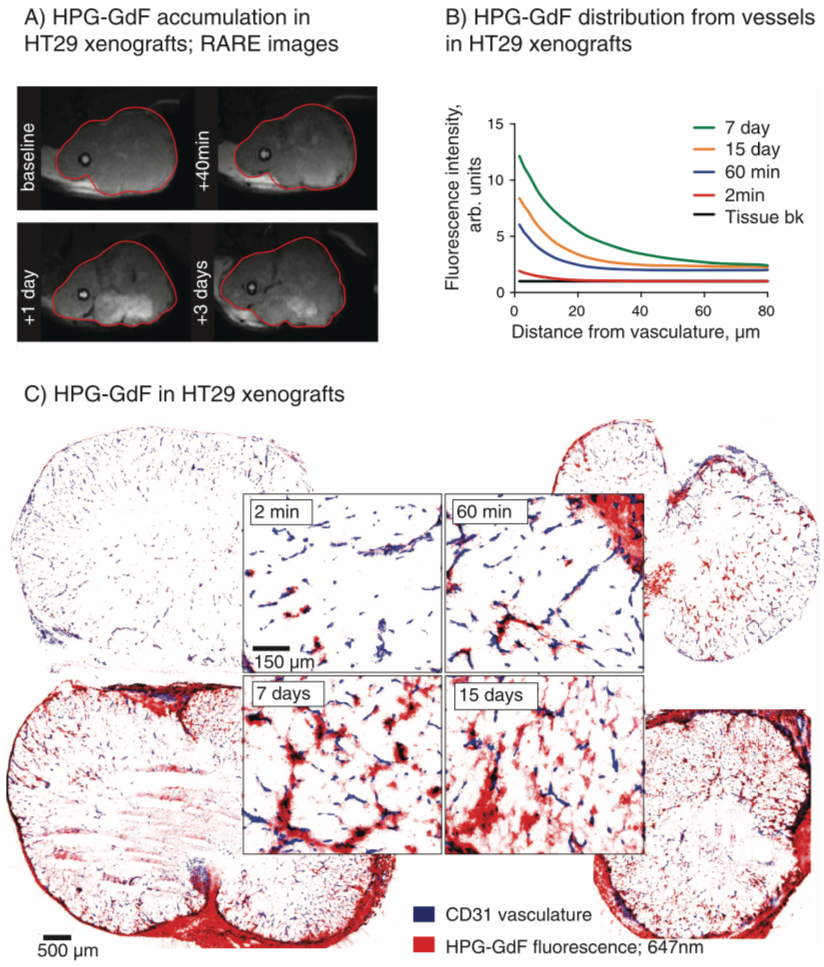
\includegraphics[width=\textwidth]{hpg/hpg-paper1-images/hpg_fig3-hpgdistribution.png}
 \caption{Accumulation and distribution of \acs{HPG-GdF} in HT29 xenografts. (A) T$_1$-weighted MR-RARE images show signal enhancement at 40 min that increases with longer exposures (HT29 tumours outlined in red). (B) Quantitative analysis of \acs{HPG-GdF} distribution relative to CD31-positive vessels shows extravasation of \acs{HPG-GdF} and distribution away from vessels to a limited distance, with a maximum at 7 days. (C) Whole tumour maps of \acs{HPG-GdF} (red) in relation to vasculature (blue) show that at early (2 min) timepoints \acs{HPG-GdF} is primarily overlapped with vasculature, but by 60 min there is substantial heterogeneity, where some vessels have greater amounts of perivascular \acs{HPG-GdF} than others. \acs{HPG-GdF} accumulates over several days but does so heterogeneously, and does not distribute through tumour tissue even after prolonged exposures.}
 \label{hpgpaper1:fig3}
 \end{center}
\end{figure}

\section{Results}

\subsection{HPG-GdF accumulates in tumour tissue in the extravascular space but does not distribute far from vasculature}

Averaged data from whole HT29 tumour xenograft images obtained using MRI and histology showed accumulation of \acs{HPG-GdF} over time (Fig.~\ref{hpgpaper1:fig3}(A)), as previously described~\cite{Saatchi:2012hc}.
HPG-GdF fluorescence was detectable within or very near to CD31-labeled tumour vessels as early as 2 min following contrast agent injection (Fig.~\ref{hpgpaper1:fig3}(B), (C)).
More HPGGdF fluorescence accumulated in histological tumour sections over time, but very little agent was observed at distances farther than 40 $\mu$m from the vasculature, even at 7 and 15 days (Fig.~\ref{hpgpaper1:fig3}(B), (C)).
By 60min there was extravascular accumulation of \acs{HPG-GdF} around some vessels, but considerable inter-vessel heterogeneity was observed.
Some vessels showed no \acs{HPG-GdF} fluorescence (Fig.~\ref{hpgpaper1:fig3}(C)).

\subsection{Bolus arrival time (BAT) for \acs{HPG-GdF} as a screen for viable tissue}

Maps of BAT overlaid on T$_1$-RARE images for both Gadovist and \acs{HPG-GdF} are shown in Fig.~\ref{hpgpaper1:fig4}, Rows 1 and 2.
A pattern of faster contrast enhancement at the tumour margins was consistent for both contrast agents.
While Gadovist eventually distributes to all the tissue, many voxels fail to enhance with \acs{HPG-GdF} within the 37 min imaging period.
Comparison of \acs{HPG-GdF} BAT-enhancing voxels with a histological image delineating viable versus necrotic tissue (Fig.~\ref{hpgpaper1:fig4}, Rows 2 and 3) shows that the non-enhancing voxels consistently corresponded to large areas of tumour necrosis.
A negative association was seen between the necrosis fraction determined by histology and the fraction of enhancing voxels for \acs{HPG-GdF} (Fig.~\ref{hpgpaper1:fig2}(C)).
For subsequent analysis of vascular function, only voxels enhancing with \acs{HPG-GdF} using the BAT criteria were evaluated.

\begin{figure}[htbp]
 \begin{center}
 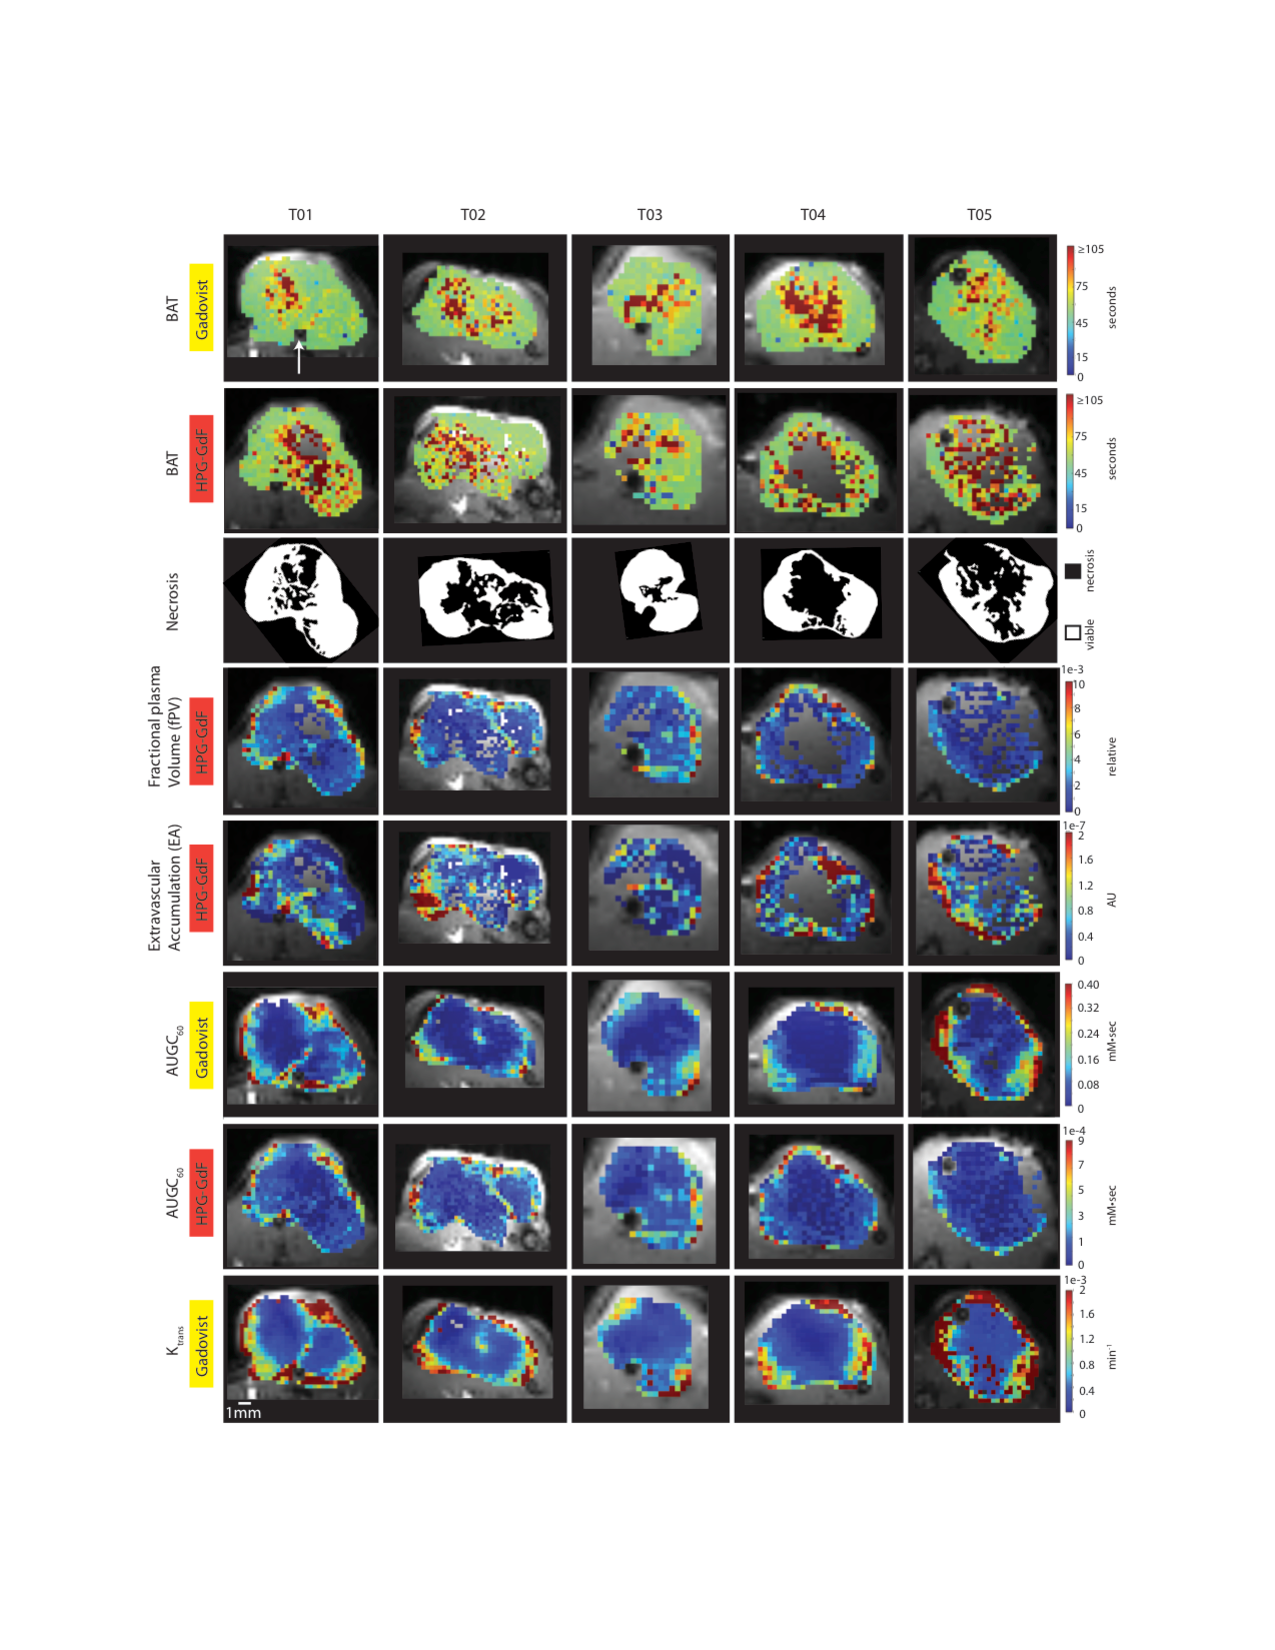
\includegraphics[width=0.8\textwidth]{hpg/hpg-paper1-images/hpg_fig4-ht29.pdf}
 \caption{Vascular function in HT29 xenografts. Whole-slice maps are presented for individual HT29 tumours (T01-T05, vertical columns) for parameters derived from MR imaging of Gadovist (BAT, AUGC60, K$^{trans}$), MR imaging of \acs{HPG-GdF} (BAT, fPv, \acs{aPS}, AUGC60) and histological imaging (necrosis). Good slice matching between imaging sessions is achieved using implanted fiducial marker tubes, an example of which is shown for tumour T01, Row 1, where the arrow points to the dark region where the tube is resting between the tumour and the back of the animal.}
 \label{hpgpaper1:fig4}
 \end{center}
\end{figure}

\subsection{Fractional plasma volume (fPV) and apparent permeability-surface area product (aPS) as measures of vascular function}

HPG-GdF-enhancing voxels were further characterized for their plasma volume (fPV) by calculating the magnitude of the rapid signal increase after injection and for their extravascular accumulation (apparent permeability-surface area product, \acs{aPS}) by measuring the slope of the enhancement curve after the initial increase for the duration of the DCE scan (0-2000 s).
The patterns of high and low \acs{fPV} and \acs{aPS} were often similar to each other, though there are notable differences.
A linear regression analysis comparing \acs{fPV} with \acs{aPS} for whole-slice averages yields an R$^2$ of 0.11, suggesting they are independent of each other.
As a detailed example, tumour HT01 has a region of high \acs{aPS} and low \acs{fPV} (Fig.~\ref{hpgpaper1:fig5}(A)), as well as a region exhibiting the opposite, with high \acs{fPV} and low \acs{aPS} (Fig.~\ref{hpgpaper1:fig5}(B)).
The corresponding histological section seemed to validate these observations, where the region with high \acs{fPV} has a greater density of CD31-stained vessels and the region with greater \acs{aPS} has more \acs{HPG-GdF} in the extravascular compartment.
While histological data enables a detailed view of \acs{HPG-GdF} accumulation, the actual rate of extravasation may only be determined by the dynamic MR data, as illustrated by the schematic enhancement curve (Fig.~\ref{hpgpaper1:fig5}(C)).
The corresponding K${trans}$ map derived from Gadovist concentrations shows high values in both the high \acs{aPS} and high \acs{fPV} regions of this tumour (Fig.~\ref{hpgpaper1:fig4}, Column 1).
Therefore, both \acs{fPV} and \acs{aPS} played important roles contributing to overall tumour vascular function, had measurable intra-tumour heterogeneity and produced data that was distinct from and more informative than DCE-MRI derived parameters for Gadovist.

\begin{figure}[htbp]
 \begin{center}
 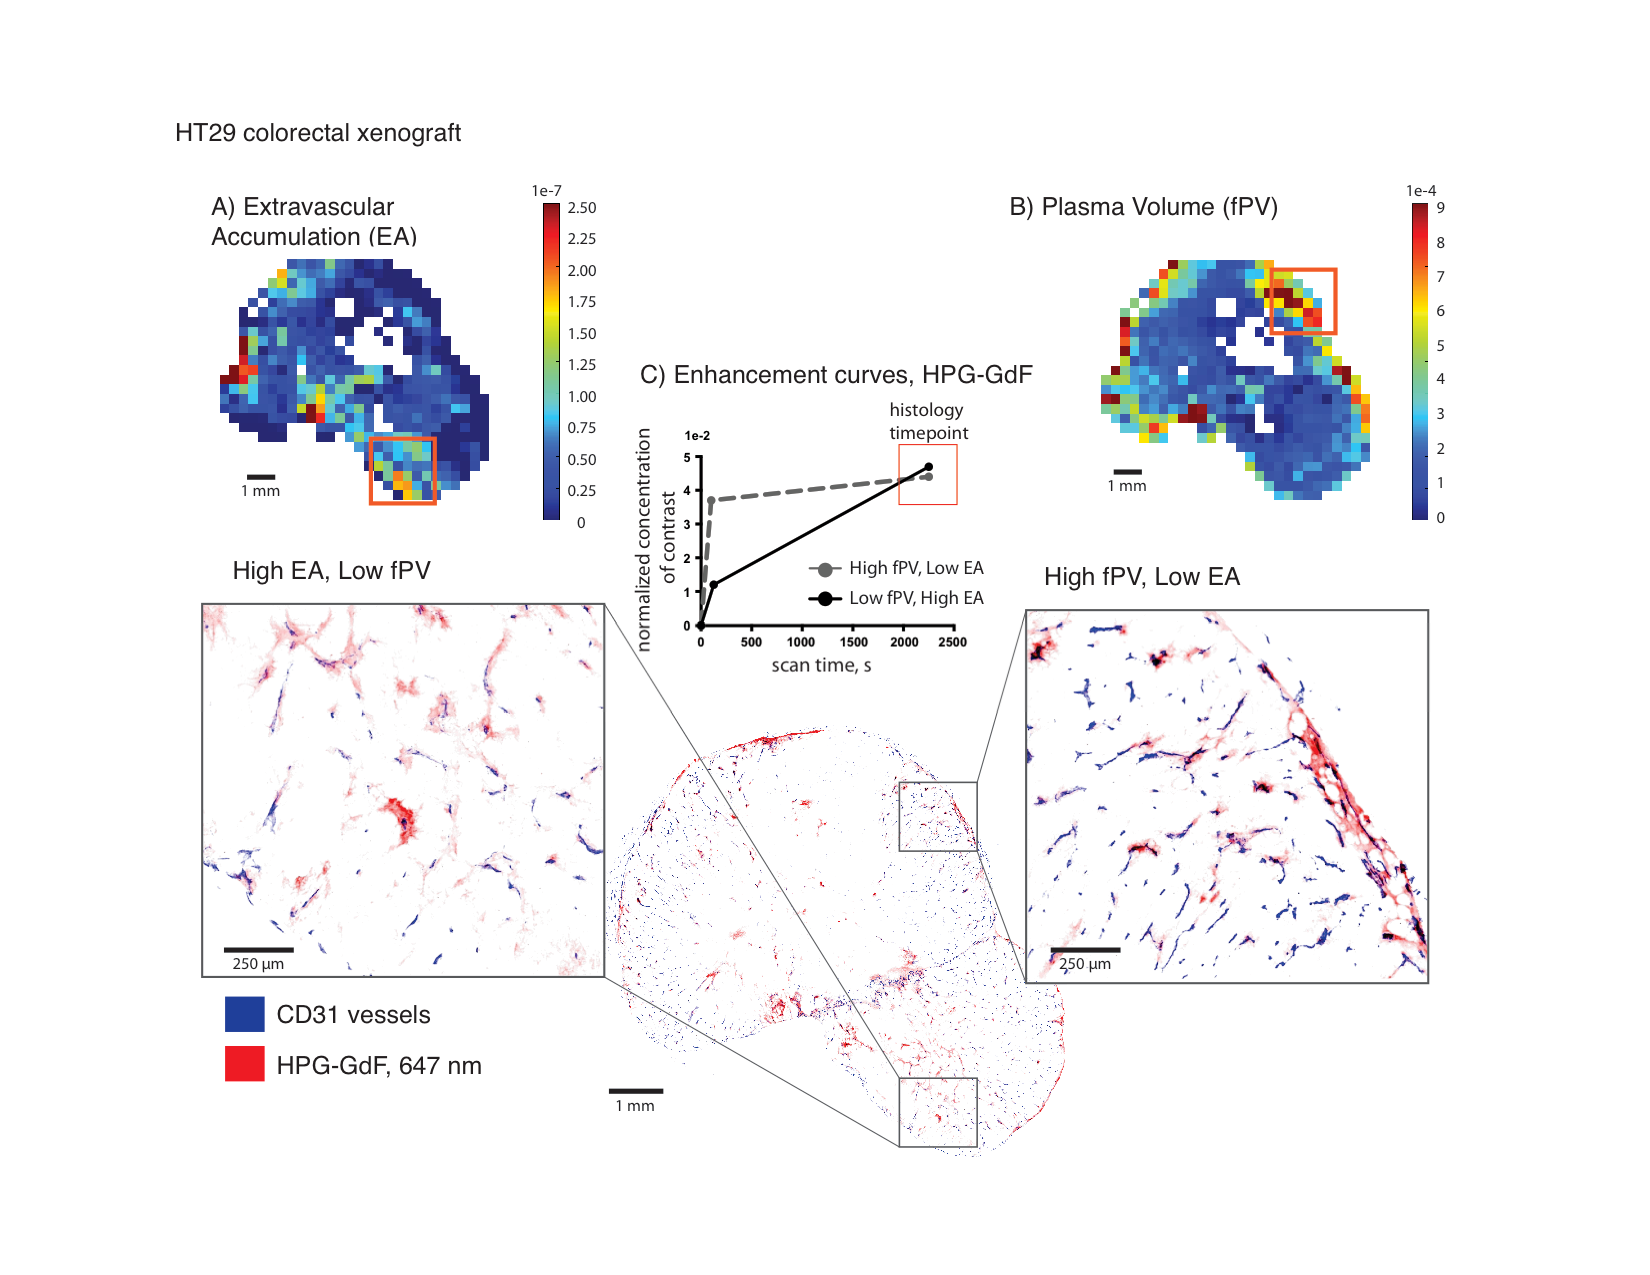
\includegraphics[width=\textwidth]{hpg/hpg-paper1-images/hpg_fig5-ht29fpv.pdf}
 \caption{fPv and \acs{aPS} in HT29 xenograft.
 Whole-slice parameter maps are presented for HT29 tumour (T01) with the corresponding histological image depicting CD31 stained vessels (blue) and \acs{HPG-GdF} native fluorescence (red).
 A region with high \acs{aPS} values that does not correspond to high \acs{fPV} is magnified (A) and compared with a region having high \acs{fPV} that does not correspond to high \acs{aPS} (B).
 The high \acs{fPV} region has notably greater vascular density, and \acs{HPG-GdF} is clearly seen overlapping with vessels (black) or accumulating in the extravascular space.
 The high \acs{aPS} region also has \acs{HPG-GdF} in the extravascular space.
 The dynamic MR-derived parameters are better able to illustrate the functional features of tumour vasculature than are the static histological data, which only reflects the environment at a single, terminal endpoint (C).}
 \label{hpgpaper1:fig5}
 \end{center}
\end{figure}

\begin{figure}[htbp]
 \begin{center}
 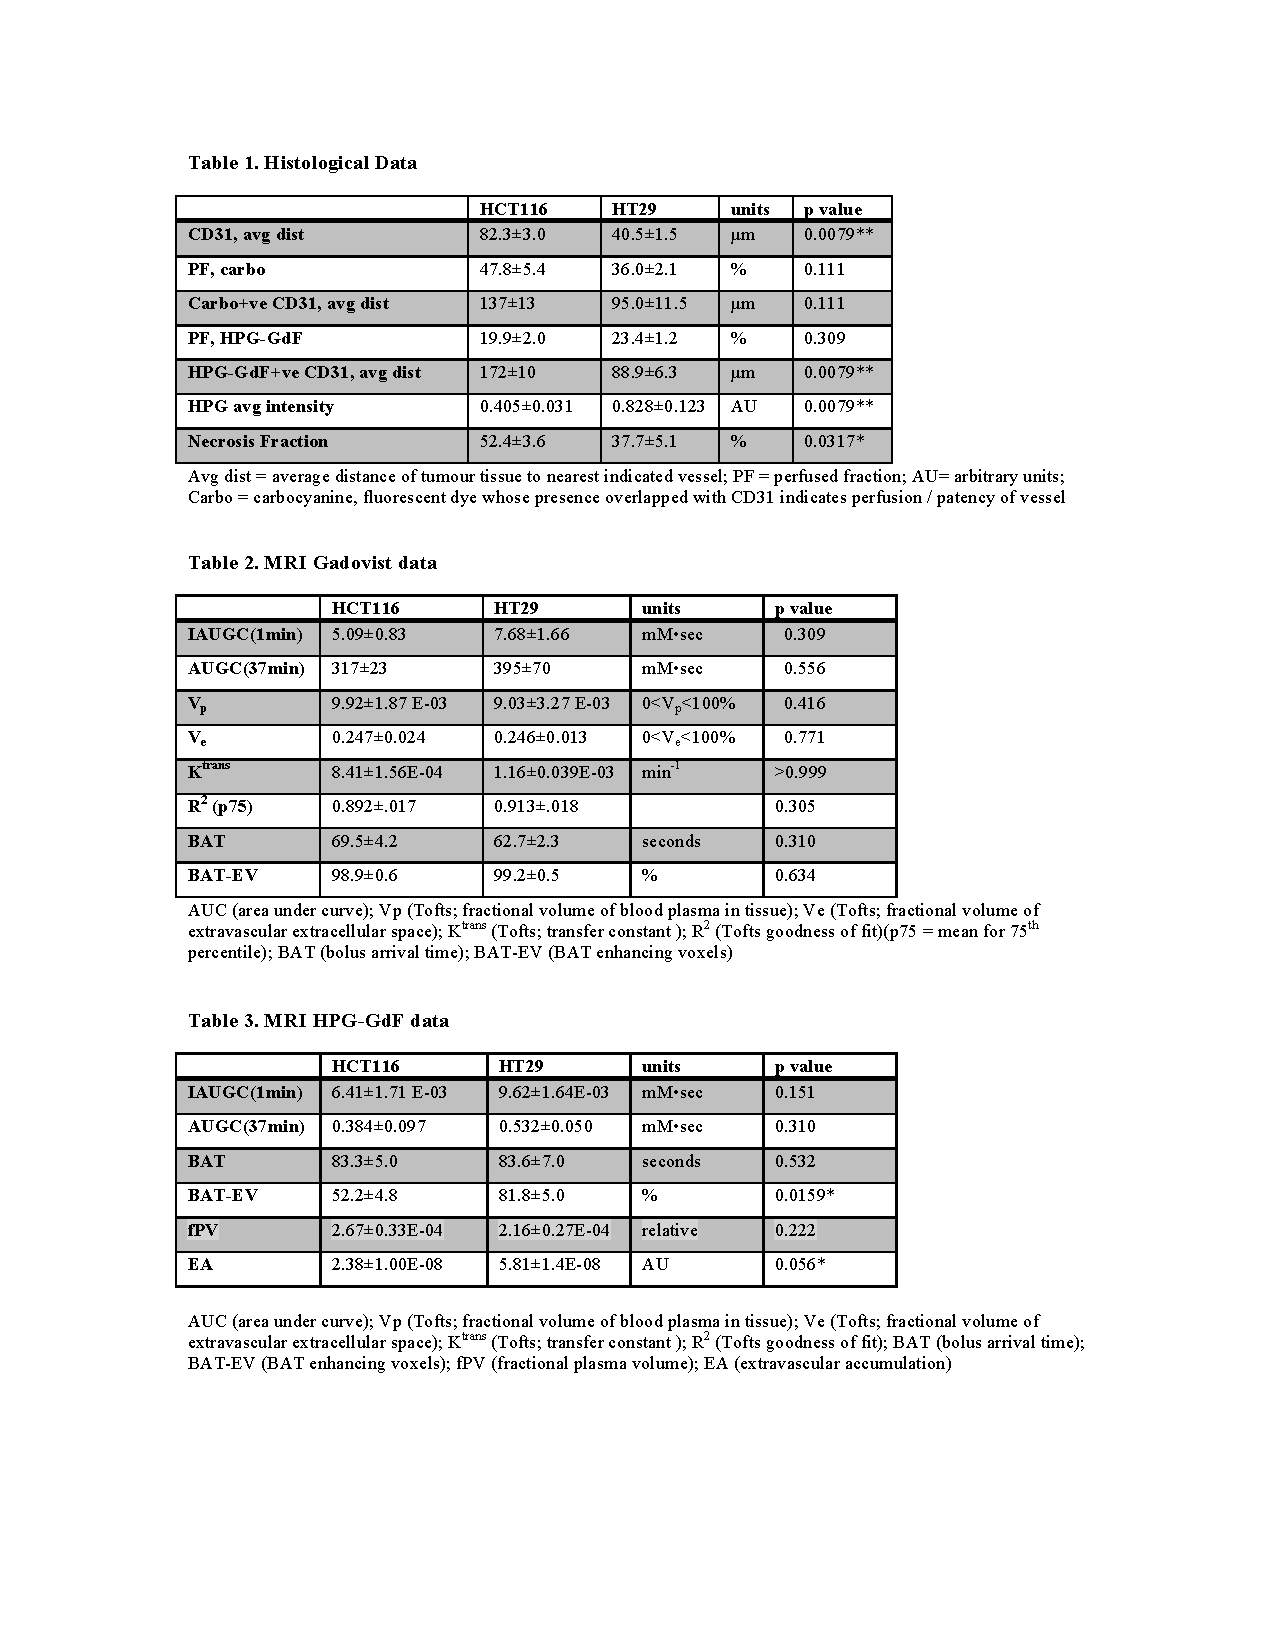
\includegraphics[width=\textwidth]{hpg/hpg-paper1-images/hpg_tables.pdf}
 \caption{ }
 \label{hpgpaper1:tables}
 \end{center}
\end{figure}

\subsection{Variable vascular function in HCT116 and HT29 human colorectal xenografts}

HPG-GdF accumulated to a greater degree in HT29 colorectal xenografts relative to HCT116, and this was seen at all distances from vessels (Fig.~\ref{hpgpaper1:fig6}(A)).
HCT116 and HT29 colorectal xenografts grow at similar rates in mouse models but exhibit distinct vascular function parameters (data summarized in Table 1).
Overall, HT29 tumours possessed a greater density of vessels (CD31 average distance was 82.3 $\pm$ 3.0 $\mu$m for HCT116 and 40.5 $\pm$ 1.5 $\mu$m for HT29, p < 0.05*).
However many vessels were unlabeled for the fluorescent dye (carbocyanine) used as a histological perfusion marker; the density of perfused vessels was similar between the two xenograft models (CD31 vessels labeled for carbocyanine, PF, was 47.8$\pm$5.4\% for HCT116 and 36.0$\pm$2.1\% for HT29, p > 0.05).
The density of vessels labeled for HPG-GdF fluorescence was much greater in HT29 tumours (HPG-GdF+ve CD31, average distance was 172$\pm$10$\mu$m for HCT116 and 88.9 $\pm$6.3$\mu$m; p<0.05*).
In addition to a greater density of HPGGdF-positive vessels, the high MW contrast agent was able to accumulate to a greater degree in the extravascular space around vessels in HT29 cells.
This effect can be seen in the histological images of the compared tumour models collected 60min post HPG-GdF administration (Fig.~\ref{hpgpaper1:fig6}(B)).

\subsection{MRI analysis of HPG-GdF in HCT116 and HT29 xenografts: BAT, fPV and aPS}

Administration of neither Gadovist nor HPG-GdF was useful in detecting the difference in vascular function between HCT116 and HT29 tumours using the initial area under the gadolinium concentration curve (AUGC), as the slice-averaged means were not significantly different between tumour groups (AUGC for Gadovist in HCT116 was 5.09 $\pm$ 0.83 mM s and that in HT29 was 7.68 $\pm$ 1.66 mM s, p > 0.05; that for HPG-GdF in HCT116 was 6.41 $\pm$1.71x10$^{-1}$3 mMs and that in HT29 was 9.62$\pm$1.64x10$^{-1}$3 mMs, p > 0.05) (data summarized in Tables 2 and 3).
Similarity between models was also observed qualitatively in the parameter maps with AUGC or K${trans}$ overlaid on T$_1$-RARE images shown in Figs.
4 and 7.
Both tumour models show higher AUGC values in the tumour margins for both contrast agents.

\begin{figure}[htbp]
 \begin{center}
 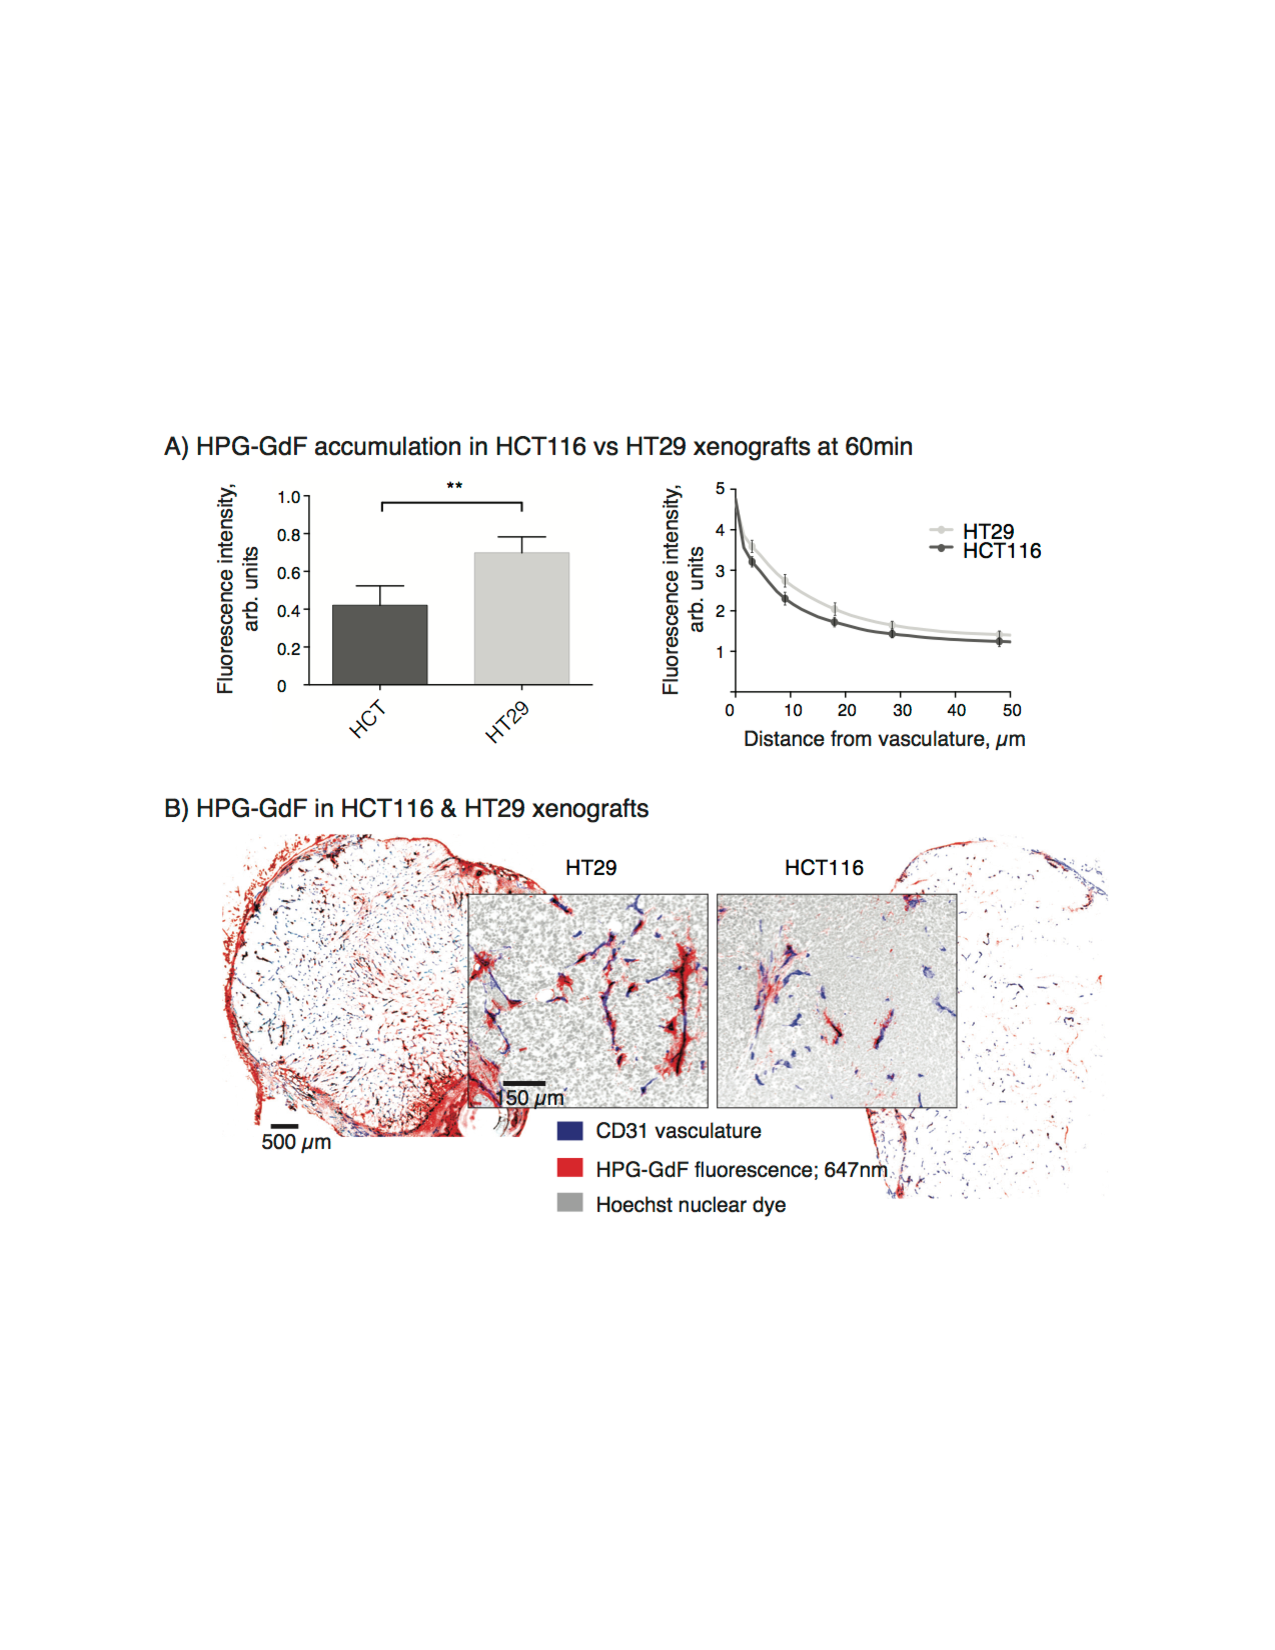
\includegraphics[width=\textwidth]{hpg/hpg-paper1-images/hpg_fig6-accumulation.pdf}
 \caption{HPG-GdF distribution in HCT116 and HT29 colorectal tumour xenografts at 60 min: histological analysis.
 (A) The whole-slice average fluorescence intensity shows that HPG-GdF accumulates to a greater degree and distributes further away from vasculature in HT29 tumours.
 (B) Sample images show HPG-GdF (red) overlaid on CD31 (blue); insets also display nuclear density (grey).
 A greater degree of HPG-GdF accumulation can easily be appreciated in the HT29 tumours.}
 \label{hpgpaper1:fig6}
 \end{center}
\end{figure}

However, an MR-measured difference between HCT116 and HT29 vascular function was seen with the BAT data for HPGGdF, as the fraction of enhancing voxels was significantly lower in the HCT116 relative to the HT29 tumours (BAT-EV for HPGGdF in HCT116 was 52.2 $\pm$ 4.8\% and that in HT29 was 81.8 $\pm$ 5.0\%, p < 0.05*) (Table 3).
This corresponded to the histological data, which also shows HCT116 tumours as having a greater proportion of necrotic tissue (necrosis fraction for HCT116 was 52.4$\pm$3.6\% versus 37.7$\pm$5.1\% in HT29, p<0.05*).
Of the HPGGdF BAT-enhancing voxels, the averaged fPV and aPS parameters were also determined (Table 3), and no difference was seen with the plasma volume between tumour models (fractional fPV for HCT116 is 2.67 $\pm$ 0.33 x 10$^{-1}$4 and that for HT29 is 2.16 $\pm$ 0.27 x 10$^{-1}$4, p > 0.05), but a trend of greater aPS was seen in the HT29 xenografts (aPS for HCT116 was 2.38 $\pm$ 1.00 x 10$^{-1}$8 and that for HT29 was 5.81 $\pm$ 1.4 x 10$^{-1}$8, p = 0.056*).
aPS of HPGGdF was the only MR-derived biomarker able to detect the significant difference in vascular function between these two tumour models.
Complete data sets for HCT116 tumours are shown in Fig.~\ref{hpgpaper1:fig7}.

\section{Discussion}

The use of MCAs for imaging and describing tumour vascular function is a widely pursued area of research.
Many studies have investigated a range of sizes, where smaller molecules extravasate and distribute through tissue too quickly to be considered as sensitive blood pool agents, and larger molecules often accumulate too slowly for adequate signal detection~\cite{Kyle:2007ch,Tang:2013fi,Sourbron:2011ce}.
In this work we describe HPG-GdF as an MR-visible MCA of 583 kDa, for which we have derived useful biomarkers that have sensitivity in measuring vascular function.
While the signal-to-noise from HPG-GdF concentration-time curves is not adequate to fit a complex pharmacokinetic model to determine parameters such as v$_p$, v$_e$ and K$^{trans}$, enhancement was measurable in most tumour voxels.
The number of Gd chelates on the HPG-GdF is approximately 300 per carrier molecule, which is high relative to many albumin chelates, the most common MCA in preclinical use, which typically have about 20 chelates per carrier~\cite{Ogan:1987tg}.
In addition to a greater number of Gd per carrier, the HPG-GdF accumulates in the perivascular space and fails to distribute more than a few micrometers from most vessels within a short DCE imaging timeframe (Fig.~\ref{hpgpaper1:fig3}).
This accumulation could provide a greater concentration for detection of a local, permeable tumour vessel and avoids the risk of conflating this with the distribution and accumulation elsewhere in tumours.
These attributes of HPG-GdF may make it more sensitive and more specific than a smaller MCA such as albumin-Gd-DTPA.
A minimum DCE imaging time from the presented data would appear to be about 15 min for the analyses described, which is longer than the suggested 5min ideal for practical clinical utility~\cite{Turetschek:2004bw}.
It is possible that greater signal could also be obtained by decreasing the time resolution from the 2.4s used in these studies, since HPG-GdF remains largely intravascular.
HPG-GdF contains the Gd-DOTA complex, which is highly thermodynamically stable and kinetically inert.
The dissociation constant for Gd-DOTA (log K = 24.7) is much higher than those for CaDOTA (log K = 17.23) or Mg-DOTA (log K = 11.92), hence neither Ca nor Mg can transmetallate Gd from the Gd-DOTA complex~\cite{Baranyai:2005ta}.
Biodegradation of HPG-GdF is therefore likely minimal, occurring through enzymatic attack of the end group, similar to that seen for polyethylene glycol~\cite{Kawai:2002fc}.
However, the long half-life and relatively slow excretion of HPGs through the reticuloendothelial system of the liver suggest that the potential for toxicity should be investigated and monitored.
A biodegradable version of HPG has recently been synthesized and might circumvent these potential concerns, and will be a focus in future DCE studies investigating the use of HPGs as MR-visible MCAs~\cite{Shenoi:2013id}.
Limited extravasation of HPG-GdF is likely due to the selective permeability of tumour vessels with adequate pore sizes for passage of the bulky molecule, a phenomenon described as the enhanced permeability and retention (EPR) effect~\cite{Maeda:2013hq}.
Limited distribution through the interstitium is also most probably the result of its significant size.
We have observed HPG-GdF to be much more restricted in its distribution than is suggested by the diffusion coefficients (D(HPG) = 3.7 x 10$^{-1}$7 cm$^2$ s$^{-1}$1 and D(Gadovist) = 3.6 x 10$^{-1}$6 cm$^2$ s$^{-1}$1), as the larger agent reaches only 10-15$\mu$m away from vessels within an hour whereas Gadovist reaches all areas of a tumour.
HPG-GdF molecules experience greater obstacles to their movement through the heterogeneous tumour microenvironment due to their size, but also possibly due to steric hindrances, non-specific binding or sequestration~\cite{Minchinton:2006gs}.
The large size of HPG-GdF is a significant advantage.
An approximately exponential increase in sensitivity for detection of permeability has been reported with increasing MCA size (19).
If extravasation of HPG-GdF only occurs in vessels that are permeable, and the agent does not distribute through the extravascular space to distances away from vessels, then MR-visible HPG-GdF enhancement suggests the presence of vasculature, and accumulation of the agent over time indicates the local presence of a hyperpermeable vessel.

\begin{figure}[htbp]
 \begin{center}
 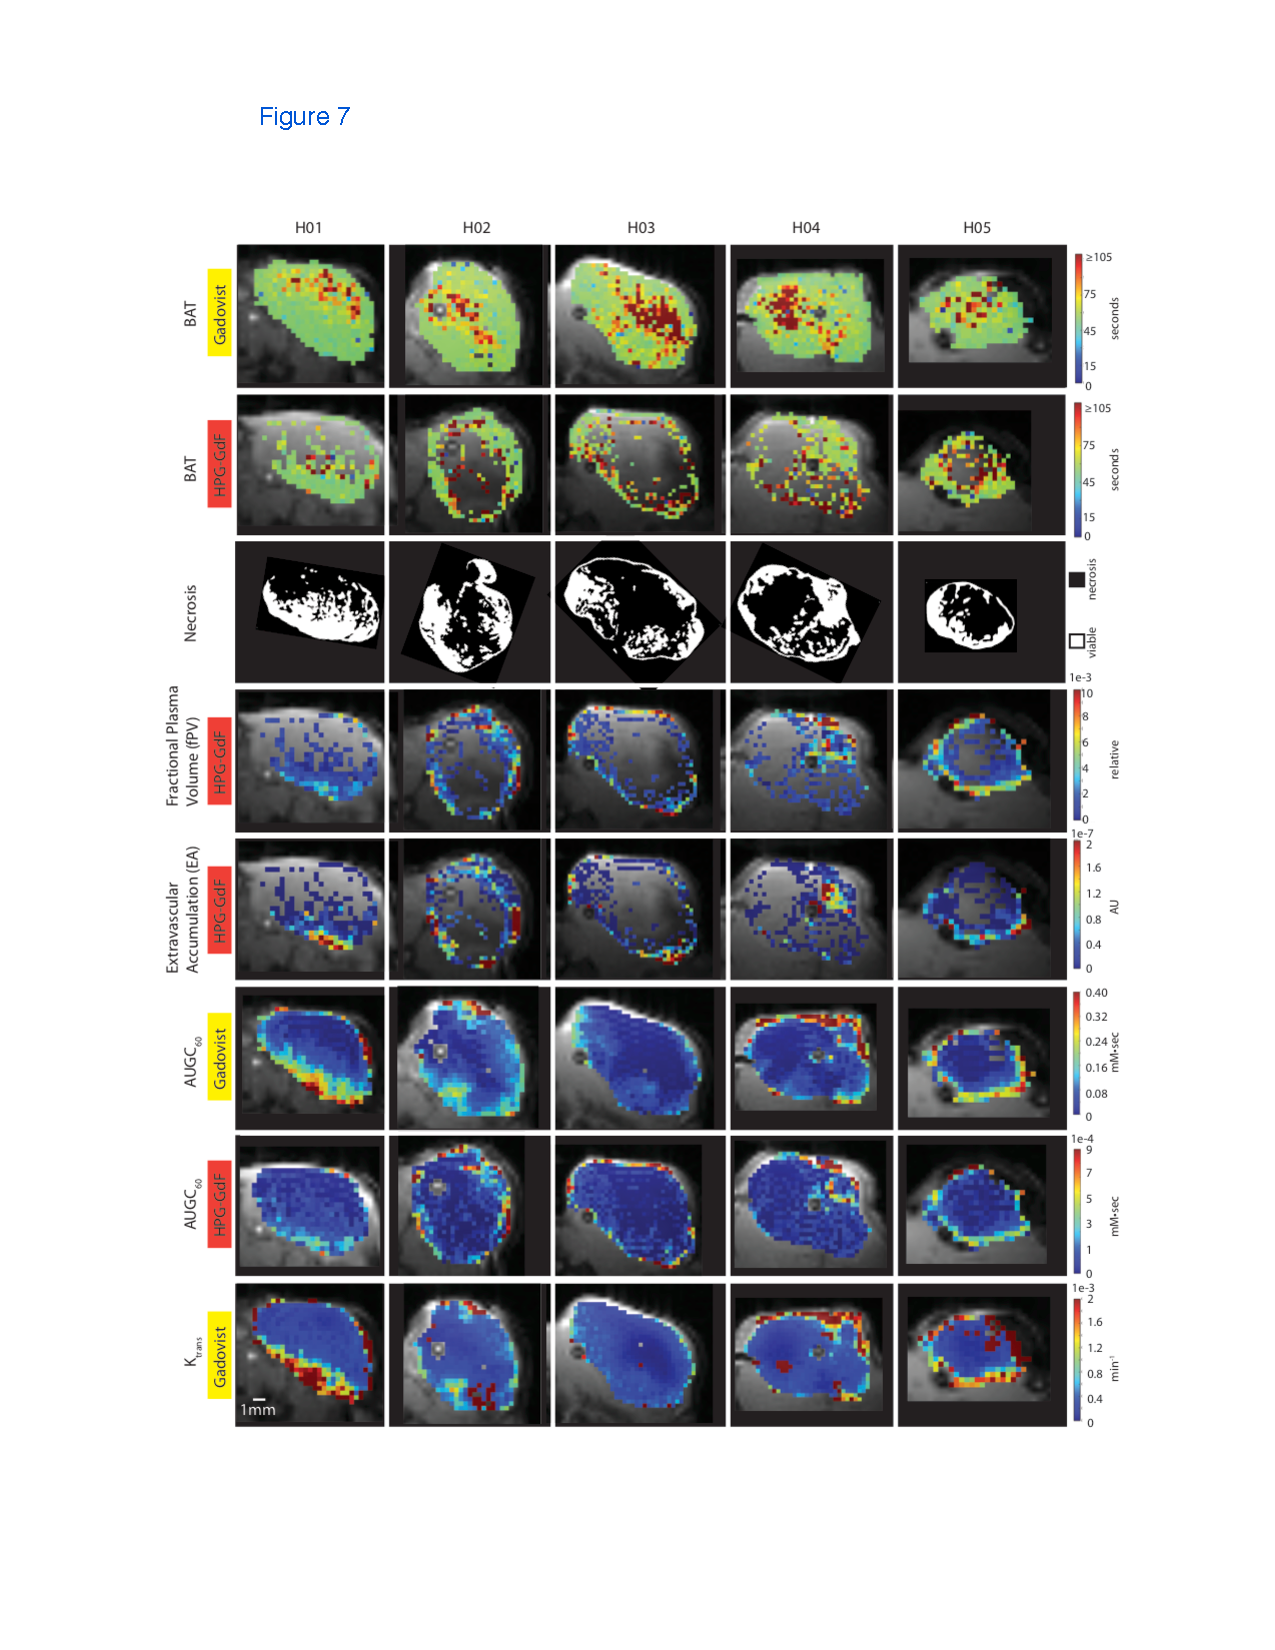
\includegraphics[width=0.8\textwidth]{hpg/hpg-paper1-images/hpg_fig7-hct116.pdf}
 \caption{Vascular function in HCT116 xenografts. Whole-slice maps are presented for individual HCT116 tumours (T01-T05, vertical columns) for parameters derived from MR imaging of Gadovist (BAT, AUGC60, K$^{trans}$), MR imaging of HPG-GdF (BAT, fPv, aPS, AUGC60) and histological imaging (necrosis).}
 \label{hpgpaper1:fig7}
 \end{center}
\end{figure}

A typical enhancement curve for HPG-GdF is shown in Fig.~\ref{hpgpaper1:fig2}.
The size of the initial step-like enhancement is interpreted as the fPV, and the slope of signal change for the remaining enhancement is reported as the aPS, reflecting the extravascular accumulation of HPG-GdF (Fig.~\ref{hpgpaper1:fig2}).
These parameters are not correlated with each other, with either value potentially significantly higher or lower than the other in the same voxels (Fig.~\ref{hpgpaper1:fig5}).
A pattern of faster enhancement at the tumour margins is consistent for both contrast agents, and, while Gadovist eventually arrives in all the tissue, including regions of necrosis, many voxels that correspond to necrotic regions fail to enhance with HPG-GdF within the 37 min imaging session.
We found that HPG-GdF BAT-enhancing voxels correspond to areas without necrosis: see Figs.~\ref{hpgpaper1:fig4} and ~\ref{hpgpaper1:fig7} for parameter maps of all BAT-enhancing voxels compared with histologically validated necrotic regions.
Therefore, we identified perfused regions of tumour tissue for further vascular function analysis using the straightforward approach of selecting voxels that had positive BATs for their HPG-GdF enhancement curves.
Selection of viable tissue and the exclusion of necrotic tissue is a desirable approach for controlling for inter-tumour heterogeneity, since MRI data is most often described as a whole-tumour average.
In the event that different tumours possess variable necrotic burdens, or if the necrotic fraction increases over time with treatment, selective analysis of viable tissue can control for this variability.
Qualitative comparisons of well-matched, whole-slice images from multiple modalities emphasize the utility of screening for BAT-enhancing voxels to select for perfused and viable tissues.

Without this information analysis may be restricted to regions of tissues at the tumour margins where hot spots of vascularization are observed histologically, and tissue is assumed to be viable in the MR image~\cite{Pathak:2005gu,Li:2005gw}.
In the colorectal xenografts examined here the amount of necrosis varied considerably, and, while it is typically located more in the core than the tumour margins, there is substantial inter-tumour heterogeneity with respect to the amount and location of necrosis.
Notably, while the values for K$^{trans}$(Gadovist) are on average higher around the entire tumour rim, the fPV and aPS values are more heterogeneously arranged around the rim and within the interior of the tumour.
Our more comprehensive approach, validated by observations of viable tissue and perfused vessels within tumour interiors in histological sections, is a significant improvement over selectively assessing limited regions or hotspots for histological or MR quantitative analysis.
Traditional DCE-derived parameters such as AUC and K$^{trans}$ are composite measures influenced to varying degrees by vascular surface area, permeability and blood flow.
Our histological data supports a significant range in the propensity for HPG-GdF to extravasate, suggesting that assumptions of perfusion or permeability-limited conditions are not applicable to all areas of the tumour microenvironment.
Hence, we cannot conclude that aPS is exclusively proportional to permeability-surface area (PS) in the whole microenvironment.
For example, although the amount of HPG-GdF leaking into the extravascular space is dependent on the vessel being permeable to large molecules, the amount of accumulation, and therefore the amount of signal enhancement, may still be impacted by the concentration of contrast agent within the vessel.
Longitudinal gradients can occur locally in permeable vessels as the contrast agent leaks out, despite plasma concentrations remaining consistent in overall systemic circulation~\cite{Erickson:2003wt,Dewhirst:1999jh}.
Thus, the aPS is a measure of vascular function that has contributions from permeability as well as, when permeability is very high, perfusion.
These limitations in the physiological interpretation of aPS are similar to those that apply to K$_{trans}$ and AUC for all contrast-enhanced modelling.
Parameters that are based on the amount and proportion of contrast agent enhancement are dependent on fewer assumptions than are pharmacokinetic model-derived parameters such as K$^{trans}$.
Biophysical signals are dependent on the many variables necessarily involved in obtaining MR images, such as the scanner, imaging sequence, RF coil and analysis techniques.
Interpreting magnitudes of change in highly variable tumours may be more reliable than assuming invariable pharmacokinetic attributes or unchanging tumour microenvironments, and may make simplified biomarkers such as fPV and aPS more applicable to clinical studies conducted across multiple centres~\cite{OConnor:2012ie}

\section{Conclusion}

HPG-GdF is a largely intravascular MCA that selectively extravasates from hyperpermeable tumour vessels, accumulating in the perivascular regions without distributing through the tumour interstitium.
The high concentration of Gd chelates per carrier molecule in combination with its excellent solubility makes HPG-GdF detection possible despite the relatively low plasma fraction within tumours.
By carefully comparing the vessel parameters of small and large molecule contrast agents in the same tumour, as well as comprehensively assessing the location of MCA within the tumour relative to vasculature and necrosis, we conclude that BAT, fPV and aPS biomarkers derived from HPG-GdF enhancement provide a sensitive and specific approach to measuring tumour vascular function.
HPG-GdF and these analysis techniques would be appropriate in the evaluation of tumour angiogenesis and response to treatment for preclinical research, with potential for eventual translation to the clinic.


\endinput

%% The following is a directive for TeXShop to indicate the main file
%%!TEX root = ../diss.tex

\chapter{Using \acs{HPG-GdF} to investigate distribution of trastuzumab.}
\label{ch:HPG2}

%\section{Preface}
%\SARi{There is no preface in the previous chapter - why here not there? Does it need a special heading?}
%In this chapter, we describe an application of the novel contrast agent \acs{HPG-GdF} in pre-clinical animal research on chemotherapies.
%The sections reproduced here in this chapter were part of a larger study exploring the distribution of trastuzumab, including exploring the microenvironments of \acs{HER2}-positive tumours and metastases including immunohistochemistry maps, 3D tissue models and dynamic imaging of tumour vasculature.
%This work was led by Dr.\ Jennifer Baker and the Andrew Minchinton lab in collaboration with the Reinsberg lab and published, with me as the fourth author in the peer-reviewed journal \emph{Clinical \& Experimental Metastasis} \deleted{with the manuscript} titled ``Heterogeneous distribution of trastuzumab in \acs{HER2}-positive xenografts and metastases: role of the tumor microenvironment''.

\section{Introduction}

Treatment options for patients with the aggressive \acs{HER2}-positive form of breast cancer continue to improve, though metastatic breast cancer remains a largely incurable disease.
Brain metastases are of particular importance in \acs{HER2}-positive breast cancer patients.
With improved treatments and prolonged survival, the incidence of brain metastases as the first evidence of relapse has increased~\cite{Seal:2012cn,Bria:2007gc}.
This effect has been attributed to the the blood-brain barrier (\acs{BBB}) creating a sanctuary site by preventing drug access~\cite{Kaplan:2014es,Lai:2004bd}.
Antibody-based therapeutics such as trastuzumab are proposed to have difficulty crossing the \acs{BBB} and therefore brain metastases evade drug activity~\cite{Seal:2012cn,Murrell:2015bz,Stemmler:2006}.
In addition to the \acs{BBB}, specific characteristics of the tumour microenvironment, beginning with a relative paucity of functional vessels, can thwart the access of drugs to their targets such that a population of under-exposed cells may survive and repopulate the tumour~\cite{Minchinton:2006gs}.
We have demonstrated that many small molecule cytotoxics have limited tumour tissue penetration in both in\replaced{-vitro}{ vivo} and in\added{-}vivo model systems due to difficulties with drug supply, flux through tissue, consumption or sequestration by cancer cells close to blood vessels~\cite{Kyle:2014cy,Kyle:2007ch,Huxham:2004hm,Kyle:2004fo,Kyle:1999kr}.

Macromolecular compounds such as \acs{MAb} face particular extravascular distribution difficulties due to their high molecular weights and target-binding affinity~\cite{Jain:2010ie,Chauhan:2011fi}.
The relatively slow distribution of \acs{MAb}s has been attributed to the binding site barrier hypothesis, where in the case of high affinity binding of the \acs{MAb} to antigen, \acs{MAb} distribution is limited by its binding in the presence of ample antigen~\cite{Juweid:1992ty}.
Data from our collaborators' lab (Dr. Andrew Minchinton) in the vector over-expressed MDA-435-LCC6 \acs{HER2} model showed that despite the ability of trastuzumab to distribute far from vessels in tumours with relatively even \acs{HER2} distribution, there persisted \acs{HER2}-positive tissue with poor access to trastuzumab after peak plasma exposures~\cite{Baker:2008ci}.
Staining heterogeneity is very striking at the vessel level, as trastuzumab is able to extravasate from only a subpopulation of perfused vessels.
\todo[backgroundcolor=blue!20!white]{is the limitation focusing on net tumour accumulation or the hetrogeneity or smth else?}
Other groups have also demonstrated a limitation on the accumulation of trastuzumab in tumours, focusing on net tumour accumulation~\cite{Jain:2010ie,Chauhan:2011fi,Lee:2010gb}.

The ability of a drug to access and affect all its target cells is intuitively crucial for treatment success.
The relatively slow distribution of \acs{MAb}s through the interstitium in solid tumours is recognized, but the long half-life of \acs{MAb}s and prolonged plasma exposure is expected to ensure adequate time to access all the tissues in most treatment scenarios.
However, we have found that in addition to distributing slowly, \acs{MAb}s experience additional barriers, leaving some areas of tissue with inadequate drug exposure.
The aim for this study was to use \acs{HER2}-positive tumour and metastases models of cancer to determine potential limits to trastuzumab access that may represent a mechanism of resistance to targeted therapies.
%The microenvironments of \acs{HER2}-positive tumours and metastases are examined in detail using immunohistochemistry maps, 3D tissue models and dynamic imaging of tumour vasculature.

\section{Methods}

\subsection{Reagents}

trastuzumab and bevacizumab (Roche, Genentech) were provided by the British Columbia Cancer Agency pharmacy; dilutions to 1-2 mg/ml were prepared in sterile 0.9\% NaCl before intra-peritoneal (\acs{i.p.}) injection.
%Human isotype control IgG1 (Sigma) was administered from similar concentrations.
trastuzumab antibodies for use in combination with bevacizumab were tagged with fluorescent labels according to Alexa Fluor 546 Protein Labeling Kit (ThermoFisher) instructions.
%trastuzumab and IgG antibodies for use in combination with bevacizumab were tagged with fluorescent labels according to Alexa Fluor 546 Protein Labeling Kit (ThermoFisher) instructions.
Hypoxia marker pimonidazole (Hypoxyprobe) was administered at 60 mg/kg as an \acs{i.p.} injection 2 h prior to tissue harvest.
Fluorescent dye DiOC7(3) (Molecular Probes), 0.6 mg/ml dissolved in 75\% (v/v) dimethyl sulfoxide/25\% sterile H2O, was administered intravenously as a marker of vessel perfusion 5-min prior to tissue harvest~\cite{Trotter:1989cs}.

\subsection{Mice and tumours}

Female NOD-SCID mice weighing 20-28 g between 8 and 16 weeks of age were bred and maintained in our institutional pathogen free animal facility.
Mice were implanted with 60 day 17-$\beta$-estradiol pellets (Innovative Research of America) subcutaneously 3 days before implantation of \acs{BT474} or \acs{MDA-MB-361} tumours.
Tumors were implanted as single cell suspensions (2-10$\times 10^6$ cells) into the subcutaneous sacral region or into the inguinal mammary fat pads.
Metastases models were implanted as single cell suspensions (2-5$\times 10^5$ cells per implant) as \acs{i.v.} or \acs{i.p.} injections for SKOV3 or \acs{BT474} models, or as intra-cardiac injection for MDA-MDA-MB-231-BR-\acs{HER2} models, with animals euthanized a maximum of 23 days after implant.

\subsection{MRI}
MRI experiments were performed at the UBC MRI Research Centre on a 7T Bruker Biospec 70/30 scanner at room temperature with a combination volume (transmit)/surface (receive) coil.
\acs{DCE-MRI} data was collected as previously described~\cite{Baker:2015cob}.
Gadovist (Bayer Healthcare) was administered by \acs{i.v.} catheter as a 5 $\mu$L/g bolus dose from 60 mM solution.
Macromolecular contrast agent hyperbranched polyglycerol (\acs{HPG-GdF}, 583 kDa) was synthesized as previously described~\cite{Kainthan:2006ce,Saatchi:2012hc} and administered as a 6 $\mu$L/g bolus dose from 100 mg/mL (0.2 mM).
Regions of interest (ROI) were drawn on T$_2$-weighted \acs{RARE} images to outline the tumour using ImageJ (NIH) and all other MR analysis was performed using Python.
Area Under the Curves (AUC) for Gadovist was determined from the common injection time point to 60 s.
A two-parameter linear model was applied to characterize \acs{HPG-GdF} signal-intensity curves for fractional plasma volume (fPV) determined by the rapid increase at time of injection and for apparent permeability surface area product (aPS) calculated as the slope of later enhancement, as described earlier in section~\ref{hpgpaper1_methods}.
Both MR and histological modalities imaged slices in the plane perpendicular to an implanted fiducial marker tube to minimize angular differences between MR and histological image slices~\cite{Bains:2009hh}.

\subsection{Immunohistochemistry}
The general immunohistochemical procedure used has been previously reported~\cite{Baker:2008ci}.
Briefly, 10 $\mu$m tumour cryosections were air-dried, imaged for native DiOC7(3) or Alexa 546-tagged trastuzumab fluorescence, and fixed in 50\% (v/v) acetone/methanol for 10-min at room temperature.
trastuzumab was visualized in sections using Alexa 546 goat anti-human secondary antibody (Invitrogen)
%trastuzumab and IgG were visualized in sections using Alexa 546 goat anti-human secondary antibody (Invitrogen).
\acs{HER2} was subsequently stained with 2.2$\times 10^{-3}$ mg/mL trastuzumab as a primary detection antibody and goat anti-human Alexa 546 secondary.
Additional staining was performed using antibodies to PECAM/CD31 (BD PharMingen), pimonidazole (hypoxprobe) collagen IV (Gene Tex) and $\alpha$SMA (Abcam).
Visualization of primary detection antibodies was done using Alexa fluorescence secondary antibodies of appropriate species using 488 nm, 647 nm and 750 nm wavelengths.
Nuclear density was stained using Hoechst 33342 (Thermofisher) and imaged at 380 nm.

\subsection{Image acquisition and analysis}
Sections were imaged as previously described~\cite{Kyle:2007ch} using a system of tiling adjacent microscope fields of view at a resolution of 0.75 $\mu$m/pixel.
Using ImageJ~\cite{Collins:2007jr} and user-supplied algorithms, images were superimposed and manually cropped to tumour tissue boundaries with staining artifacts and necrosis removed.
False color images were constructed in ImageJ by converting greyscale images to color and overlaying selected layers: trastuzumab (magenta), \acs{HER2} (blue or grey), Hoechst 33342 (grey), CD31 (blue), carbocyanine (cyan), pimonidazole (green) and $\alpha$SMA or CIV (red).
Positive fluorescent staining is reported as average intensity (range 1-255) for pimonidazole, trastuzumab and \acs{HER2}.
Perfused vascular density was determined by applying a threshold to CD31 and DiOC7(3) images, with neighboring positive pixels grouped as ``objects''; CD31 objects with a minimum 20\% overlap with DiOC7(3) objects were determined to be perfused vessels.
All image pixels were sorted based on their nearest perfused vessel and the average distance is reported as a repeatable measure of vascular density.

\section{Results}

\subsection{Measures of vascular density, architecture and function do not consistently correlate with heterogeneous patterns of trastuzumab distribution}

Significant inter-vessel heterogeneity in trastuzumab distribution is seen in orthotopic \acs{BT474} xenografts, with neighbouring patent vessels often showing variable amounts of trastuzumab bound to perivascular cells (Fig.~\ref{hpgpaper2:fig4}A), similar to previous findings in MDA-435-LCC6 vector-overexpressing \acs{HER2}-positive tumours~\cite{Baker:2008ci}.
Non-patent vessels (purple arrows in Fig.~\ref{hpgpaper2:fig4}A) never have extravascular trastuzumab, suggesting intermittent perfusion is not a significant mechanism for reduced trastuzumab access.
The same inter-vessel heterogeneity is seen in \acs{MDA-MB-361} tumours where vascular function dynamics were further characterized by imaging the presence of Gadovist (Fig.~\ref{hpgpaper2:fig4}B).
Regions with greatest vascular function (largest \acs{AUC}$_60$ with Gadovist) do not consistently correspond to areas of greater trastuzumab distribution (purple arrows in Fig.~\ref{hpgpaper2:fig4}B); this is also demonstrated quantitatively where matched slices were plotted for amount of bound trastuzumab and \acs{AUC}$_60$ (Gadovist).
The same sections were stained for vascular architectural markers $\alpha$SMA and CIV (both shown in red), neither of which exhibit a pattern of distribution similar to the presence or absence of trastuzumab (Fig.~\ref{hpgpaper2:fig4}B).

Some regions are high for Gadovist uptake, reflecting high vascular function, but these do not consistently correspond with regions of high trastuzumab distribution in histology sections.
No correlation was found between Gadovist AUC and trastuzumab in matched image slices obtained from multiple tumours.
Similarly, neither $\alpha$SMA nor CIV are present to a greater degree proximal to vessels with or without trastuzumab bound to perivascular cells.

\begin{figure}[htbp] % figure placement: here, top, bottom, or page
  \centering
  \includegraphics[width=0.85\textwidth]{hpg/hpg-paper2-images/Fig4.pdf} 
  %\captionsetup{width=1.2\linewidth}
  \caption{A) Magnified region of a \acs{BT474} xenograft treated with 10 mg/kg trastuzumab for 24 h. 
  Carbocyanine fluorescent dye (cyan) around CD31 stained vessels (blue) indicates patency; non-patent vessels are indicated as red arrows.
  Trastuzumab extravasates from vessels heterogeneously, with many patent vessels showing no extravascular bound trastuzumab (green arrows) even when adjacent patent vessels do have perivascular trastuzumab. 
  B) \acs{AUC}$_60$ maps using Gadovist in \acs{MDA-MB-361} tumours is compared with slice-matched histology sections of bound trastuzumab (purple), vascular architectural markers $\alpha$SMA and CIV (both shown in red).}
  \label{hpgpaper2:fig4}
\end{figure}

\subsection{Dynamic vascular permeability and blood volume measurements do not consistently relate to patterns of trastuzumab distribution}

The histological measure of perfusion using carbocyanine is a useful indication of vessel patency, however it is static and therefore its interpretation is limited.
The role of vascular function on trastuzumab distribution was further investigated using dynamic contrast-enhanced MRI (DCE-MRI) of a high molecular weight contrast agent, \acs{HPG-GdF} (MW 583 kDa) (Fig.~\ref{hpgpaper2:fig6}).
As previously described, repeat imaging of contrast agent presence in the tumours is analysed and the initial appearance of \acs{HPG-GdF} reflects \acs{fPV} and its accumulation over time indicates the apparent permeability surface area (aPS)~\cite{Baker:2015cob}.
Tumours were excised immediately after imaging; corresponding histological sections are compared to the DCE-MRI derived parameter maps.
\acs{BT474} tumours have microregionally variable levels of both \acs{fPV} and \acs{aPS}, each exhibiting regions of distinction.
Regions of high \acs{fPV} are well matched by histological images of carbocyanine that indicate areas of very high perfusion but some of these regions do not have any significant accumulation of trastuzumab.
The reverse can also be found, where regions with relatively low \acs{fPV} correspond to high trastuzumab.
Similarly, there are some significant trastuzumab accumulation areas that have relatively low \acs{aPS} while some high \acs{aPS} values correspond to areas with relatively low trastuzumab.
Examples of good or bad correlation between vascular function and trastuzumab distribution are highlighted with arrows and suggest that neither of the MRI-derived parameters consistently or adequately explain microregional distribution of trastuzumab.

\begin{figure}[htbp] % figure placement: here, top, bottom, or page
  \centering
  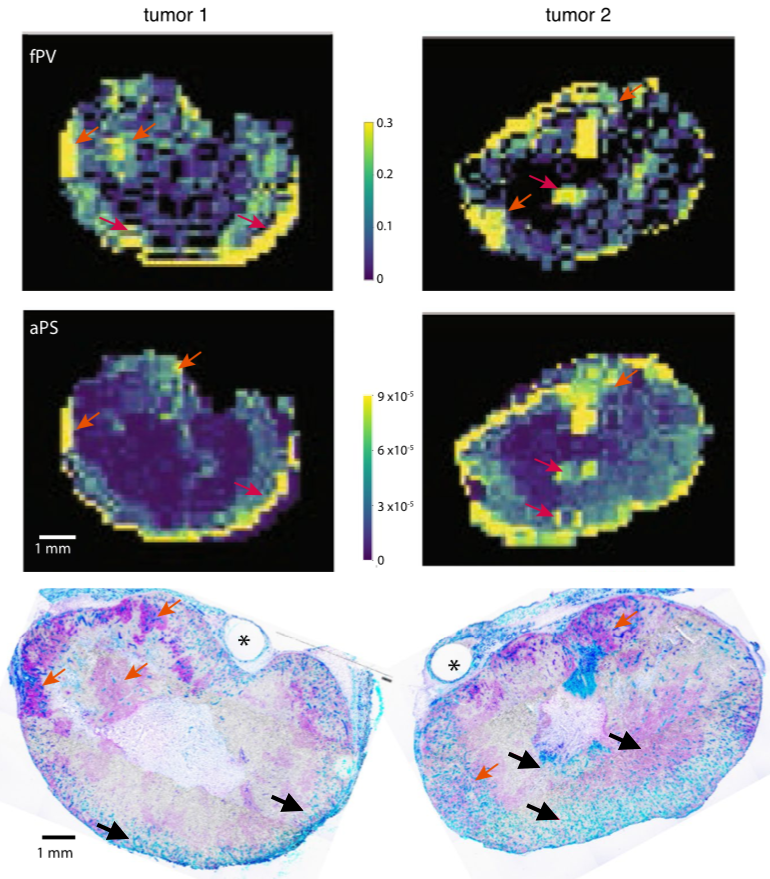
\includegraphics[width=\textwidth]{hpg/hpg-paper2-images/Fig6.png} 
  \caption{\acs{fPV} and \acs{aPS} parameter maps are compared to matched histology sections stained for bound trastuzumab (magenta), and for \acs{HER2} (grey), carbocyanine marker of perfusion (cyan) and for CD31 vasculature (blue). 
  Areas of vascular function (MRI) and trastuzumab (histology) correlation are indicated (orange arrows) in both modalities; example areas of poor matching are also shown (purple arrows). 
  Stars indicate location of fiducial markers for multi-modal slice comparison.}
  \label{hpgpaper2:fig6}
\end{figure}

\section{Discussion}

This study has shown direct evidence of poor trastuzumab access to metastases of the brain in a preclinical model.
Small clusters of cells that are immediately surrounded by highly perfused brain, liver or lung tissues may remain incompletely or in some cases totally unbound for trastuzumab.
Some avascular metastases of the brain may be outside the \acs{BBB} and therefore have poor access to trastuzumab, while larger lesions with active angiogenesis and blood vessel support may have a blood-tumour barrier (BTB) with greater trastuzumab delivery, however we have shown that microregional distribution of trastuzumab can remain highly heterogeneous and incomplete even when delivered by vessels within \acs{HER2}-positive lesions.
Our data are in agreement with other studies evaluating the permeability of brain metastases, which have found no correlation between metastases size, vessel density, aggressiveness or morphology and their permeability~\cite{Murrell:2015bz,Adkins:2016il}.
Mittapalli et al. have used mathematical modelling and MRI data to show a limit in the vascular pore size of MDA-MB-231-BR-\acs{HER2} metastases that would preclude access to \acs{MAb}s including trastuzumab~\cite{Mittapalli:2017iu}.
Other groups have also shown poor trastuzumab access in this model~\cite{Nounou:2016kl,TerrellHall:2017gu}.
As found here, trastuzumab has been detected in larger brain lesions in murine models~\cite{LewisPhillips:2017jj} where higher systemic doses of the \acs{MAb} were required to achieve anti-cancer efficacy seen for tumours grown in the mammary fat pad.
Accumulation over time has also been noted in patient metastases including those of the brain, where labeled antibodies were used for diagnostic purposes using PET~\cite{Dijkers:2010gc,Kurihara:2015kc}.
It is unknown if human tumours or metastases exhibit the same barriers to \acs{MAb} access.
As we have shown, access of trastuzumab to metastases and the distribution within can be highly heterogeneous, and is likely to be highly model and patient specific.
Ultimately, a majority of patients treated with trastuzumab eventually experience progression and relapse.
The rate of brain metastases has increased for \acs{HER2}-positive patients following treatment with trastuzumab, suggesting the \acs{MAb} therapeutic is less effective for tumours `behind' the \acs{BBB} than in metastases elsewhere such as the liver and lung~\cite{Stemmler:2006}.
Here we show direct evidence of poor trastuzumab access to \acs{HER2}-positive brain metastases and suggest that this confirms non-uniform access of \acs{MAb}s to cancers and metastases may be driving a significant portion of resistance to their effects.

Using tumour mapping analysis and \acs{DCE-MRI} we examined the impacts of tumour blood vessel architecture, vascular function and the tumour microenvironment on the patterns of distribution of trastuzumab in primary and metastatic models.
We observed that even when trastuzumab does have access to tumour tissues, the pattern of distribution is highly heterogeneous, similar to our previous work in a vector-overexpressing \acs{HER2}-positive breast cancer model~\cite{Baker:2008ci}.
Other groups demonstrating a limitation on the accumulation of trastuzumab in preclinical tumours have focused on net tumour accumulation and suggest that a major limitation to \acs{MAb} distribution is their difficulty distributing through the solid tumour tissue in the extravascular space~\cite{Jain:2010ie,Chauhan:2011fi,Lee:2010gb}.
In humans, \acs{MAb}s have a long half-life and are administered for many months.
The pharmacokinetic parameters of \acs{MAb}s are therefore thought to likely accommodate relatively slow distribution of \acs{MAb}s through the interstitium~\cite{Chauhan:2011fi,Thurber:2012dd}.
However, our 3D tissue disc data shows trastuzumab is able to diffuse relatively well through tumour tissues \emph{in vivo} in conditions of poor convective flow similar to an environment with high interstitial fluid pressure in vivo~\cite{Baker:2018ex}.
Neither is trastuzumab distribution limited by tight binding to antigen proximal to vessels as suggested by the binding-site barrier hypothesis~\cite{Juweid:1992ty}, as it reaches distances $>150 \mu$m from sources within 24h despite high \acs{HER2} expression~\cite{Baker:2018ex}.
This distance is similar to the diffusion limit for oxygen, therefore most tumour tissues are within this 150 $\mu$m range of a blood vessel and could be expected to have adequate exposure.
These data suggest that neither the binding site barrier hypothesis nor high interstitial fluid pressure adequately explain microregional variation in trastuzumab binding.
Given the incomplete access of trastuzumab seen in our models, other vessel- and tissue-level barriers appear to limit its distribution in the tumour microenvironment.

%One barrier to \acs{MAb} distribution appears to be the presence of tight junctions, labeled using ZO-1.
%However, these continuous barriers are not seen in vivo where inter-vessel heterogeneity occurs and even neighboring perfused vessels exhibit dramatic differences in the amount of bound drug on their perivascular cells.
Vascular maturity and architecture has also been attributed to poor drug access~\cite{Goel:2011ku}, however, no correlation between markers for aSMA or CIV and the relative distribution of trastuzumab has been found.
Higher doses and longer exposures do lead to higher numbers of vessels with perivascular trastuzumab, suggesting that some degree of intermittent perfusion or very poorly permeable vessels impact the observed microregional heterogeneity.
Non-perfused vessels have not been observed to have trastuzumab on perivascular cells, which suggests intermittent perfusion is an unlikely mechanism for observed inter-vessel heterogeneity.
Dynamic measurements of perfusion and permeability derived from DCE-MR imaging of high molecular weight contrast agent \acs{HPG-GdF} (583 kDa) suggest the intuitive relationship between vascular function and drug access is important, but does not consistently explain the heterogeneous patterns of drug distribution seen.
Areas of highly perfused tissue marked by carbocyanine in histological sections correspond to areas of high perfusion and/or permeability in MRI.
However, these tumour areas of high vascular function described in both imaging modalities may or may not have bound trastuzumab.
Similarly, regions with substantial amounts of bound trastuzumab do not necessarily correspond to areas of high perfusion or permeability measured using \acs{aPS} and \acs{fPV}.
HPG-GdF-derived parameters \acs{fPV} and \acs{aPS} arise under conditions that are closer to a permeability-limited regime than standard low-molecular weight contrast agents.
However, in the highly chaotic vascular environment of tumours we can still expect these MR-derived parameters of vascular function to not be completely independent of each other.

% All \emph{in vivo} models investigated were found to be sensitive to the effects of bevacizumab, a monoclonal antibody that binds VEGF-A and decreases vascular permeability~\cite{Ferrara:2005bk}.
% In our xenograft studies we see a dramatic reduction in the accumulation of trastuzumab in tumours when following pre-treatment with bevacizumab.
% The majority of tumour blood vessels cease to have extravasated trastuzumab bound to perivascular cells.
% These detailed images of the microenvironment highlighting reduced distribution at the vessel level agree with previous studies showing average reductions in trastuzumab delivery to the whole tumour~\cite{Arjaans:2013dv,Pastuskovas:2012dx}.
% In some cases VEGF ablation changes tumour vasculature, either the density or the fraction of perfused or mature vessels and the resulting overall function of tumour vasculature, but did not do so measurably in these tumours where neither the proportion of perfused vessels nor the amount of tumour hypoxia changed.

% The clinical impact of combination treatments is unclear, largely due to the difficulty in measuring drug distribution directly.
% Addition of bevacizumab did not improve outcomes for metastatic breast cancer patients being treated with docetaxel and trastuzumab~\cite{Gianni:2013hz}.
% Overall, poor clinical results have been found when combining VEGF ablation therapies with trastuzumab (reviewed in~\cite{Sledge:2015gb}).
% The potential risks of combining \acs{MAb}s and anti-angiogenic treatments have been recognized, and many publications and reviews in the pre-clinical and clinical fields of have called for investigations regarding optimal treatment and scheduling regimens for these combinations~\cite{Sledge:2015gb,Jain:2013jc,Chauhan:2012bm,Olson:2013go,Spector:2009gj,VanderVeldt:2014ii,LAM:2013dt}.

New strategies that are able to more effectively target and kill cancer cells, particularly metastatic disease, are urgently required.
Efforts to vary antigen-binding affinities and the size of \acs{MAb} fragments have been explored to improve their distribution through the extravascular compartment~\cite{Jain:2010ie,Chauhan:2011fi}.
Our data highlight the importance of also considering access of antibodies to target tumour tissues and whether microregional distribution of \acs{MAb} therapeutics may be affected when combined with vascular damaging agents or when targeting occult metastases.
Improvements to \acs{MAb} anti-cancer activity could be made in selection of combination therapies and the design of treatment schedules, as well as in the design of novel targeted drugs.
Efforts to examine these phenomena in the clinic would be of significant interest.

\section{Conclusions}
We have shown evidence for poor distribution and access of trastuzumab in preclinical tumours through direct visualization of bound drug, with particular implications for metastatic tumours, including those of the brain.
Our data suggest that the tumour microenvironment and tissue- and vessel-level barriers to drug distribution could effectively limit access of the drug to all its target cells.
These effects appear to be more important than slow interstitial distribution resulting from high interstitial fluid pressures or high binding affinity to \acs{HER2}.
Further, administering trastuzumab in combination with vascular disrupting agents could significantly impact its activity via reducing access.

\endinput
%% The following is a directive for TeXShop to indicate the main file
%%!TEX root = ../diss.tex

\chapter{Oxygen-enhanced MRI}
\label{ch:oemri1}

% ======================================================================
\section{Introduction}
% ======================================================================

Hypoxia is a well-established component of the tumour microenvironment, arising most often as tumour cell proliferation outpaces the growth of new vasculature.
Tumour hypoxia is an indicator of poor prognosis and is responsible for tumour resistance to radiotherapy and some chemotherapies, but is also a potentially useful target for novel anti-cancer drugs~\cite{Wilson:2011jp}.
Assessing tumour hypoxia in the clinical setting is challenging largely due to the invasive nature of biopsy-dependent techniques and the limited capacity and high expense of the more favoured, non-invasive PET imaging of hypoxia tracers~\cite{Horsman:2012kw}.
The utility of screening patients for hypoxia was demonstrated retrospectively in trials of the hypoxic cytotoxin tirapazamine, where those patients with greater PET-imaged hypoxia experienced greater benefit~\cite{Rischin:2006fz}.
However, subsequent trials of drugs targeting hypoxia, including those for evofosfamide that failed to show clinical benefit, have not used hypoxia imaging to stratify patients.
A practical, widely applicable, and non-invasive imaging method is urgently required as a biomarker to monitor tumour hypoxia in many contexts, and is crucial to the development and clinical evaluation of future hypoxia-targeting drugs.

% this used to be the interlude
% START of the interlude
\section{Theory}
\subsection{Physiology}
The primary mode of oxygen delivery to tissue is the haemoglobin (\acs{Hb}) molecule as it carries and delivers 98\% of the oxygen in the body. 
Over 250 million \acs{Hb} molecules are found in a typical red blood cell and each \acs{Hb} molecule has four binding sites for oxygen molecules. 
The binding affinity for ${O_2}$ drastically increases for subsequent oxygen molecules that bind to \acs{Hb} as the conformation of the \acs{Hb} molecule changes to increase binding affinity for the next oxygen, a phenomenon called cooperativity. 
Similarly, when the local environment of the \acs{Hb} molecule changes such that O$_2$ needs to be released, the reverse conformational changes occur; a proportionately lower drop in oxygen tension is then required to release the next O$_2$ molecule. 
The dissociation of oxygen from haemoglobin molecules is well described by the oxygen-haemglobin dissociation curve (figure~\ref{HBdis}).

\begin{figure}
 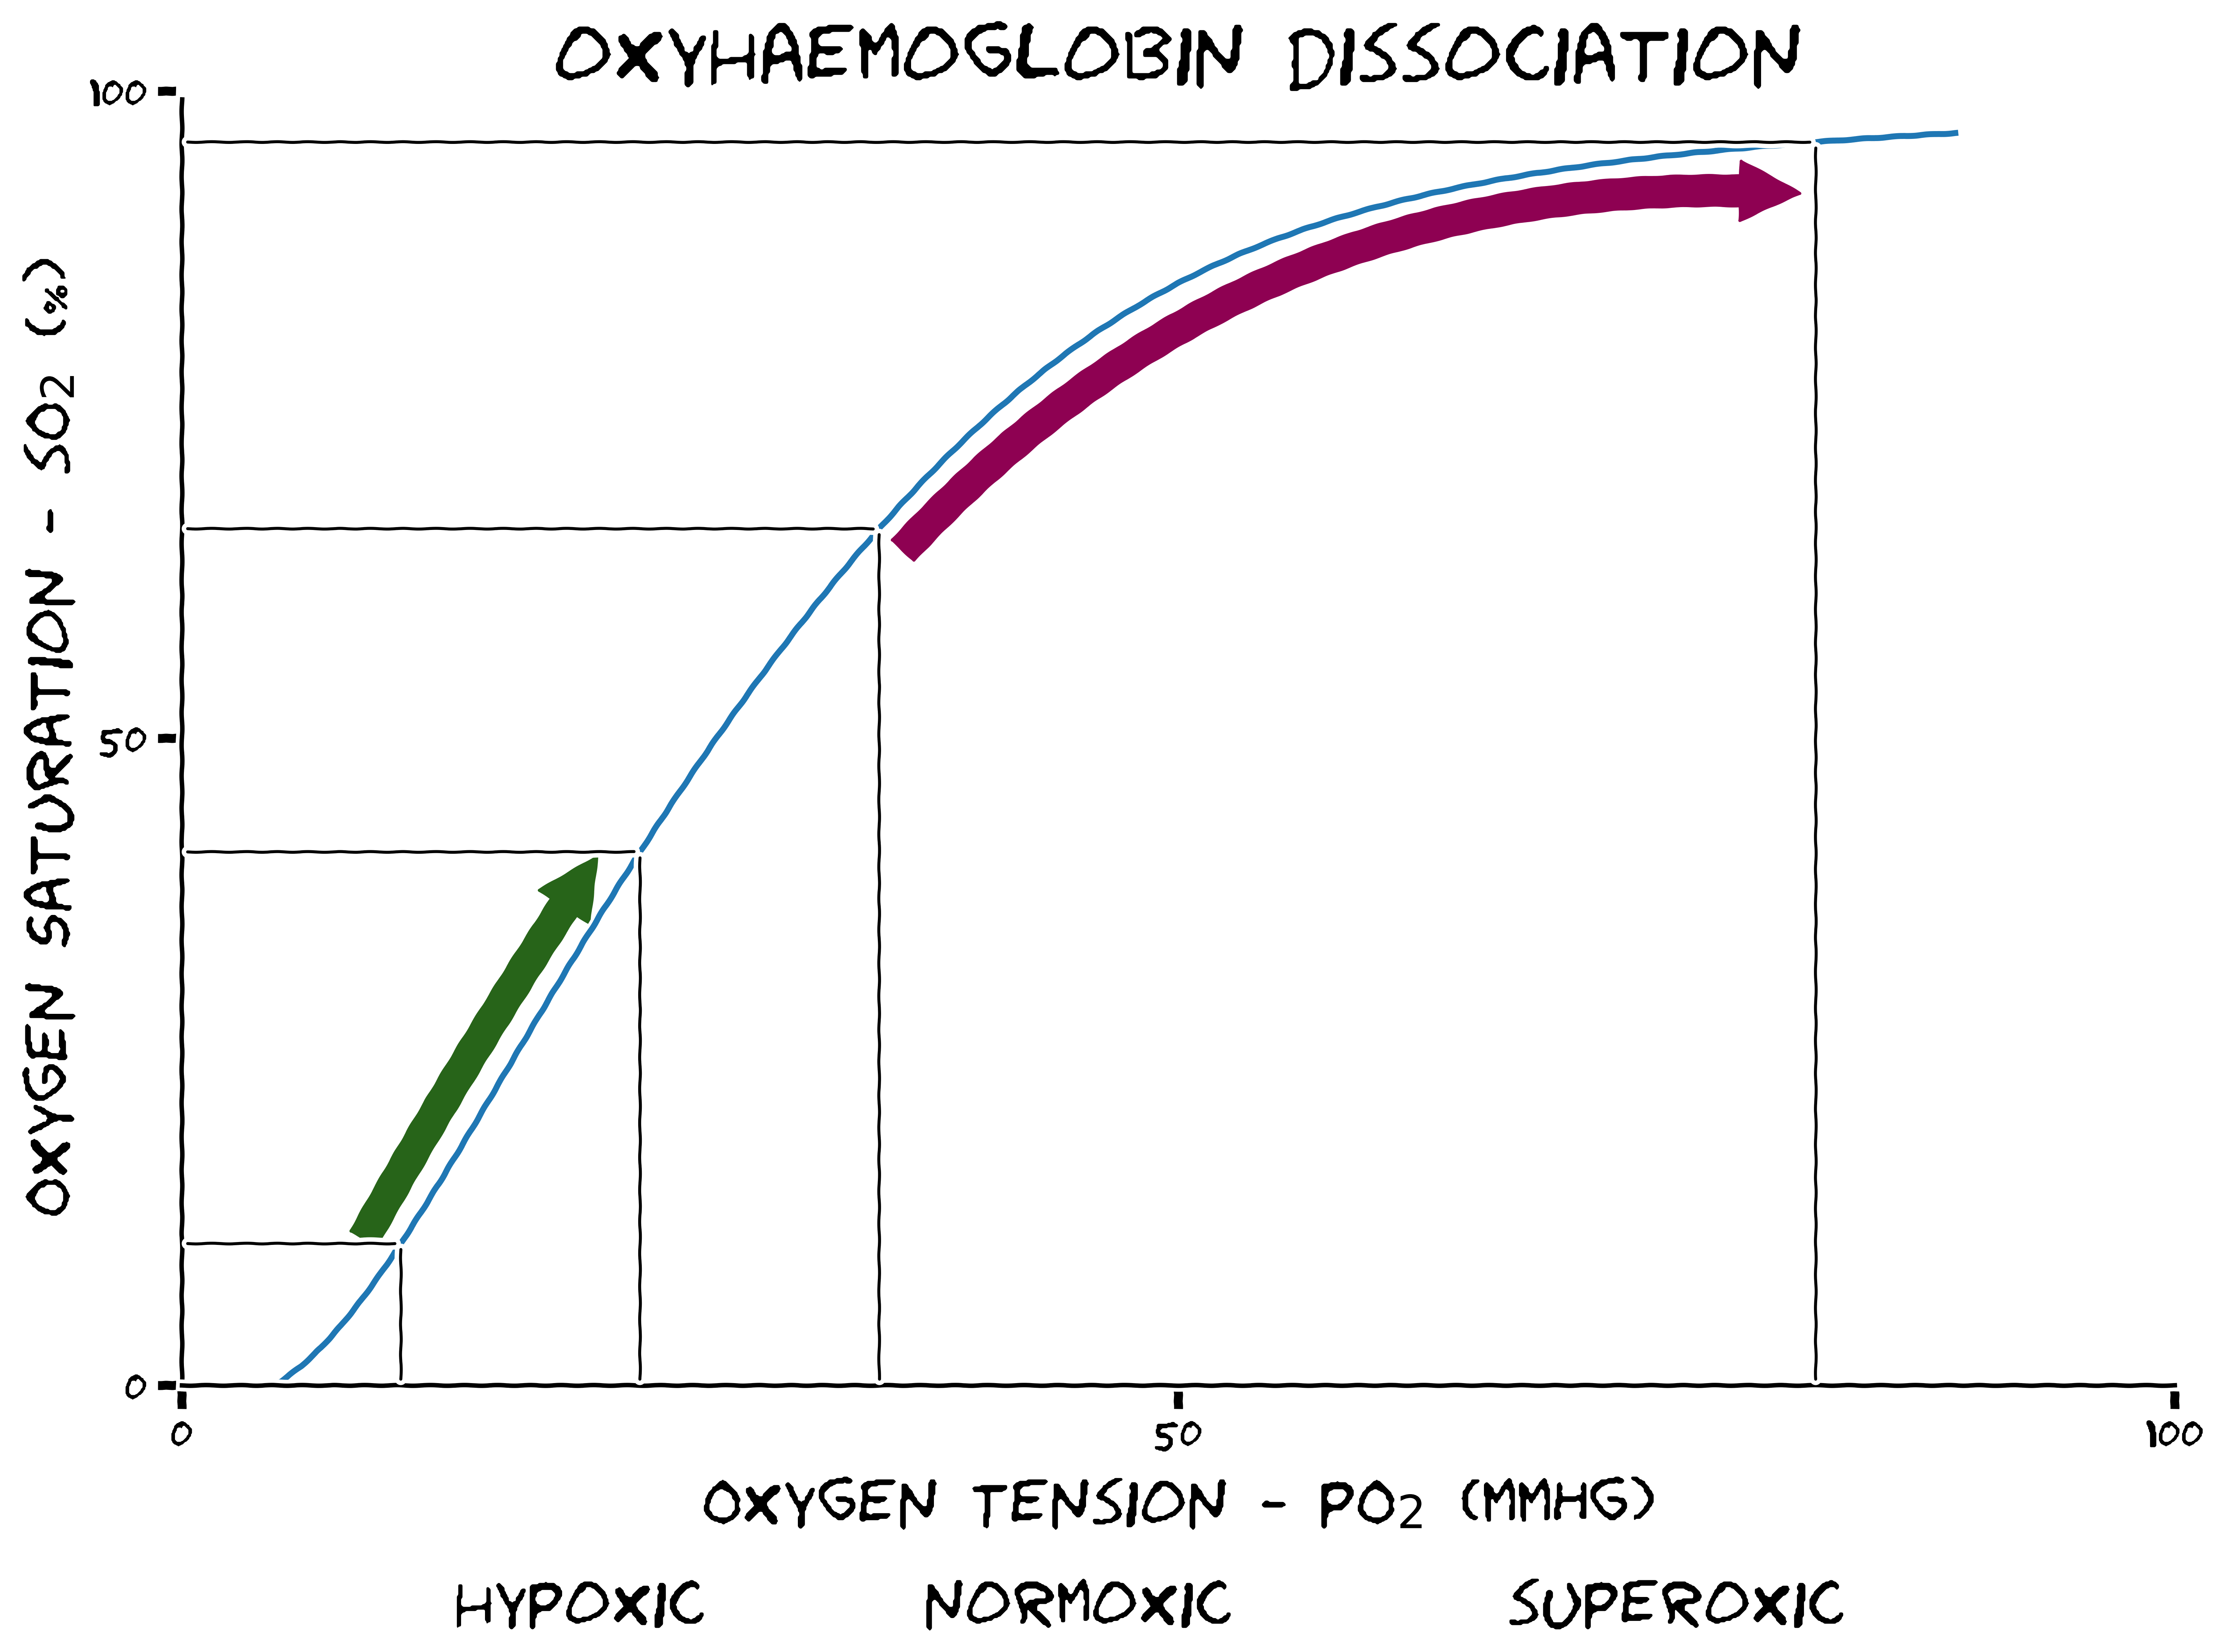
\includegraphics[width=\textwidth]{./oemri_thesis1/oemri_thesis1-images/Hbdissociation.png}
 \caption{Sigmoidal curve illustrating the relationship between the haemoglobin saturation (y-axis) and the oxygen tension (x-axis). When the oxygen tension is low, the Hb easily binds $O_2$ and there is a rapid rise in oxygen saturation (green arrow). Note that it takes a large increase in oxygen tension to bind the last O$_2$ and similarly, a large decrease in oxygen tension to release the last O$_2$ (purple arrow) ~\cite{GomezCambronero:2001hu}.}
 \label{HBdis}
\end{figure}	

Upon inspiration of atmospheric air (p$_{O_2}$ = 160 mmHg), gas exchange in the pulmonary capillary beds occurs in the alveoli of the lungs (Figure~\ref{mmhg}).
Incoming venous blood with a low oxygen tension ($p_{O_2}$ = 40 mmHg) is oxygenated as haemoglobin molecules readily bind available oxygen. 
As the oxygenated blood leaves the alveoli and moves through the systemic arteries, it has an oxygen tension of 100 mmHg. 
The oxygenated blood then travels from the arteries to the systemic capillary bed and the local oxygen tension drops from 100 to 40 mmHg.
Simultaneously, while the \acs{Hb} molecule undergoes a structural change releasing a molecule of O$_2$ from its first binding site.  
The second release of the oxygen molecule occurs when the tension drops to 26mmHg~\cite{GomezCambronero:2001hu}.
In a population of \acs{Hb} molecules fully saturated in tissue (S$_{O_2}>95\%$), the approximate $\Delta pO_2$ required to release the first ${O_2}$ molecule is 60 mmHg (100-40 mmHg).
The third ${O_2}$ molecule is released when the $pO_2$ drops from 26 to 19 mmHg, and the final ${O_2}$ molecule is released when the $pO_2$ drops to 12 mmHg~\cite{GomezCambronero:2001hu}.
Practically however, it is important to note that \acs{Hb} molecules never release all four of the bound oxygen \emph{in vivo}.
This important feature of \acs{Hb} (cooperativity) ensures that small changes in p$_{O_2}$ have the appropriate effect in the appropriate place. 
For instance, in the lung tight binding is required so \acs{Hb} can bind the O$_2$ needed to supply all the tissues.
Therefore, small changes should not affect the release of O$_2$.
Conversely, small changes in p$_{O_2}$ in capillary beds should result in quick release of O$_2$ so it can easily diffuse to oxygen-starved tissues. 

\begin{figure}
    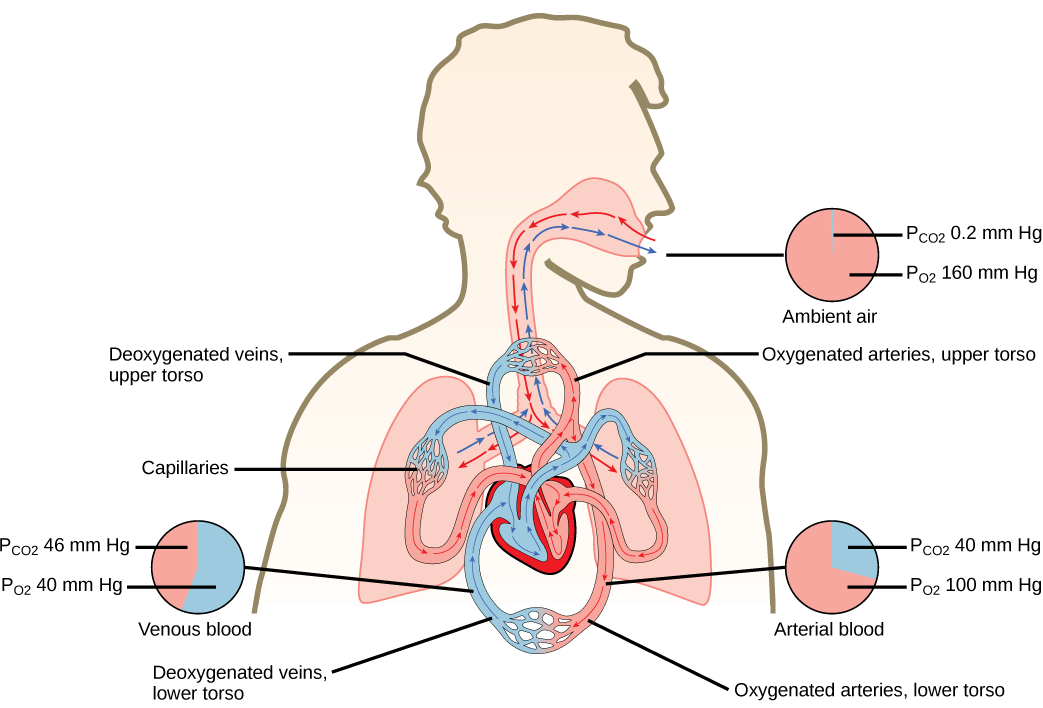
\includegraphics[width=0.8\textwidth]{./oemri_thesis1/oemri_thesis1-images/mmHg.png}
    \caption{A schematic of the change in the partial pressures of oxygen and carbon dioxide at various points in the body.
    The $p_{O_2}$ of inhaled ambient air is 160 mmHg, and this is breathed in to the lungs.
    Oxygen diffuses out of the alveoli into the surrounding capillaries and binds to Hb due to the pressure gradient (capillary $p_{O_2}$ is 40 mmHg).
    This oxygenated blood ($p_{O_2}$ = 100mmHg) now enters the heart and is pumped through the body, with the Hb releasing oxygen through capillaries due again to the pressure gradient (tissue $p_{O_2}$ is $<$ 40 mmHg)~\cite{OpenStaxBio:2016uu}. 
    Textbook content produced by OpenStax Biology is licensed under a \href{https://creativecommons.org/licenses/by/4.0/}{CC-BY 4.0 license}.}
    \label{mmhg}
\end{figure}

\subsection{Origin of the OE-MRI signal}

Oxygen is a paramagnetic molecule because it has two unpaired electrons and it is widely reported that the dominating effect in the OE-MRI signal is a T$_1$ decrease after concentrated oxygen gas (100\% O$_2$) is breathed in~\cite{OConnor:2016ee,Linnik:2013hf}. 
The excess oxygen travels through the blood stream dissolved in plasma and diffuses through the vessel walls and dissolves in interstitial tissue fluid (figure~\ref{oemri}).
The net increase in dissolved oxygen results in a dramatic and measurable decrease in T$_1$. 
This change is reversed soon after the patient is switched back to breathing atmospheric air as excess oxygen is expelled or metabolized. 
Perfused tumour regions (i.e regions that already have a high \acs{Hb}-O$_2$ saturation) will see a measurable decrease in T$_1$. 
The perfused regions that do not show a decrease in T$_1$ must therefore be hypoxic~\cite{OConnor:2016ee}. 
Importantly, OE-MRI does not yield any information about unperfused regions and in that region, there are likely to be pockets of viable (but hypoxic) tissue.

The oxygen status of healthy tissue is fairly well regulated in normal tissue and every cell in the body is at most 150$\mu$m away from a blood vessel. 
In tumours however, the vascular network is chaotic and the growth patterns of vessels are abnormal leading to a defective and leaky endothelium~\cite{McDonald:2002ut}. 
Irregular diameters of tumour vessels, abnormal branching patterns and porous vessel walls all contribute to an increase in vessel permeability and pockets of hypoxic tissue. 
Although $pO_2$ and $pCO_2$ are by far the largest factors in determining Hb staturation, related factors such as pH and temperature also play a role.
Furthermore, these hypoxic regions are heterogeneous, transient, and drastically differ between tumour models. 
In a mammary adenocarcinoma mouse tumour model, Sorg et al. used spectral imaging with an implanted window chamber to show that upon breathing 100\% oxygen, the \acs{Hb} saturation in the tumour vascular network increases from 20-30\% up to 70-80\% while the \acs{Hb} saturation in the normal vascular network does not change appreciably~\cite{Sorg:2008eg}.

\begin{figure}
	\begin{center}
	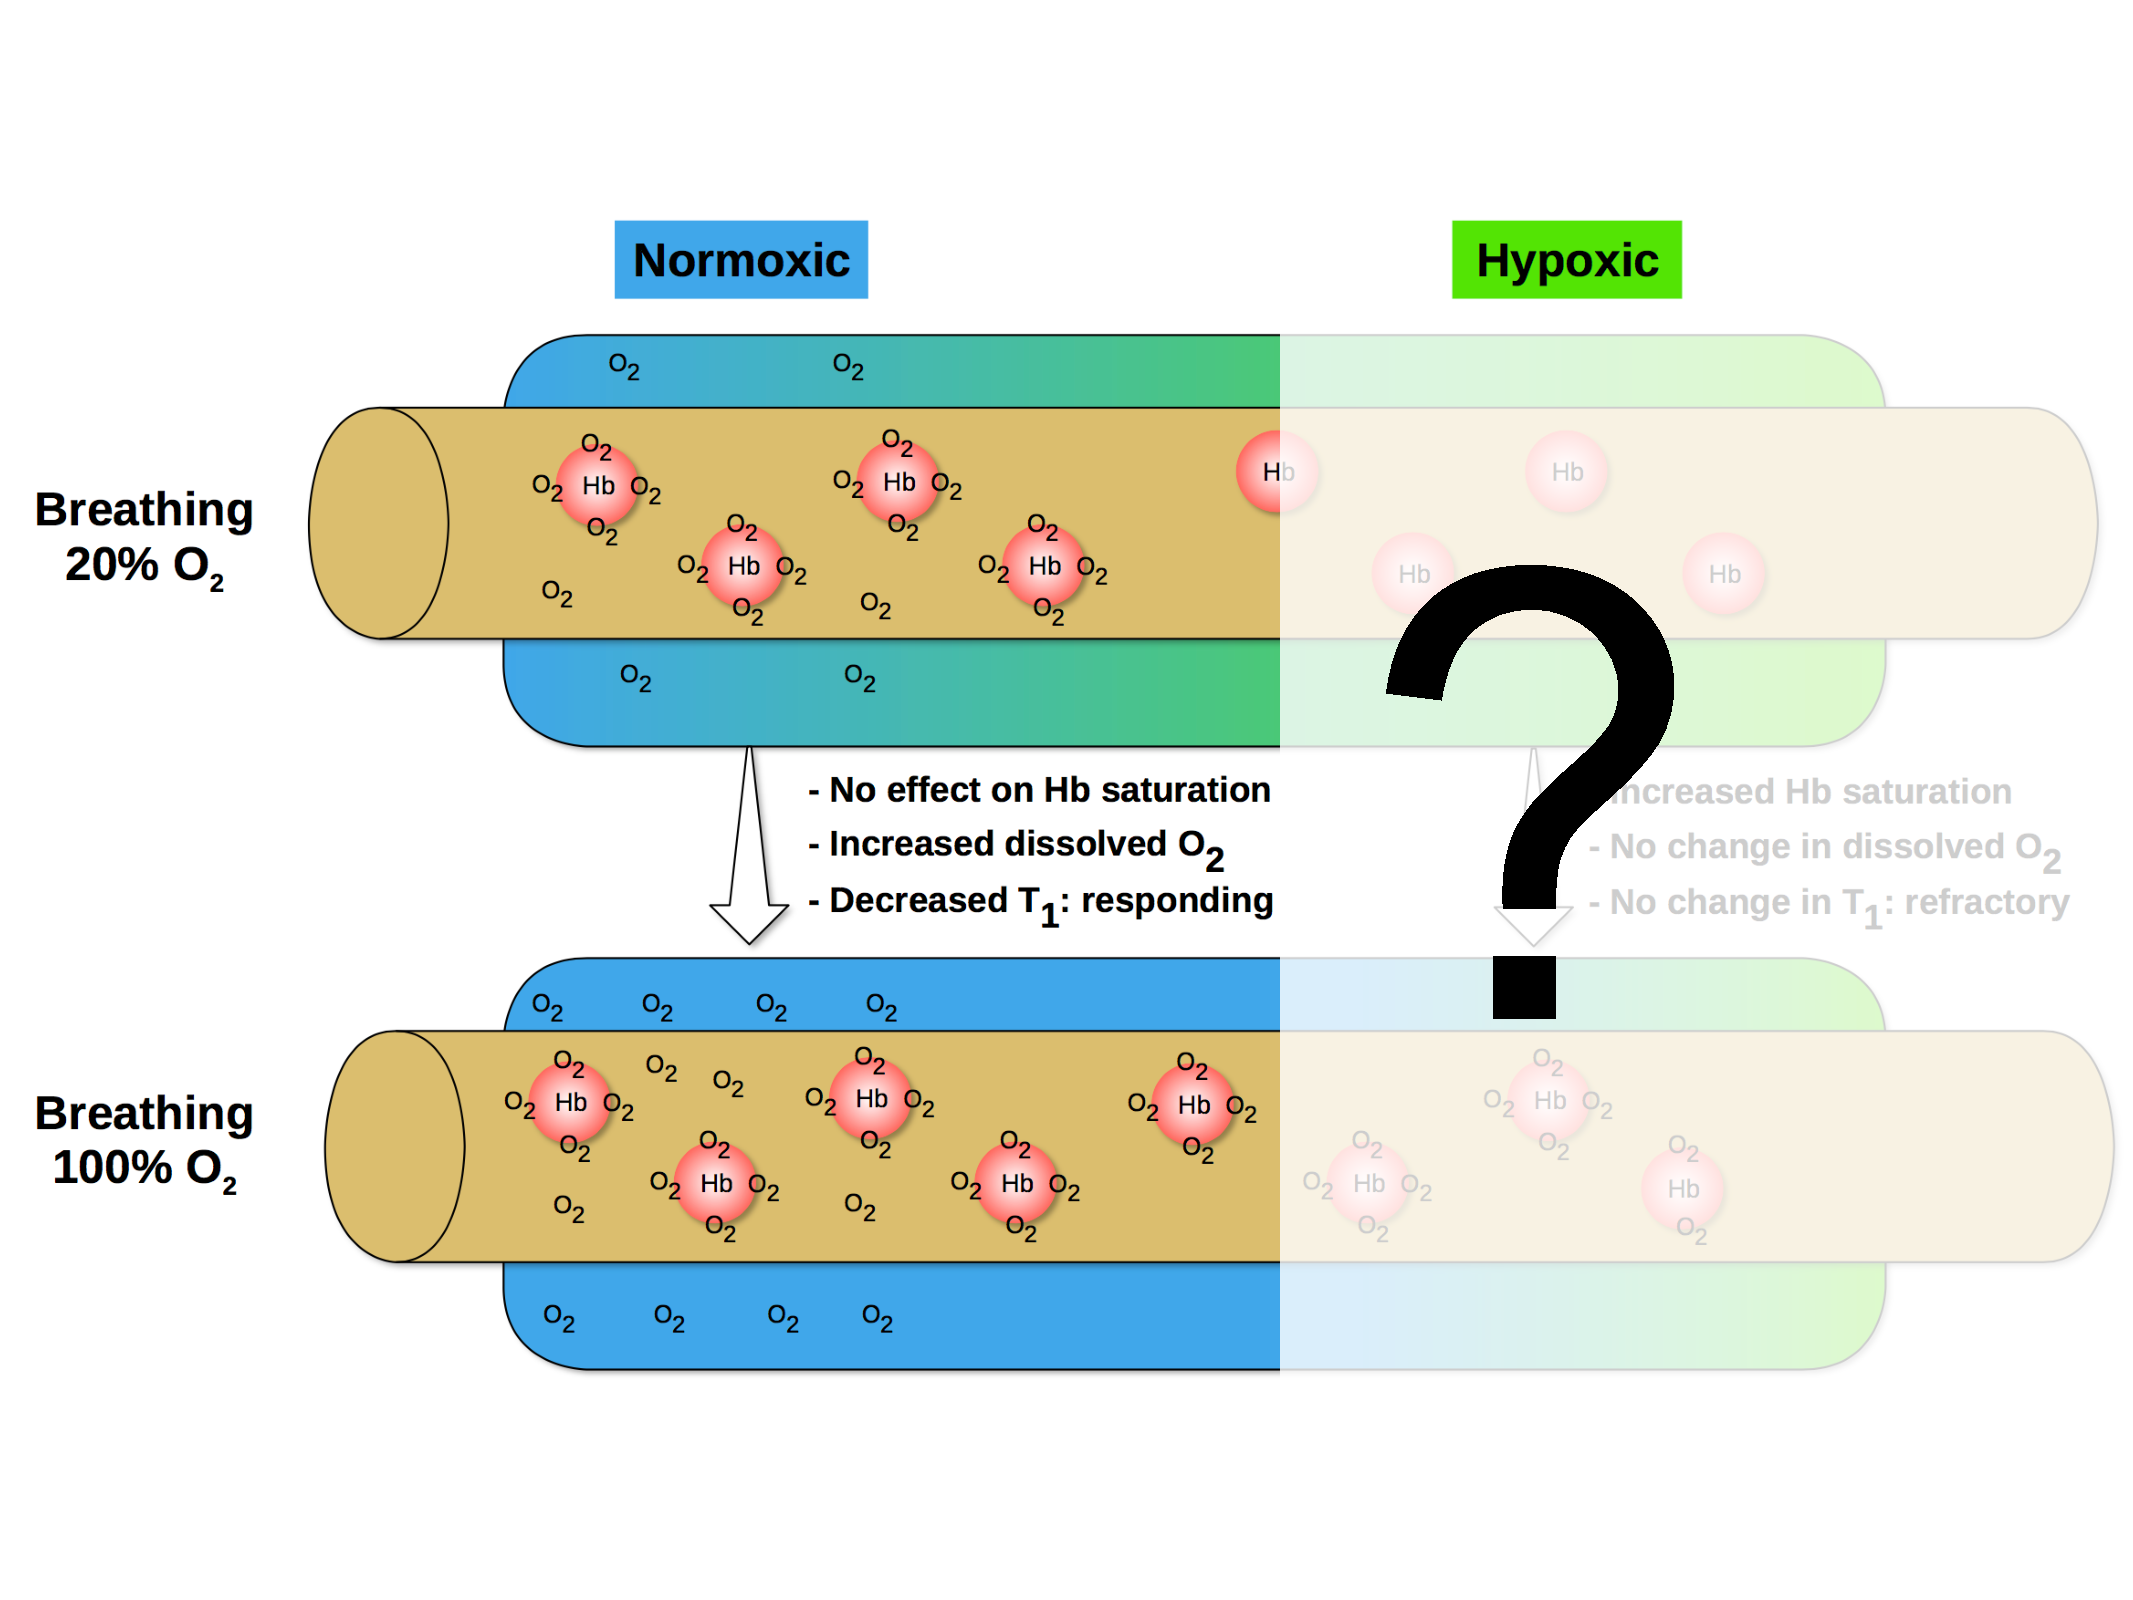
\includegraphics[width=\textwidth]{./oemri_thesis1/oemri_thesis1-images/oemriDark.pdf}
	\caption{A schematic representation of our current understanding of the origin of the OEMRI effect. In normoxic tissue, \acs{Hb} is almost fully saturated and any excess breathed O$_2$ cannot bind to the \acs{Hb} molecule. Consequently, O$_2$ dissolves in the blood plasma and as the excess oxygen diffuses out into the tissue, it also dissolves in the interstitial tissue fluid resulting in a net T$_1$ decrease. It is hypothesized that in the hypoxic tissue, \acs{Hb} is not fully saturated with oxygen due to increased tissue demands and/or a poorly organized vascular network. The excess breathed oxygen in this case binds to the \acs{Hb} molecule and does \textbf{not} dissolve in the plasma leading to no change in T$_1$.}
	\label{oemri}
	\end{center}
\end{figure}
% End of the interlude

\section{Motivation}

The T$_1$-shortening property of oxygen dissolved in fluid has been known since 1955~\cite{Chiarotti:1955kf} and pioneering work by Young et al. showed that oxygen acts as a paramagnetic contrast agent by demonstrating its ability to reduce T$_1$ upon inhalation~\cite{Young:1981vf}. 
Inhalation of 100\% oxygen has also been shown to elicit strong T$_1$ effects in the kidney\cite{Jones:2002dh}, spleen\cite{Tadamura:1997vc} and the poorly oxygenated retina~\cite{Berkowitz:2001uz}. 
Subsequent oxygen-enhanced MRI (OE-MRI) efforts have included either acquisition of quantitative T$_1$ maps before and after oxygen breathing, or acquiring dynamic T$_1$-weighted (T1W) signal intensity images and calculating $\Delta$T$_1$ during periods of oxygen inhalation.
The subtle but measurable influence of tissue oxygenation on T$_1$ in tumours has been reported by O'Connor~\cite{OConnor:2016ee,OConnor:2009ku,OConnor:2009bp,Little:2018iu}, Mason~\cite{Zhao:2015ez,White:2016fz,Hallac:2014cb}, Gallez~\cite{Jordan:2012do}, and others~\cite{Tadamura:1997vc,McGrath:2008kx,Kershaw:2010ha,Linnik:2013hf}. 
However, due to the changes in T$_1$ that arise as oxygen dissolves in the plasma and interstitial fluid being quite small, T$_1$ maps have poor sensitivity and application of OE-MRI techniques in cancer has yielded mixed success.
OE-MRI continues to suffer from low \acs{SNR} and it has not found routine clinical use largely because isolating small signal changes due to dissolved O$_2$ is a challenge~\cite{OConnor:2016ee, Zhao:2015ez}.

Typical imaging times for existing OE-MRI methods range from 20-45 minutes often making it impractical for easy inclusion in experimental protocols. 
An MRI technique measuring tumour oxygenation that is sensitive, fast, flexible, repeatable, and non-invasive has the potential to significantly impact the clinical fields of radiation biology and hypoxia drug targeting.
In this study, we present a new dynamic OE-MRI (dOE-MRI) method that allows extraction of very small dynamic signal changes in T$_1$W images by inducing step changes in the inspired oxygen through a repeated, cycling gas challenge.
To isolate the signal component that matches cycling gas, a blind source separation approach called independent component analysis (\acs{ICA}) is used to analyze MR images as first proposed by McKeown at al~\cite{McKeown:1998wo}.
\acs{ICA} is a form of blind source separation algorithm that separates the additive signals on the basis of the statistical independence of individual components~\cite{Hyvarinen:2000vk}.
With the application of a cycling oxygen challenge and processing the data using \acs{ICA}, our \acs{dOE-MRI} approach represents a significant improvement in the sensitivity and application of MRI for measuring tumour oxygenation, making it more practical for wide application.
% ======================================================================
\section{Methods}
% ======================================================================
\subsection{Mice and tumours}

Female NRG (NOD rag gamma) mice were implanted with murine squamous cell carcinoma (SCCVII; 5x10$^5$ cells in 50 $\mu$l serum-free media; cells provided by Dr.\ J. Evans) in the dorsal subcutaneous region.
Mice were anaesthetized with isoflurane for the duration of imaging sessions until euthanasia, and were positioned supine on the custom surface coil apparatus.
Throughout the imaging session, a small animal monitoring system (SA Instruments Inc., Stony Brook, NY, USA) was used to monitor respiration rate, varying between 80-100 breaths per minute, and body temperature, maintained at $36.8 \pm 0.5^\circ$C using a continuous airflow heater.
All animals were injected with 60~mg/kg pimonidazole hydrochloride (HypoxyProbe) 30~min prior to imaging to label hypoxic cells and were euthanized within 15~min of imaging completion.
Tumours were embedded and frozen in optimum cutting temperature medium (OCT; Tissue-TEK).

%\subsection{Immunohistochemistry, image acquisition and analysis}
%Co-planar MRI slices and histological sections were obtained by imaging perpendicular to the longest tumour axis in MRI and serial-step 10 $\mu m$ cryosections were cut at 0.5-mm intervals in the same plane.
%Slides were then fixed in acetone-methanol for 10-min and whole sections were immunohistochemically stained~\cite{Kalra:2017is} for CD31 (PECAM; visualized using secondaries labeled with Alexa 647nm) to label blood vessels, and for pimonidazole (HypoxyProbe-1; visualized using secondary labeled with Alexa 546nm) to label hypoxic cells. Sections were then stained using Hoechst 33342 (bisbenzimide) to label all cell nuclei.
%Whole-tumour sections were imaged using a robotic fluorescence microscope (Zeiss Axioimager Z1), a cooled, monochrome CCD camera (Retiga 4000R; QImaging), a motorized slide loader and x-y stage (Ludl Electronic Products) and customized ImageJ software~\cite{Collins:2007jr}. 
%Adjacent microscope fields of view were tiled such that images of entire tumour cryosections were captured at a resolution of 1.5 $\mu m$/pixel. 
%Using anatomical landmarks and accumulated thicknesses of serial-step sections as estimates of distances from the edges of whole tumours, sections were chosen to match the MR slices. 
%ImageJ and user-supplied algorithms were used to super impose digital images which were then manually cropped to tumour tissue boundaries with staining artifacts removed. A threshold was applied to images to identify positive pimonidazole staining, and the number of positive pixels was determined as a percentage of the total number of pixels in the tumour image. The histological hypoxic fraction is reported in the highly necrotic HCT-116 tumours as the percentage of pimonidazole+ pixels summed with the percentage of necrotic pixels, as this value should most closely approximate the MR imaging data that does not discriminate between these regions; SCCVII tumours do not have necrosis and so the same value is reported as the percentage of pimonidazole+ pixels.
%Overlaid greyscale images were converted to false color for visualization with pimonidazole as green and CD31 as magenta. 

\subsection{MRI data acquisition}
\label{doemri_mrianalysis1}
All MRI experiments were performed at the UBC MRI Research Centre on a 7T Bruker BioSpec 70/30 scanner at room temperature with a volume transmit coil and custom surface receive coil.
Each imaging session began with pilot axial and coronal T$_2$-W scans for tumour localization and slice prescription.
Eight contiguous axial slices (1~mm thickness) were acquired with an in-plane field of view of 3.84~cm$\times$1.92~cm and a matrix size of 128$\times$64.
Dynamic oxygen-enhanced MRI (dOE-MRI) scans were acquired with a 2D multi-slice FLASH-based sequence with T$_E$/T$_R$ = 2.67/66.7, $\alpha=40^\circ$, temporal resolution of 4.3~s with 198 repetitions for a total scan time of about 14~min.
The spatial resolution and geometry for all scans in the imaging session were matched and an experienced operator outlined the tumour on each slice of the anatomy MR images to construct the region of interest (ROI) for each animal.

\noindent\textbf{Gas challenge during MRI:} tumour-bearing mice began the \acs{dOE-MRI} gas challenge breathing medical air and were switched between 100\% oxygen and medical air in two-minute intervals.
This paradigm continued for three cycles over a total of fourteen minutes; gases were switched manually and each switch took about five seconds to complete.

\subsection{MRI data analysis}
\label{doemri_mrianalysis2}
\textbf{dOE-MRI maps:} A suite of in-house software was developed based on the technique described by Hyvarinen~\cite{Hyvarinen:2000vk}.
Specifically the python machine learning library scikit-learn, \texttt{sklearn.decomposition.FastICA}, was used~\cite{Pedregosa:2011tv}.
The Fast\acs{ICA} algorithm is applied to serially acquired T$_1$W images and the output is a paired set of components and weighting factors for each voxel in the dataset.
Extracted independent components are not ordered and while the component selection can be automated, in this study an observer was assigned to select the appropriate component (Figure~\ref{technique}).
The number of independent components for each imaging session was chosen by the operator and ranged from 4-9 to ensure the cyclic behaviour of the T$_1$W signal intensity corresponding to the gas challenge appeared in only one component. 
The \acs{dOE-MRI} maps were obtained by dividing the \acs{ICA} weighting-factor maps by the mean signal-intensity maps to obtain a spatial map for the strength of a particular voxel's contribution to the component of interest ($c_4$ in Figure~\ref{technique}).
In these \acs{dOE-MRI} maps, voxels are coloured to indicate the amount by which a given pixel intensity timecourse is modulated by the oxygen-related component.  
The green-white-purple colour spectrum depicts the degree to which voxels respond to the cycled gas challenge.
Purple indicates O$_2$-positive voxels whose timecourse exhibits a higher and more positive contribution from the corresponding \acs{ICA} component, representing an increase in T$_1$W signal intensity in response to the supplied 100 \% oxygen. 
O$_2$-negative voxels that show a decrease in T$_1$W signal intensity with a negative contribution from the corresponding \acs{ICA} component under 100 \% oxygen breathing are depicted as green. 
Regions whose T$_1$W signal intensity timecourses responds only weakly or not at all to the gas challenge are shown in white hues.
Fraction of voxels that are negative on \acs{dOE-MRI} maps were correlated with the histological hypoxic fraction using Pearson's r.

\noindent\textbf{OE-MRI without \acs{ICA}:} To assess whether or not \acs{ICA} was necessary to create oxygenation maps, the MR signal intensity data was correlated with two modeled paradigms: 1) a square wave which corresponds to the concentration of delivered oxygen; 2) a synthetic hemodynamic response function (HDRF) created by convolving a square wave with an exponential ($\tau=0.32$ms).
The value of $\tau$ was determined by manually fitting a portion of the ICA-extracted oxygen-enhancing component to the HDRF with a range of $\tau$ values.
Correlations were calculated voxel by voxel using:

\begin{equation}
r = \frac{\Sigma^n_{i=1} (x_i - \bar{x}) (y_i - \bar{y})}{\sqrt{\Sigma^n_{i=1} (x_i - \bar{x})^2 \Sigma^n_{i=1} (y_i - \bar{y})^2}}
\end{equation}
where $x$ is the model paradigm and $y$ is the T$_1$W signal intensity timecourse.
The resulting correlation maps are estimates of the strength of the input paradigms with the acquired signal intensity.

% ======================================================================
\section{Results}
% ======================================================================

\subsection{\texorpdfstring{\acs{ICA}}{ICA} isolates small changes in \texorpdfstring{T$_1$}{T1}W signal intensity}

An example signal intensity vs.\ time curve is shown for a whole slice ROI compared with a single voxel (Figure~\ref{technique}B).
A mean signal intensity increase is seen for both the whole slice and the individual voxel during each of the oxygen periods of the cycle, however the magnitude of $\Delta SI$ for the individual voxel is about 10\% and the noise is of the same order of magnitude.
The slice-averaged timecourse has much less noise compared to the individual voxel, but the size of the effect is significantly reduced, the contrast to noise is similarly poor, and all spatial heterogeneity in the response is lost in the averaging process.

To retain spatial information and improve the sensitivity of the technique, \acs{ICA} was applied to the same dataset and in this example, four independent components were extracted (Figure~\ref{technique}C). 
Each individual independent component is scaled such that its norm is one ($||c_i||=1, \forall i $).
Only one extracted component follows the step function of the oxygen challenge and positively identifies an effect of oxygen breathing (c$_4$).
Speculations for the source of the other components is provided in Figure~\ref{Sfig_components}.
\begin{figure}[htbp]
   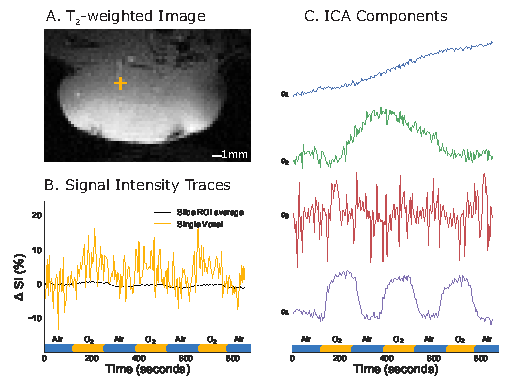
\includegraphics[width=\textwidth]{oemri_thesis1/oemri_thesis1-images/fig1_technique.pdf} % requires the graphicx package
   \caption{(A) T$_2$W MRI of a tumour xenograft at 7T and (B) the corresponding T$_1$W signal-time traces of a single voxel (solid yellow) and whole-tumour slice ROI (dotted black) during gas cycling at two-minute intervals of air (x axis; blue) and O$_2$ (x axis;yellow).
(C) Plot of the four extracted \acs{ICA} components from the entire tumour ROI, component \textbf{$c_4$} (purple) exhibits the same temporal features as the oxygen cycling time course shown along the bottom. All components are normalized, no vertical scale is shown.}
   \label{technique}
\end{figure}

\subsection{dOE-MRI with \acs{ICA} does not require assumption of a response function}
To determine whether \acs{dOE-MRI} maps obtained with a model-free \acs{ICA} approach (Figure~\ref{fig_correlation}A) are comparable to maps assuming mathematical models of the response, alternative oxygenation status correlation maps were constructed (Figure~\ref{fig_correlation}B and C). 
In Figure~\ref{fig_correlation}B and C, two example mathematical models - a square wave and the estimated hemodynamic response function (HDRF) - are correlated to the voxel-by-voxel raw time signal. 
Regions most correlated with the input paradigm remained purple in both alternative maps generated from modelled response functions.
Particularly when using the HDRF, the alternative oxygenation map showed very similar patterns in the regions demarcated as O$_2$-positive and O$_2$-negative. 
However, the map generated from correlating a square wave led to consistent underestimation of oxygenation relative to the model-free \acs{dOE-MRI} map.

\begin{figure}[htbp]
   \centering
   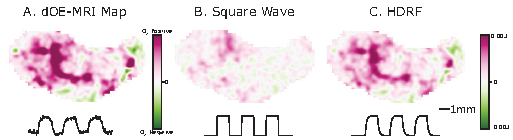
\includegraphics[width=\textwidth]{oemri_thesis1/oemri_thesis1-images/fig3_correlation.pdf} % requires the graphicx package
   \caption{(A) \acs{dOE-MRI} map of an SCCVII tumour where purple voxels contribute strongly to the extracted component using \acs{ICA} in the T$_1$W signal timecourses. 
Green voxels in the \acs{dOE-MRI} map have a strong contribution of the inverse extracted component. Pearson's r-maps are shown correlating the raw time-signal voxel by voxel with a square wave (B), and an exponential convoluted with a square wave called the hemodynamic response function (HDRF) (C).
Panels B and C are correlation maps whereas A is the \acs{dOE-MRI} map from \acs{ICA}. Note the low correlation coefficients (on the order of $10^{-3}$) are characteristic of the extremely low amplitude of the oxygen cycling compared to other competing effects.
   \label{fig_correlation}}
\end{figure}

\subsection{Variability of response in individual oxygen cycles}

A full \acs{dOE-MRI} sequence involved three cycles of oxygen but to assess the potential for shortening the sequence we also separately applied \acs{ICA} to each of the three oxygen cycles independently.
Separate \acs{dOE-MRI} maps, as well as voxel-wise correlation plots of a representative SCCVII tumour, are shown in Figure~\ref{fig_repeatability} with Pearson's r$_{all-1}$=0.74,r$_{all-2}$=0.86,r$_{all-3}$=0.84.
Pearson's r ranged from 0.79 to 0.87 for a similar analysis in a representative HCT-116 tumour.

The stability of the independent component extraction was assessed by undersampling the full timecourse threefold prior to application of \acs{ICA}, and a high correlation between the \acs{dOE-MRI} maps from full and three-fold undersampled timecourses is observed (Figure~\ref{fig_repeatability}E; Pearson's r = 0.84). 
In Section~\ref{sec:interleave}, further undersampling up to a factor of six is shown with minor differences in the \acs{dOE-MRI} map.

\begin{figure}[htbp]
   \centering
   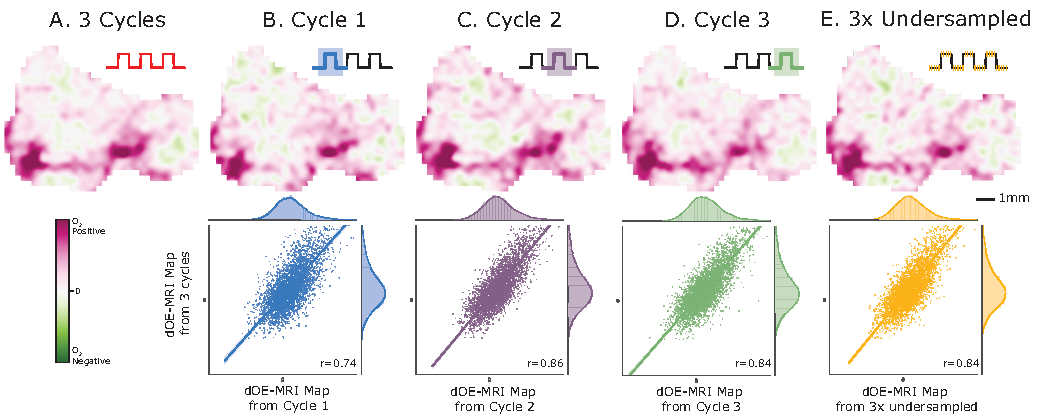
\includegraphics[width=\textwidth]{oemri_thesis1/oemri_thesis1-images/fig4_repeatability.pdf} % requires the graphicx package
   \caption{The \acs{dOE-MRI} map including the full dataset of all three cycles (A) is compared to each of the three gas cycles separately (B,C,D), and to a map that temporally undersamples by selecting every third datapoint from the full dataset (E).
Voxel-wise plots of each map are correlated to the full dataset and a linear regression with Pearson's r is shown.
   \label{fig_repeatability}}
\end{figure}

\subsection{dOE-MRI can be extended by interleaving other scans between each repetition}
\label{sec:interleave}
To investigate the subsampling limit of \acs{ICA}, Figure~\ref{subSample} shows the \acs{dOE-MRI} maps for progressively more severe undersampling.
O$_2$-positive and O$_2$-negative regions are repeatable for all maps (plot in Figure~\ref{subSample}) until subsample 5, where only 40 of the 200 available data points were used.
The original data was acquired at a temporal resolution of 4.3~s but at subsample 5, the effective temporal resolution goes to 21.3~s. 
In other words, temporal resolution could be sacrificed for \acs{SNR} simply by averaging.
More usefully, the additional time can be repurposed to interleave other scans for multi-parametric imaging within an \acs{dOE-MRI} scan.
Details of this are discussed in section~\ref{futurework:expandingdOEMRI_T2*}. 
\begin{figure}[tbhp]
   \centering
   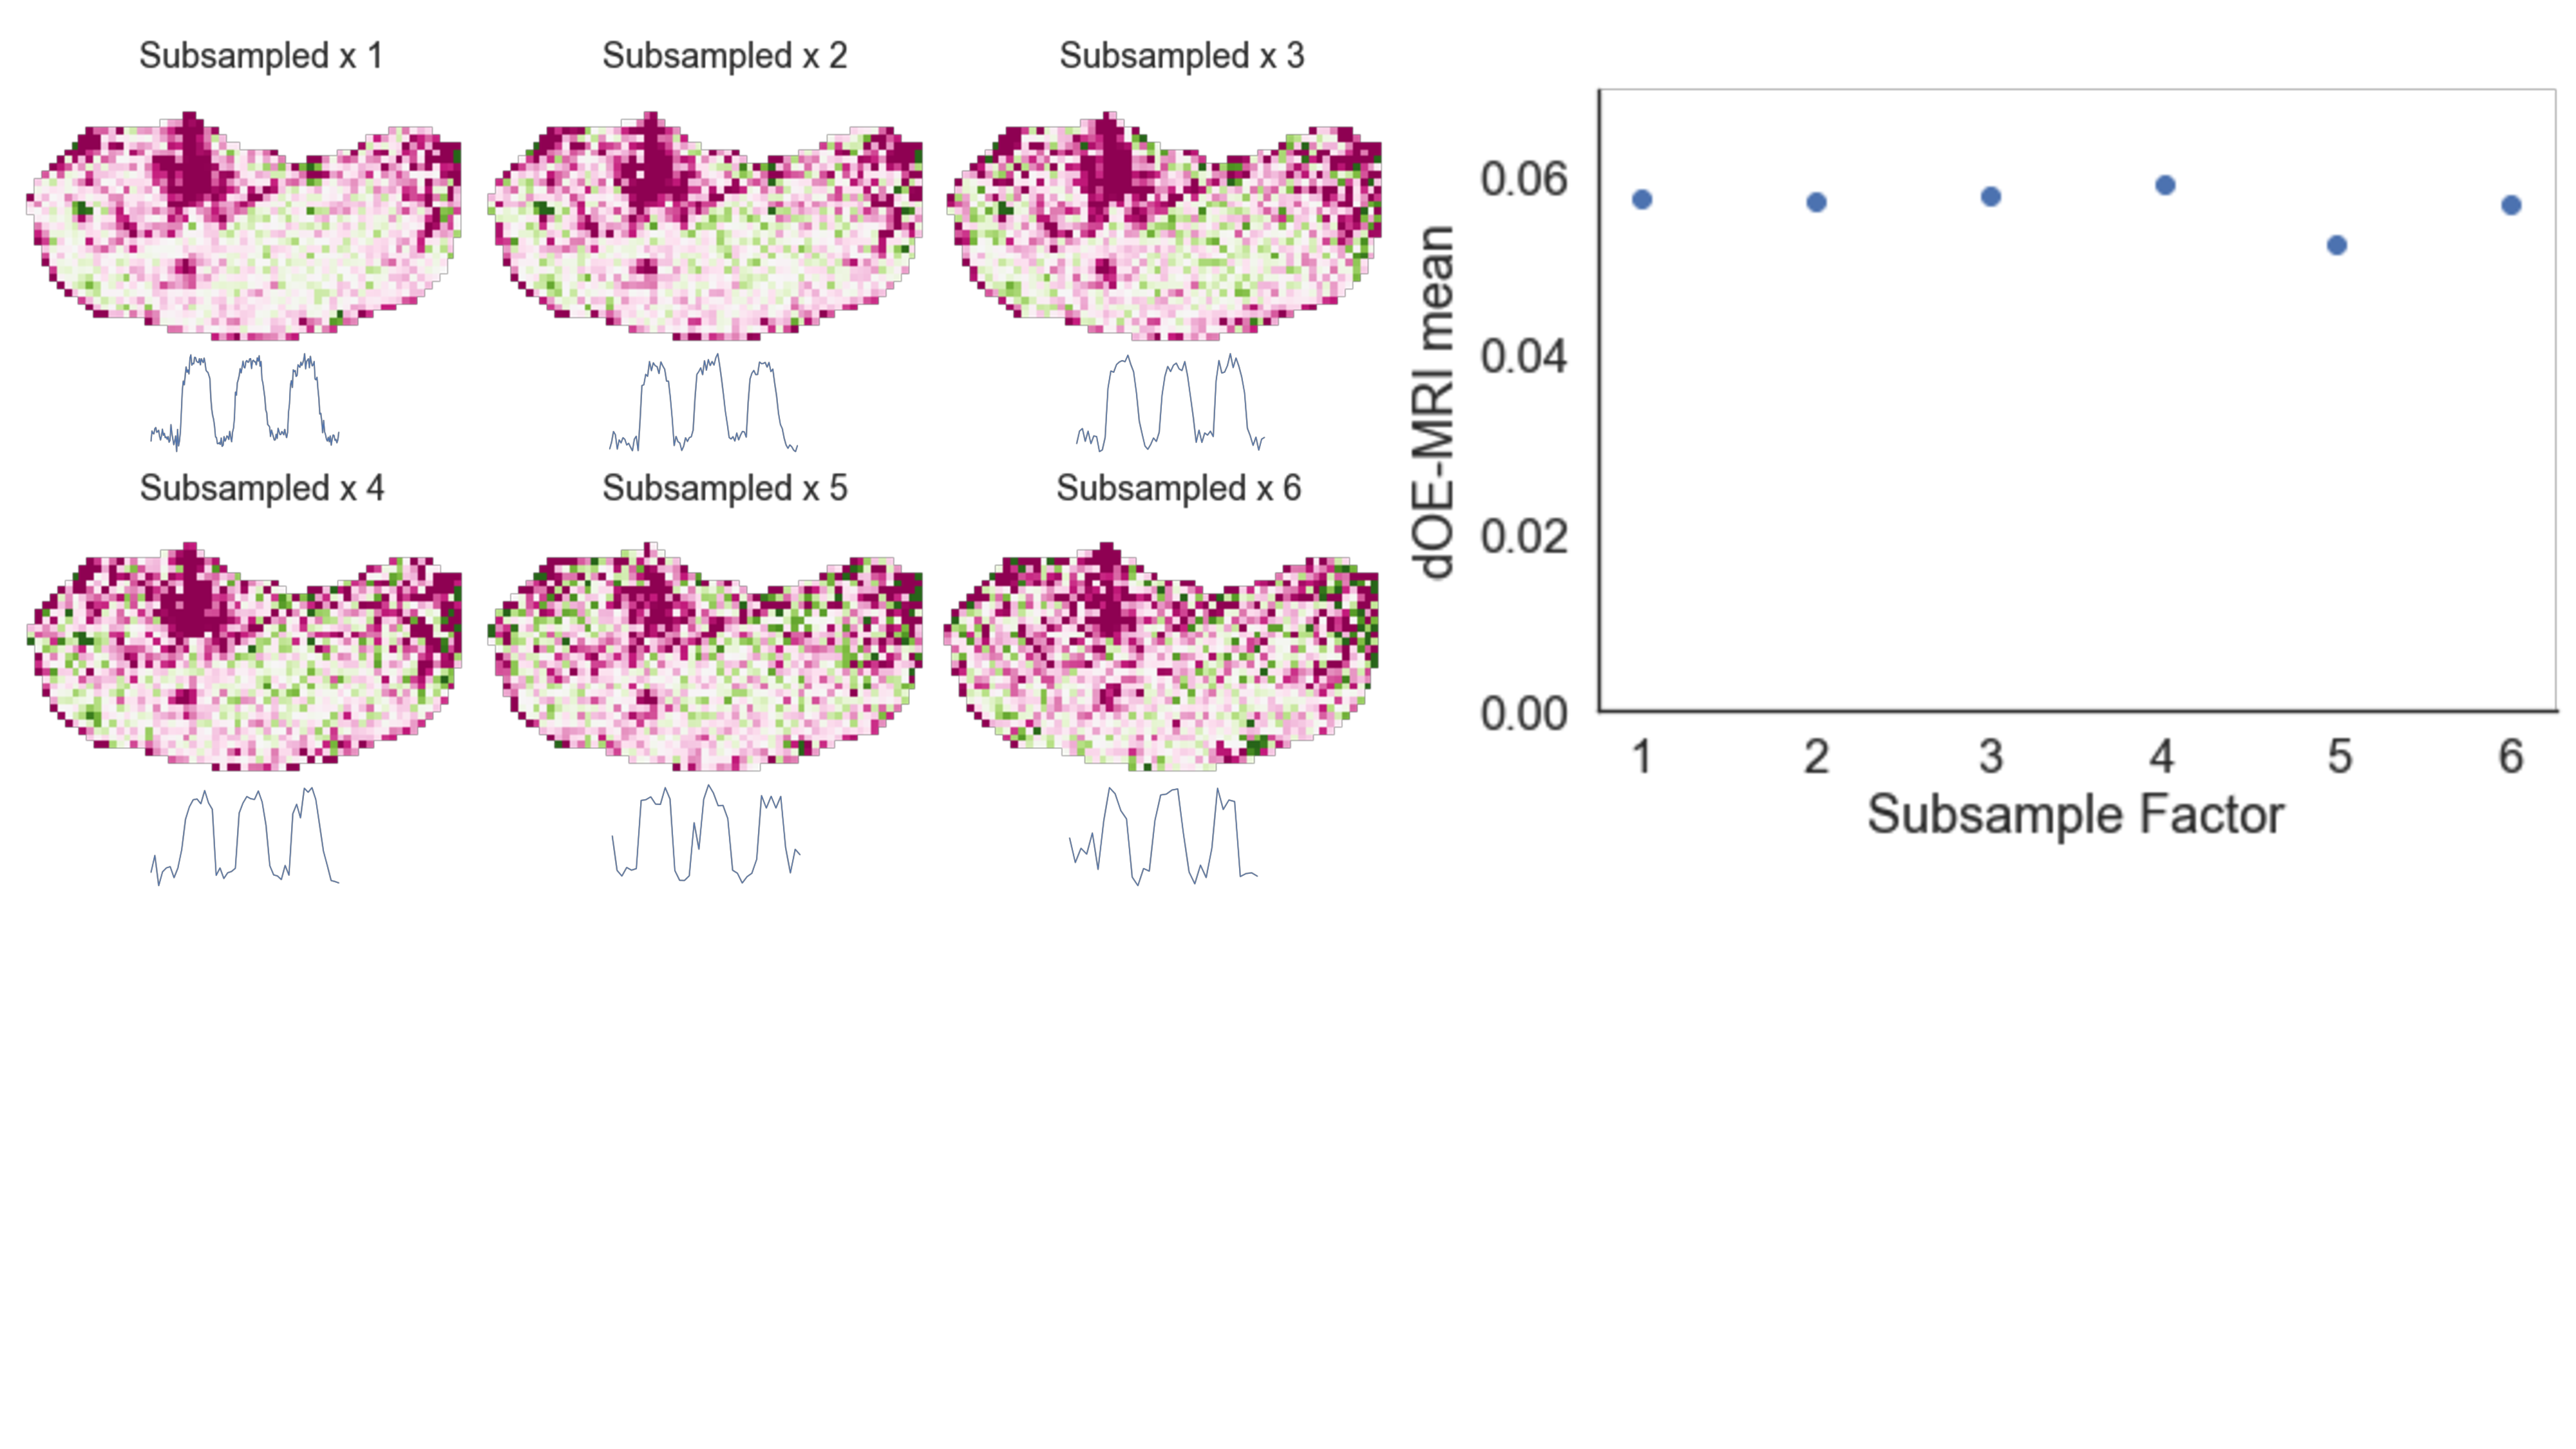
\includegraphics[width=\textwidth]{oemri_thesis1/oemri_thesis1-images/technical_subsample.pdf} % requires the graphicx package
   \caption{dOE-MRI maps and associated component traces of differently sampled data. To achieve different levels of subsampling, the raw data was spliced and then \acs{ICA} was applied. The oxygenation maps look very similar between different subsample factors. Temporal resolution and number of points were 4.3~s and 200 points (subsample 1), 8.5~s and 100 points (subsample 2), 12.8~s and 67 points (subsample 3), 17.1~s and 50 points (subsample 4), 21.3~s and 40 points (subsample 5), and 25.12~s and 34 points (subsample 6).}
   \label{subSample}
\end{figure}

\subsection{Exploring other independent components extracted using \acs{ICA}}

Figure~\ref{Sfig_components} shows the extracted independent components and their corresponding weighting factor maps for an application of \acs{ICA} on a OE-MRI scan.
Extracted components typically have a mix of high and low frequency responses and may include temperature drifts, breathing artefacts and other motion. 
For instance, c$_4$ is clearly the component of interest here as the cycling pattern is not present in any other component. 
We speculate that c$_1$ corresponds to a temperature drift over the course of the scan and c$_3$ is likely related to a breathing motion artefact. 
Component 2 is a relatively weak spurious signal fairly low in magnitude with no obvious spatial or temporal pattern. 
Additional physiological monitoring data is needed for a more thorough analysis of the other independent components and whether they can aid our understanding of the mechanism of action.

\begin{figure}[htbp]
   \centering
   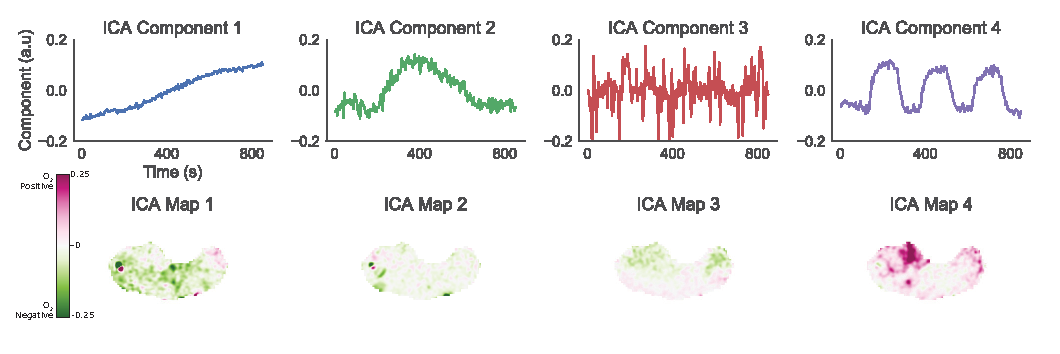
\includegraphics[width=\textwidth]{oemri_thesis1/oemri_thesis1-images/fig_components.pdf} % requires the graphicx package
   \caption{Plots of the four components extracted from \acs{ICA} are shown (($||c_i||=1, \forall i $) along with the corresponding  weighting factor maps (normalized to mean voxel wise mean signal intensity). Corrupting influences such as temperature drifts are often present and produce slowly increasing or decreasing trends (for e.g., $c_1$) and breathing artefacts corresponding to short-lived spikes ($c_3$). No explanation could be found for $c_2$.
No $c_1$
   \label{Sfig_components}}
\end{figure}

\subsection{Comparing oxygen responsiveness with \acs{dOE-MRI} across experiments}
\label{sec:correctionfactor}
It is necessary to characterize entire tumours in a compound fashion for comparison between groups or studies. 
Existing quantification methods have involved computing fractions of positively responding and negatively responding voxels as a surrogate for oxygen responsiveness in tumours with \acs{dOE-MRI}.
However, this semi-quantitative metric relies on a binary classification of voxels as either O$_2$ positive or O$_2$-negative.
Calculating fractions is sufficient to broadly categorize tumours as oxygenated or not but consequently, rich information about the level of response is lost.
Here we present an improved quantification method of \acs{dOE-MRI} data that captures the level of response and furthermore, allows direct comparison of data acquired at varying temporal resolutions.

Since each extracted \acs{ICA} component is scaled such that its norm is one ($||c_i||=1, \forall i $), weighting factor maps are only directly comparable between scans if \acs{dOE-MRI} images are acquired at the same sampling frequency over the duration of the cycling oxygen (14 minutes).
However, holding the sampling frequency fixed over different experiments is not practical as imaging tumours of different sizes require modification of the field of view and consequently, temporal and spatial resolutions.
A scaling $s$ factor must be applied to scale component map values so they can be compared between scans of different temporal resolutions,

\begin{equation}
s = \frac{\sqrt{N_{ref}}}{\sqrt{N}}
\label{correctionfactor}
\end{equation}

A reference sampling frequency should be chosen and in this study, it was chosen to be 0.24s$^{-1}$ (corresponding to N=198 images over the cycling oxygen).

Gas delivered to mice switches between room air and 100\% oxygen in two minute cycles, for a total of 14 minutes.
\acs{ICA} extracts the tissue response to the delivered oxygen, and four periods of room air interspersed with three periods of oxygen can be modelled mathematically using a general Heaviside function:

\begin{equation}
y(t) =
  \begin{cases}
                                   +b & \text{if $t\geq \frac{4T}{7}$} \\
                                   -b & \text{if $t< \frac{4T}{7}$} \\
  \end{cases},
\end{equation}

where $T$ is the total imaging time and $T/7$ is the time for a single segment of the gas challenge.
The Fast \acs{ICA} algorithm places a condition on the norm of the extracted component $y(t)$,

\begin{equation}
\sqrt{\sum_{i=1}^{N} \Bigl|y(t_i)\Bigr|^2} = 1.
\end{equation}

Simplifying the expression above for our $y(t)$ (the Heaviside function), we have:
\begin{align}
1 = \sqrt{b^2 \sum_{i=1}^{N} 1^2} \nonumber \\
b = N^{-\frac{1}{2}}
\end{align}

With this, we can compute the scaling factor directly using b$_{ref}$ =198 repetitions as the reference:

\begin{align}
s = \frac{b_{N}}{b_{ref}} \nonumber \\
s = \frac{\sqrt{198}}{\sqrt{N}} 
\end{align}

This scaling factor was applied to all \acs{dOE-MRI} maps used in this study to retain information about the level of response to the supplied oxygen across scans with different sampling frequencies.

%======================================================================
\section{Discussion}
% ======================================================================

In this study, we presented an improved method for OE-MRI that employs two synergistic techniques to achieve higher speed and greater sensitivity.
First, a repeated gas challenge was used to probe tissue response by introducing an independent signal modulation unrelated to spurious contributions such as temperature drifts and motion.
A repeating gas challenge improved the detection sensitivity of small amplitude signal changes that are typical of oxygen-enhanced MRI.
Second, a repeating signal modulation enabled further improved sensitivity through the use of \acs{ICA}, a signal processing technique to isolate source signals - T$_1$W changes due solely to the cycling oxygen - without knowledge of the tissue response (Figure~\ref{technique}).
While it is possible to generate correlation maps of the oxygen cycling paradigm with T$_1$W signal changes that appear very similar to \acs{dOE-MRI} maps, an \emph{a-priori} assumption of a response function is required for this approach (Figure~\ref{fig_correlation}).
Furthermore, presupposing a particular oxygen response function biases the identification of responding O$_2$-positive voxels (Figure~\ref{fig_correlation}) underscoring the need for a model-free approach to extracting the oxygen-responding component.

The unambiguous match of the identified component with the periods of the gas cycles increases the confidence that the small T$_1$W signal changes result from increased oxygen dissolved in the plasma and interstitial tissue fluids.
Maps from other extracted components (Figure~\ref{Sfig_components}) exhibit spatial patterns that could provide clues to the signal sources but associating meaning to them is challenging and would require additional data.
For example, even moderate shifts in temperature could drive a measurable change in T$_1$W signal during the timecourse, and a physiological monitoring system that is temporally synchronized to the MR acquisition could illuminate this confounding variable. 
Nevertheless, we have established reliability of the technique by comparing maps from each cycle of the gas challenge to the map incorporating data from all three oxygen-cycles and have found no significant differences.
In fact, the strong correlations between \acs{dOE-MRI} maps from each of the individual cycles of the gas challenge (Figure~\ref{fig_repeatability}) show that it is feasible to assess tissue oxygenation within 6 minutes.
Performing this analysis again with three-fold (Figure~\ref{fig_repeatability}) and six-fold (Section~\ref{sec:interleave}) temporally under-sampled data suggests that there is sufficient \acs{SNR} to successfully extract the oxygen responsive component  with even a subset of the data.

dOE-MRI offers a versatile technique where the duration of the cycles and gas challenge, temporal resolution and desired signal-to-noise can be modified based on the imaging objectives, which could include investigating intermittent perfusion or intervention-mediated changes in the tumour microenvironment. 
Of note, supplying excess oxygen to hypoxic tumour cells over time has the potential for increasing the baseline oxygen concentration, effectively reducing the hypoxic fraction and altering the tumour microenvironment~\cite{Linnik:2013hf}.
This would result in voxels becoming more oxygen responsive over progressive oxygen cycles and would depend on the tumour characteristics as well as the duration of the oxygen challenge.
This was not observed on the time scales in our study when using \acs{ICA} to extract changes in T$_1$W signal intensity just due to the gas challenge. 
Should it arise in other contexts it could possibly be mitigated by extending the air-breathing part of the cycle, or by extracting that as a separate component using \acs{ICA}.
The potential for creating a hyperoxia steady state by modulating oxygen duration is discussed further by Losert et al.~\cite{Losert:2002gt}.

Depending on the application of \acs{dOE-MRI}, quantitative O$_2$-positive and O$_2$-negative fractions can be obtained from \acs{dOE-MRI} maps as shown in this study, by deploying group \acs{ICA} techniques~\cite{Calhoun:2009jr}, or setting significance thresholds using a t-test~\cite{Greicius:2004ck} and computing z-scores~\cite{McKeown:1998wd}.
In a promising study, White et al.\ has shown that OE-MRI may be very relevant in developing prognostic factors to predict tumour response to hypofractionation by stratifying tumours that may benefit from oxygen breathing during irradiation~\cite{White:2016fz}.
Featherstone et al.\ have recently explored pre-clinical datasets using feature-extraction and clustering analysis and this may prove fruitful in understanding the behavior of subregions within a tumour microenvironment~\cite{Featherstone:2018cn}.
Future work to evaluate the utility of \acs{dOE-MRI} will ultimately depend on its context-dependent validation as a relevant measure of tumour hypoxia to dynamically characterize the clinically relevant oxygen status of tumours, relating this information to treatment sensitivities and outcomes.

% ======================================================================
\section{Conclusions}
% ======================================================================
In this study we extend existing oxygen-enhanced MRI techniques by adding a cycling element to the respiratory challenge and using a blind-source separation signal processing technique (\acs{ICA}) to extract the oxygen responsive component and responding voxels.
In the following chapters, we advance development and application of the technique and further refine it. 
In chapter~\ref{ch:oemri2} we attempt to validate \acs{dOE-MRI} measurements \emph{in vivo} using pimonidazole, a histological tumour hypoxia marker.
To further explore the oxygen dynamics in tumours we also characterized the oxygen replenishment curve as originally proposed by Losert et al.\ in the brain~\cite{Losert:2002gt}.
In chapter~\ref{ch:oemri3} we deploy the technique to assess tumour oxygenation changes following treatment with bevacizumab, an antiangiogenic agent.

\endinput

%% The following is a directive for TeXShop to indicate the main file
%%!TEX root = ../diss.tex

\chapter{Validation of oxygen-enhanced MRI in animals}
\label{ch:oemri2}

% ======================================================================
\section{Introduction}
% ======================================================================

Recently our group has proposed a new technique,\ac{dOE-MRI} to assess tumour oxygenation in vivo using MRI~\cite{Moosvi:2018ca}.
In this chapter we first extend the technique to characterize the extracted oxygen enhancing component used in \ac{DCE-US} experiments.
This model is then fit to the extracted \ac{ICA} components to assess the feasibility of using the fit parameters as biomarkers of oxygen response.
Finally we validate the method in tumour xenografts and compare \ac{dOE-MRI} maps to slice-matched histological sections.

\subsection{Theory: Modelling oxygen response}
\label{sec:lognormalfitting_theory}
A vascular network is a collection of multiple vessels including large arteries feeding smaller arterioles that ultimately deliver oxygen and nutrients to tissue via capillaries.
This complex vascular tree is modelled by assuming a fractal branching geometry with the distribution of vessel sizes and flow rates given by a lognormal velocity distribution~\cite{Qian:2000ca}:

\begin{equation}
P(v)=\frac{1}{\sigma_{f} \sqrt{2 \pi}} \cdot \frac{1}{v} \cdot \exp \left(-\frac{1}{2}\left(\frac{\ln (v)-u_{f}}{\sigma_{f}}\right)^{2}\right)
\end{equation}

Where $P(v)$ is the probability density function of the velocity $v$, $\mu_f$ and $\sigma_f$ are the mean and standard deviation of the distribution for the normally distributed random variable $ln(v)$.
The mean and standard deviation of a lognormal distribution are known quantities,

\begin{equation}
\operatorname{Mean}(v)=\exp \left(\mu_{f}+\frac{\sigma_{f}^{2}}{2}\right)
\end{equation}

\begin{equation}
\operatorname{Var}(v)=\exp \left(2 \mu_{f}+\sigma_{f}^{2}\right)\cdot \left(\exp \left(\sigma_{f}^{2}\right)-1\right)
\end{equation}

\begin{figure}[htbp]
   \centering
   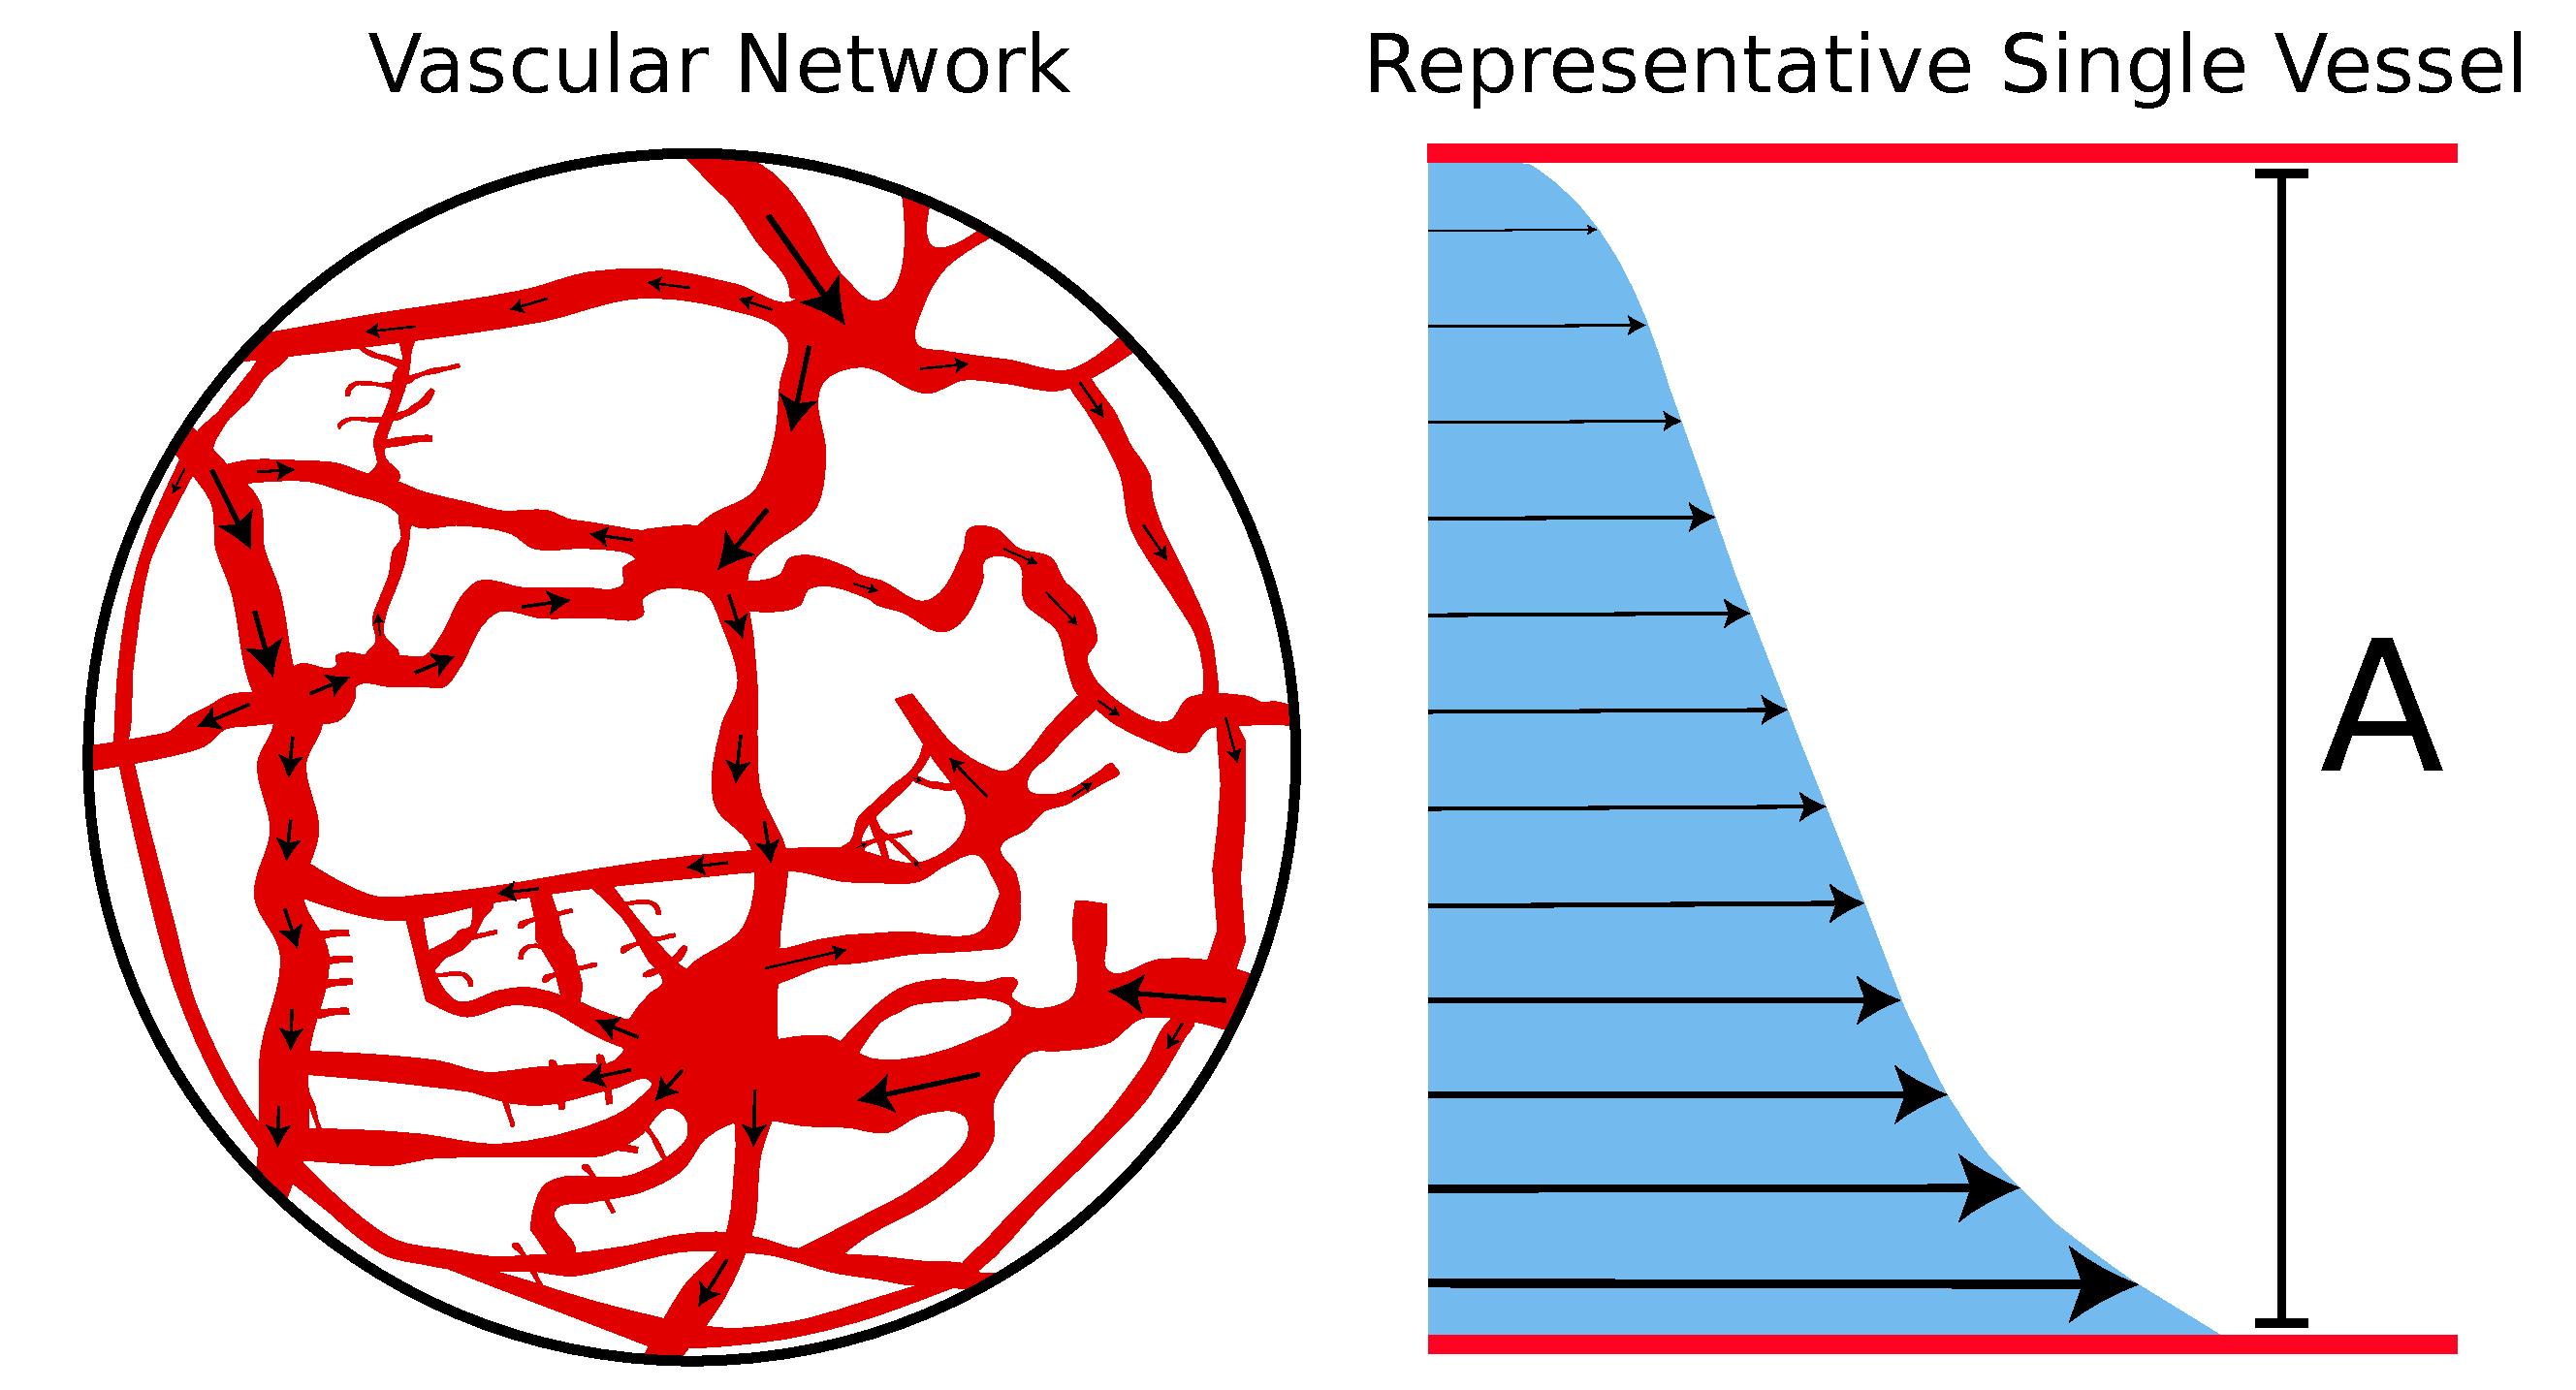
\includegraphics[width=\textwidth]{oemri_thesis2/oemri_thesis2-images/tumourVasculature.pdf} % requires the graphicx package
   \caption{Schematic representation of the complex vascular network (left) with multiple velocity profiles (arrows) and its equivalent representation as a single vessel with a distribution of flow profiles (right). The distribution of velocity profiles of the representative single vessel is the lognormal distribution. Schematic representation re-created from Hudson et al.~\cite{Hudson:2009jv}.}
   \label{lognormal}
\end{figure}

Figure~\ref{lognormal} shows a schematic of the vascular network modelled as a representative single vessel with a lognormal distribution of velocity profiles.
Therefore the flow function for a vascular network is given by,

\begin{equation}
F(z, t)=\frac{A}{2} \cdot \operatorname{erfc}\left(\frac{\ln (z / t)-u_{f}}{\sigma_{f} \sqrt{2}}\right)
\end{equation}

Where A is defined as the total vascular area, z represents the spatial displacement of oxygen through the blood stream, $\mu_f$ is the mean velocity and $\sigma_f$ is the standard deviation of the velocity distributions. 
The velocity $v$ was transformed for convenience to $z/t$ to facilitate integration over the slice thickness $z$.

This lognormal flow profile model has been used to describe the replenishment of microbubbles injected into the blood stream in \ac{DCE-US}~\cite{Hudson:2009jv}.
The generalized representation of the replenishment time-intensity signal requires two components: an ultrasound beam-specific profile that is weighted in the z-direction due to a non-uniform slice profile and the flow profile. 
The expression is,

\begin{equation}
S(t) = \int_{V} B(x,y,z) \cdot F(x,y,z,t) \cdot dV
\end{equation}

where $B(x,y,z) = 1$ in MRI because of relatively uniform slice profiles. 
Integrating over the imaging plane ($x,y$) and assuming a slice thickness of 1mm ($z$), the final model for fitting \ac{dOE-MRI} data becomes,

\begin{equation}
S(t)= \left[\frac{A}{2}\left(z \operatorname{erfc}\left(\frac{\ln \left(z/t\right)-\mu_f}{\sqrt{2} \sigma_f}\right)-t e^{\sigma_f^{2} / 2+\mu_f} \operatorname{erf}\left(\frac{\sigma_f^{2}+\mu_f-\log \left(z/t\right)}{\sqrt{2} \sigma_f}\right)\right)\right]_{z=0}^{z=1mm}
\label{lognormalFitEquation}
\end{equation}

Where A is defined as the total vascular area, $\mu_f$ is the mean velocity and $\sigma_f$ is the standard deviation of the velocity distributions. 

% ======================================================================
\section{Methods}
% ======================================================================
\subsection{Animals}
Female NRG (NOD rag gamma) mice were implanted with murine squamous cell carcinoma (SCCVII; 5x10$^5$ cells in 50 $\mu$l serum-free media; cells provided by Dr.\ J. Evans) in the dorsal subcutaneous region.
All mice were injected with 60 mg/kg pimonidazole hydrochloride (HypoxyProbe) 30-min prior to imaging to label hypoxic cells and were euthanized within 15-min of imaging completion.
Mice were anesthetized with isoflurane using 1.5-2.0\% isoflurane for the duration of MR imaging sessions until euthanasia, and were positioned supine on the custom surface coil apparatus.
Throughout the imaging session, a small animal monitoring system (SAII Instruments, Stony Brook, NY, USA) was used to monitor respiration rate, varying between 80-100 breaths per minute, and body temperature, maintained at 36.8 $\pm$ 0.5$^\circ$C using a continuous airflow heater. 
Tumours were embedded and frozen in optimum cutting temperature medium (OCT; Tissue-TEK) with their largest diameter 8-10 mm.
All animal experimental procedures were carried out in compliance with the guidelines of the Canadian Council for Animal Care and were approved by the institutional Animal Care Committee.

\subsection{Immunohistochemistry}
Co-planar MRI slices and histological sections were obtained by imaging perpendicular to the longest tumour axis in MRI and serial-step 10 $\mu m$ cryosections were cut at 0.5-mm intervals in the same plane.
Slides were then fixed in acetone-methanol for 10-min and whole sections were immunohistochemically stained~\cite{Kalra:2017is} for \ac{CD31} (visualized using secondaries labeled with Alexa 647nm) to label blood vessels, and for pimonidazole (HypoxyProbe-1; visualized using secondary labeled with Alexa 546nm) to label hypoxic cells. 
Sections were then stained using Hoechst 33342 (bisbenzimide) to label all cell nuclei.
Whole-tumour sections were imaged using a robotic fluorescence microscope (Zeiss Axioimager Z1), a cooled, monochrome CCD camera (Retiga 4000R; QImaging), a motorized slide loader and x-y stage (Ludl Electronic Products) and customized ImageJ software~\cite{Collins:2007jr}. 
Adjacent microscope fields of view were tiled such that images of entire tumour cryosections were captured at a resolution of 1.5 $\mu m$/pixel. 
Using anatomical landmarks and accumulated thicknesses of serial-step sections as estimates of distances from the edges of whole tumours, sections were chosen to match the MR slices. 
ImageJ and user-supplied algorithms were used to super impose digital images which were then manually cropped to tumour tissue boundaries with staining artifacts removed. 
A threshold was applied to images to identify positive pimonidazole staining, and the number of positive pixels was determined as a percentage of the total number of pixels in the tumour image. 
Overlaid greyscale images were converted to false colour for visualization with pimonidazole as green and \ac{CD31} as magenta.

\subsection{MR Imaging}
As previously described in Section~\ref{doemri_mrianalysis1}.

\subsection{\ac{dOE-MRI} Analysis}

As previously described in Section~\ref{doemri_mrianalysis2}.

\subsection{Model Fitting}
\label{sec:lognormalfitting_methods}
Equation~\ref{lognormalFitEquation} was fit to the first 100 seconds of the \ac{ICA} component trace after oxygen was first delivered to the mouse. 
Model fitting was done with the \texttt{LMFIT} package~\cite{Newville:2019jt} using the Levenberg-Marquardt method.
A free fit parameter was added corresponding to a vertical offset to account for the \ac{ICA} component starting below 0. 
For each fit, three parameters describe the shape of the oxygen response: A (vascular area), $\mu_f$ (mean velocity) and $\sigma_f$ (standard deviation) of the velocity distributions.
A sample fit using equation~\ref{lognormalFitEquation} is shown in figure~\ref{fig:lognormal_sample}.

\begin{figure}[htbp]
   \centering
   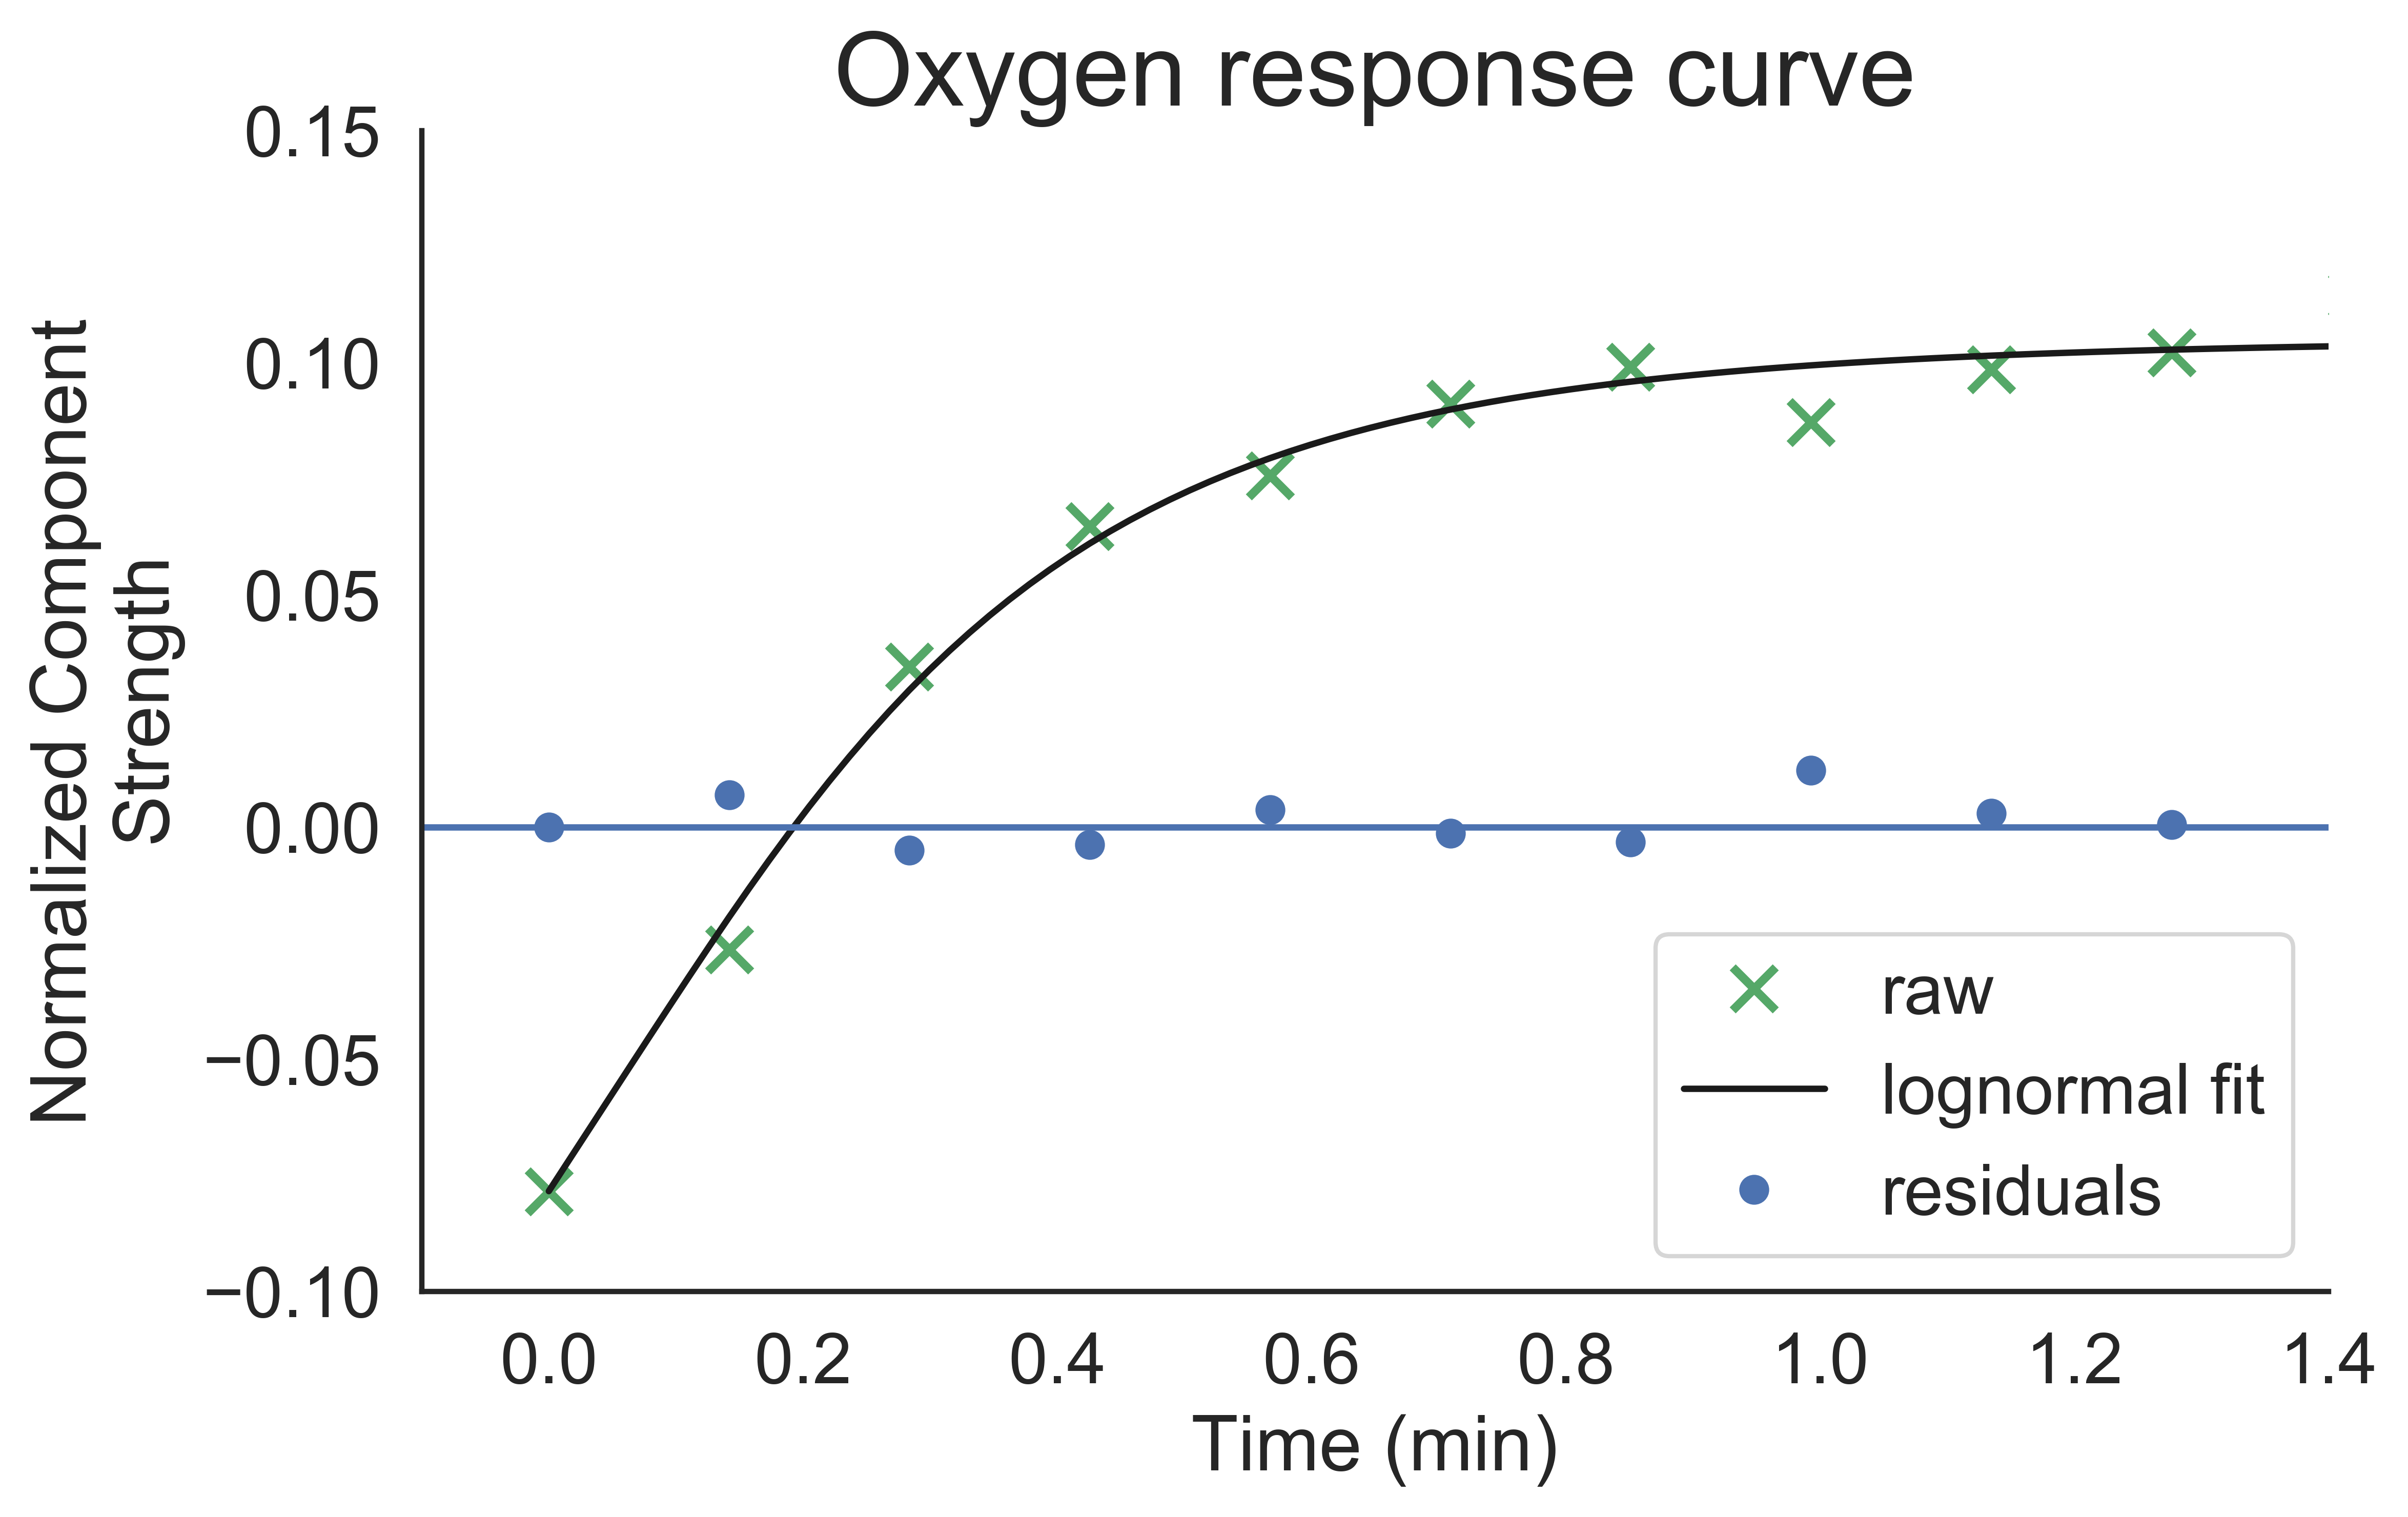
\includegraphics[width=\textwidth]{oemri_thesis2/oemri_thesis2-images/technical_SampleFit.png} % requires the graphicx package
   \caption{Fit of equation~\ref{lognormalFitEquation} to an oxygen response curve with the residuals plotted along the x-axis for each point.
   For this fit, $A= 0.18$, $v_f = 0.66 mm/s$, and $\sigma_f = 0.58 mm/s$.}
   \label{fig:lognormal_sample}
\end{figure}

% ======================================================================
\section{Results}
% ======================================================================
%%%%%%%%%%%%%%%%% ############ BEGIN *versatile* section from paper 1 ############ 
\subsection{ICA enabled \ac{dOE-MRI} detects variable oxygenation in a range of tumour models}
\label{sec:rangeModels}
Tumours of human and murine origin and comprising a variety of tumour microenvironments were imaged, including fast growing, highly vascularized murine squamous cell (SCCVII) and human ovarian carcinomas (SKOV3), slower growing and well vascularized human breast cancer (BT-474), as well as a relatively fast growing but more poorly vascularized human colon colorectal carcinoma (HCT-116).
The inter-model heterogeneity of the tumours is reflected in the mean fraction of negative voxels in the \ac{dOE-MRI} maps, which were 46 $\pm$ 6\% for BT-474, 36$\pm$3\% for HCT-116, 31$\pm$5\% for SCCVII, and 14$\pm$4\% for SKOV3 tumours. 
Considerable intra-tumour heterogeneity is also observed within some models, particularly the BT474.
\ac{dOE-MRI} maps representing the mean fraction of negative voxels are shown for each tumour type in Figure~\ref{versatile}.
\begin{figure}[htbp]
   \centering
   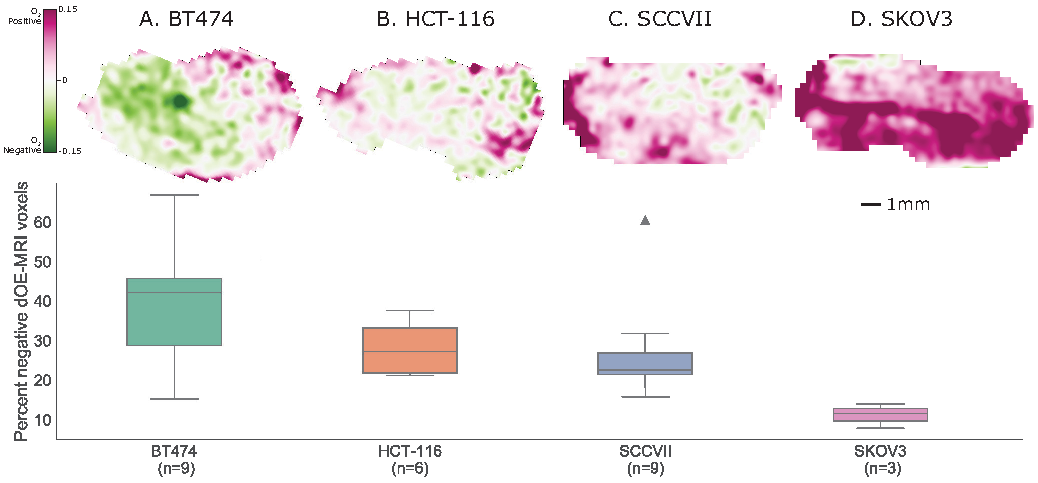
\includegraphics[width=\textwidth]{oemri_thesis1/oemri_thesis1-images/fig2_versatile.pdf} % requires the graphicx package
   \caption{Top: \ac{dOE-MRI} maps for four tumour models HCT-116, BT-474, SCCVII, and SKOV3 are shown. Chosen slices are representative of the mean percent negative \ac{dOE-MRI} fraction for the respective tumour model.
Bottom: The box-whisker plot shows the quartiles of percent negative \ac{dOE-MRI} voxels for all imaged tumours.
\label{versatile}}
\end{figure}
%%%%%%%%%%%%%%%%% ############ END *versatile* section from paper 1########### 

%%%%%%%%%%%%%%%%% ############ BEGIN section about fitting ############

\subsection{Vascular area $A$ and mean velocity $v_f$ do not vary across tumour models, but $\sigma_f$ differentiates between tumours}
\label{sec:lognormalfitting_results}
% Analysis notebook: 
% http://localhost:8889/user/fmoosvi/notebooks/OxygenMRI/Thesis%20Exploring/OEMRI%20chapter%202%20-%20lognormal%20fitting%20aggregations.ipynb
Equation~\ref{lognormalFitEquation} was fit to the oxygen response kinetics for three tumour models (SCCVII, HCT-116, and BT474).
Figure~\ref{fig:lognormal_CHB} shows the raw data and the fit for each animal. 
Group averages for each of the three parameters $A$, $v_f$ and $\sigma_f$ are shown in box plots.
The parameter $\sigma_f$ discriminated between tumour types in this analysis and $\sigma_f$ for SCCVII tumours ($\sigma_f$ = 0.30 $\pm$ 0.09 mm/s) was statistically significantly lower than the HCT-116 tumours ($\sigma_f$ = 0.52 $\pm$ 0.12 mm/s; p = 0.047) as well as the BT474 tumours ($\sigma_f$ = 0.76 $\pm$ 0.19 mm/s; p = 0.044).
The effect size for both comparisons was quite small: Hedge's g = 0.05 for SCCVII vs. HCT-116 tumours and $g$ = 0.02 for SCCVII vs. BT474. 
No significant difference was found when comparing $\sigma_f$ of HCT-116 and BT474 tumours.
High intratumour variability was present in all tumours, but particularly in the BT474 tumour models.
The SKOV3 tumours were not considered as part of this analysis due to low sample size (N=3). 

\begin{figure}[htbp]
   \centering
   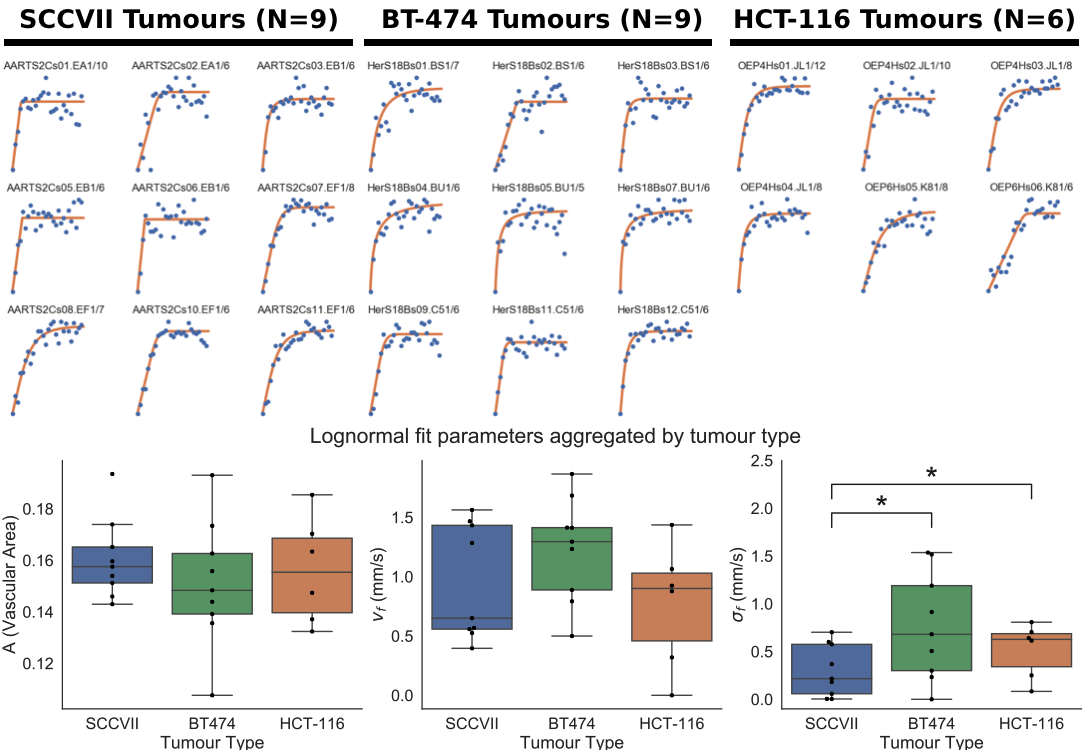
\includegraphics[width=\textwidth]{oemri_thesis2/oemri_thesis2-images/lognormalFittingAgg_CHB.png} % requires the graphicx package
   \caption{Top: Individual fits to the oxygen response curve for each animal and tumour type.
   Bottom: Box plots showing the median value and quartiles for $A$, $v_f$, and $\sigma_f$ across the three tumour models.}
   \label{fig:lognormal_CHB}
\end{figure}
%%%%%%%%%%%%%%%%% ############ END section about fitting ############ 

%%%%%%%%%%%%%%%%% ############ BEGIN *histo validation* section from paper 1 ############ 

\subsection{\ac{dOE-MRI} maps correspond to matched histology sections}
\label{sec:histoSections}
Tumour tissue cryosections obtained to match MR imaging slices were stained for vasculature (\ac{CD31}) and regions of pimonidazole-labeled hypoxia and are compared side-by-side; Figures~\ref{fig_sccvii} and~\ref{fig_hct116} provide five examples for each of SCCVII and HCT-116 tumour models for detailed review.
Generally, in corresponding \ac{dOE-MRI} maps for both tumour models O$_2$-positive voxels align with the most oxygenated regions of histology sections, where pimonidazole labeling is absent, however many areas of mismatch are also observed. 
More consistent is that O$_2$-positive voxels do not typically correspond to tissues identified as hypoxic in the histology sections (i.e. labeled with pimonidazole).
In general, the more necrotic HCT-116 tumours have fewer oxygenated (O$_2$-positive) regions and significantly more hypoxic (O$_2$-negative) regions in the \ac{dOE-MRI} maps, compared to the SCCVII tumours that have no necrosis. 
Pimonidazole labeling is heterogeneously dispersed within regions of viable tissue containing tumour blood vessels for both SCCVII tumours, Figure~\ref{fig_sccvii}, and HCT-116 tumours, which typically have greater amounts of necrosis, Figure~\ref{fig_hct116}.
Figure~\ref{histo_correlations} shows the fraction of negative \ac{dOE-MRI} voxels correlated with the histological hypoxic fraction. 
For SCCVII tumours (n=9) there was an excellent correlation, with Pearson's r = 0.91 (\textit{p}=0.0016). 
However the correlation in the HCT-116 tumours (n=6) was poor, with r=0.13 (\textit{p}=0.81). 

\begin{figure}[htbp]
   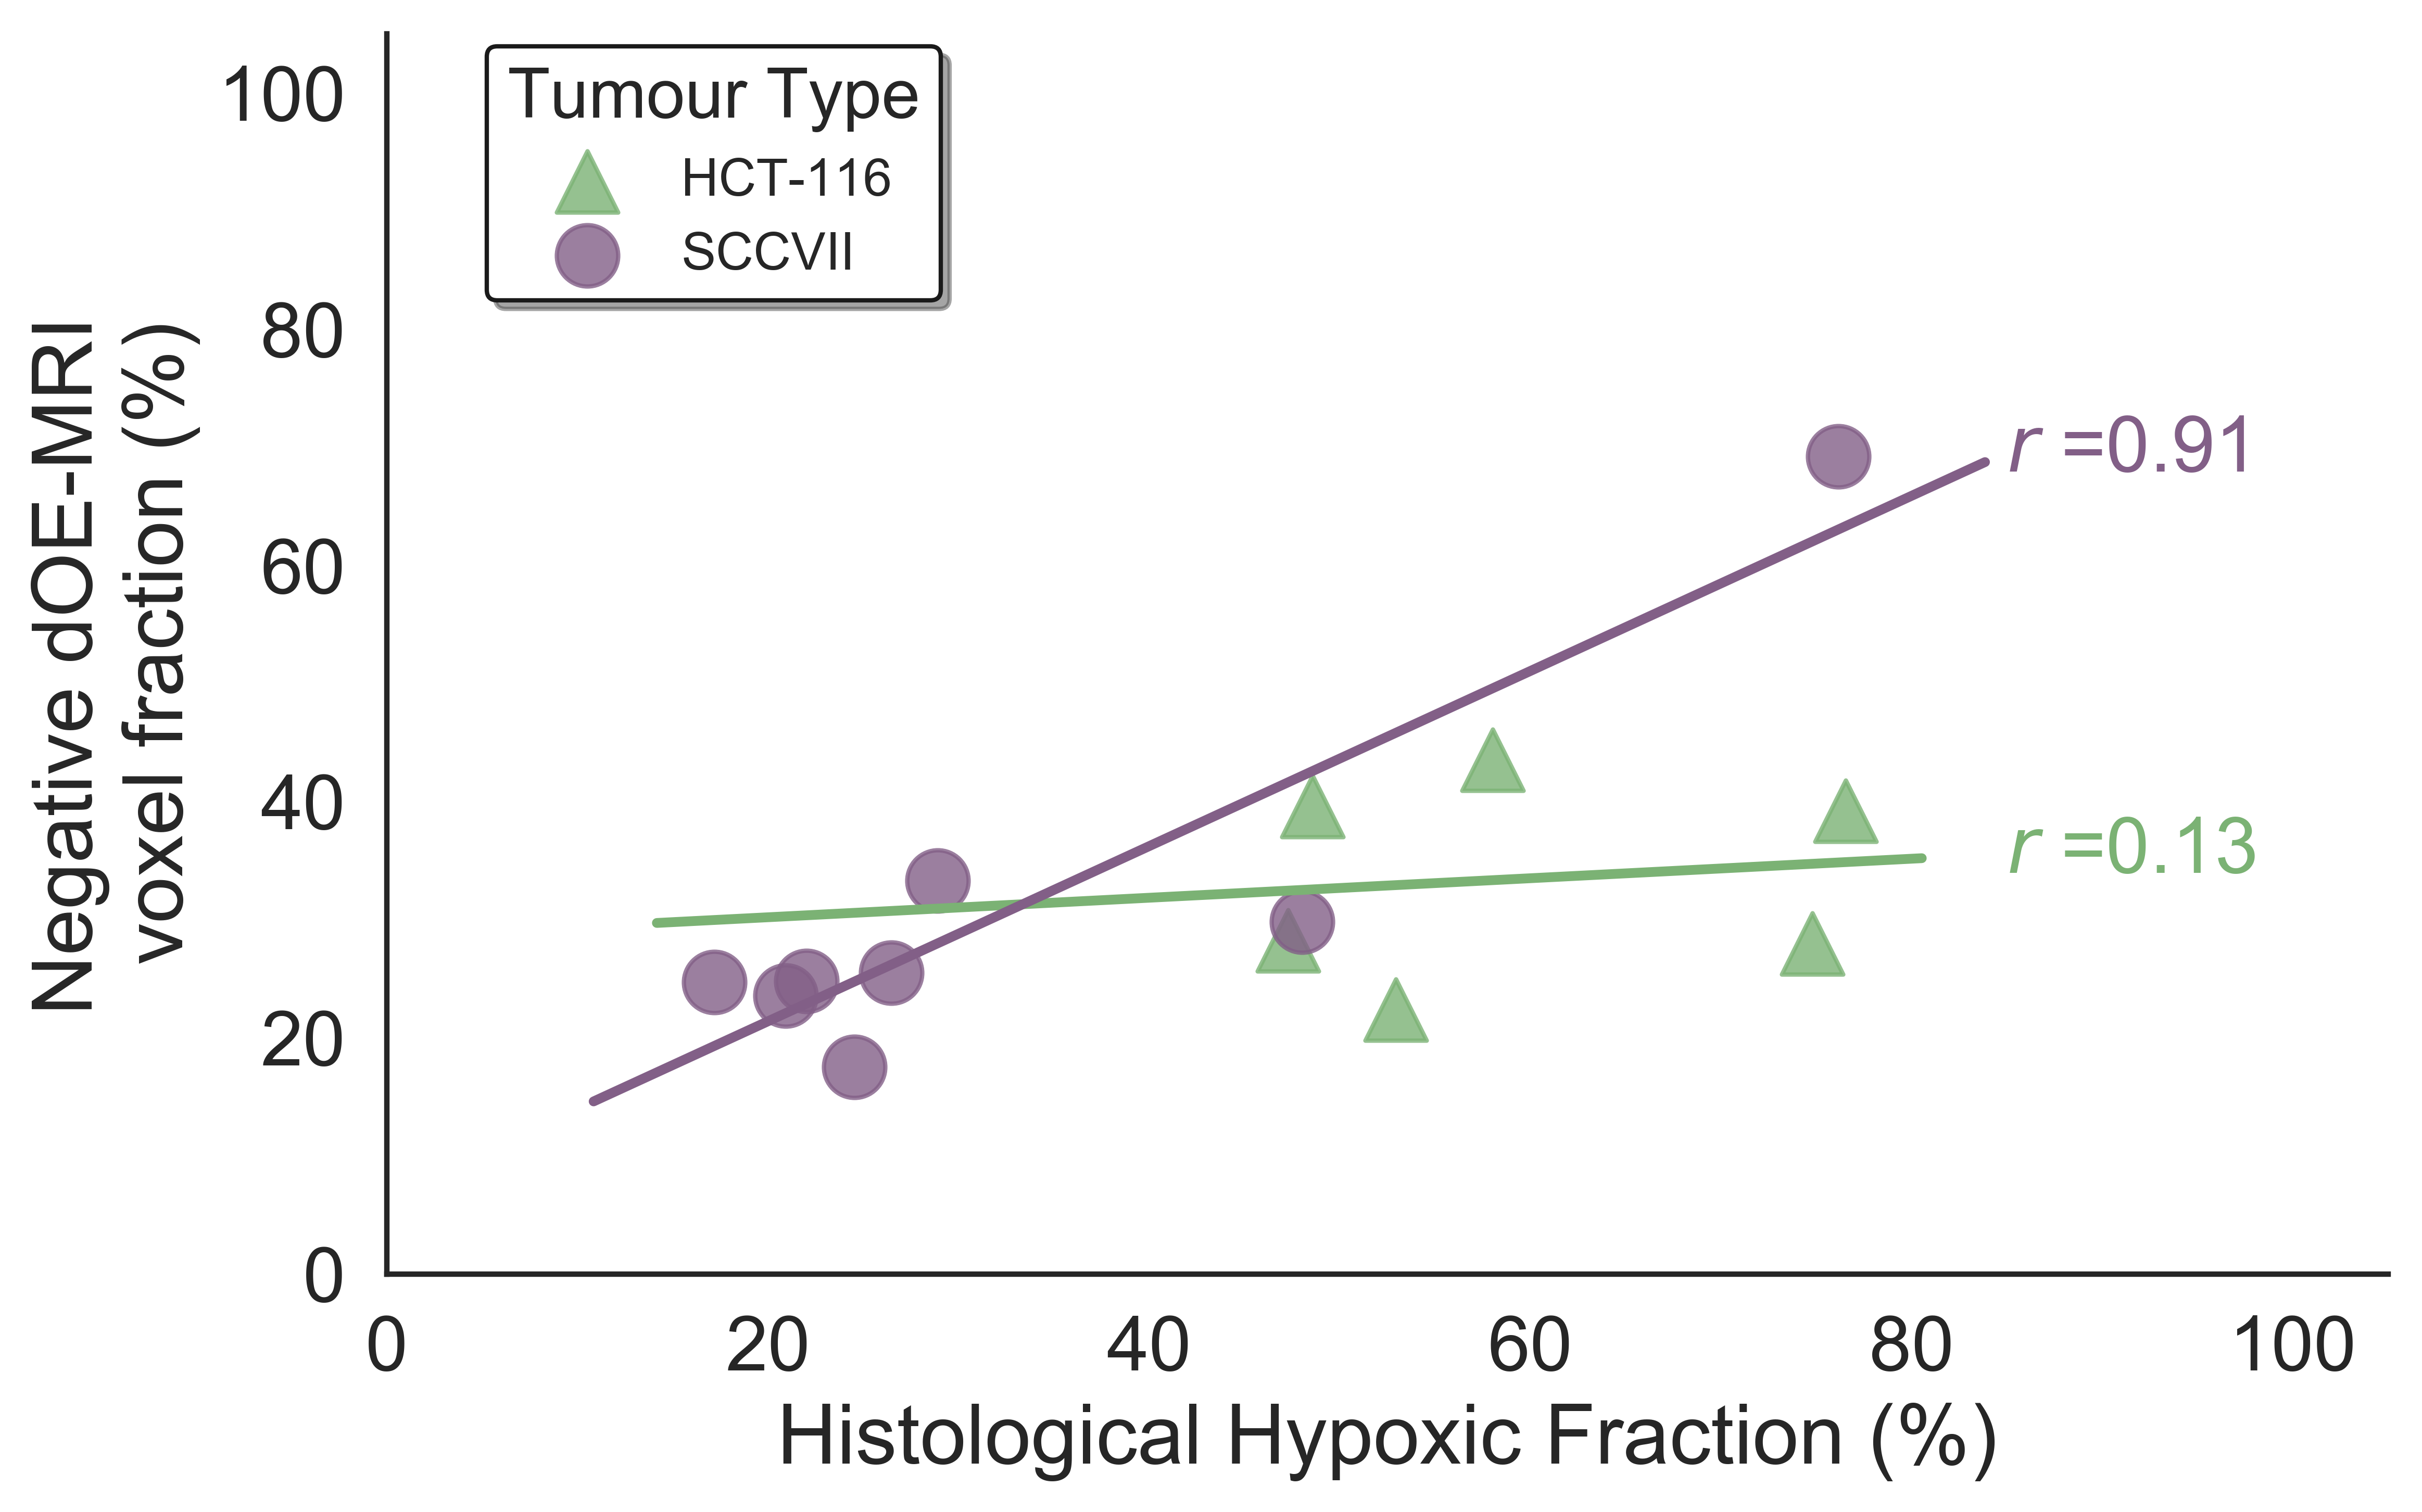
\includegraphics[width=\textwidth]{oemri_thesis1/oemri_thesis1-images/histocorrel2.png} % requires the graphicx package % note for Firas: I changed the aspect ratio of this figure slightly
   \caption{The proportion of negative \ac{dOE-MRI} voxels is plotted against the histological hypoxic fractions with Pearson's r = 0.91 for SCCVII tumours and r = 0.13 for HCT-116 tumours.
   \label{histo_correlations}}
\end{figure}

\begin{figure}[htbp]
   \centering
   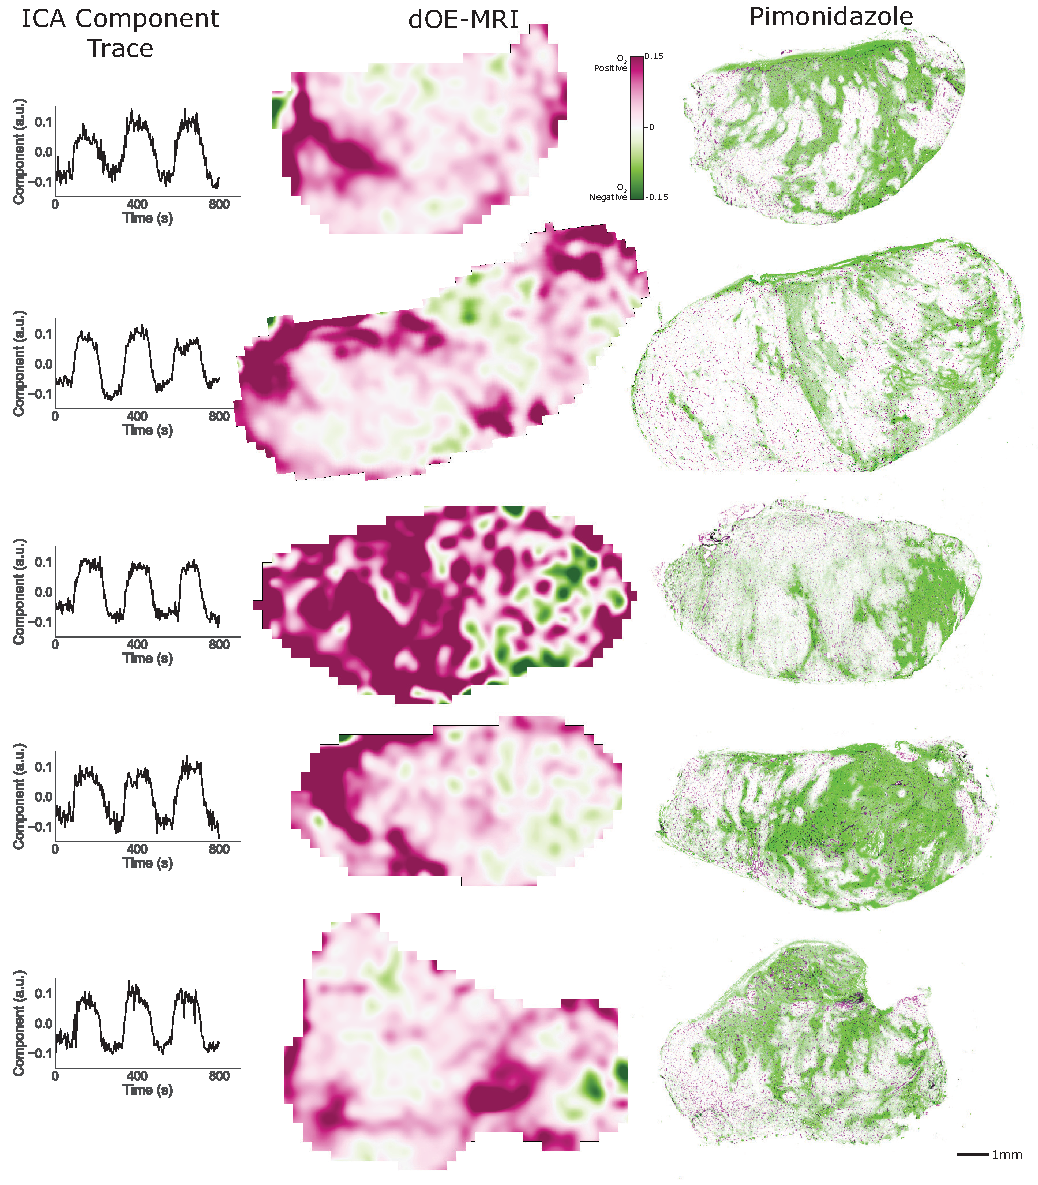
\includegraphics[width=0.9\textwidth]{oemri_thesis1/oemri_thesis1-images/fig6_sccvii.pdf} % requires the graphicx package
   \caption{SCCVII murine tumours with slice-matched histological images depicting pimonidazole-labeled hypoxia (green) and \ac{CD31}-stained vasculature (purple) are shown next to the \ac{dOE-MRI} parameter maps similarly colored with O$_2$-positive (purple) and O$_2$-negative (green) areas. Corresponding \ac{ICA} extracted components are also shown.
   \label{fig_sccvii}}
\end{figure}
\begin{figure}[htbp]
   \centering
   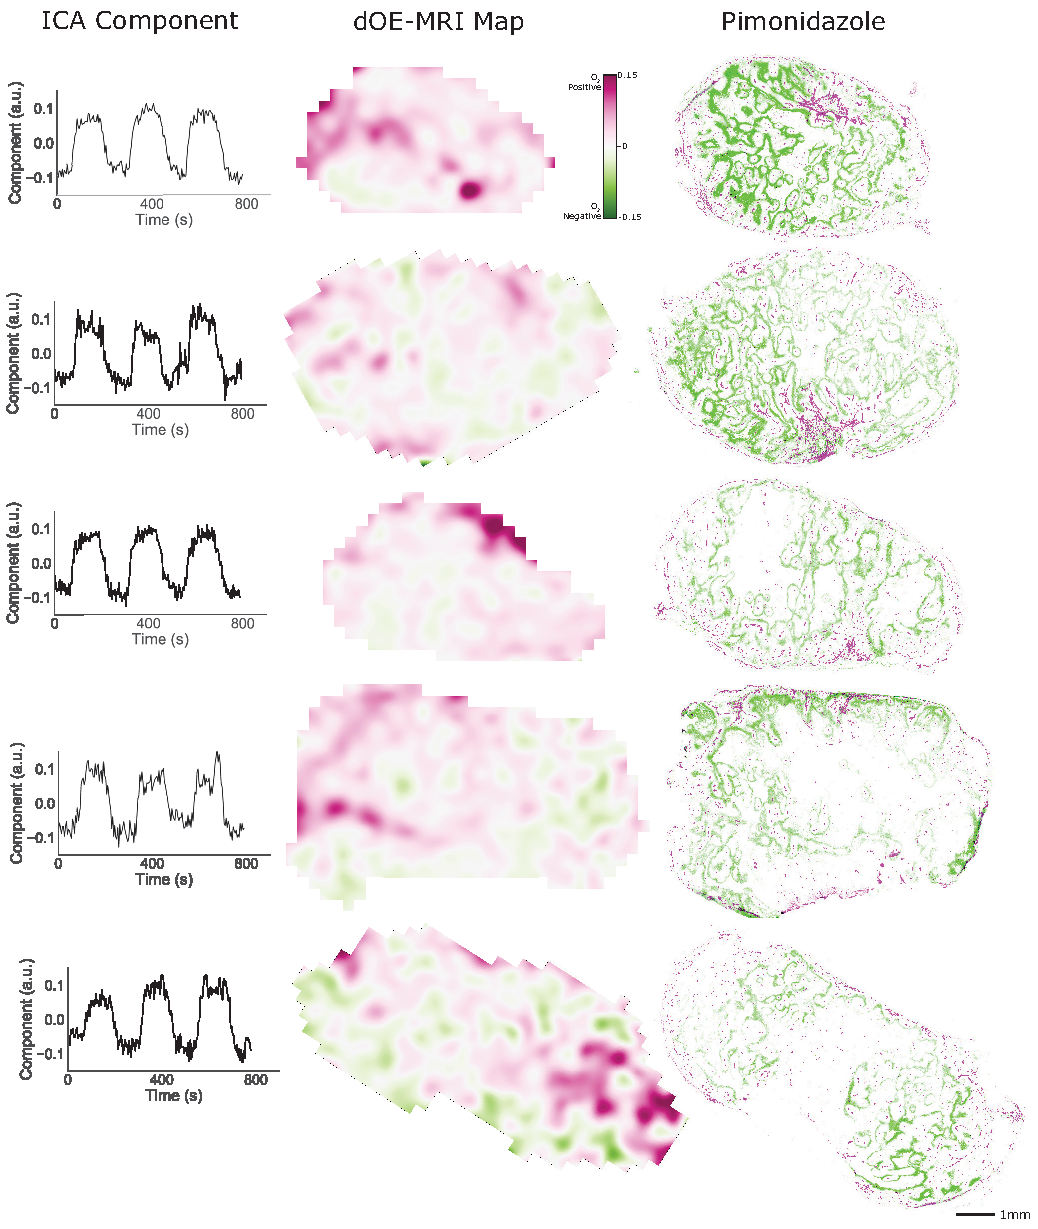
\includegraphics[width=0.9\textwidth]{oemri_thesis1/oemri_thesis1-images/fig7_hct116.pdf} % requires the graphicx package
   \caption{HCT-116 human colorectal xenografts with slice-matched histological images depicting pimonidazole-labeled hypoxia (green) and \ac{CD31}-stained vasculature (purple) are shown next to the \ac{dOE-MRI} parameter maps similarly colored with O$_2$-positive (purple) and O$_2$-negative (green) areas. Corresponding \ac{ICA} extracted components are also shown.
   \label{fig_hct116}}
\end{figure}

%%%%%%%%%%%%%%%%% ############ END *histo validation* section from paper 1########### 

% ======================================================================
\section{Discussion}
% ======================================================================

The improved sensitivity of our \ac{dOE-MRI} technique results in broader applicability of \ac{dOE-MRI}, as we found that an oxygen-enhancing component was extracted successfully in all imaged animals across a range of tumour models and environments (Figure~\ref{versatile}).
In this study we also modelled the oxygen response curves in the tumour vasculature by deploying models developed in \ac{DCE-US} and adapting them for \ac{dOE-MRI}.
Fitting equation~\ref{lognormalFitEquation} to the oxygen response curves results in three physiologically relevant parameters.
Unsurprisingly, the vascular area $A$ and the mean velocity $v_f$ do not appear to be vary between the three tumour models studied(Figure~\ref{fig:lognormal_CHB}).
The third parameter $\sigma_f$ is the standard deviation of the velocity distribution and is related to the structural organization and morphology of the vascular network~\cite{Hudson:2009jv}.
Thus, we hypothesized that the oxygen response curves and in particular, $\sigma_f$ may capture information about the vascular organization in different tumour models.
The SCCVII tumour is a very aggressive and fast growing tumour~\cite{Khurana:2001wb}, which implies a chaotic vascular network with a low degree of fractality (propensity to branch in a fractal pattern with large arteries branching to smaller arterioles, leading to extremely small capillaries).
This behaviour would result in a narrow range of vessel sizes and velocity profiles in our lognormal velocity profile,  and manifests in a low $\sigma_f$ value for SCCVII tumours relative to the other tumour lines.
While only $\sigma_f$ appears to be useful in delineating tumour models, $v_f$ and $A$ may be useful metrics to quantify the oxygen response curves of tumours after drug interventions. 
  
A limitation of OE-MRI is the difficulty in interpreting areas that do not show a reduction in T$_1$ as they may be either dead tissues that are \textit{unperfused and not oxygenated} or living, viable tissues that are \textit{perfused but not oxygenated} due to poor oxygen content of the supplying vessels. 
The latter population are of greater interest to the oncology community as it is these hypoxic but viable cells that have significant influence on treatment outcomes~\cite{Horsman:2016go}. 
The \ac{dOE-MRI} technique presented here successfully correlates tumour oxygenation \ac{dOE-MRI} and histology measures in SCCVII tumours but, despite improvements to sensitivity, a similar quantitative comparison in the HCT-116 tumour line showed poorer association (Fig.~\ref{histo_correlations}). 
This is likely attributable to the much higher amounts of necrosis typical of the HCT-116 model relative to SCCVII (Figs.~\ref{fig_sccvii} and \ref{fig_hct116}).
Mitigations to this limitation have been explored elsewhere and generally require a perfusion mask or $T_2^*$ - either technique can be added to the OE-MRI method proposed here to exclude necrosis and further improve sensitivity of the technique.

Application of existing OE-MRI techniques across a range of tumour models with varying perfusion characteristics has yielded mixed success without masking for perfused tissue.
For instance, O'Connor reported that in the highly perfused 786-0-R tumour lines, 85-96\% of all imaged tumour voxels were deemed to be oxygen-enhancing~\cite{OConnor:2016ee}.
In those tumours, there was a good correlation between histological hypoxic fraction and oxygen refractory voxels.
However, in the more weakly perfused SW620 tumours where only 76\% of the voxels are oxygen-enhancing, there were no significant correlations with the histological hypoxic fraction.
These issues were resolved by combining OE-MRI with DCE-MRI as a perfusion mask to select only perfused voxels for oxygenation assessment, thereby distinguishing between the viable hypoxic environment and necrotic dead tissues and improving the specificity and sensitivity of OE-MRI data. Using an IAUGC$_{60}$ map from DCE-MRI as a mask to obtain Oxy-R fractions O'Connor et al. showed good correlation with the histological hypoxic fraction~\cite{OConnor:2016ee}.
In more recent work, Little et al. showed oxygen enhancement in tumours with a histological hypoxic fraction as high as 43\%~\cite{Little:2018iu} and this translated very well to a study of six renal cell carcinoma patients.
Linnik et al. reported excellent correlation between percentage of ``negative AUC$_{OE}$'' ($O_2$-negative) voxels and percentage of hypoxic areas in the highly vascular preclinical U87MG tumour xenografts~\cite{Linnik:2013hf}.
A second approach for differentiating between viable but hypoxic regions and unperfused dead tissues, is to combine OE-MRI with $T_2^*$W acquisition and the BOLD effect to classify regions~\cite{Little:2018iu,Zhao:2015ez,White:2016fz,Burrell:2013je,Yang:2018vo} that show both effects. 
Excess oxygen in the blood will induce changes in Hb saturation, which alter the T2* resulting in a robust measure of areas with functioning vasculature. 
Conceivably, the saved acquisition time achieved with under-sampling T$_1$W \ac{dOE-MRI} suggests that $T_2^*$W images could also be acquired to concurrently assess the blood oxygen level dependent (BOLD) response. 

Within the relatively short 14-minute imaging time, both the HCT-116 and SCCVII tumours show only minor changes in the oxygenation maps between cycles (Figure~\ref{fig_correlation}).
In longer imaging sessions, or during administration of an intervention, these same tumours may exhibit varying oxygenation patterns between cycles.
Periods of oxygen-starvation and re-oxygenation in tumours have been termed intermittent hypoxia and can arise due to temporary vessel occlusions~\cite{Dewhirst:2009de,Bayer:2011js}.
Recent work on measuring intermittent hypoxia in patients using R$_2^*$~\cite{Panek:2017ge} shows that interest in this phenomenon continues but the importance of intermittent hypoxia in tumours is unclear largely due to poor availability of techniques to measure it in the clinic~\cite{Michiels:2016hv}.
The relatively short imaging time for \ac{dOE-MRI} makes assessing temporal oxygenation changes possible within a timescale on the order of minutes by comparing correlation maps generated from sequential cycles.

Typically, histological validation of MR data is done by collapsing rich histology data into a single metric, such as a hypoxic fraction, with whole-tumour or single-slice average comparisons.
While this is sometimes a useful validation approach, it may not reflect the highly heterogeneous patterns of hypoxia that are known to vary spatially and temporally, even within the same tumour, as well as between tumour types as highlighted in Figures~\ref{histo_correlations}-\ref{fig_hct116}. 
Further complications are encountered with respect to validation of tools to assess hypoxia considering that hypoxia is not simply a binary metric. Instead, tumour oxygenation exists as a spectrum beginning with some tissues that may be normoxic, at levels similar to neighbouring normal tissues of origin, and can continue decreasing through levels of hypoxia to near anoxia where cells are still viable but are no longer able to proliferate.
Eventually cells die in the absence of oxygen, and when this occurs in large numbers there can be significant regions of necrosis in solid tumours. 
A range of oxygenation levels are likely to be present in the highly heterogeneous microenvironments of all solid tumours, but what is of interest to the oncology community is \emph{clinically relevant} hypoxia~\cite{Horsman:2012kw}.
This refers to measurable tumour oxygenation levels that are biomarkers of physiologically meaningful phenomena, including patient prognosis or tumour sensitivity to treatments, such as immunotherapy or radiotherapy. The relevant oxygenation status for any biomarker of interest may include levels spanning from moderate to severely hypoxic. 
Pimonidazole has been demonstrated as a clinically relevant marker of hypoxia, but poor or inconsistent correlation with pimonidazole, as we have seen in our imaged tumours, does not exclude other measures of tumour oxygenation from potential utility.

Measurable pimonidazole-adduct formation occurs when the O$_2$ tension in the vicinity drops below 10 mmHg~\cite{Gross:1995wq} but in \ac{dOE-MRI}, O$_2$-positive voxels are extracted as excess oxygen dissolves in the plasma and interstitial tissue fluid to decrease T$_1$.
Voxels where T$_1$ has significantly increased has previously been correlated to poorly perfused regions and likely corresponds to hypoxic regions where the excess oxygen is picked up by deoxyhemoglobin molecules~\cite{Linnik:2013hf,Burrell:2013je,Remmele:2012df}.
The exact mechanism for a T$_1$ increase as a result of oxygen inhalation has not yet been confirmed~\cite{Zhao:2015ez,Linnik:2013hf}, however, based on careful work of Silvennonin et al., characterizing behavior of T$_1$ in fresh bovine blood~\cite{Silvennoinen:2003gn}, we speculate the corresponding T$_1$W signal decrease may arise due to the conversion of deoxyhemoglobin to hemoglobin in the perfused vessels of hypoxic regions .
O$_2$-positive regions in \ac{dOE-MRI} maps are generally in good agreement with well perfused areas of histology images for both HCT-116 and SCCVII tumours, as shown in Figures~\ref{fig_sccvii} and~\ref{fig_hct116}.
Voxels exhibiting signal reduction with the O$_2$ stimulus in \ac{dOE-MRI} maps (O$_2$-negative, green) typically correspond with histology (pimonidazole, green) but not all pimonidazole-labeled regions appear as O$_2$-negative voxels.
Similarly, \ac{CD31}-stained tumour regions are not exclusively O$_2$-positive in the \ac{dOE-MRI} maps because not all tumour vessels are perfused.
In fact many perfused blood vessels are only intermittently perfused and consequently, the measurement of hypoxia is time-sensitive.
Mismatches between \ac{dOE-MRI} and histology may be attributed in part to the different sensitivities and detection thresholds for measuring hypoxia and oxygenation in the \ac{dOE-MRI} and histology-based modalities, as well as potential mismatch between the timing of pimonidazole-labeling and \ac{dOE-MRI} data acquisition. 

%\subsection{random snippets}
%O$_2$ positive or O$_2$-negative fractions are immune to this phenomenon, information about the level of response can be retained simply by applying the scaling factor when comparing scans at different temporal resolutions
% ======================================================================
\section{Conclusions}
% ======================================================================

In this chapter, we have validated the \ac{dOE-MRI} technique by comparing oxygenation maps with pimonidazole stained histology images. 
The versatility of the technique was apparent due to its applicability in multiple tumour models; though, the presence of large necrotic areas in tumours poses some challenges when comparing oxygenation status with pimonidazole staining.
We have also shown that the lognormal velocity profile model from \ac{DCE-US} is applicable to oxygen response curves obtained from \ac{ICA} and \ac{dOE-MRI} and the parameter $\sigma_f$ is useful in quantifying the vascular morphology of tumours.
\ac{dOE-MRI} assesses tumour oxygenation fairly reliably \emph{in vivo} and the next application is to see whether the technique is sensitive to oxygenation changes brought on by chemotherapies.

% ======================================================================
 %\section{References}
% ======================================================================
%\bibliography{oemri2}

%\bibliographystyle{vancouver-authoryear}

%\end{document}
%% The following is a directive for TeXShop to indicate the main file
%%!TEX root = ../diss.tex

\chapter{Applications of oxygen-enhanced MRI}
\label{ch:oemri3}

\section{Preface}

A new term has been introduced in this chapter to compare what has previously been referred to as ``dOE-MRI values''.
The normalized component weighting factor value is now shortened to be \acs{NCWF}.

% ======================================================================
\section{Introduction}
% ======================================================================

Dynamic oxygen-enhanced MRI (\ac{dOE-MRI}) has recently been proposed by our group to assess tumour oxygenation in vivo using MRI~\cite{Moosvi:2018ca}. 
This technique measures T$_1$-weighted changes in tissues in response to a cycling oxygen challenge, with the responsive signals detected using \ac{ICA}. 
Briefly, oxygenation can be assessed \emph{in vivo} by administering a simple gas challenge (switching between two-minute periods of medical air and 100\% O$_2$) during the \ac{dOE-MRI} scan and then using \ac{ICA} to extract the tissue response.
\ac{ICA} is a blind-source separation algorithm that separates multiple signal sources by maximizing statistical independence of individual components~\cite{Hyvarinen:2000vk}.
Various flavours of oxygen-enhanced MRI (OE-MRI) have been proposed but all essentially leverage the paramagnetic properties of inhaled oxygen.
White et al.\ have shown that OE-MRI may be very relevant in developing prognostic factors to predict tumour response to hypofractionation by stratifying tumours that may benefit from oxygen breathing during irradiation~\cite{White:2016fz}.
In this study, we apply \ac{dOE-MRI} to mice bearing tumour xenografts to assess the effect of a common antiangiogenic agent.
We hypothesized that \ac{dOE-MRI} with group-\ac{ICA} can detect \ac{VEGF} ablation-induced changes to oxygenation of SCCVII tumours 48 hours following treatment.

\subsection{VEGF inhibition and bevacizumab}

\acs{VEGF} is a key regulator of angiogenesis as the \acs{VEGF} molecule is rate-limiting in normal and pathological growth of blood vessels.
Bevacizumab is a monocolonal antibody that binds \acs{VEGF} and inhibits growth of blood vessels~\cite{Ferrara:2004fa} and inhibits tumour growth.
It is marketed for clinical use under the name Avastin$^{\tiny{\textrm{\textcopyright}}}$ (Genentech Inc., California, USA) on tumours and its effects and outcomes have been widely reported~\cite{Keating:2014gt, Pavlidis:2013bj, Barnett:2013bt, Kumler:2014gb}.
Tumour xenografts receiving monocolonal antibodies to VEGF have consistently shown reductions in quantitative perfusion parameters from a variety of non-invasive imaging modalities including \acs{DCE-US}~\cite{Wang:2015bb}, \acs{DCE-MRI}~\cite{OConnor:2009cg}, and micro PET~\cite{Nagengast:2007hx}.
For \ac{DCE-US}, Wang et al.\ reported a significant reduction in peak enhancement, area under the curve, relative blood volume, and relative blood flow just 24 hours after a treatment of 10~mg/kg of bevacizumab~\cite{Wang:2015bb}.  
Several \ac{DCE-MRI} animal and human studies have shown reductions in \acs{K$^{trans}$}, \acs{$v_p$}, and \acs{$v_e$} after administration of antiangiogenic agents, including bevacizumab~\cite{Yang:2018hz}.
Tumour growth delay data also clearly indicates that growth is slowed after treatment with bevacizumab~\cite{Yang:2018hz} and other similar \acs{VEGF}-inhibitors~\cite{OConnor:2012ie}.

It is well established that after treatment with antiangiogenic agents, the normalized vasculature is characterized by a reduction in vessel permeability, tortuosity, greater coverage by pericytes and a more normal basement membrane~\cite{Jain:2005gk}. 
These morphological changes often result in functional changes as well including decreased interstitial fluid pressure, increased tumour oxygenation, and improved delivery of nutrients (and drugs)~\cite{Jain:2005gk}.
Bevacizumab is an expensive drug with many adverse effects~\cite{Keating:2014gt} so selective targeting of patients that are most likely to benefit from it should improve its cost-effectiveness~\cite{Barnett:2013bt}.
In this study, we present an exciting application of our non-invasive imaging-based technique with no requirement for an exogenous contrast agent to assess tumour oxygenation before and after treatment with bevacizumab.

% ======================================================================
\section{Methods}
% ======================================================================
\subsection{Animals}
Female NRG (NOD rag gamma) mice were implanted with murine squamous cell carcinoma (SCCVII; $5\times 10^5$ cells in 50~$\mu$l serum-free media; cells provided by Dr.\ J.\ Evans) in the dorsal subcutaneous region.
Tumours were imaged when their largest diameters reached approximately 8-10~mm.
All mice were injected with 60~mg/kg pimonidazole hydrochloride (HypoxyProbe) 30~min prior to imaging to label hypoxic cells and were euthanized within 15~min of imaging completion.
Mice were anesthetized with isoflurane using 1.5-2.0\% isoflurane for the duration of MR imaging sessions until euthanasia, and were positioned supine on the custom surface coil apparatus.
Throughout the imaging session, a small animal monitoring system (SA Instruments Inc., Stony Brook, NY, USA) was used to monitor respiration rate, varying between 80-100~breaths per minute, and body temperature, maintained at ${36.8\pm 0.5^\circ}$C using a continuous airflow heater. 
Tumours were embedded and frozen in optimum cutting temperature medium (OCT; Tissue-TEK).


\subsection{Immunohistochemistry}
As previously described in Section~\ref{doemri_histo}.

\subsection{MR Imaging}
As previously described in Section~\ref{doemri_mrianalysis1}.
All scans were acquired with the same spatial resolution and geometry and an experienced operator outlined the tumour on each slice of the RARE image to construct the region of interest (\acs{ROI}) for each animal and then transferred to all other scans.
Tumour volumes were measured by multiplying individual voxel volume ($0.3\times 0.3\times 0.1$~mm$^3$) and the count of total number of voxels included within the manually drawn \acs{ROI}.

% Imaging was performed using a 7T scanner (Bruker Biospec) with a transmit quadrature volume coil and a custom built surface receive coil. 
% An axial RARE image was acquired to localize the tumour (T$_E$/T$_R$=10.7/4250, RARE factor 8) and a T$_1$ map was acquired using the Look-Locker method. We acquired
% \acs{dOE-MRI} scans using a 2D multi-slice FLASH-based sequence for a total scan time of about 14~min.
% During the \ac{dOE-MRI} scan, breathing gas was alternated between medical air and 100\% oxygen every 2 minutes using a 3-channel gas mixer (CWE, Philadelphia, USA) for a total of 3 air-oxygen-air cycles.

\subsection{\ac{dOE-MRI} Analysis}

As previously described in Section~\ref{doemri_mrianalysis2}.
%%%%
% A suite of in-house software was developed using the python machine learning library scikit-learn~\cite{Pedregosa:2011tv}, specifically \texttt{sklearn.decomposition.FastICA} based on the technique described by Hyvarinen~\cite{Hyvarinen:2000vk}.
% The Fast\ac{ICA} algorithm is applied to serially acquired T$_1$W images and the output is a paired set of components and weighting factors for each voxel in the dataset.
% The deflation-based Fast\ac{ICA} (python package scikit.sklearn v0.17.1) was used to analyze the data. 
% Extracted independent components are not ordered and while the component selection can be automated, in this study an observer was assigned to select the appropriate component.
% The number of independent components for each imaging session was chosen by the operator and ranged from 4-9 to ensure the cyclic behaviour of the T$_1$W signal intensity corresponding to the gas challenge appeared in only one component. 
% The \ac{dOE-MRI} maps were obtained by dividing the \ac{ICA} weighting-factor maps by the mean signal-intensity maps to obtain a spatial map for the strength of a particular voxel's contribution to the component of interest.
Briefly, in these \ac{dOE-MRI} maps, voxels are coloured to indicate the amount by which a given pixel intensity time course is modulated by the oxygen-related component.
To compare \ac{dOE-MRI} maps between mice with different temporal resolutions, a scaling factor was applied as discussed previously (see section~\ref{sec:correctionfactor}).
Final normalized \ac{dOE-MRI} maps were obtained by dividing each pixel of the component map for each animal with the mean signal-intensity over time of the corresponding pixel in the \ac{dOE-MRI} scan. 
Mean normalized component weighting factor (\acs{NCWF}) are reported as a marker for tumour oxygenation with high values indicating increased oxygenation while negative values suggest decreased oxygenation or increased levels of hypoxia. 
Mann-Whitney U non-parametric tests are used to assess the difference between experimental groups and Hedge's $g$ was calculated to determine effect size when $p<0.05$.
%The green-white-purple colour spectrum depicts the degree to which voxels respond to the cycled gas challenge.
%Purple indicates O$_2$-positive voxels whose time course exhibits a higher and more positive contribution from the corresponding \ac{ICA} component, representing an increase in T$_1$W signal intensity in response to the supplied 100\% oxygen, and corresponding to areas with excess dissolved oxygen.
%O$_2$-negative voxels that show a decrease in T$_1$W signal intensity with a negative contribution from the corresponding \ac{ICA} component under 100\% oxygen breathing are depicted as green. 
%Regions whose T$_1$W signal intensity time courses responds only weakly or not at all to the gas challenge are shown in white hues.
%A feature of Fast\ac{ICA} is that the norm of each component is normalized to 1 ($||c_i||=1, \forall i$) and the corresponding weighting factor map carries the scaling factor.

\subsection{Experiment Summaries}
General methods common to both experiments have been described above, below are implementation details for each of the two separate experiments presented in this study.

\subsubsection{Experiment 1: Evaluating the utility of dOE-MRI to assess oxygenation improvements after anti-VEGF ablation therapy}
\label{sec:B20_expt1}
\noindent\textbf{Animals}: Seventeen (17) mice were implanted for this experiment with eight left untreated and nine mice treated with 5mg/kg mouse anti-VEGF antibody (B20-4.1.1, Genentech) 48 hours prior to imaging.

\noindent\textbf{MRI}: Axial \ac{dOE-MRI} scans were acquired with 90 repetitions using a 2D FLASH based sequence with T$_E$/T$_R$=2.67/133 ms, flip angle $\alpha$=40$^\circ$, 16 slices each 1mm thick, FOV of 3.84cm x 2.16 cm, encoding matrix of 128x72, and a temporal resolution of 9.6s for a total scan time of about 14 minutes.

\subsubsection{Experiment 2: Assessing oxygenation changes in intramuscular and subcutaneous tumours Anti-VEGF ablation therapy in \acs{IM} vs. \acs{SC} tumours}
\noindent\textbf{Animals}: Thirteen (13) mice were used in this experiment. 
3 mice were implanted with SCCVII in the dorsal subcutaneous (SC) region.
10 mice were implanted in both the dorsal subcutaneous (SC) as well as in the hind limb intramuscular (IM) region.
To account for the accelerated rate of growth for tumours implanted intramuscularly, one-fifth of the cells were implanted \acs{IM} (1x10$^5$ cells in 50$\mu$l serum-free media).
Separate ROIs were drawn on the T$_2$W images to outline both the \acs{SC} and \acs{IM} tumours.
5 mice were treated with 5mg/kg B20 24 hours prior to imaging and 8 were untreated controls.

\noindent\textbf{MRI}: Coronal images were acquired to enable simultaneous imaging of both tumours in the same field of view.
All \ac{dOE-MRI} scans were acquired using a 2D FLASH based sequence with TE = 2.67~ms, spatial resolution $0.3\times 0.3\times 1$~mm$^3$ and flip angle $\alpha=40^\circ$.
To accommodate additional slices and image both tumours in the same scan while maintaining spatial resolution, not all imaging parameters in the \ac{dOE-MRI} scan could be fixed. 
Table~\ref{scanparams} summarizes the key differences in the acquisition parameters for all \ac{dOE-MRI} sequences used in experiment 2.

\begin{table}[]
\centering
\begin{tabular}{c|c|c|c|c|c}
Experiment & Mice & TR/ms & Slices & Repetitions & Temporal resolution (ms)\\
\hline
 1 & 17& 133 & 16 & 90  & 9.6  \\
 2 & 5 & 133 & 16 & 110 & 8.5  \\
 2 & 8 & 83  & 10 & 140 & 6.7 \\
\end{tabular}
\caption{Summary of scan parameters for the experiments used in this study.}
\label{scanparams}
\end{table}

% ======================================================================
\section{Results} 
% ======================================================================

\subsection{Subcutaneously implanted SCCVII tumours treated with B20 are more responsive to oxygen than controls}

Visual inspection of \ac{dOE-MRI} parameter maps in Figure~\ref{dOEMRImaps} show that treatment of SCCVII tumours with the anti-angiogenic agent B20 resulted in an increased oxygenation compared to untreated controls.
Tumours in this experiment were treated 48 hours prior to imaging.
Group differences are shown in Figure~\ref{aarts3boxplot} as a standard box plot; Eight control tumours had a mean \acs{NCWF} value of 0.037$\pm$0.011 and nine treated tumours had a mean of 0.094$\pm$0.037.
This difference was statistically significantly different (Mann-Whitney $U = 11 , p = 0.0092$) and the effect size was large with Hedge's ${g=1.08}$.
Considerable heterogeneity was observed between mice and within a single slice (Fig.~\ref{dOEMRImaps}).
A histogram of voxels within tumour \acs{ROI}s for all mice is shown in Fig.~\ref{aarts3boxplot}B.

\begin{figure}[htbp]
   \centering
   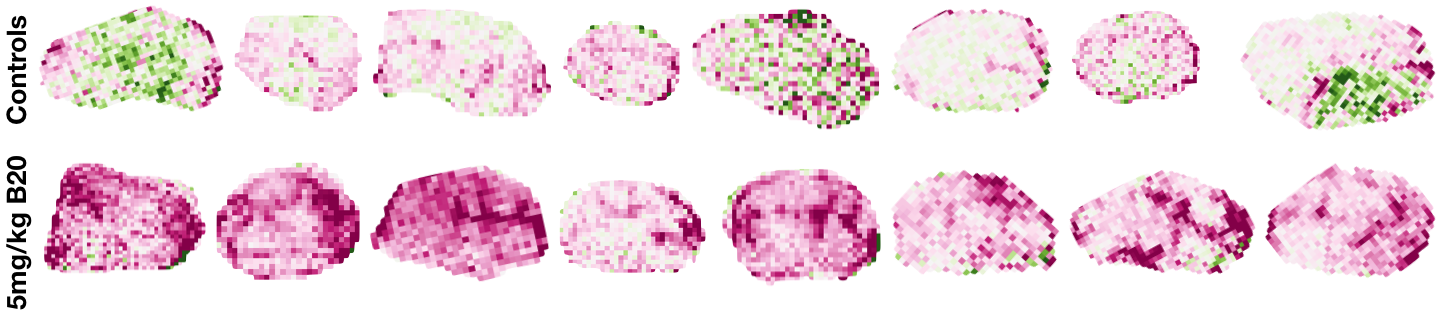
\includegraphics[width=\textwidth]{oemri_thesis3/oemri_thesis3-images/1_aarts3_b20_dOEMRI.pdf} % requires the graphicx package
   \caption{A) \acs{NCWF} maps obtained from \ac{ICA} (\ac{dOE-MRI} maps) are shown for control tumours as well as those treated with 5mg/kg B20 and imaged 48 hours later.
   Of the 10-16 slices for each animal, a representative slice was chosen.
   As indicated by the distribution of purple voxels, control tumours show considerably less response to oxygen than the treated tumours.
   Additionally, regions marked in green are considered to be hypoxic; these regions were not prevalent in the treated tumours.
   B) A representative histology slice from a control and a treated tumour is shown stained with pimonidazole (green) and CD31 (purple).}
   \label{dOEMRImaps}
\end{figure}

\begin{figure}[htbp]
   \centering
   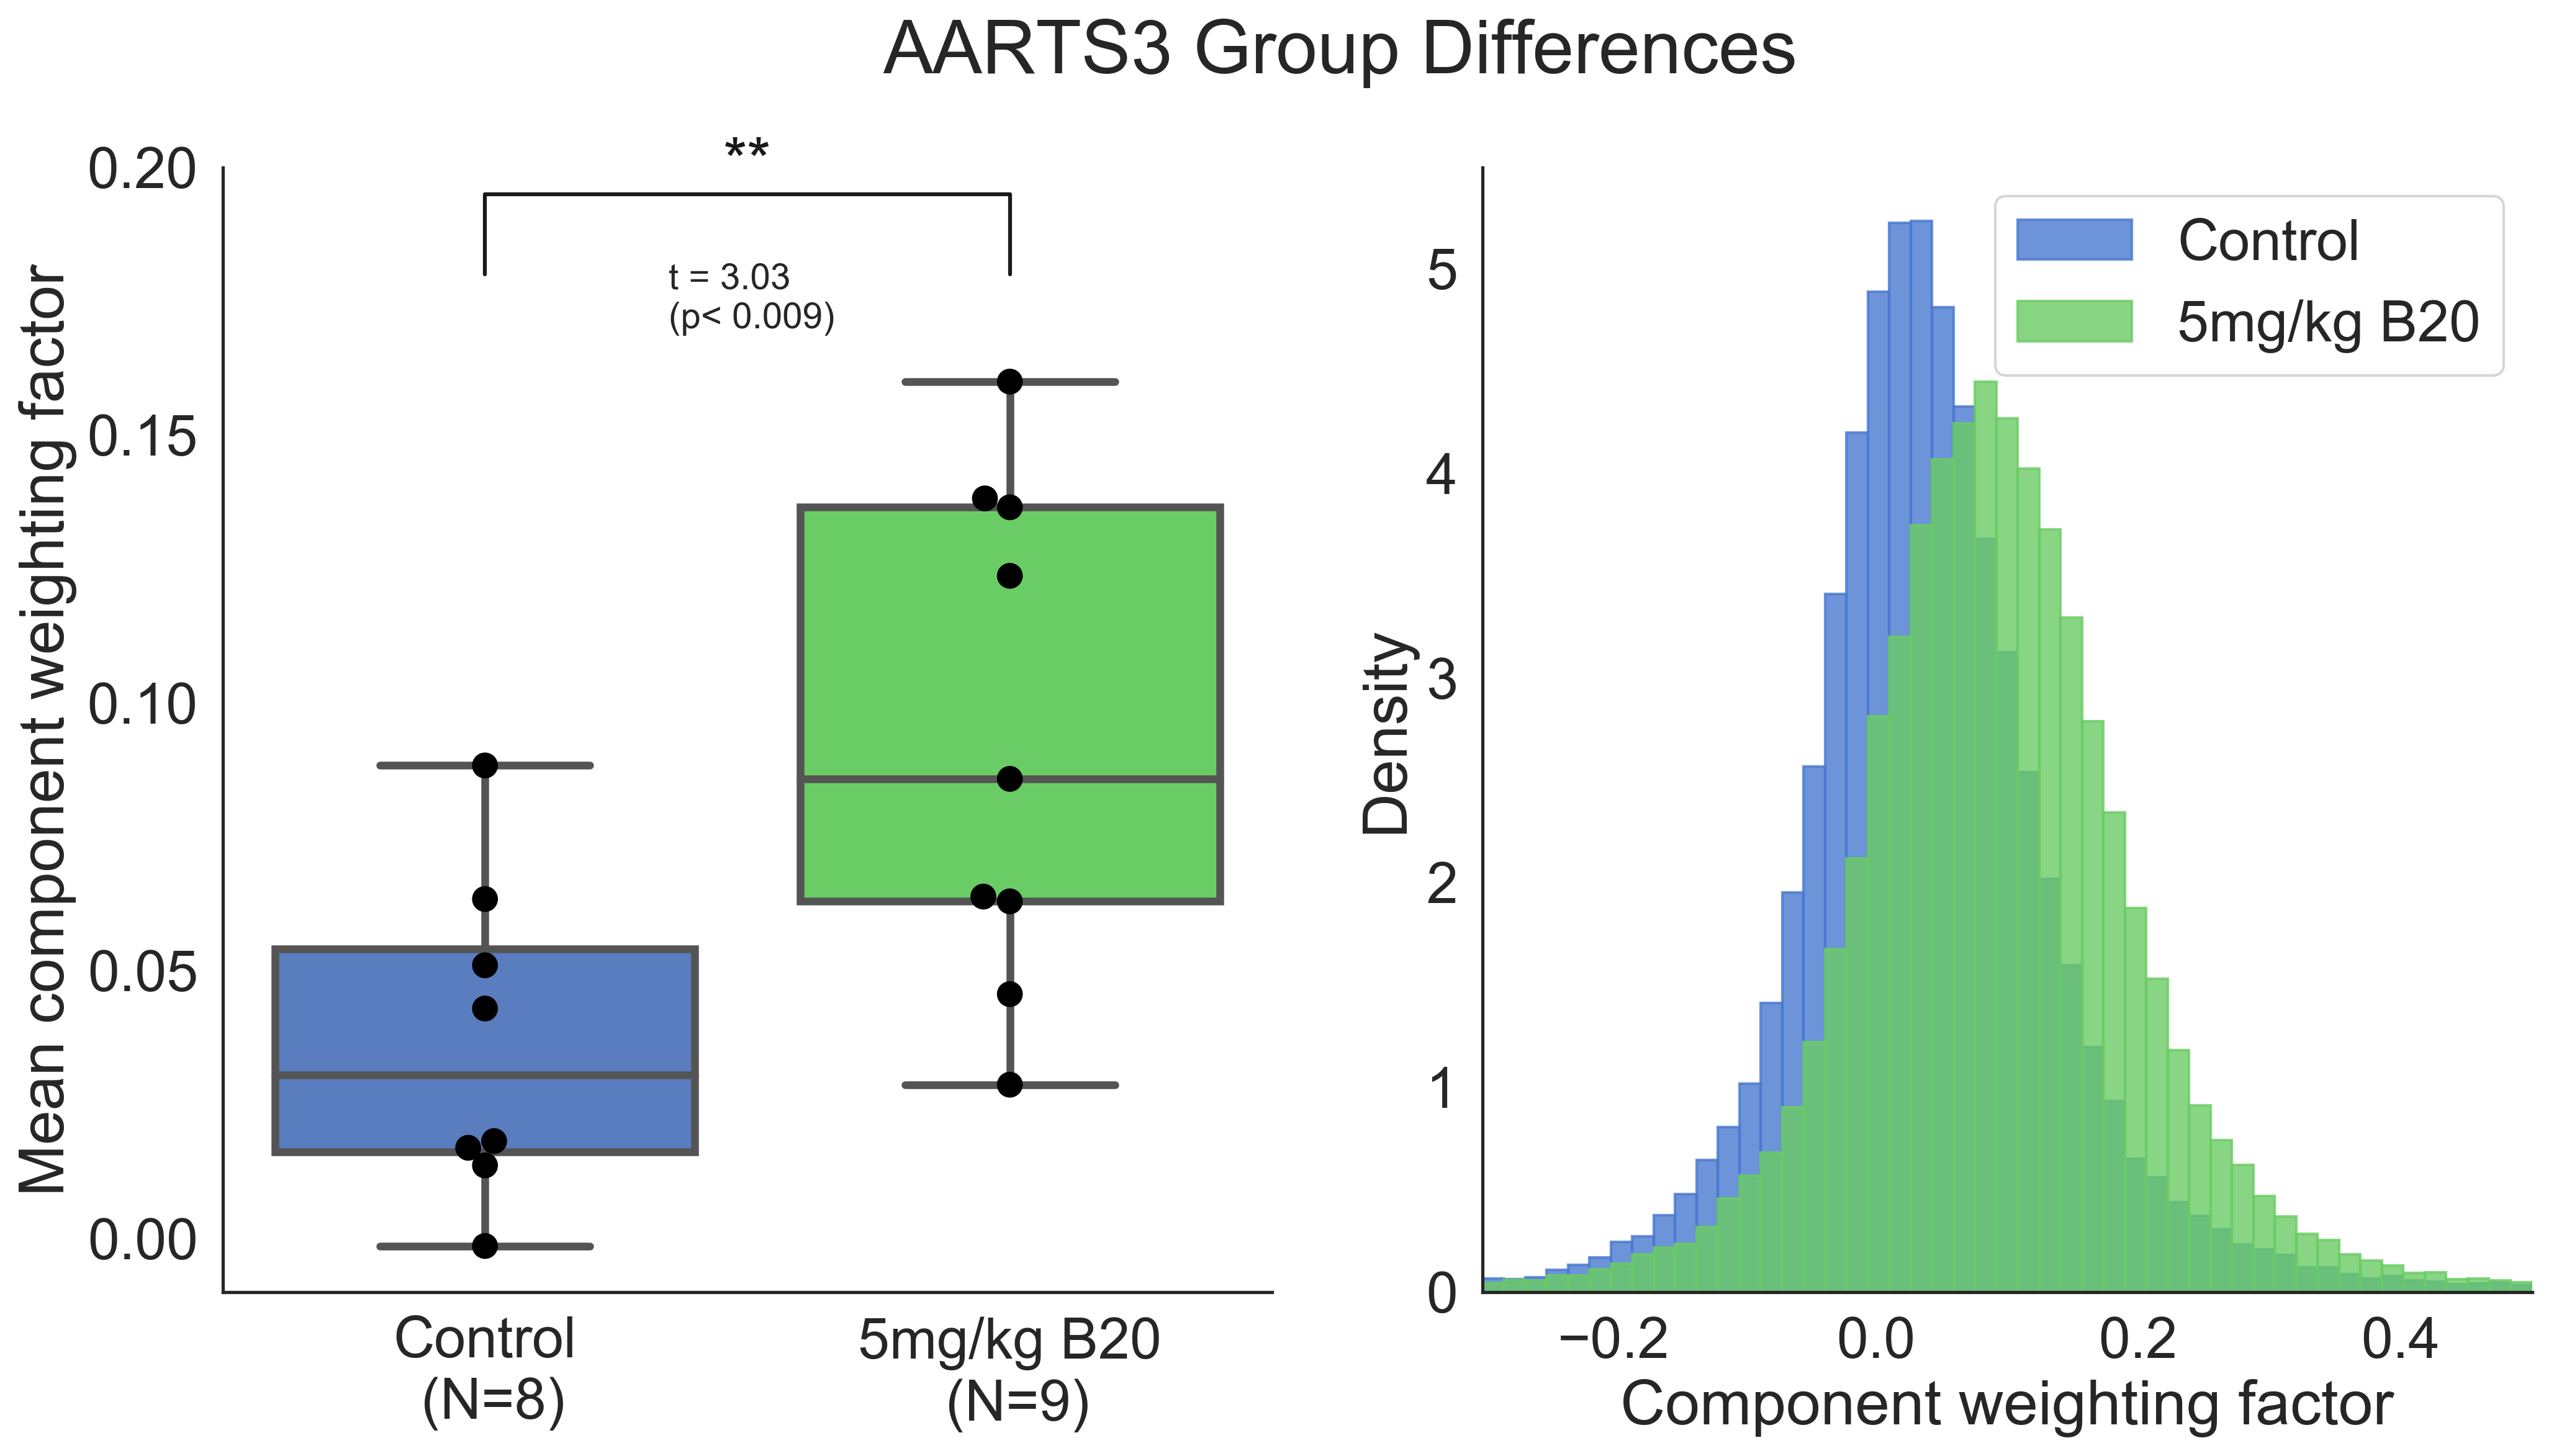
\includegraphics[width=\textwidth]{oemri_thesis3/oemri_thesis3-images/2_aarts3_b20_boxplot_dOEMRI.png} % requires the graphicx package
   \caption{A) Group differences of the normalized mean \acs{NCWF} are shown in a boxplot.
   Each dot represents the mean value of a mouse with the controls in blue and treated in green.
   The differences are statistically significantly different (p=0.0092) with a large effect size (Hedge's g = 1.08).
   B) Density distributions of all voxels shows treated tumours shifting towards increased responsiveness to delivered oxygen (higher \acs{NCWF}).}
   \label{aarts3boxplot}
\end{figure}

\subsection{\acs{IM} tumours have a higher baseline oxygenation level than \acs{SC} tumours from the same cell line}

Tumours implanted at the \acs{IM} site received only 20\% of the cells compared to the subcutaneous tumours to account for faster growth of \acs{IM} tumours.
Figure~\ref{tumourVolumes} shows no statistically significant difference in tumour volumes for any of the groups, control or treated, \acs{IM} or \acs{SC}. 
Across 10 animals and 23 tumours in total, the mean across all groups was $V = 424 \pm 41 mm^3$ (mean $\pm$ sem). 
%Histological sections of the \acs{IM} and \acs{SC} tumours show the microenvironments to be morphologically distinct (figure~\ref{imsc}).\todo[backgroundcolor=red!20!white]{add a couple of sentences about differences in morphology}.
\ac{dOE-MRI} was applied to mice bearing both \acs{SC} and \acs{IM} tumours to evaluate whether tumour implant site affects baseline oxygenation. 
As shown in figure~\ref{OEP8boxplot}, baseline \acs{NCWF} values in \acs{IM} tumours were significantly higher for \acs{IM} tumours compared to \acs{SC} tumours (Mann-Whitney U = 1.0, p = 0.003).
The effect size was large with Hedge's ${g=1.38}$.

\begin{figure}[htbp]
   \centering
   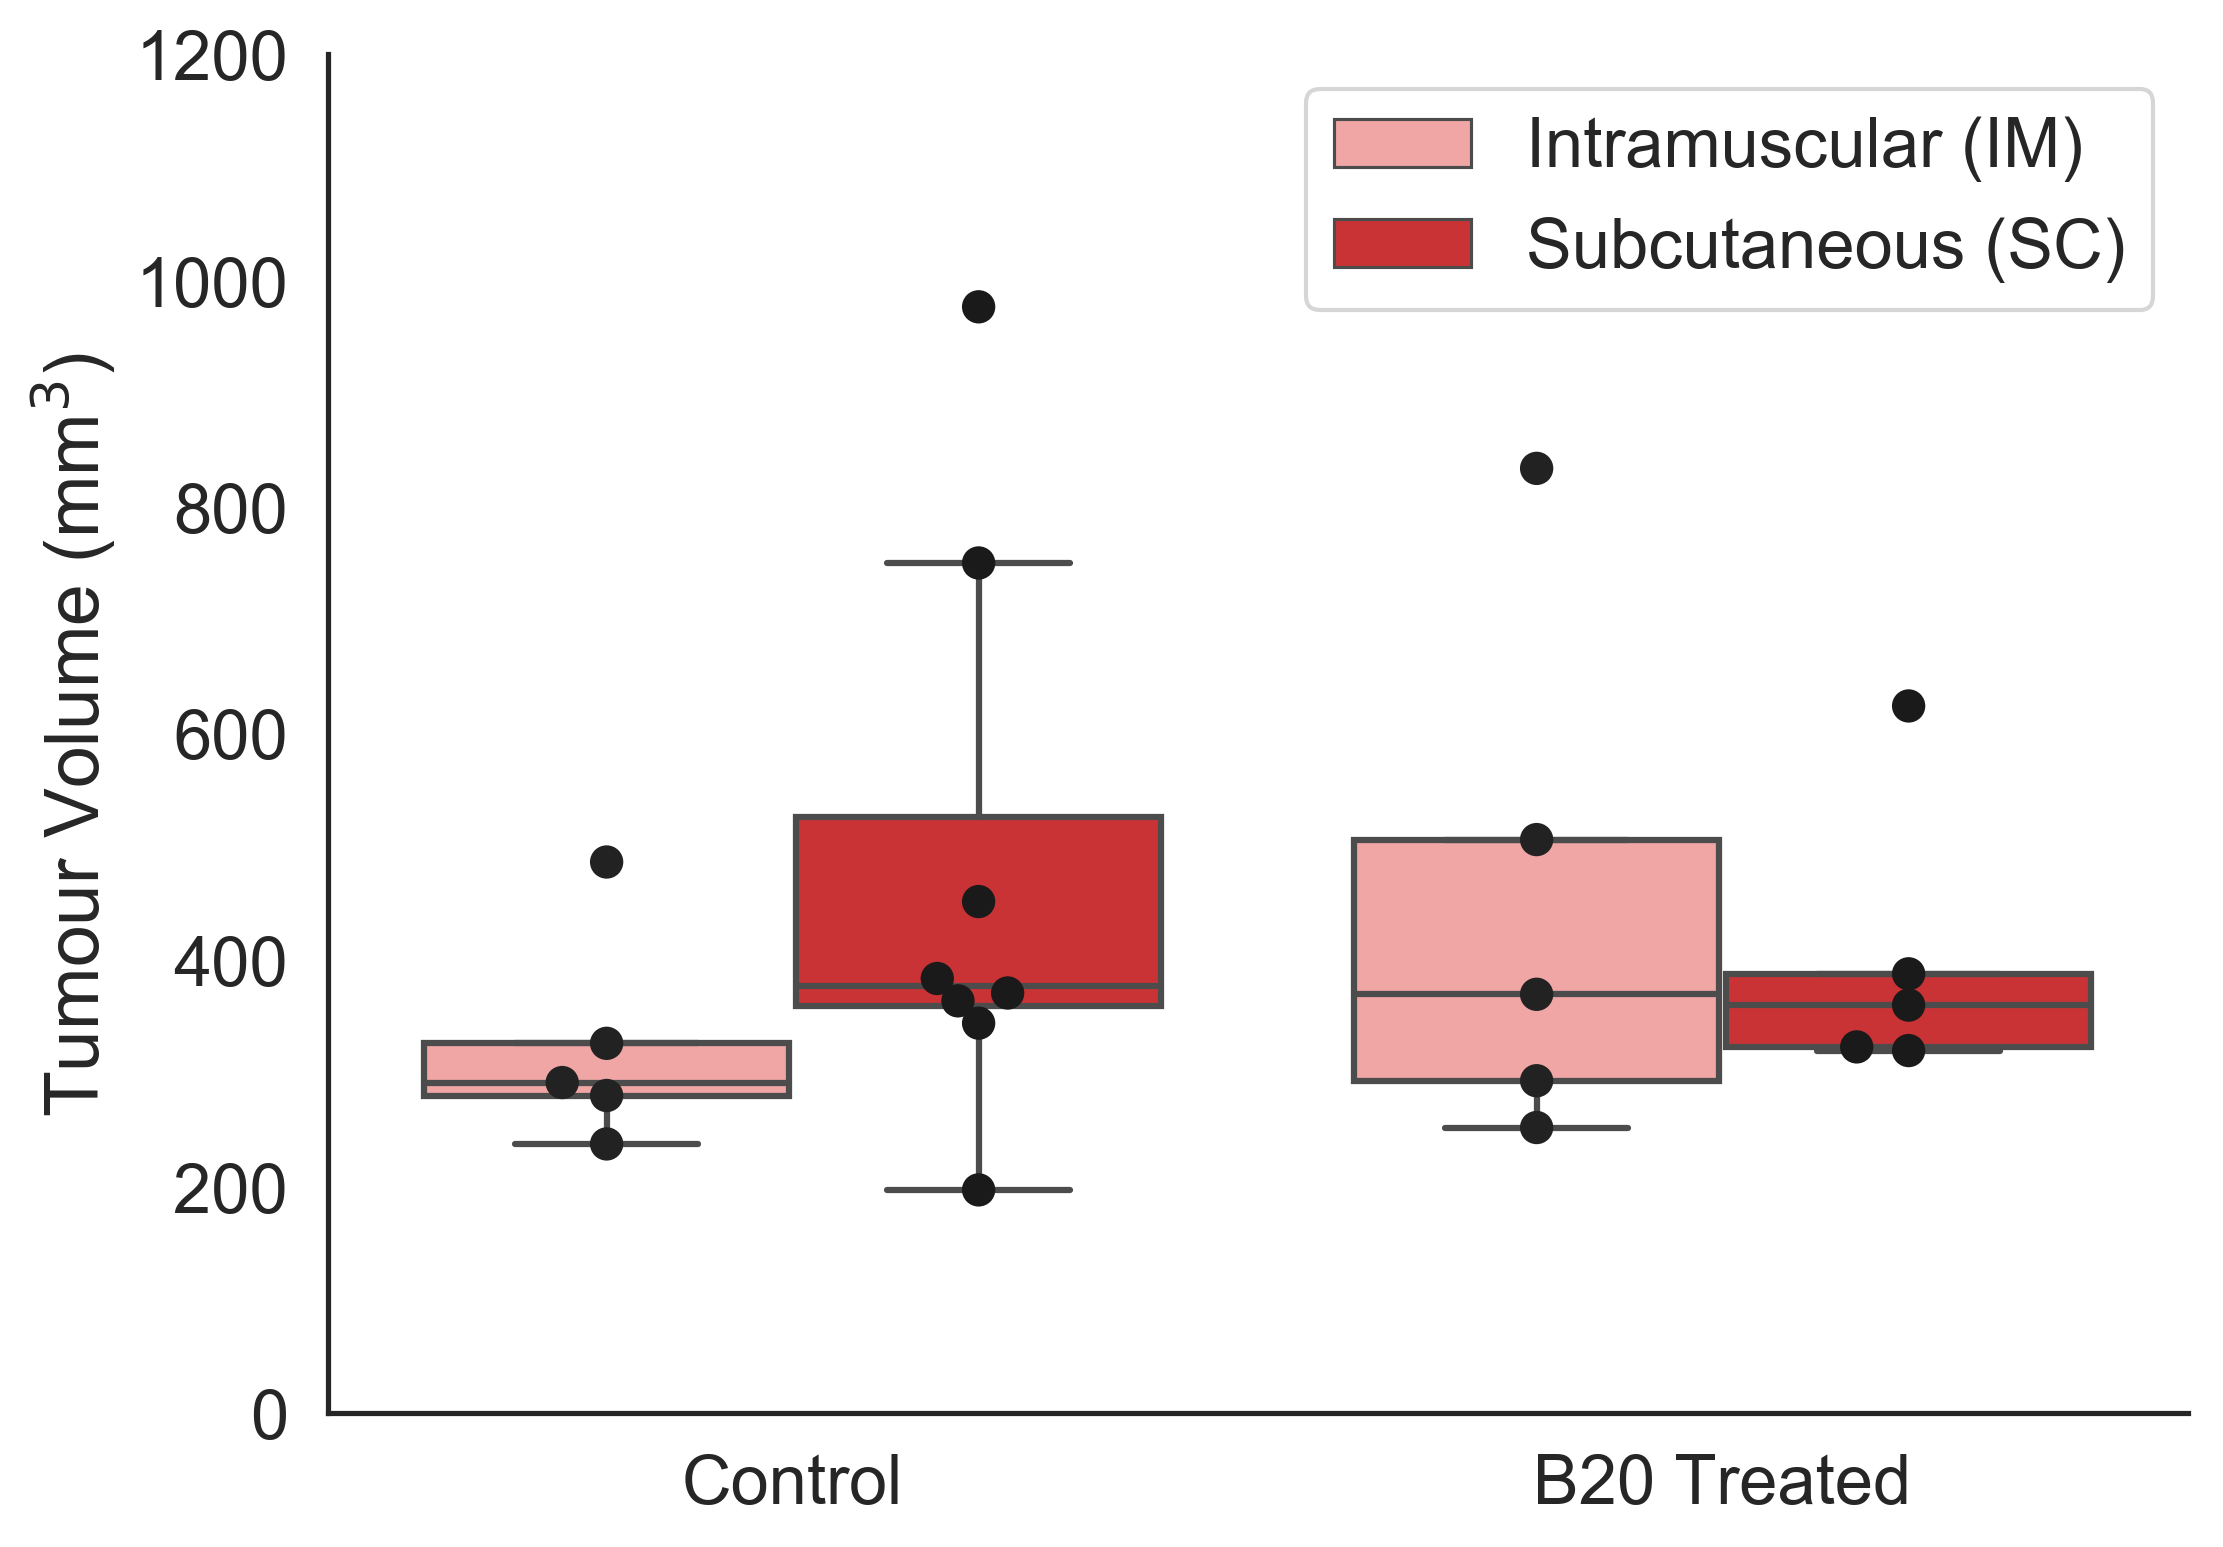
\includegraphics[width=\textwidth]{oemri_thesis3/oemri_thesis3-images/6_oep8_tumourVolumes.png} % requires the graphicx package
   \caption{Calculated tumour volumes from each of the four groups is shown. There were no statistically significant differences in tumour volumes amongst any of the groups.}
   \label{tumourVolumes}
\end{figure}

%\begin{figure}[htbp]
%   \centering
%   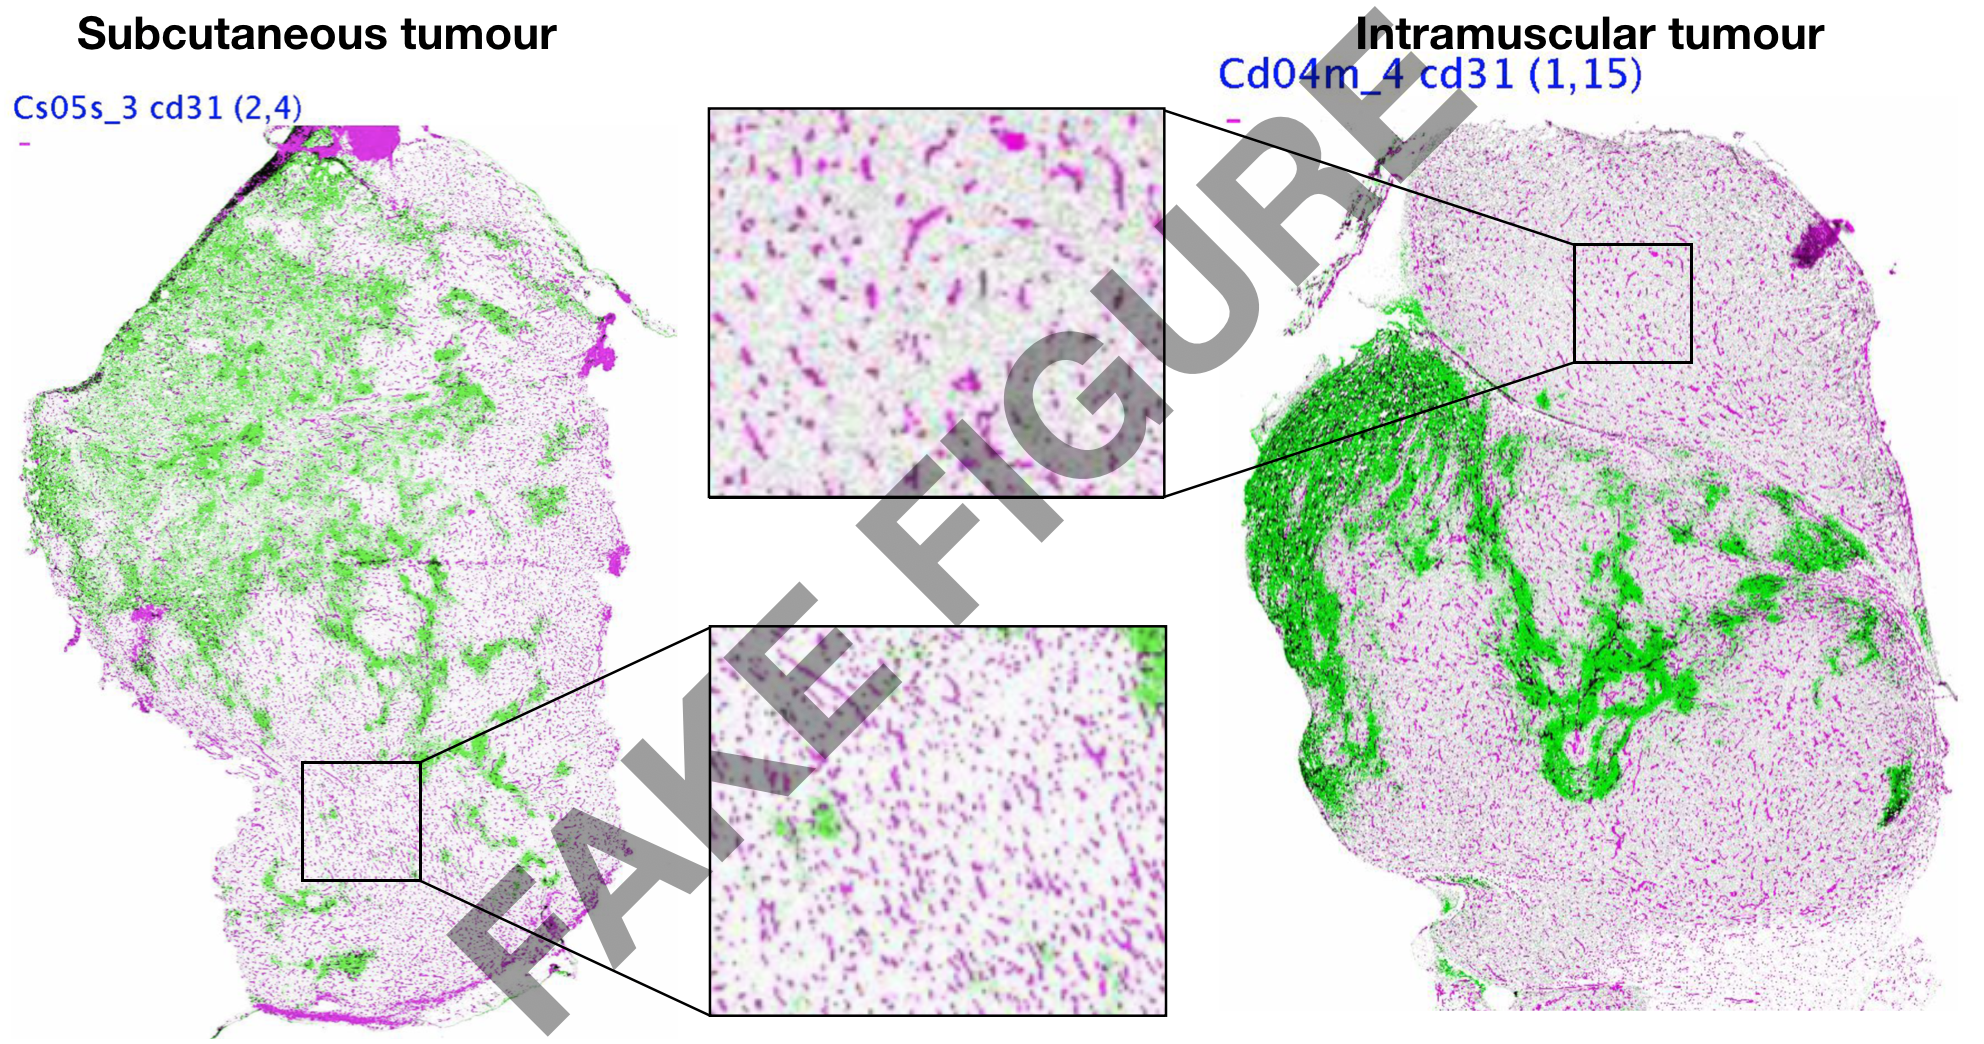
\includegraphics[width=\textwidth]{oemri_thesis3/oemri_thesis3-images/3_imsc_zoomed.png} % requires the graphicx package
%   \caption{example caption}
%   \label{imsc}
%\end{figure}

\subsection{Effects of B20 are dependent on the tumour microenvironment and baseline oxygenation}

To investigate whether the effects of antiangiogenic agents are dependent on different tumour microenvironments, mice were implanted with both \acs{IM} and \acs{SC} tumours. 
Tumours in this experiment were treated 24 hours prior to imaging.
To ensure the \acs{SC} tumours from mice with a double implant were similar to mice with only a single implant, three mice were implanted only with subcutaneous tumours.
No differences were found (data not shown), so the \acs{SC} tumours from this experiment were pooled together.

When comparing between \acs{SC} baseline and treated groups, there was a statistically significant difference (Mann-Whitney $U = 3.0, p = 0.007$) observed in mean \acs{NCWF} values for control (0.073 $\pm$0.009) vs. B20-treated tumours (0.119 $\pm$0.013) with a large effect size: Hedge's ${g=1.77}$ (Fig.~\ref{OEP8boxplot}).
However, no measurable difference in oxygenation was observed for the \acs{IM} tumours after B20 treatment (Mann-Whitney $U = 11.0, p = 0.42$).
Mean \acs{NCWF} from B20-treated \acs{IM} tumours was 0.137$\pm$0.018, and control \acs{IM} tumours was 0.146$\pm$0.017. 
Histological images (Fig.~\ref{allHisto}) also suggests that control \acs{IM} tumours have significantly less pimonidazole staining compared to \acs{SC} controls.
Furthermore, reduction in pimonidazole staining between control and treated \acs{IM} tumours is much lower compared to \acs{SC} tumours.
This provides clear evidence that the effects of B20 are dependent on the tumour microenvironment, and \acs{dOE-MRI} is sensitive to these differences.

\begin{figure}[htbp]
   \centering
   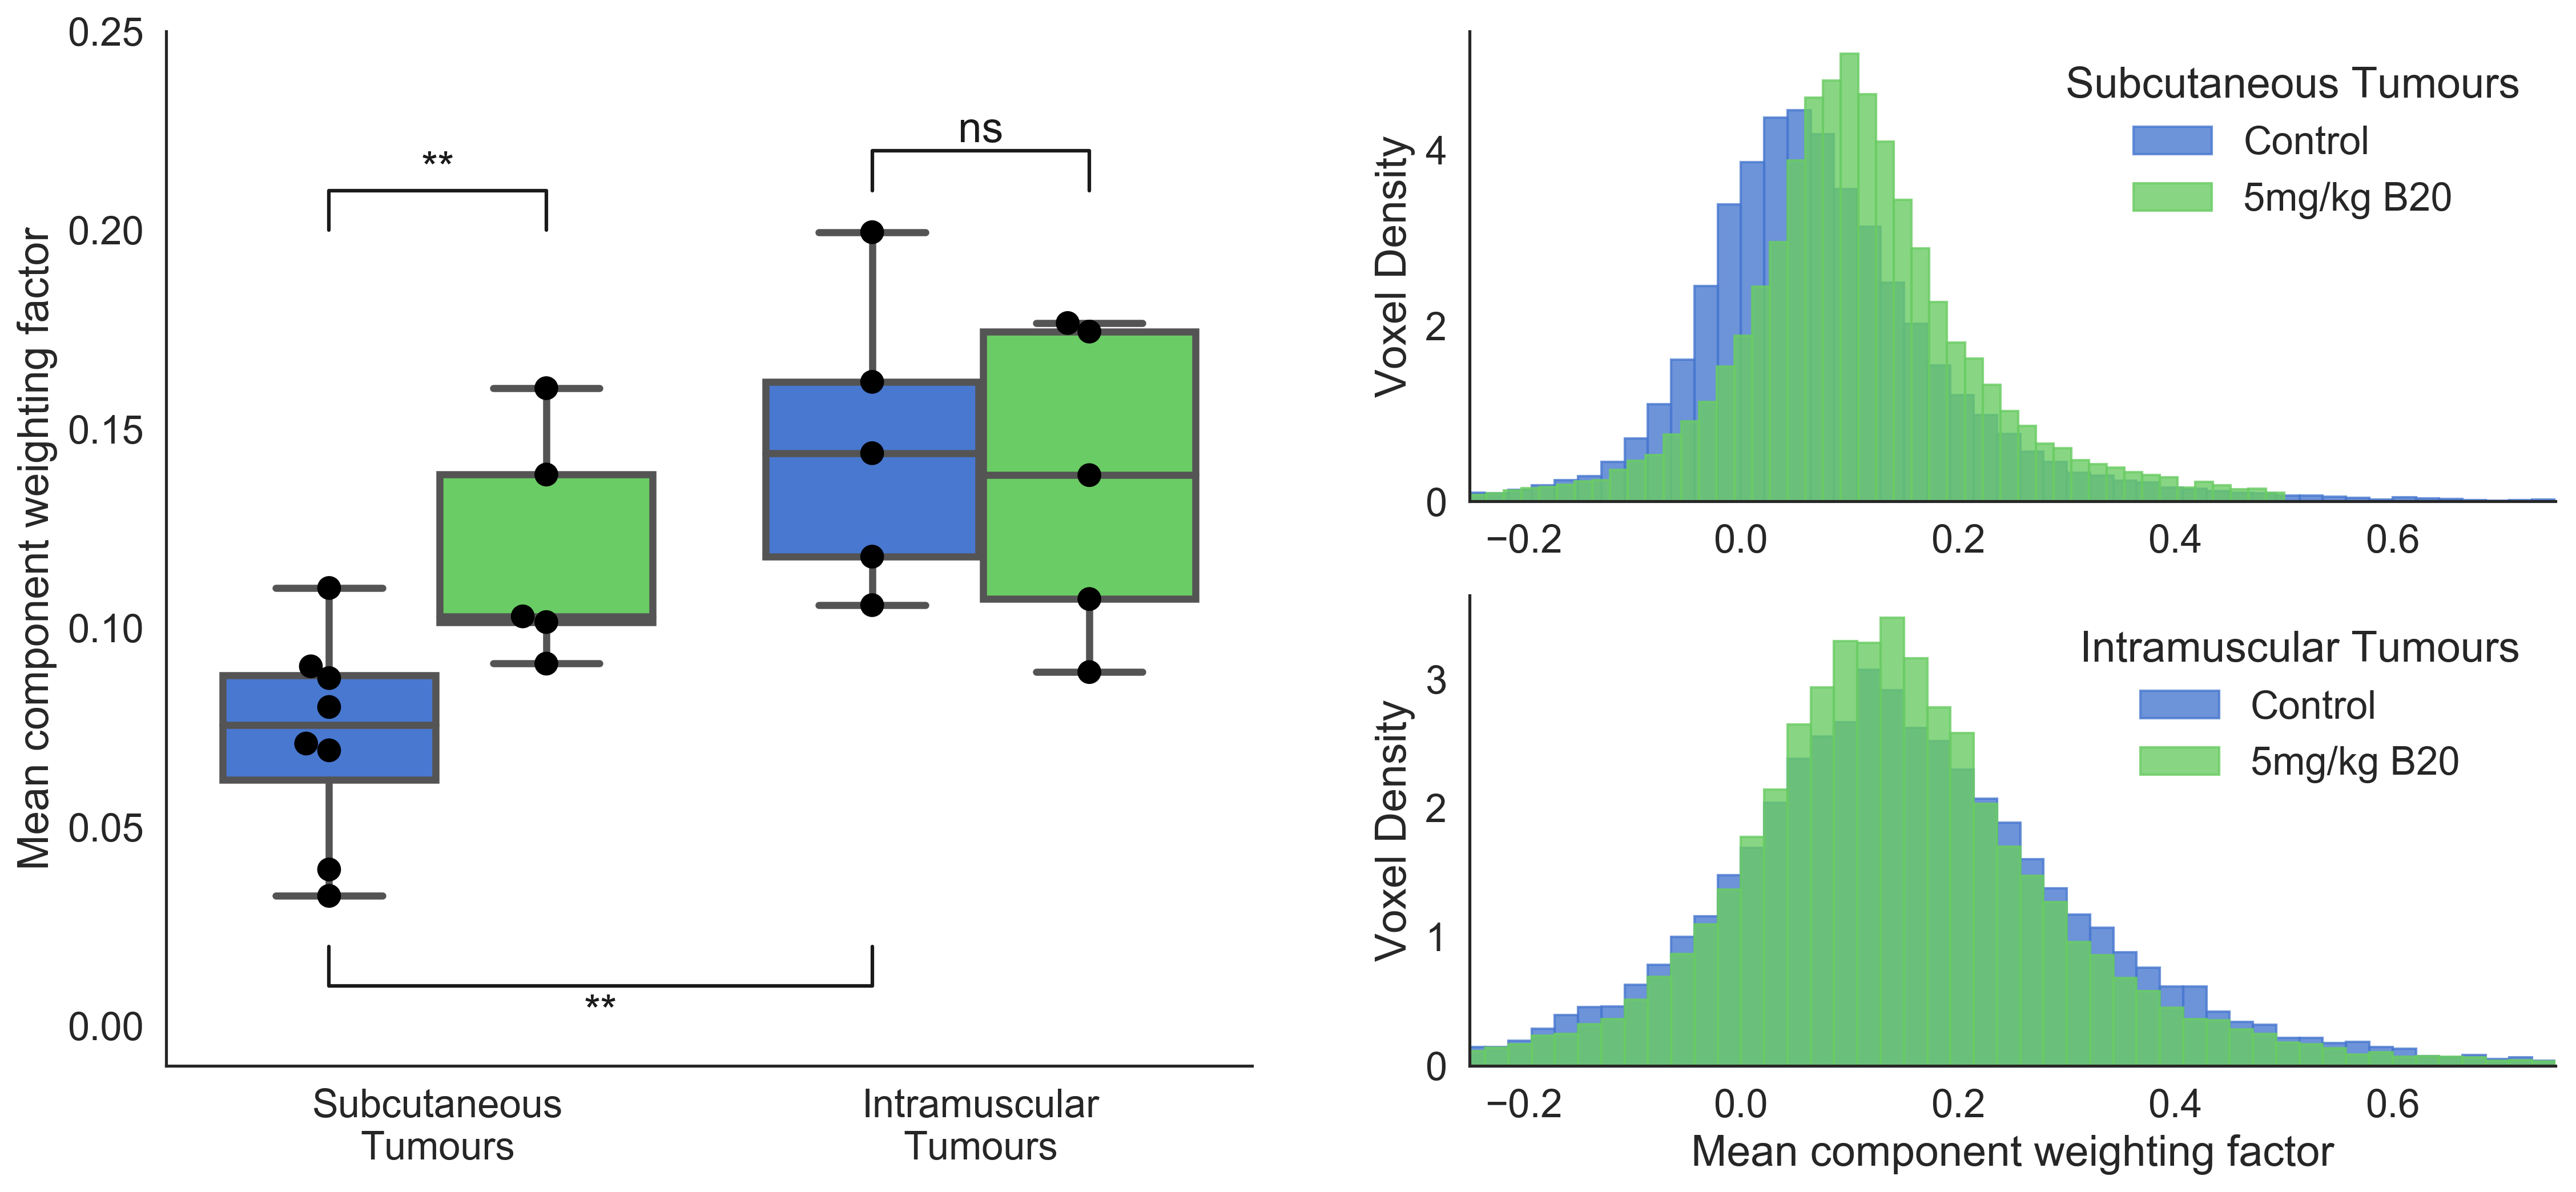
\includegraphics[width=\textwidth]{oemri_thesis3/oemri_thesis3-images/4_oep8_IMSC_b20_sanitized_dOEMRI.png} % requires the graphicx package
   \caption{\textbf{A)} Boxplot with four groups, 5mg/kg B20 treated and control mice with both \acs{SC} and \acs{IM} tumours.
   Differences between control \acs{SC} and \acs{IM} tumours, as well as control \acs{SC} and treated \acs{SC} tumours are statistically significant (Mann-Whitney U test; p $<$0.005, marked as **).
   There was no significantly difference in treated and control \acs{IM} tumours.
   \textbf{B)} Voxel density distributions of \acs{NCWF} for \acs{SC} (top) and \acs{IM} (bottom) treated and control tumours.
   Density distribution (i.e. normalized histograms) are shown rather than voxel counts due to uneven group size. 
   Note the shift of the \acs{IM} control tumours towards a higher \acs{NCWF} value.}
   \label{OEP8boxplot}
\end{figure}

\begin{figure}[htbp]
   \centering
   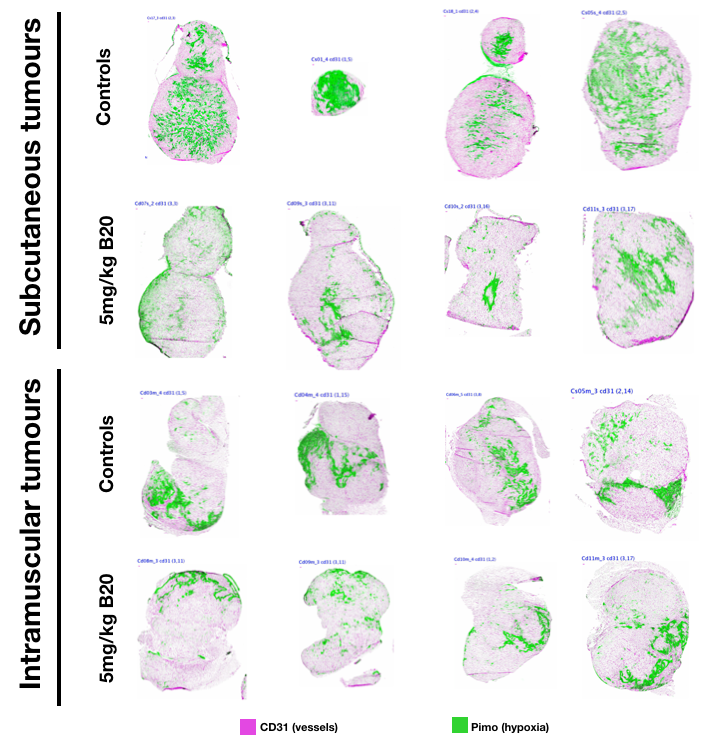
\includegraphics[width=\textwidth]{oemri_thesis3/oemri_thesis3-images/5_oep8_imsc_histo.pdf} % requires the graphicx package
   \caption{Representative histological sections from 16 total tumours of all four groups: 5mg/kg B20 treated and control mice with \acs{SC} and \acs{IM} tumours.
   Hypoxia marker pimonidazole staining is shown in green, and purple indicates the presence of blood vessels stained by CD31.}
   \label{allHisto}
\end{figure}

% ======================================================================
\section{Discussion}
% ======================================================================

% Bits and pieces from the latest grant pulled into this first paragraph
Hypoxic tumour cells may arise due to proliferation of cancer cells outpacing the growth of new vasculature, increasing the separation between blood vessels and forcing cells beyond the diffusion distance of oxygen from the blood supply. 
An alternative route to hypoxia is the consequence of poor flow, which can result in hypoxic tumour tissue due to depleted oxygen supply in the flowing blood or due to intermittent flow of poorly formed vessels. 
Tumour microenvironments are dynamic and highly heterogeneous, with variable vascular function and patterns of hypoxia.
However, the importance of hypoxia in tumours is well validated and undisputed; a meta-analysis of tumours from multiple origins found a consistent relationship between greater hypoxia in tumours and poorer outcomes with radiotherapy~\cite{Horsman:2012kw}.
While many techniques exist for measuring hypoxia in tumours, none have become clinical routine mainly owing to their expense, poor sensitivity and specificity, limited availability or their invasive nature~\cite{Colliez:2017fc,Baumann:2016gr}. 
For example, Eppendorf electrodes are sensitive and specific, and are a gold standard of measuring tissue hypoxia, but they are highly invasive, limited by sampling, and are not widely available. 
The accelerated radiotherapy, carbogen and nicotinamide (ARCON) trial demonstrated benefit in hypoxic tumours assessed retroactively using pimonidazole labeling of biopsy samples~\cite{Kaanders:2002wl}. 
However, immunohistochemical analyses of markers of hypoxia such as pimonidazole are invasive and do not sample the entire tumour.
A more widely applicable hypoxia-measuring tool that overcomes the availability, expense, invasiveness, sensitivity and specificity hurdles would be of high value for stratifying patients in hypoxia-targeted trials, prognostic imaging as well as for monitoring response to treatment. 

In this study we have demonstrated the utility of \acs{dOE-MRI} to assess tumour oxygenation changes after administration of B20.
Though this is not the first report of tumour oxygenation improvements after antiangiogenic drug treatment using MRI methods, we provide clear evidence this change is measurable using only the switching of inhaled gas and no injectable contrast agents.
Using electron paramagnetic resonance and an injectable paramagnetic tracer (triarylmethyl radical derivatives), Matsumoto et al.\ mapped increases in the partial pressure of oxygen in tumours after administration of the VEGF inhibiting antiangiogenic agent called sunitinib.
Two to four days following antiangiogenic treatment with sunitinib, they reported a transient improvement in oxygenation~\cite{Matsumoto:2011iv}.
Lemasson et al.\ obtained estimates of blood oxygen saturation using an ultrasmall super-paramagnetic iron oxide (\acs{USPIO}) contrast agent in a rat gliosarcoma model.
They reported that after sustained administration ($>$9 consecutive days) of the maximum dose of sorafenib, oxygen saturation in treated tumours reduced compared to untreated control tumours~\cite{Lemasson:2012dl}.
In this case, the dose and treatment schedule resulted in excessive pruning of the tumour vasculature to the point where drug and nutrient delivery became limited and tumour oxygenation actually reduced~\cite{Jain:2013jc}.
In our experiments, with the dose (5~mg/kg) and treatment schedule (single administration 24 or 48~h prior to imaging), we expected a vascular normalization effect corresponding to an increase in oxygenation~\cite{Chauhan:2012bm,Jain:2013jc,Huang:2012kn}.
Despite heterogeneity in amount and levels of oxygen response in the \acs{SC} tumours, we observed an overall increase in oxygenation after administering B20 (figures~\ref{dOEMRImaps},~\ref{aarts3boxplot}, and~\ref{OEP8boxplot}).

In this study we provided evidence that the location of tumour cell implants has a large impact on the microenvironment of the resulting solid tumour.
Tumour kinetics and responses to chemotherapies differ depending on the implant site and the effect of tumour implantation site is often not considered when assessing drug effect using \emph{in vivo} animal studies~\cite{Arjona:2006ch}.
Hubbard et al.\ compared the tumours derived from the VX2 rabbit carcinoma line implanted intramuscularly and intra-abdominally and discovered animals with \acs{IM} tumours had significantly higher levels of calcium compared to animals with intra-abdominal tumours~\cite{Hubbard:1980vf}.
This result was attributed to the differences in venous drainage of the two sites.
In another example, Malave et al.\ studied the Lewis-lung carcinoma model and reported a lower implant success rate for tumours implanted in the flank compared to the foot pad, and a higher rate of metastatic modules for tumours in the flank (indicating a reduced tumour-host immune response)~\cite{Malave:1979ui}.
Tumour implant site also alters growth kinetics and dramatically different tumour doubling times (in days) has been reported for implants in mouse tail (1.7), foot (1.6), chest (1.2), and leg (0.6)~\cite{Hill:1982ci}.
For the same amount of cells implanted, our experience is that \acs{IM} tumours typically grow much faster, have a more stable vascular architecture, less hypoxia (pimo staining), and increased vessel density (CD31 \%).
We attempted to control for this growth rate by injecting fewer cells for the \acs{IM} tumours. 
Our tumour volume measurements indicate there was no significant difference between the control \acs{IM} and \acs{SC} tumours despite the \acs{SC} tumours implanted with 5 times the amount of cells implanted.
We also showed that \acs{dOE-MRI} can assess increased baseline oxygenation in control tumours when the tumour site is changed from the dorsal subcutaneous region to the hind limb: \acs{IM} tumours have less pimonidazole staining compared to \acs{SC} tumours (figure~\ref{allHisto}).
%Figure~\ref{imsc} highlights some of these differences in representative SCCVII  tumours implanted \acs{SC} and \acs{IM}~\todo[backgroundcolor=red!20!white]{add some differences about tumours}.
Ultimately we showed that following treatment of \acs{IM} tumours with B20, no change in oxygenation was observed, likely because \acs{IM} tumours were already well-oxygenated.

To fully establish the utility of \acs{dOE-MRI} to assess tumour oxygenation non-invasively using inhaled oxygen or air, several subsequent experiments should be conducted.
Some ambiguities remain with a T$_1$-based \acs{dOE-MRI} method as its reflection of dissolved O$_2$ concentrations is complicated by complex, non-linear relationships with hemoglobin saturation and its effects on T$_2^*$, and with vascular perfusion and blood flow that may confound interpretation of existing \acs{dOE-MRI} signal.
These are further complicated by the array of physiological possibilities that may be visualized by a change in T$_1$. 
In future development of this method, the impact of T$_1$-weighting should be explored to ensure effects of interventions are not manifesting due to changes in tumour microenvironment that alter T$_1$.
An increase in T$_1$ suggests an oxygen-responsive area, while non-responding and negative-responding regions may represent a variety of physiologies. 
These areas may be completely unperfused and even necrotic, or they may be poorly perfused but viable, hypoxic tissues.
Further exploration of intermediate regions (i.e. not hypoxic or well-oxygenated) using \acs{dOE-MRI} and coupling it with \acs{BOLD}-MRI is warranted to fully classify all areas of the tumour. 
An unexplored application of \acs{dOE-MRI} is its potential to monitor treatment efficacy longitudinally as the contrast mechanism used is completely reversible. 
This opens up the possibility to do treatment interventions within a single imaging session with perfectly co-registered tumour volumes to allow for assessing oxygenation changes at the level of a single voxel.
Nevertheless, \acs{dOE-MRI} has tremendous potential for assessing tumour oxygenation as a non-invasive imaging method that is urgently needed in the clinic. 

% ======================================================================
\section{Conclusions}
% ======================================================================

Through this work we have shown that subcutaneously implanted SCCVII tumours treated with B20 and imaged 48h later are more oxygenated than control tumours. 
Additionally, we have established \acs{dOE-MRI} as a tool to assess baseline oxygenation level and demonstrated that \acs{IM} tumours are significantly more oxygenated than \acs{SC} tumours implanted in the same mice.
Finally we provided evidence that location of the tumour implant site has a large effect on therapy outcome as the more oxygenated \acs{IM} tumours did not respond to treatment with B20.
It is our expectation that after further refinement and expansion, this technique will become accessible and available in the clinic to screen cancer patients prior to chemo- or radiotherapy prescription, and be useful for developing new hypoxia-targeting drugs.





%% The following is a directive for TeXShop to indicate the main file
%%!TEX root =../diss.tex

\chapter{Future Work}
\label{ch:futurework}

\section{Exploring the link between perfusion and oxygenation}

\subsection{Comparing DCE-MRI perfusion patterns with \ac{dOE-MRI} oxygenation patterns}

One SCCVII and one HCT-116 tumour-bearing mouse were catheterized and injected with 30mM solution of Gd-DTPA for DCE-MRI at a rate of 1mL/min using a power injector at a dose of 5$\mu$L/g.

\noindent\textbf{Perfusion maps:} Signal intensity timecourse from the DCE-MRI map was first normalized to the mean signal intensity pre-injection.
Area under the first 60 seconds of the normalized signal intensity enhancement curve after the injection was calculated (\acs{AUC}$_{60}$) using the composite Simpson's Rule (\texttt{scipy.integrate.simps}).
A binary ground-truth perfusion map was constructed by classifying all voxels with IAUC$_{60} > 0$ as perfused and everything else as unperfused.

Where \ac{dOE-MRI} and DCE-MRI scans were acquired in the same SCCVII and HCT-116 tumour-bearing mice,  maps of oxygenation status were compared to IAUC$_{60}$ perfusion maps, as shown in Figure~\ref{fig_perfusion}.
Mean IAUC$_{60}$ for the well-perfused SCCVII tumour was 22 $\pm$ 16 \%$\cdot$s and for the comparatively poorly perfused HCT-116 tumour was 7$\pm$ 7 \%$\cdot$s.
Well-oxygenated O$_2$-positive regions generally correspond to perfused, high IAUC$_{60}$ areas in both SCCVII and HCT-116 tumours.
A large patch of necrosis, as identified in histological section, in the HCT-116 tumour was also extremely poorly perfused; such large patches of necrosis were not present in the SCCVII tumour.

\begin{figure}[htbp]
   \centering
   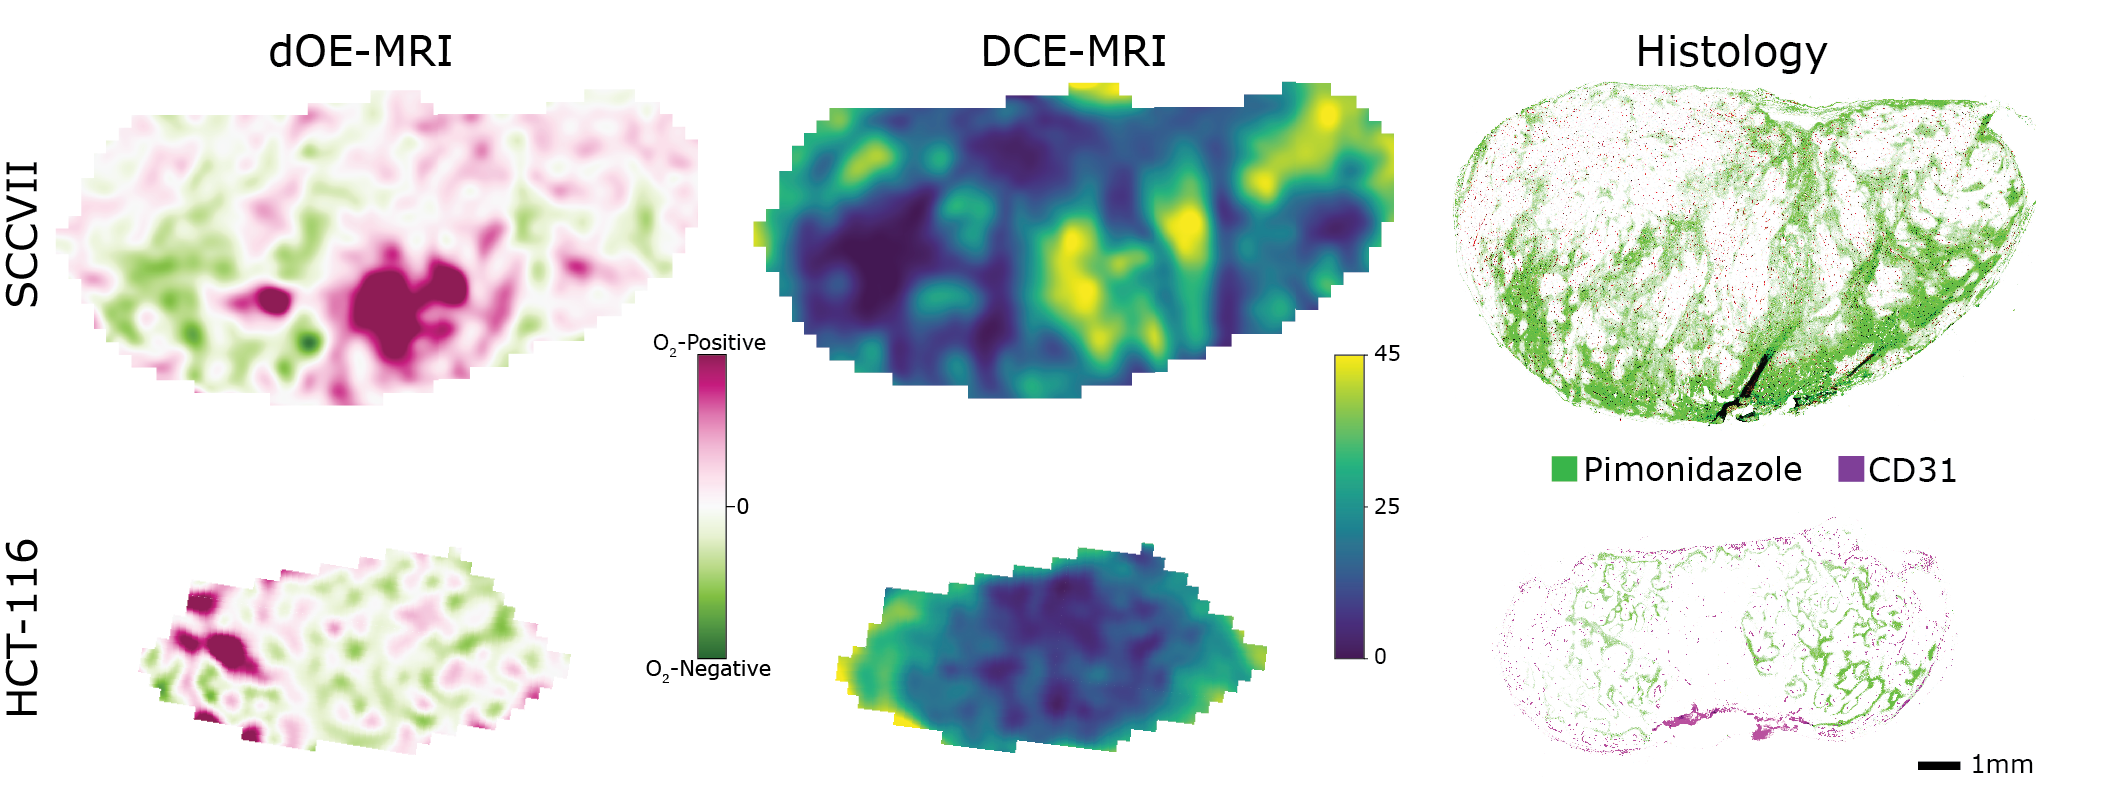
\includegraphics[width=\textwidth]{futurework/futurework-images/fig_perfusion.png} % requires the graphicx package
   \caption{\ac{dOE-MRI} maps and DCE-MRI IAUC$_{60}$maps and slice-matched histology sections of SCCVII and HCT-116 tumours. Large regions marked as purple in the \ac{dOE-MRI} maps are O$_2$-positive and also correspond to regions that have high IAUC$_{60}$ values (yellow). Green or O$_2$-negative regions from the \ac{dOE-MRI} map are often consistent with unperfused regions in the IAUC$_{60}$ (black), but there are regions of mismatch. Histology images stained with pimonidazole (green) and CD31 (purple) are shown for corresponding sections.
   \label{fig_perfusion}}
\end{figure}

\section{Adding T2* to the mix}

%%% from the grant
\todo{this is currently cribbed from the grant, it needs to be DRASTICALLY shortened, and edited for appropriateness, receptiveness, and overall style}
An alternate approach is to simultaneously acquire R1-weighted and R2*-weighted data to improve specificity of the technique[21]. R2* imaging would utilize the Blood Oxygen Level Dependent (BOLD) effect, which can measure shifts in hemoglobin saturation through changes in R2* and therefore assess tumour perfusion without the need for injectable contrast agents. Applying an oxygen challenge also shifts the haemoglobin saturation and, thus, the R2* signal. A postulated biophysical mechanisms is shown in Appendix Fig A2. The expected behaviour of a joint change in R1 and R2* in response to a gas challenge, and how this can be interpreted to reflect tumour oxygenation is based on data from last year?s work by Little et al.[21] and Waterton et al.[23]. The altered R2* provides a robust measure of areas with functioning vasculature. Subsequently, dOE-MRI maps can be masked using the ?R2* maps to exclude unperfused regions and enable improved SNR for R1-weighted signals, resulting in a completely endogenous technique to assess tumour oxygenation. OE-MRI T1-weighted signal more directly reflects oxygen amounts in plasma and tissues and is more applicable for measuring tumour oxygenation as it relates to radiotherapy.
Without sacrificing the information obtained from R1-weighted signal intensity in our current work, it is possible to extract both R1-weighted signal intensity and R2* simultaneously using a dynamic, multi-gradient echo in place of a dynamic FLASH sequence. We propose that our cycling gas challenge in combination with ICA improvement to R1-weighted OE-MR imaging may also be applicable to R2*, and we will test them in combination as an approach to improve the specificity of OE-MRI and therefore increase its capacity for clinical application. 
We propose to further develop dOE-MRI as a biomarker of the tumour microenvironment using simultaneous R1 and R2* imaging: vector-dOE-MRI. This proposal is a logical continuation of the OE-MRI efforts in the Reinsberg and Minchinton labs. The expected outcomes are an important part of a wider hypoxia-targeting effort. A previous grant application with Minchinton as nominated PI has been significantly simplified and re-focussed on the method-development aspect.

%% from approaches & methods

In achieving Objective 1 we will prove that (hypothesis 1) 	our current ICA approach to extract R1-dOE-MRI can be applied to oxygenation-induced changes to R2* from the multi-gradient echo.

In preliminary work we have established that a multi-gradient echo (MGE) sequence is ideal to extend our current R1w dOE-MRI technique [3] to also acquire dynamic R2* data: Initial echoes from an MGE sequence are  R1w and as the echo time increases, the images become more R2*W. The R1w-dOE-MRI map will be calculated from the signal
intensity of the first gradient echo image (minimal echo time TE=2.25 ms). The R2*- dOE-MRI map will be created by applying ICA to the mono-exponentially fitted multi-gradient echo data at each repetition. Fig 4 outlines our approach to obtain R1- and R2*-based dOE-MRI maps from a single multi-gradient echo sequence. Our current experience shows that while the temporal resolution of the multi-gradient echo technique is lower, the data quality of the R1w-dOE-MRI map is not compromised until subsampling exceeds six times the original temporal resolution when compared to that obtained with a FLASH sequence. Details on the impact of lower time resolution are in Appendix Fig A3.
To test our hypothesis we will conduct an imaging study that pits our established FLASH acquisition and ICA technique against the new approach of multi-gradient echoes in a panel of tumour xenograft models exhibiting varying patterns of hypoxia and perfusion. Initially, a Look-Locker sequence to measure a baseline R1 map will be acquired (TE/TR=3.0ms/10000ms, individual inversion time=157ms repeated in 25 frames, geometry matched to subsequent image sequences: matrix=128x80, FoV 3.84cmx2.40cm). Each scan will be for a 30 min O2 challenge. For the first 15 minutes, data will be acquired using the standard R1w-dOE-MRI sequence (TE/TR = 2.67 ms/66.7 ms, ?=40�, temporal resolution of 4.3 s with 210 repetitions for a total scan time of about 15 minutes). Then we will acquire images using the multi-gradient echo sequence (first TE=2.25ms with eleven additional echoes every 2.5ms, TR=35ms, ?=15�, 8 slices, matrix 28x64, temporal resolution=18s, 50 repetitions for total scan time of 15min). We expect no difference between the independently acquired R1-dOE-MRI maps (FLASH vs. MGE) beyond the variability that can be observed in the temporal fluctuation during the 15 minutes experiment. For this comparison of FLASH- and MGE-derived R1-dOE-MRI map, we will follow our stability studies that were part of our initial development of the FLASH-based OE-MRI[3].
The numerical data processing required for ICA will be carried out using a suite of in?house software we developed using the python machine learning library scikit?learn[24], specifically sklearn.decomposition.FastICA. Since ICA is a blind-source estimation and no input of an expected response functions is needed, one can take the successful extraction of a component that is temporally synchronized with the oxygen challenge as proof that tissue R2* is responding to the systemic administration of oxygen. While this provides a test for the hypothesis under Objective 1, physiological relevance will be addressed under Objective 3 using comparison with perfusion assessment and histological information.

\begin{figure}[htbp]
   \centering
   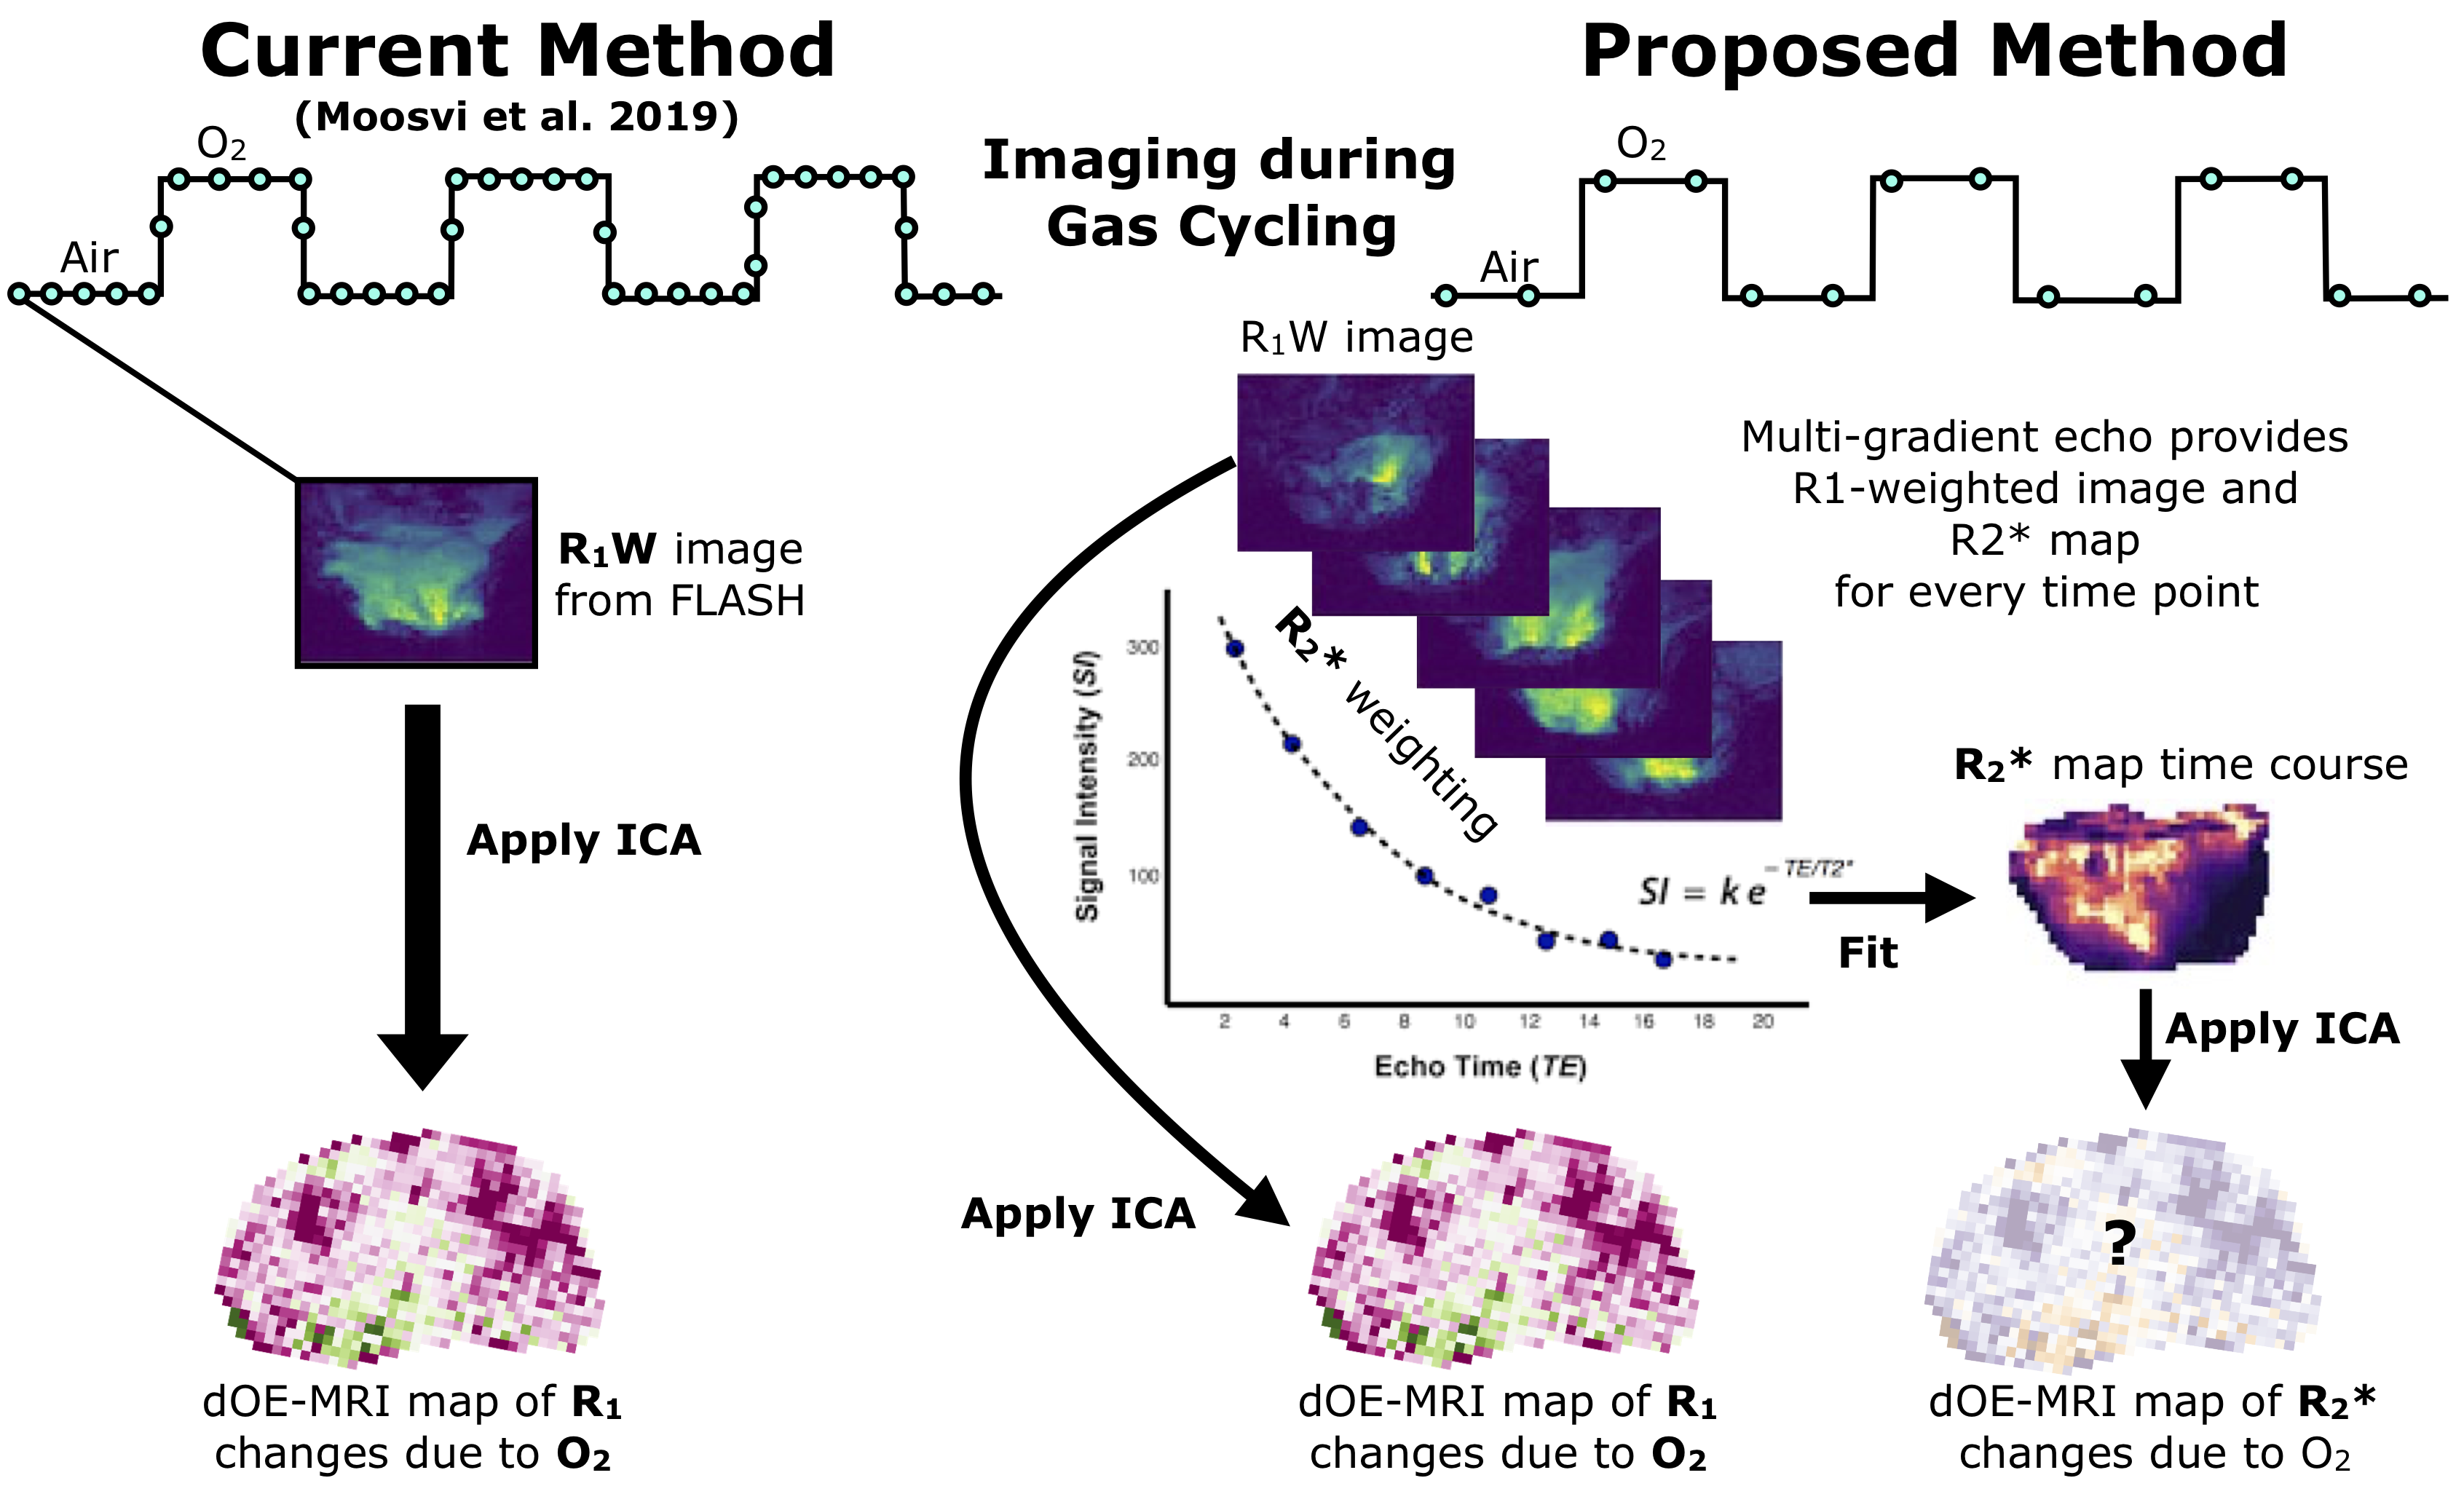
\includegraphics[width=\textwidth]{futurework/futurework-images/grantfig4_MGE_schematic.png} % requires the graphicx package
   \caption{Schematic of the current and proposed acquisition and analysis for \acs{dOE-MRI} with combined R$_1$ and R$_2$ imaging.
   \label{MGE_schematic}}
\end{figure}

\subsection{Independent Vector Analysis}

Our application of ICA to oxygen imaging increased the sensitivity of traditional oxygen-enhanced MRI such that one can investigate oxygen response on a pixel-wise basis rather than having to average R1w signal intensity or T1 changes over regions that are defined by perfusion selection[14,25]. We are planning to investigate whether this enormous gain in statistical power can be replicated by including a further MR parameter (R2*) in a vector-based blind-source estimation adapted from an analysis technique pioneered in fMRI. The problem solved by independent vector analysis (IVA) is that observations that are vector quantities (i.e. tuples consisting of one R1-weighted signal and one R2* from the exponential fit)  are explained by a mixture  of source vectors  [26?28]:

\begin{equation}
x_i = \sum_{j}^{L} a_{ij} \circ s_j
\end{equation}

where $\circ$ indicates an element-wise product. An algorithm suggested by Rafique et al. in 2016 solves the implementation problem and makes it available as FastIVA [29]. This algorithm can be readily implemented in our current analysis framework that makes use of sklearn?s FastICA. We will use FastIVA and analyse the multi-gradient echo data acquired under Objective 1. The independent components synchronized with the oxygen-challenge paradigm will be selected for the extraction of an oxygen-challenge related component map (recall that since this is a blind-source estimation we are not providing an expected response as prior to the analysis). This map will be tested for correlation with aligned tumour sections histologically analyzed for pimonidazole.

A current approach in the use of R1-based oxygen-enhanced MRI is to use a perfusion mask from a contrast-agent injection to exclude unperfused areas. The remaining perfused regions can then be classified into oxygen-refractory and oxygen-enhancing regions[14]. The use of a contrast agent injection complicates the imaging protocol and is being resisted by clinicians[17].
We will acquire MGE data using the sequence developed under Objective 1 and create masks from baseline R2* maps as well as R2*-dOE-MRI maps. Both masks will be applied to R1-dOE-MRI maps obtained through ICA of the first-echo time course from the same MGE data. To validate this technique, we will use the injectable macromolecular contrast agent \acs{HPG-GdF} for a dynamic-contrast enhanced scan. In our previously published methodology we calculated bolus arrival time (BAT), apparent permeability?surface area product (aPS), and fractional plasma volume (fPV) [30]. BAT is a robust marker of tumour vasculature in the use of HPG-GdF. This ?perfusion? parameter map will also be used to mask areas of perfusion within which to evaluate the R1-dOE-MRI map against the histologically evaluated hypoxia marker pimonidazole. When O?Connor et al. validated the R1w-dOE-MRI method, they correlated the oxy-refractory fraction in the perfused areas (regions with positive IAUC60) with pimonidazole staining[14]. We will compare the correlations from perfusion-masked OE-MRI maps (current standard) to the correlations obtained using masking with R2* baseline and R2*-dOE-MRI maps. We will further use the parameter map calculated using IVA (vector-dOE-MRI) as a third contender in the comparison with the current standard.

%%%% End from the grant






%\begin{figure}[htbp]
%   \centering
%   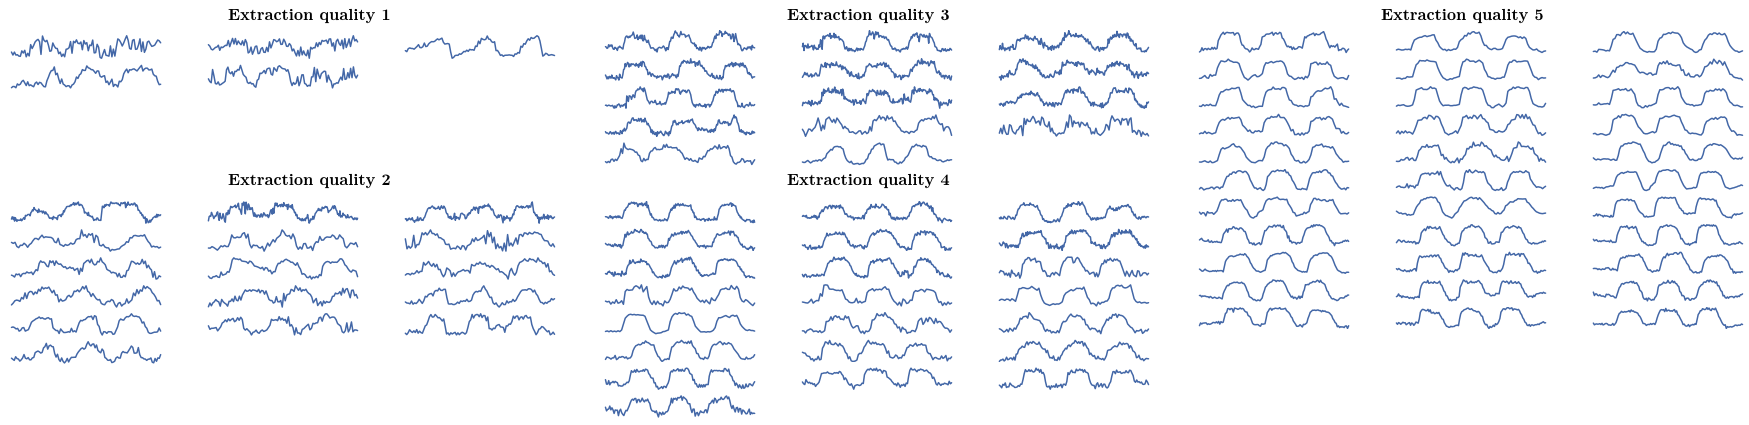
\includegraphics[width=\textwidth]{futurework/futurework-images/technical_ScoredExtractions.png} % requires the graphicx package
%   \caption{Each trace plot is the extracted ICA component corresponding to the oxygen response. The components are scored by the observer from a score of 1 to 5, with 1 barely corresponding to the oxygen challenge with a lot of noise and 5 corresponding extremely well to the oxygen challenge and very little noise. Note very few animals are in the lowest group, and many more are of extraction quality 4 and 5.}
%   \label{extractions}
%\end{figure}





\endinput
%%% The following is a directive for TeXShop to indicate the main file
%%!TEX root = ../diss.tex

\chapter{Chemical Exchange Saturation Transfer}
\label{ch:CEST}

\section{Preface}

\section{Introduction}

In the year 2000, Ward, Aletras, and Balaban published a seminal paper describing a new phenomenon called chemical exchange saturation transfer (CEST).
In fact, this effect had actually been used in MR spectroscopy for over 40 years before this discovery but under a slightly different name: magnetization or saturation transfer.
Since Ward et al.
published their exciting results using exogenous agents to enhance the CEST affect, CEST-MRI has garnered significant attention as a method of generating contrast \emph{in vivo}~\cite{Sherry:2008jg}.
The CEST effect arises when magnetization is transferred through protons, between a saturated pool and an unsaturated pool.

\section{Theory}

In the context of conventional MR spectroscopy, chemical exchange occurs between protons on different chemical species and the exchange process is governed by basic forward and reverse rate constants.
Consider a system with two distinct pools of protons are able to undergo chemically exchange, for example protons from the surrounding water (Pool A) capable of exchanging with a proton on a molecule (Pool B).
Recall that when a spin $\frac{1}{2}$ particle (for e.g., a proton) is placed in a magnetic field, two possible energy states are possible (Fig~\ref{saturation}), one aligned with the magnetic field (low energy) and one aligned against the magnetic field (high energy).
The spins aligned with the magnetic field are in a lower energy state and thus, the probability of finding the nucleus in this state is slightly higher.
The probability of a spin aligned with (or against) the magnetic field is inversely related to the energy of the  state described by the Boltzmann distribution,

\begin{equation*}
P(E\uparrow) = Ce^{\frac{-E\uparrow}{k_b T}}
\end{equation*}

where C is a proportionality constant, T is the temperature of the system, and $k_b$ is the Boltzmann constant.
A magnetization vector arises from an excess population of spins in the lower energy state and this is the source of MR signal.
The strength of this magnetization vector can be temporarily reduced by the application of a low-power RF pulse (known as a saturation pulse) directed at one, or both of the proton pools.
If the saturation pulse leads to an equal population of spins in both energy states, the net magnetization becomes zero and the system is `saturated'~\cite{Sherry:2008jg}.
However, due to ongoing chemical exchange, both the high and low energy spins from the saturated pool transfer to the unsaturated pool (Fig~\ref{saturation}).
The exchange processes describing the transfer of spins between 1) the high energy spins in Pool A and B and 2) low energy spins in Pool A and B are modelled as two independent equilibria with a rate constant governing each process separately~\cite{Woods:2006cq}.
If a saturation pulse is applied on resonance at Pool A, the net result of chemical exchange on this system (over time) is a reduction in the number of Pool B spins in the lower energy state and an increase in the number of Pool B spins in the higher energy state.
Ultimately, this leads to decreased signal intensity in the Pool B as well.
Together, saturation, transfer, and chemical exchange make up the CEST effect.

\begin{figure}[htbp]
\begin{center}
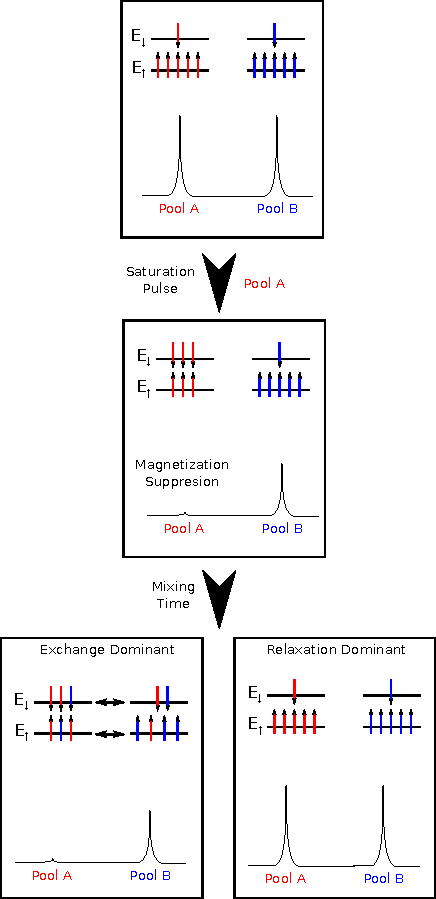
\includegraphics[width=0.4\textwidth]{cest/cest-images/cest_saturation.pdf}
\caption{\textbf{Summary of the CEST effect.} Initially two pools are considered, each with exchangeable protons.
The peaks correspond to the signal intensity from an image.
If a saturation pulse is applied with a saturation frequency at the resonance frequency of Pool A, the magnetization vector is decreased and signal intensity is suppressed.
Because of chemical exchange, the Pool B magnetization vector also decreases slightly.
If the system is dominated by relaxation (i.e.
if relaxation occurs as fast or faster than proton exchange) then the CEST effect is not observed the system recovers to its equilibrium state.
If the relaxation time is long relative to the exchange rate, a CEST effect is observed.
\newline \emph{\small{Image credit: adapted from Woods et al.~\cite{Woods:2006cq}}}}
\label{saturation}
\end{center}
\end{figure}
	
The CEST effect is only observed under specific conditions of exchange and relaxation.
At equilibrium, the spin population is distributed according to the Boltzmann distribution and the saturation pulse acts as a perturbation.
The longitudinal relaxation time (T$_1$) slowly counteracts this perturbation and if T$_1$ is short relative to the exchange rate (k$_{ex}$ describing proton transfer from Pool A to Pool B, the CEST effect is not observed~\cite{Woods:2006cq} and the system is dominated by relaxation (Fig.~\ref{saturation}).
A further criteria is that the exchange process must be slow relative to the NMR time scale,
	
	\begin{equation}
		\Delta \omega \geq k_{eq}
	\end{equation}

where $\Delta \omega$ is the difference between the Larmor frequencies of the two pools.
By saturating the bulk/free water pool, the magnetization from this pool is decreased and by saturation transfer, magnetization from the other pool also decreases.
From an imagine perspective, the net result is an overall darkening coupled with an increase in contrast as the difference between the two pools is increased.
Typically, negative contrast is not preferred in MR imaging because the human eye can more easily discriminate between a slight increase in image intensity than a similar decrease.
However, generation of this contrast can easily be controlled by turning off the saturation pulse prior to imaging.
Thus, data can be acquired with and without saturation, and post-processing techniques can be used to generate a `difference-image' consisting of positive contrast.

\subsection{APT-CEST}     

While there are several types of CEST contrasts available, in this
work we will focus our attention just on one subset, amide proton transfer or APT.
APT refers specifically to the chemical exchange between bulk-water protons and amide groups (-NH) of endogenous mobile peptides and proteins as it is most relevant for tumours~\cite{Togao:2013gn}.
The concentration of these mobile peptides and proteins is in the millimolar range and that has thusfar limited their utility to be considered a viable target for clinical diagnosis or prognosis, at least using MRI.
However due to the saturation transfer effect, APT imaging can be used to elucidate the presence of these mobile peptides and proteins~\cite{Zhou:2003cc}.
The APT effect arises when the amide groups on the protein backbones exchange with water protons after a saturation pulse directed at around 3.5 ppm with respect to water~\cite{vanZijl:2003in}.
Interestingly, the side chains of these same proteins and peptides comprising mostly the amino acids glutamine and asparagine that
resonate at about 2 ppm~\cite{vanZijl:2003in}.
Another potential contribution to the APT effect are the nucleosides that make up DNA and RNA molecules (nucleotides - adenosine, guanine, cytosine, uracil, thymine -  just without a phosphate group) but in their normal forms, the base pairs are hydrogen bonded so the exchange rates of those protons is very low (k$_{ex}$ < 0.01 s$^{-1}$) and these protons exchange very slowly with water.
When these DNA and RNA base pairs are caused to break down, denature, or separate, the labile protons are exposed and the concentration of exchageable protons increases resulting in a higher APT signal.
One can hypothesize that a treatment resulting in direct DNA damage and protein denaturation to expose additional hydrogens that could exchange with water would result in an APT signal increase in tumours.

Recently, CEST has been proposed to assess several the efficacy of several therapies and in this study we extend this work by first assessing the baseline variability of the APT effect, and then evaluate the efficacy of two treatments that may result in DNA damage (10Gy dose of whole-body radiation), as well as rapid loss of perfusion ultimately resulting in large-scale tumour necrosis (chemotherapy combretastatin)~\cite{Maxwell:2002da}.
Combretastatin is a a vascular targeting drug Combretastatin A-4 phosphate (CA4P) that has been shown to have both a strong acute effect at low dose, and a long term effect at high dose~\cite{Maxwell:2002da}.
To study the effect of these treatments on the APT CEST signal, an experiment was conducted to first assess the baseline repeatability (test-retest on subsequent days) of the APT CEST signal, followed by a treatment prior to the last imaging session.

\section{Development}

\subsection{MR Sequences}

\subsection{Phantom Work}

\subsection{Quantification \& Fitting}

\section{Methods}

\subsection{Animals}: NOD/SCID mice were implanted with a murine squamous cell carcinoma (SCCVII) on the left flank and tumours were allowed to grow until they reached 500mm$^3$.


\subsubsection{Experiment 1: CEST Controls + CA4P (CestS1)}

Animals were imaged daily for three days.
Then, 7 of those mice were injected i.p.
with 120$\mu$L of CA4P at a dose~\cite{Maxwell:2002da} of 80 mg/kg and imaged 24 hrs later.


\subsubsection{Experiment 2: CEST + 10Gy (CestS)}

5 mice received a 10Gy dose of radiation and were imaged 96 hours later (CestS2).


\subsubsection{Experiment 3: CEST + 40Gy (CestS3)}

5 mice received 40Gy dose of radiation and imaged 

Wednesday November 16, 2016 5 mice were irradiated with 40Gy but left at BCCRC for monitoring.
Mice were imaged and euthanized on Nov.
22nd, 2016.

\subsection{Imaging}

Imaging was performed using a 7T small animal scanner.
CEST scans were acquired using an EPI-based imaging scheme and continuous-wave saturation with B$_1$=1.0$\mu$T for 10s at each saturation frequency offset.
Spatial resolution of the CEST scan was 0.5 mm in-plane with a 1.5 mm slice thickness.
80 offset frequencies were acquired ranging from -20 to +20 ppm with a higher spectral resolution near peaks of interest.
Total scan time for the CEST sequence was 27 minutes.

\subsection{Histology}

\textbf{Histology:} Following the last imaging session, animals were injected with 50$\mu$L of the perfusion dye carbocyanine 5 minutes prior to sacrifice and the tumours were immediately excised and frozen.
Sequential sections 10$\mu$m thick were obtained every 0.5 mm and analysed to identify the fraction of perfused vessels and necrosis.
Sections were stained with TUNEL/CASPASE to mark apoptosis and CD31 to mark blood vessels.


\section{Results}

Figures~\ref{mainCest} \&~\ref{cestFractions} summarize the main results of the study, and the conclusions are summarized here:

\begin{enumerate}
\item While some changes in a subset of tumours can be observed in Figure~\ref{mainCest}, the tumour pixel distributions in the control groups are not statistically significantly different from the CA4P treatment group (red)

\item Histological evidence also did not point to a strong effect of treatment compared to the control groups~\ref{cestFractions}

\item Consequently, comparisons of the amine and amide peak sizes to histological fraction did not yield any conclusive correlations.

\end{enumerate}

\begin{figure}[htbp]
\begin{center}
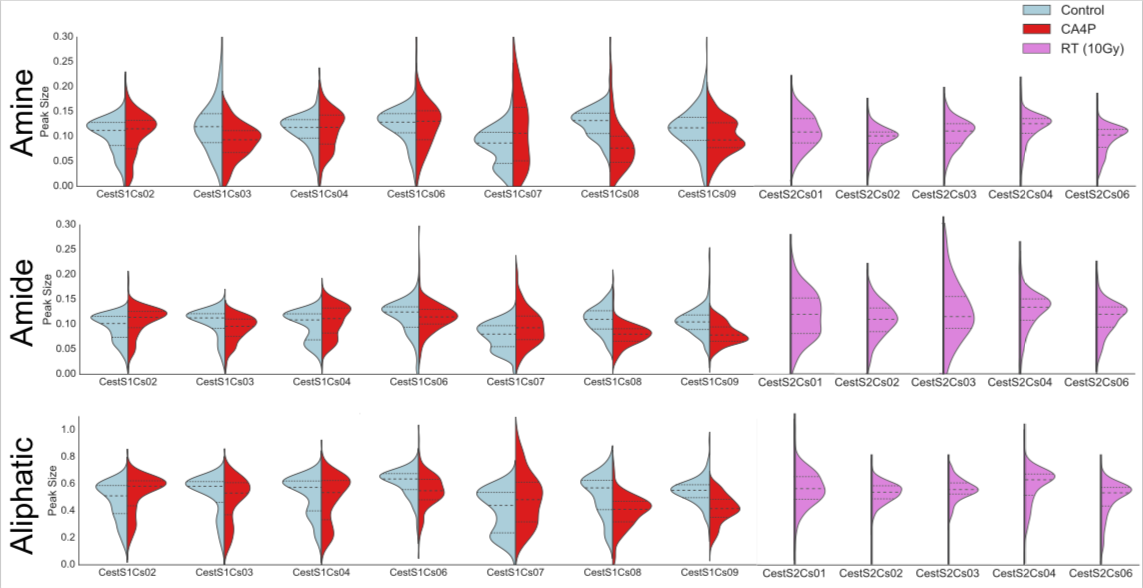
\includegraphics[width=\textwidth]{cest/cest-images/cest_Violinplots.png}
\caption{Peak-size (width x amplitude of peak) voxel distributions of every animal are shown as violin-plots for each of the three peaks of interest (amine at $\approx$2.2 ppm, amide at $\approx$3.5 ppm, and aliphatic at -3.5 ppm).
Colours represent the distribution at each treatment group: control (light blue), 24h post CA4P treatment (red), and 96h post 10Gy RT (violet).
Dashed lines within each half-violin corresponds to the median, and the dotted lines indicate the first and third quartiles.}
\label{mainCest}
\end{center}
\end{figure}

\begin{figure}[htbp]
\begin{center}
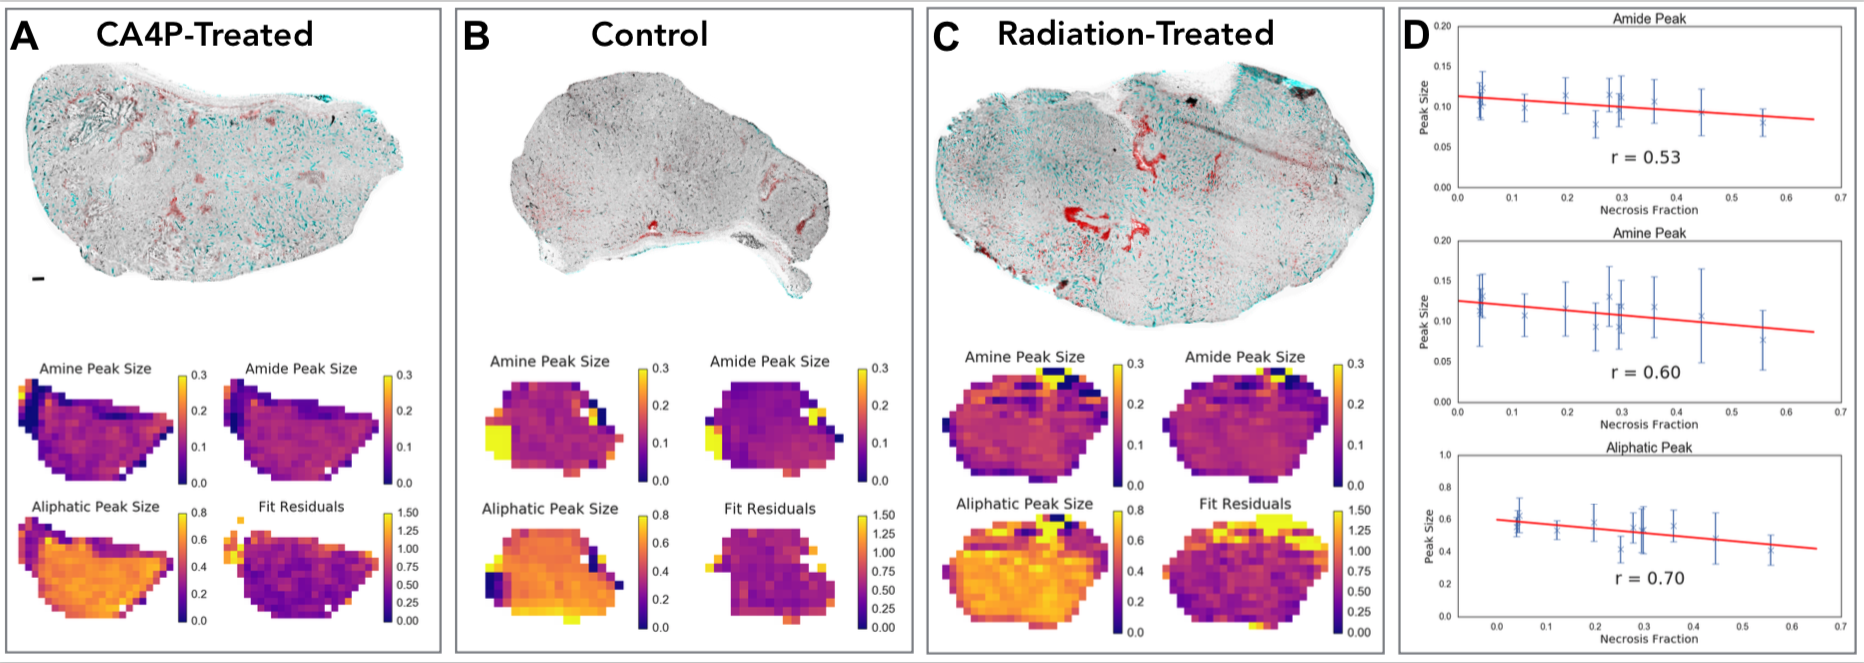
\includegraphics[width=\textwidth]{cest/cest-images/cest_RTstudy}
\caption{Representative histology sections are shown for each of the groups (A-C), as well as CEST parameter maps of a similar slice in the tumour.
CEST peak-size maps are shown for the amine, amide, aliphatic peaks as well as the fit residuals for each of the three groups.
The `fit-residual' maps were used to exclude voxels where fit quality was poor.
Necrosis fractions were calculated from the histology sections across all animals and treatment groups and plotted against the amine, amide, and aliphatic peak-sizes; r-values on the plots indicate the correlation coefficient.}
\label{cestFractions}
\end{center}
\end{figure}

%\section{Discussion}

%\section{Conclusions}


\endinput

Any text after an \endinput is ignored.
You could put scraps here or things in progress.

%%% The following is a directive for TeXShop to indicate the main file
%%!TEX root =../diss.tex

\chapter{Putting it all together}
\label{ch:meltingpot}

\section{Study 1: OEMRI \& HPG}


\section{Study 2: OEMRI and HPG and CEST} 

\endinput

%    3. Notes
%    4. Footnotes

%    5. Bibliography
\begin{singlespace}
\raggedright
\bibliographystyle{vancouver}
\bibliography{diss}
\end{singlespace}

\appendix
%    6. Appendices (including copies of all required UBC Research
%       Ethics Board's Certificates of Approval)
%\include{reb-coa}	% pdfpages is useful here
\chapter{Supporting Materials}

This would be any supporting material not central to the dissertation.
For example:
\begin{itemize}
\item additional details of methodology and/or data;
\item diagrams of specialized equipment developed.;
\item copies of questionnaires and survey instruments.
\end{itemize}


\backmatter
%    7. Index
% See the makeindex package: the following page provides a quick overview
% <http://www.image.ufl.edu/help/latex/latex_indexes.shtml>


\end{document}
